\documentclass[10pt,b5paper,]{book}
\usepackage{lmodern}
\usepackage{amssymb,amsmath}
\usepackage{ifxetex,ifluatex}
\usepackage{fixltx2e} % provides \textsubscript
\ifnum 0\ifxetex 1\fi\ifluatex 1\fi=0 % if pdftex
  \usepackage[T1]{fontenc}
  \usepackage[utf8]{inputenc}
\else % if luatex or xelatex
  \ifxetex
    \usepackage{mathspec}
  \else
    \usepackage{fontspec}
  \fi
  \defaultfontfeatures{Ligatures=TeX,Scale=MatchLowercase}
\fi
% use upquote if available, for straight quotes in verbatim environments
\IfFileExists{upquote.sty}{\usepackage{upquote}}{}
% use microtype if available
\IfFileExists{microtype.sty}{%
\usepackage{microtype}
\UseMicrotypeSet[protrusion]{basicmath} % disable protrusion for tt fonts
}{}
\usepackage[margin=1in]{geometry}
\usepackage{hyperref}
\hypersetup{unicode=true,
            pdftitle={Soil Organic Carbon Mapping cookbook},
            pdfborder={0 0 0},
            breaklinks=true}
\urlstyle{same}  % don't use monospace font for urls
\usepackage{natbib}
\bibliographystyle{apalike}
\usepackage{color}
\usepackage{fancyvrb}
\newcommand{\VerbBar}{|}
\newcommand{\VERB}{\Verb[commandchars=\\\{\}]}
\DefineVerbatimEnvironment{Highlighting}{Verbatim}{commandchars=\\\{\}}
% Add ',fontsize=\small' for more characters per line
\usepackage{framed}
\definecolor{shadecolor}{RGB}{248,248,248}
\newenvironment{Shaded}{\begin{snugshade}}{\end{snugshade}}
\newcommand{\AlertTok}[1]{\textcolor[rgb]{0.94,0.16,0.16}{#1}}
\newcommand{\AnnotationTok}[1]{\textcolor[rgb]{0.56,0.35,0.01}{\textbf{\textit{#1}}}}
\newcommand{\AttributeTok}[1]{\textcolor[rgb]{0.77,0.63,0.00}{#1}}
\newcommand{\BaseNTok}[1]{\textcolor[rgb]{0.00,0.00,0.81}{#1}}
\newcommand{\BuiltInTok}[1]{#1}
\newcommand{\CharTok}[1]{\textcolor[rgb]{0.31,0.60,0.02}{#1}}
\newcommand{\CommentTok}[1]{\textcolor[rgb]{0.56,0.35,0.01}{\textit{#1}}}
\newcommand{\CommentVarTok}[1]{\textcolor[rgb]{0.56,0.35,0.01}{\textbf{\textit{#1}}}}
\newcommand{\ConstantTok}[1]{\textcolor[rgb]{0.00,0.00,0.00}{#1}}
\newcommand{\ControlFlowTok}[1]{\textcolor[rgb]{0.13,0.29,0.53}{\textbf{#1}}}
\newcommand{\DataTypeTok}[1]{\textcolor[rgb]{0.13,0.29,0.53}{#1}}
\newcommand{\DecValTok}[1]{\textcolor[rgb]{0.00,0.00,0.81}{#1}}
\newcommand{\DocumentationTok}[1]{\textcolor[rgb]{0.56,0.35,0.01}{\textbf{\textit{#1}}}}
\newcommand{\ErrorTok}[1]{\textcolor[rgb]{0.64,0.00,0.00}{\textbf{#1}}}
\newcommand{\ExtensionTok}[1]{#1}
\newcommand{\FloatTok}[1]{\textcolor[rgb]{0.00,0.00,0.81}{#1}}
\newcommand{\FunctionTok}[1]{\textcolor[rgb]{0.00,0.00,0.00}{#1}}
\newcommand{\ImportTok}[1]{#1}
\newcommand{\InformationTok}[1]{\textcolor[rgb]{0.56,0.35,0.01}{\textbf{\textit{#1}}}}
\newcommand{\KeywordTok}[1]{\textcolor[rgb]{0.13,0.29,0.53}{\textbf{#1}}}
\newcommand{\NormalTok}[1]{#1}
\newcommand{\OperatorTok}[1]{\textcolor[rgb]{0.81,0.36,0.00}{\textbf{#1}}}
\newcommand{\OtherTok}[1]{\textcolor[rgb]{0.56,0.35,0.01}{#1}}
\newcommand{\PreprocessorTok}[1]{\textcolor[rgb]{0.56,0.35,0.01}{\textit{#1}}}
\newcommand{\RegionMarkerTok}[1]{#1}
\newcommand{\SpecialCharTok}[1]{\textcolor[rgb]{0.00,0.00,0.00}{#1}}
\newcommand{\SpecialStringTok}[1]{\textcolor[rgb]{0.31,0.60,0.02}{#1}}
\newcommand{\StringTok}[1]{\textcolor[rgb]{0.31,0.60,0.02}{#1}}
\newcommand{\VariableTok}[1]{\textcolor[rgb]{0.00,0.00,0.00}{#1}}
\newcommand{\VerbatimStringTok}[1]{\textcolor[rgb]{0.31,0.60,0.02}{#1}}
\newcommand{\WarningTok}[1]{\textcolor[rgb]{0.56,0.35,0.01}{\textbf{\textit{#1}}}}
\usepackage{longtable,booktabs}
\usepackage{graphicx,grffile}
\makeatletter
\def\maxwidth{\ifdim\Gin@nat@width>\linewidth\linewidth\else\Gin@nat@width\fi}
\def\maxheight{\ifdim\Gin@nat@height>\textheight\textheight\else\Gin@nat@height\fi}
\makeatother
% Scale images if necessary, so that they will not overflow the page
% margins by default, and it is still possible to overwrite the defaults
% using explicit options in \includegraphics[width, height, ...]{}
\setkeys{Gin}{width=\maxwidth,height=\maxheight,keepaspectratio}
\IfFileExists{parskip.sty}{%
\usepackage{parskip}
}{% else
\setlength{\parindent}{0pt}
\setlength{\parskip}{6pt plus 2pt minus 1pt}
}
\setlength{\emergencystretch}{3em}  % prevent overfull lines
\providecommand{\tightlist}{%
  \setlength{\itemsep}{0pt}\setlength{\parskip}{0pt}}
\setcounter{secnumdepth}{5}
% Redefines (sub)paragraphs to behave more like sections
\ifx\paragraph\undefined\else
\let\oldparagraph\paragraph
\renewcommand{\paragraph}[1]{\oldparagraph{#1}\mbox{}}
\fi
\ifx\subparagraph\undefined\else
\let\oldsubparagraph\subparagraph
\renewcommand{\subparagraph}[1]{\oldsubparagraph{#1}\mbox{}}
\fi

%%% Use protect on footnotes to avoid problems with footnotes in titles
\let\rmarkdownfootnote\footnote%
\def\footnote{\protect\rmarkdownfootnote}

%%% Change title format to be more compact
\usepackage{titling}

% Create subtitle command for use in maketitle
\newcommand{\subtitle}[1]{
  \posttitle{
    \begin{center}\large#1\end{center}
    }
}

\setlength{\droptitle}{-2em}
  \title{Soil Organic Carbon Mapping cookbook}
  \pretitle{\vspace{\droptitle}\centering\huge}
  \posttitle{\par}
  \author{}
  \preauthor{}\postauthor{}
  \predate{\centering\large\emph}
  \postdate{\par}
  \date{2018-02-22}

\usepackage{booktabs}
\usepackage{amsthm}
\makeatletter
\let\stdl@chapter\l@chapter
\renewcommand*{\l@chapter}[2]{%
  \stdl@chapter{\textcolor{astral}{#1}}{\textcolor{astral}{#2}}}

\def\thm@space@setup{%
  \thm@preskip=8pt plus 2pt minus 4pt
  \thm@postskip=\thm@preskip
}
\makeatother
\usepackage[table]{xcolor}
\usepackage{sectsty}

\definecolor{astral}{RGB}{153, 61, 15}
\allsectionsfont{\sffamily\color{astral}}

\hypersetup{
    colorlinks=true,
    linkcolor=astral,
    filecolor=astral,
    urlcolor=astral,
    citecolor=astral
}

\usepackage{fancyhdr}
\usepackage{pdfpages}

\renewcommand{\headrulewidth}{0.5pt}
\renewcommand{\headrule}{\hbox to\headwidth{\color{astral}\leaders\hrule height \headrulewidth\hfill}}

\pagestyle{fancy}
\fancyhf{}
\fancyhead[EL]{\nouppercase\leftmark}
\fancyhead[OR]{\nouppercase\rightmark}
\fancyhead[ER,OL]{\thepage}

\usepackage{multicol}

\usepackage{longtable}
\usepackage{array}
\usepackage{multirow}
\usepackage{wrapfig}
\usepackage{float}
\usepackage{colortbl}
\usepackage{pdflscape}
\usepackage{tabu}
\usepackage{threeparttable}
\usepackage[normalem]{ulem}


\makeatletter
\makeatother

\usepackage[sectionbib]{chapterbib}


\AtBeginDocument{\let\maketitle\relax}

\usepackage{amsthm}
\newtheorem{theorem}{Theorem}[chapter]
\newtheorem{lemma}{Lemma}[chapter]
\theoremstyle{definition}
\newtheorem{definition}{Definition}[chapter]
\newtheorem{corollary}{Corollary}[chapter]
\newtheorem{proposition}{Proposition}[chapter]
\theoremstyle{definition}
\newtheorem{example}{Example}[chapter]
\theoremstyle{definition}
\newtheorem{exercise}{Exercise}[chapter]
\theoremstyle{remark}
\newtheorem*{remark}{Remark}
\newtheorem*{solution}{Solution}
\begin{document}
\maketitle

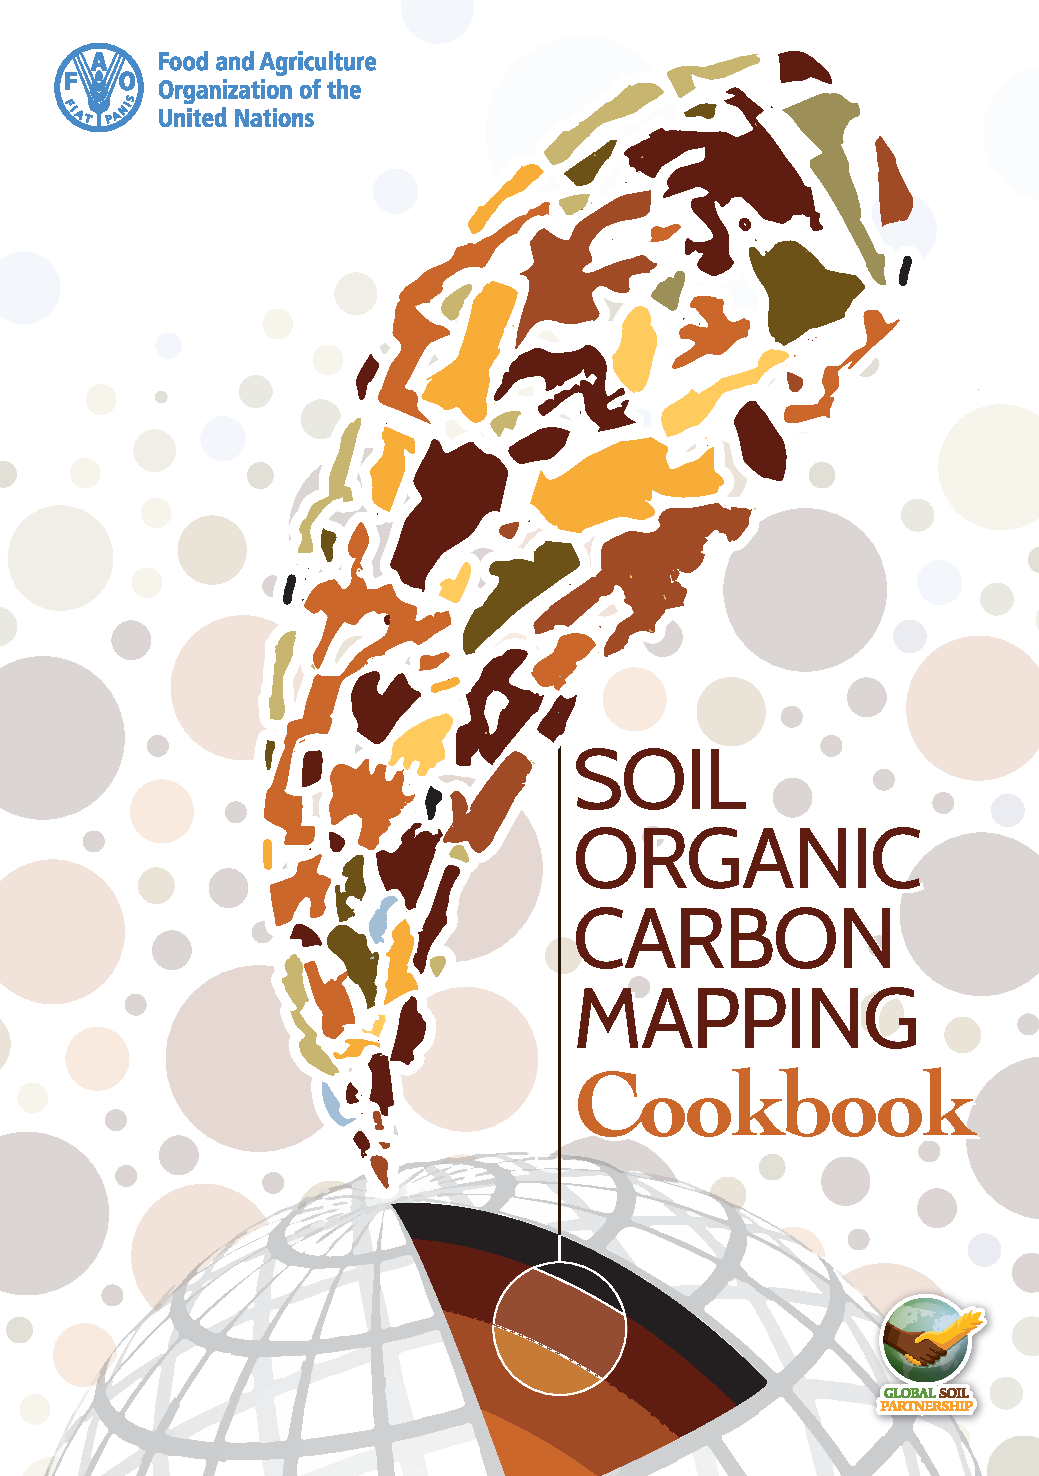
\includepdf{cover.pdf}

\frontmatter
\addtocontents{toc}{\protect\hypersetup{hidelinks}}
\addtocontents{lot}{\protect\hypersetup{hidelinks}}
\addtocontents{lof}{\protect\hypersetup{hidelinks}}

\hypertarget{copyright-and-disclaimer}{%
\chapter*{Copyright and disclaimer}\label{copyright-and-disclaimer}}
\addcontentsline{toc}{chapter}{Copyright and disclaimer}

\textbf{Recommended citation:}

\begin{quote}
FAO. 2018. Soil Organic Carbon Mapping Cookbook. Y Yigini, GF Olmedo, K
Viatkin, R Baritz, and RR Vargas, (Eds). 2nd edition, 2018.
\end{quote}

The designations employed and the presentation of material in this
information product do not imply the expression of any opinion
whatsoever on the part of the Food and Agriculture Organization of the
United Nations (FAO) concerning the legal or development status of any
country, territory, city or area or of its authorities, or concerning
the delimitation of its frontiers or boundaries. The mention of specific
companies or products of manufacturers, whether or not these have been
patented, does not imply that these have been endorsed or recommended by
FAO in preference to others of a similar nature that are not mentioned.

The views expressed in this information product are those of the
author(s) and do not necessarily reflect the views or policies of FAO.

ISBN {[}insert number{]}

\copyright FAO, 2018

FAO encourages the use, reproduction and dissemination of material in
this information product. Except where otherwise indicated, material may
be copied, downloaded and printed for private study, research and
teaching purposes, or for use in non-commercial products or services,
provided that appropriate acknowledgement of FAO as the source and
copyright holder is given and that FAO's endorsement of users' views,
products or services is not implied in any way.

All requests for translation and adaptation rights, and for resale and
other commercial use rights should be made via
www.fao.org/contact-us/licence-request or addressed to
\href{mailto:copyright@fao.org}{\nolinkurl{copyright@fao.org}}.

FAO information products are available on the
\href{www.fao.org/publications}{FAO website} and can be purchased
through
\href{mailto:publications-sales@fao.org}{\nolinkurl{publications-sales@fao.org}}.

\hypertarget{foreword-to-the-first-edition}{%
\chapter*{Foreword to the First
Edition}\label{foreword-to-the-first-edition}}
\addcontentsline{toc}{chapter}{Foreword to the First Edition}

This cookbook provides step-by-step guidance for developing 1 km grids
for soil carbon stocks. It includes the preparation of local soil data,
the compilation and pre-processing of ancillary spatial data sets,
upscaling methodologies, and uncertainty assessments. Guidance is mainly
specific to soil carbon data, but also contains many generic sections on
soil grid development, as it is relevant for other soil properties.

Therefore, this first edition is the beginning of a series of updates
and extensions, necessary to cover a larger variety of upscaling
approaches. Experiences gained throughout 2017 during the GSOC map
programme, through applications at country scale and various trainings
scheduled for 2017, shall be considered in the next editions. Also, the
section on uncertainties will be adjusted to more practical
implementation steps.

\hypertarget{foreword-to-the-second-edition}{%
\chapter*{Foreword to the Second
Edition}\label{foreword-to-the-second-edition}}
\addcontentsline{toc}{chapter}{Foreword to the Second Edition}

This edition has been updated with knowledge and practical experiences
gained during the implementation process of GSOCmap V1.0 throughout
2017. The cookbook includes step-by-step guidance for developing 1 km
grids for SOC stocks, as well as for the preparation of local soil data,
the compilation and preprocessing of ancillary spatial data sets,
upscaling methodologies, and uncertainty assessment methods. Guidance is
mainly specific to SOC data, but as this cookbook contains generic
sections on soil grid development it can be applicable to map various
soil properties.

\clearpage

\hypertarget{editorial-board}{%
\section*{Editorial Board}\label{editorial-board}}
\addcontentsline{toc}{section}{Editorial Board}

\begin{itemize}
\tightlist
\item
  Yusuf Yigini, Guillermo Federico Olmedo, Kostiantyn Viatkin, Rainer
  Baritz, Ronald R. Vargas Global Soil Partnership, Food and Agriculture
  Organization of the United Nations
\end{itemize}

\hypertarget{contributing-authors}{%
\section*{Contributing Authors}\label{contributing-authors}}
\addcontentsline{toc}{section}{Contributing Authors}

\begin{longtable}[]{@{}ll@{}}
\toprule
\endhead
\begin{minipage}[t]{0.13\columnwidth}\raggedright
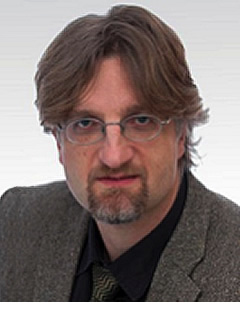
\includegraphics{contrAuthors/Baritz.jpg}\strut
\end{minipage} & \begin{minipage}[t]{0.81\columnwidth}\raggedright
Rainer Bartiz - Food and Agriculture Organization of the United
Nations\strut
\end{minipage}\tabularnewline
\begin{minipage}[t]{0.13\columnwidth}\raggedright
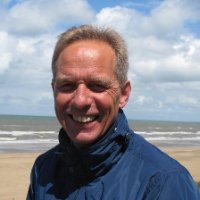
\includegraphics{contrAuthors/Brus.jpg}\strut
\end{minipage} & \begin{minipage}[t]{0.81\columnwidth}\raggedright
Dick Brus - Department of Plant Sciences, Wageningen University, the
Netherlands\strut
\end{minipage}\tabularnewline
\begin{minipage}[t]{0.13\columnwidth}\raggedright
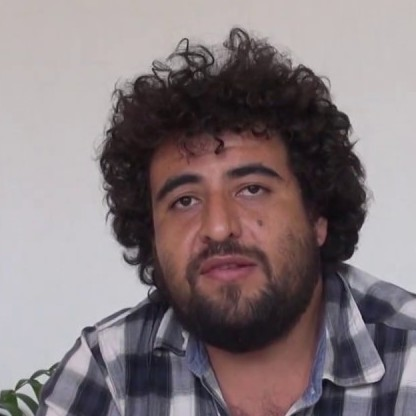
\includegraphics{contrAuthors/Guevara.jpg}\strut
\end{minipage} & \begin{minipage}[t]{0.81\columnwidth}\raggedright
Mario Guevara - University of Delaware, USA\strut
\end{minipage}\tabularnewline
\begin{minipage}[t]{0.13\columnwidth}\raggedright
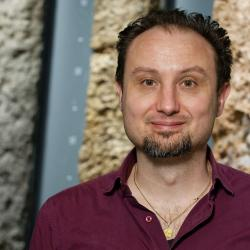
\includegraphics{contrAuthors/Hengl.jpg}\strut
\end{minipage} & \begin{minipage}[t]{0.81\columnwidth}\raggedright
Tomislav Hengl - ISRIC - World Soil Information, Wageningen, the
Netherlands\strut
\end{minipage}\tabularnewline
\begin{minipage}[t]{0.13\columnwidth}\raggedright
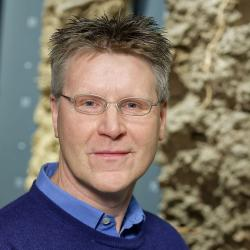
\includegraphics{contrAuthors/Heuvelink.jpg}\strut
\end{minipage} & \begin{minipage}[t]{0.81\columnwidth}\raggedright
Gerard Heuvelink - World Soil Information, Wageningen, the
Netherlands\strut
\end{minipage}\tabularnewline
\begin{minipage}[t]{0.13\columnwidth}\raggedright
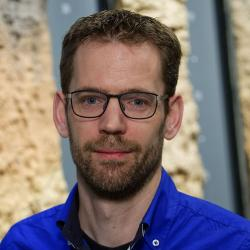
\includegraphics{contrAuthors/Kempen.jpg}\strut
\end{minipage} & \begin{minipage}[t]{0.81\columnwidth}\raggedright
Bas Kempen - ISRIC, World Soil Information, Wageningen, the
Netherlands\strut
\end{minipage}\tabularnewline
\begin{minipage}[t]{0.13\columnwidth}\raggedright
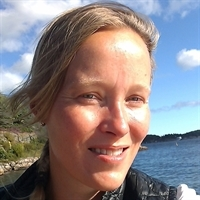
\includegraphics{contrAuthors/Mulder.jpeg}\strut
\end{minipage} & \begin{minipage}[t]{0.81\columnwidth}\raggedright
Titia VL Mulder - Wageningen University, Department of Environmental
Sciences, the Netherlands\strut
\end{minipage}\tabularnewline
\begin{minipage}[t]{0.13\columnwidth}\raggedright
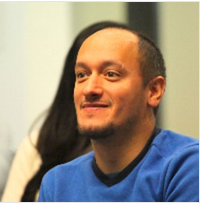
\includegraphics{contrAuthors/Olmedo.png}\strut
\end{minipage} & \begin{minipage}[t]{0.81\columnwidth}\raggedright
Guillermo Federico Olmedo - Instituto Nacional de Tecnología
Agropecuaria, Mendoza, Argentina\strut
\end{minipage}\tabularnewline
\begin{minipage}[t]{0.13\columnwidth}\raggedright
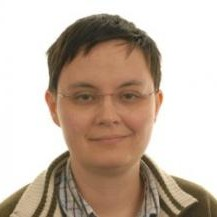
\includegraphics{contrAuthors/Poggio.jpg}\strut
\end{minipage} & \begin{minipage}[t]{0.81\columnwidth}\raggedright
Laura Poggio - The James Hutton Institute, Craigiebuckler Aberdeen,
Scotland UK\strut
\end{minipage}\tabularnewline
\begin{minipage}[t]{0.13\columnwidth}\raggedright
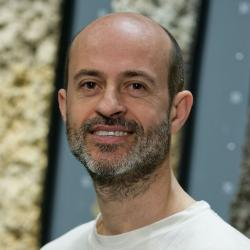
\includegraphics{contrAuthors/Ribeiro.jpg}\strut
\end{minipage} & \begin{minipage}[t]{0.81\columnwidth}\raggedright
Eloi Ribeiro - ISRIC , World Soil Information, Wageningen, the
Netherlands\strut
\end{minipage}\tabularnewline
\begin{minipage}[t]{0.13\columnwidth}\raggedright
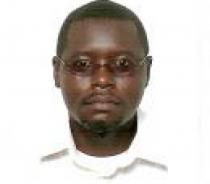
\includegraphics{contrAuthors/Omuto.jpg}\strut
\end{minipage} & \begin{minipage}[t]{0.81\columnwidth}\raggedright
Christian Thine Omuto - Department of Environmental and Biosystems
Engineering, University of Nairobi, Kenya\strut
\end{minipage}\tabularnewline
\begin{minipage}[t]{0.13\columnwidth}\raggedright
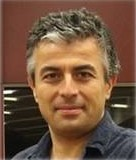
\includegraphics{contrAuthors/Yigini.jpg}\strut
\end{minipage} & \begin{minipage}[t]{0.81\columnwidth}\raggedright
Yusuf Yigini - Food and Agriculture Organization of the United
Nations\strut
\end{minipage}\tabularnewline
\begin{minipage}[t]{0.13\columnwidth}\raggedright
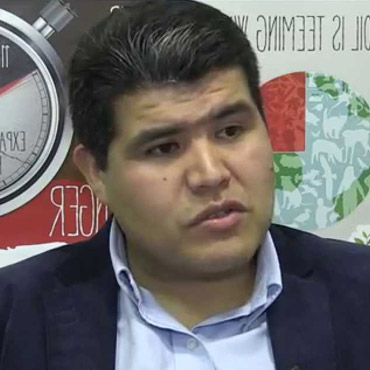
\includegraphics{contrAuthors/Vargas.jpg}\strut
\end{minipage} & \begin{minipage}[t]{0.81\columnwidth}\raggedright
Ronald R Vargas - Food and Agriculture Organization of the United
Nations\strut
\end{minipage}\tabularnewline
\bottomrule
\end{longtable}

\mainmatter
\tableofcontents
\listoffigures
\listoftables

\hypertarget{presentation}{%
\chapter{Presentation}\label{presentation}}

Soils provide ecosystem services critical to life on Earth. The Food and
Agricultural Organization of the United Nations (FAO) recognizes the
need to preserve soil resources from degradation and restore them. In
2012, the Global Soil Partnership (GSP) was established to improve soil
governance and promote sustainable soil management.

The GSP aims to promote sustainable soil management at all levels
globally through normative tools relying on evidence-based science.
Understanding the status of a given soil in different land uses,
including its properties and functions, and relating this information to
the various ecosystem services provided by soils, becomes mandatory for
sustainable soil management decisions. As the availability and use of
soil data and information is fundamental to underpin these decisions,
members of the GSP decided to establish a Global Soil Information System
(GLOSIS) based on the development of national soil information systems.

In the process of establishing GLOSIS, a number of tools and networks
are being created, including the International Network of Soil
Information Institutions (INSII), a
\href{http://www.fao.org/3/a-bs975e.pdf}{\emph{GSP Soil Data Policy}}
and more. Taking advantage of this process and responding to a request
for support in addressing the Sustainable Development Goal Indicators,
especially indicator 15.3 which includes the restoration of degraded
soils, the GSP Plenary Assembly in 2016 instructed the Intergovernmental
Technical Panel on Soils (ITPS) and the GSP Secretariat to develop the
first-ever Global Soil Organic Carbon Map (GSOCMap) following the same
bottom-up approach as GLOSIS. To this end, members under the INSII
umbrella developed guidelines and technical specifications for the
preparation of the \href{http://www.fao.org/3/a-bp164e.pdf}{GSOCMap} and
countries were invited to prepare their national soil organic carbon
maps according to these specifications.

Given the scientific advances in tools for mapping soil organic carbon
(SOC), many countries requested the GSP Secretariat to support them in
the process of preparing national maps, hence an intensive capacity
development programme on SOC mapping has been implemented to support
countries in this process. Various regional and national training
sessions were organized using an on-the-job-training modality to ensure
national experts were trained to utilize their own datasets to produce
reliable SOC maps. The GSP Secretariat invited a group of experts to
prepare a \emph{Soil Organic Carbon Mapping Cookbook} as a
comprehensible reference knowledge source to support the capacity
development process.

The second edition of the cookbook provides generic methodologies and
technical steps to produce SOC maps. This edition has been updated with
knowledge and practical experiences gained during the implementation
process of GSOCmap V1.0 throughout 2017. The cookbook includes
step-by-step guidance for developing 1 km grids for SOC stocks, as well
as for the preparation of local soil data, the compilation and
preprocessing of ancillary spatial data sets, upscaling methodologies,
and uncertainty assessment methods. Guidance is mainly specific to SOC
data, but as this cookbook contains generic sections on soil grid
development it can be applicable to map various soil properties.

The guidance is focusing on the upscaling of national SOC stocks in
order to produce the GSOCMap. Therefore, the cookbook supplements the
\href{http://www.fao.org/3/a-bp164e.pdf}{\emph{GSP Guidelines for
Sharing National Data/Information to Compile a Global Soil Organic
Carbon (GSOC) Map}}, providing technical guidelines to prepare and
evaluate spatial soil data sets to:

\begin{itemize}
\tightlist
\item
  Determine SOC stocks from local samples to a target depth of 30 cm;
\item
  Prepare spatial covariates for upscaling; and
\item
  Select and apply the best suitable upscaling methodology.
\end{itemize}

In terms of statistical upscaling methods, the use of conventional
upscaling methods using soil maps and soil profiles is still very
common, although this approach is mostly considered empirical by soil
mappers. Even though evaluations are based on polygon soil maps, the
resulting SOC maps can be rasterized to any target grid. However, a
spatially-explicit assessment of uncertainties is impossible. The use of
digital soil mapping to upscale local soil information is increasingly
applied and recommended.

This cookbook presents two approaches in detail, namely spatial
modelling using either regression or data mining analysis, combined with
geostatistics such as regression kriging. The second edition includes
updates in the section on uncertainty assessment.

It is our hope that this cookbook will fulfill its mandate of easily
enabling any user to produce a digital SOC or other soil property map
using soil legacy data and modern methods of digital soil mapping with
the overall aim for improved decision making on soil management.

\hypertarget{soil-property-maps}{%
\chapter{Soil Property Maps}\label{soil-property-maps}}

\emph{R Baritz}

\hypertarget{definitions-and-objectives}{%
\section{Definitions and Objectives}\label{definitions-and-objectives}}

Soil property maps represent spatial information about soil properties
to a certain depth or for soil horizons. Conventionally, soil property
maps are generated as polygon maps, with properties from typical soil
profiles representing soil mapping units. Digital Soil Mapping (DSM)
allows more accurate spatial mapping of soil properties, including the
spatial quantification of the prediction error. The quality of such
predictions improves with increasing number of local observations
(e.g.~soil profiles) available to build the prediction model. Whenever
possible, DSM is recommended.

The development of soil property maps via DSM is spatially flexible. For
different soil properties (e.g.~concentration and stocks of nutrients in
the soil, carbon, heavy metals, pH, cation exchange capacity, physical
soil properties such as particle sizes and bulk density, etc.), various
depth classes and spatial resolution can be modeled depending on project
and mapping objectives and available input data. For GSOCmap, a 1 km
grid is pursued. The same methodology and input data can also be used to
produce higher resolution soil grids.

The mapping of global soil organic carbon (GSOC) stocks will be the
first implementation of a series of other soil property grids to be
developed for GLOSIS, based on the typical GSP country-driven system.
GSOCmap will demonstrate the capacity of countries all around the globe
to compile and manage national soil information systems and to utilize
and evaluate these data following agreed international specifications.
The GSP Secretariat, FAO, and its regional offices, as well as the
Regional Soil Partnerships, are challenged together with the GSP
members, especially the members of INSII, to establish national capacity
and soil data infrastructures to enable soil property mapping.

\hypertarget{generic-mapping-of-soil-grids-upscaling-of-plot-level-measurements-and-estimates}{%
\section{Generic Mapping of Soil Grids: Upscaling of Plot-Level
Measurements and
Estimates}\label{generic-mapping-of-soil-grids-upscaling-of-plot-level-measurements-and-estimates}}

The following table presents an overview of different geographic
upscaling approaches, recommended to produce soil property maps, in
particular, GSOCmap.

\begin{longtable}[]{@{}lll@{}}
\toprule
\endhead
\begin{minipage}[t]{0.20\columnwidth}\raggedright
Conventional upscaling \citep{lettens2004soil}\strut
\end{minipage} & \begin{minipage}[t]{0.27\columnwidth}\raggedright
Class-matching\strut
\end{minipage} & \begin{minipage}[t]{0.44\columnwidth}\raggedright
Derive average SOC stocks per class: soil type for which a national map
exists, or combination with other spatial covariates (e.g.~land use
category, climate type, biome, etc.). This approach is used in the
absence of spatial coordinates of the source data.\strut
\end{minipage}\tabularnewline
\begin{minipage}[t]{0.20\columnwidth}\raggedright
\strut
\end{minipage} & \begin{minipage}[t]{0.27\columnwidth}\raggedright
Geomatching\strut
\end{minipage} & \begin{minipage}[t]{0.44\columnwidth}\raggedright
Point locations with spatial referencing are overlaid with GIS layers of
important covariates (e.g.~a soil map). Upscaling is based on averaged
SOC values per mapping unit.\strut
\end{minipage}\tabularnewline
\begin{minipage}[t]{0.20\columnwidth}\raggedright
Digital soil mapping \citep{dobos2006digital}\strut
\end{minipage} & \begin{minipage}[t]{0.27\columnwidth}\raggedright
Data mining and geostatistics\strut
\end{minipage} & \begin{minipage}[t]{0.44\columnwidth}\raggedright
Multiple regression, classification tree, random forests, regression
kriging, kriging with external drift.\strut
\end{minipage}\tabularnewline
\bottomrule
\end{longtable}

Digital soil mapping is based on the development of functions for
upscaling point data (with soil measurements) to a full spatial extent
using correlated environmental covariates, for which spatial data are
available.

\begin{quote}
DSM: Concept of environmental correlation that explores the quantitative
relationship between environmental variables and soil properties and
could be used to predict the latter with multivariate prediction
techniques.
\end{quote}

\hypertarget{preparation}{%
\chapter{Preparation of Local Soil Data}\label{preparation}}

\emph{GF Olmedo \& R Baritz}

\hypertarget{soil-profiles-and-soil-augers}{%
\section{Soil Profiles and Soil
Augers}\label{soil-profiles-and-soil-augers}}

Soil profiles are complex real-world entities. They are composed of soil
layers which form soil horizons; the soil layers have different
properties and these properties are evaluated with different methods. As
we know, soil and vertical soil properties are landscape elements and
part of matter dynamics (water, nutrients, gases, habitat, etc.). Local
soil samples or soil profiles add a third dimension into the spatial
assessment of soil properties in the landscape.

Most \emph{commonly}, soils are described as vertical profiles using
soil pits (sometimes also augerings, but this is less accurate). Soil
profiles are described using macro-morphological properties. These
properties can be assessed in the field without analysis by making a
field inventory or land evaluation. For additional quantitative
analysis, soils are then sampled by genetic horizons or by depth class.

The sampling of soils is the basis to obtain quantitative information.
Depending on the goal of a project, sampling can be quite diverse.
Sampling can follow the description of the soil or can be conducted
without, for example using a spade or auger to generate a composite
sample (for a certain depth independent of the morphological features
such as soil horizons). Sampling locations can be representative of a
certain location, project, field, or mapped object, such as a soil type.

\hypertarget{soil-database}{%
\section{Soil Database}\label{soil-database}}

In order to process and evaluate soil information from field
assessments, soil profile data and analytical information need to be
stored in a database. This can be a set of simple \emph{Excel}
spreadsheets, or a relational or object-oriented database management
system \citep{baritz2008environmental}. When working in \textbf{R},
\texttt{SoilProfileCollections} from the \textbf{R} \textbf{aqp} package
are a useful tool. Tables \ref{tab:site-level} and
\ref{tab:horizon-level} are examples of how soil information can be
stored. The advantage of such organization is the possibility to develop
relational databases which can be easily queried. Such a systematic
approach will support the organization of national soil information and
will reduce errors in future modeling exercises
\citep{baritz2008environmental}.

Table \ref{tab:site-level} stores site-level data, which describe the
location of the soil description and/or sampling site: spatial
coordinates, landscape attributes such as slope gradient and slope form,
soil class, land cover type, rock type, etc. In this table, every row
should hold a single soil profile. One column, usually the first one,
should be the soil profile's unique identifier. Using the latter, soil
information can be easily linked from one table to another.

\begin{table}

\caption{\label{tab:site-level}Example for site-level data table}
\centering
\begin{tabular}[t]{lrrrl}
\toprule
ProfID & X\_coord & Y\_coord & Year & Soil\_Type\\
\midrule
P1276 & 7591265 & 4632108 & 2012 & Complex of Chernozem …\\
P1277 & 7592027 & 4631664 & 2012 & Complex of Chernozem …\\
P1278 & 7592704 & 4631941 & 2012 & Complex of Chernozem …\\
P1279 & 7590817 & 4633115 & 2013 & Complex of Chernozem …\\
\bottomrule
\end{tabular}
\end{table}

Table \ref{tab:horizon-level} stores information from the soil
description, such as horizon name, horizon thickness, organic matter
content, carbonate content, soil color, laboratory soil analysis, etc.
The first column contains the soil profile's unique identifier. It is
important to include the upper and lower limits for each soil layer; in
case the sampling strategy deviates from soil layers/soil horizons, the
upper and lower depth of the sampling locations should be specified if
possible. This information is needed for modeling soil properties over
the soil profile.

\begin{table}

\caption{\label{tab:horizon-level}Example for profile-description table}
\centering
\begin{tabular}[t]{llrrrrrrrr}
\toprule
ProfID & HorID & top & bottom & SOC & BLD & CRF & Sand & Silt & Clay\\
\midrule
P1276 & P1276H01 & 0 & 50 & 2.78 & 1.05 & 11 & 52 & 39 & 9\\
P1276 & P1276H02 & 50 & 76 & 1.75 & 1.45 & 4 & 56 & 31 & 14\\
P1276 & P1276H03 & 76 & 100 & 1.19 & 1.22 & 2 & 43 & 35 & 22\\
P1277 & P1277H01 & 0 & 28 & 1.93 & 1.36 & 8 & 59 & 22 & 18\\
P1277 & P1277H02 & 28 & 48 & 1.60 & 1.43 & 9 & 69 & 15 & 16\\
\addlinespace
P1277 & P1277H03 & 48 & 63 & 1.26 & NA & 25 & 65 & 21 & 13\\
P1277 & P1277H04 & 63 & 120 & 0.86 & NA & 54 & 63 & 23 & 14\\
P1278 & P1278H01 & 0 & 40 & 2.32 & 1.27 & 0 & 50 & 39 & 12\\
P1278 & P1278H02 & 40 & 68 & 1.80 & 1.48 & 1 & 46 & 39 & 16\\
P1278 & P1278H03 & 68 & 120 & 0.89 & 1.18 & 0 & 47 & 39 & 14\\
\bottomrule
\end{tabular}
\end{table}

\hypertarget{technical-steps---loading-data-from-tables-in-r}{%
\subsection{Technical Steps - Loading Data from Tables in
R}\label{technical-steps---loading-data-from-tables-in-r}}

This chapter includes two examples for data preparation. The first
example is for using soil profiles data. This example is mixed with the
text but a copy the code is presented in section
\ref{cd:PreparationProfiles}. The second example is using topsoil or
auger data and is presented in section \ref{cd:PreparationAuger}.

\begin{Shaded}
\begin{Highlighting}[]
\NormalTok{dat <-}\StringTok{ }\KeywordTok{read.csv}\NormalTok{(}\DataTypeTok{file =} \StringTok{"data/horizons.csv"}\NormalTok{)}

\CommentTok{# Explore the data}
\KeywordTok{str}\NormalTok{(dat)}
\KeywordTok{summary}\NormalTok{(dat)}
\end{Highlighting}
\end{Shaded}

\begin{verbatim}
## 'data.frame':    10292 obs. of  10 variables:
##  $ ProfID: Factor w/ 4118 levels "P0000","P0001",..: 1 1 1 2 2 ..
##  $ HorID : Factor w/ 9914 levels "P0000H01","P0000H02",..: 1 2 ..
##  $ top   : int  4 23 46 2 11 0 22 63 0 3 ...
##  $ bottom: int  23 46 59 11 31 22 63 90 19 10 ...
##  $ SOC   : num  NA NA NA NA NA ...
##  $ BLD   : num  NA NA NA NA NA NA NA NA NA NA ...
##  $ CRF   : num  54 62 47 66 70 57 77 87 8 4 ...
##  $ SAND  : int  52 59 67 45 40 52 48 43 50 48 ...
##  $ SILT  : num  34 31 24 39 31 33 36 42 16 35 ...
##  $ CLAY  : num  14 11 8 16 28 15 16 16 34 17 ...
##      ProfID           HorID            top        
##  P2881  :   64   P2881H01:   64   Min.   :  0.00  
##  P1481  :   32   P0434H02:    8   1st Qu.:  0.00  
##  P2096  :   32   P1286H01:    8   Median : 20.00  
##  P3623  :   32   P2056H01:    8   Mean   : 27.48  
##  P2056  :   24   P2056H02:    8   3rd Qu.: 47.00  
##  P2142  :   24   P2056H03:    8   Max.   :285.00  
##  (Other):10084   (Other) :10188                   
##      bottom            SOC              BLD      
##  Min.   :  1.00   Min.   : 0.000   Min.   :0.00  
##  1st Qu.: 25.00   1st Qu.: 1.090   1st Qu.:1.40  
##  Median : 45.00   Median : 1.800   Median :1.54  
##  Mean   : 55.82   Mean   : 2.603   Mean   :1.55  
##  3rd Qu.: 80.00   3rd Qu.: 2.940   3rd Qu.:1.66  
##  Max.   :295.00   Max.   :83.820   Max.   :2.93  
##                   NA's   :831      NA's   :7845  
##       CRF             SAND             SILT      
##  Min.   :  0.0   Min.   :  0.00   Min.   : 0.00  
##  1st Qu.:  2.0   1st Qu.: 44.00   1st Qu.:16.00  
##  Median :  8.0   Median : 58.00   Median :24.00  
##  Mean   : 13.5   Mean   : 57.67   Mean   :25.64  
##  3rd Qu.: 21.0   3rd Qu.: 72.00   3rd Qu.:33.00  
##  Max.   :104.0   Max.   :100.00   Max.   :80.00  
##  NA's   :3360    NA's   :1049     NA's   :920    
##       CLAY      
##  Min.   : 0.00  
##  1st Qu.: 7.00  
##  Median :14.00  
##  Mean   :17.08  
##  3rd Qu.:24.00  
##  Max.   :83.00  
##  NA's   :927
\end{verbatim}

\begin{Shaded}
\begin{Highlighting}[]
\NormalTok{dat_sites <-}\StringTok{ }\KeywordTok{read.csv}\NormalTok{(}\DataTypeTok{file =} \StringTok{"data/site-level.csv"}\NormalTok{)}

\CommentTok{# Explore the data}
\KeywordTok{str}\NormalTok{(dat_sites)}
\end{Highlighting}
\end{Shaded}

\begin{verbatim}
## 'data.frame':    4118 obs. of  6 variables:
##  $ X.1       : int  1 2 3 4 5 6 7 8 9 10 ...
##  $ ProfID    : Factor w/ 4118 levels "P0000","P0001",..: 1 2 3 ..
##  $ soiltype  : Factor w/ 58 levels "Albic Luvisol",..: 3 3 3 57..
##  $ Land.Cover: int  25 24 25 26 26 27 27 27 22 23 ...
##  $ X         : num  20.8 20.8 20.8 20.8 20.8 ...
##  $ Y         : num  42 42 42 42 42 ...
\end{verbatim}

\hypertarget{completeness-of-measurements-and-estimates}{%
\section{Completeness of Measurements and
Estimates}\label{completeness-of-measurements-and-estimates}}

The \emph{GSP Guidelines for Sharing National Data/Information to
Compile a Global Soil Organic Carbon (GSOC) Map} specify which soil
parameters are needed to produce a GSOCmap. Of course, other soil
properties can be evaluated and modeled using this cookbook as well.

SOC stocks for soil horizons or targeted soil depths can be calculated
using the equations in section 8.4.3 of the \emph{GSP Guidelines for
Sharing National Data/Information to Compile a Global Soil Organic
Carbon (GSOC) Map}. Carbon concentration, bulk density and stone content
for a certain depth or genetic horizon are needed to calculate the
amount of carbon stored in that depth interval/soil horizon. In many
countries, legacy data from former surveys and projects, as well as from
various owners and data sources are compiled. Often, measured bulk
densities are either missing, only available for few soil profiles, or
are estimated. Stones in the soil profile are usually only estimated,
and if augers are used for sampling, stone content is not assessed at
all. Pedo-transfer functions can be used to fill data gaps (e.g.~bulk
density), and interpolation approaches can be used to infer from
measured depths to target depths.

\hypertarget{stones}{%
\subsection{Stones}\label{stones}}

The estimation of stoniness is difficult and time-consuming, and
therefore not carried out in many national soil inventories, or only
estimated visually in the profile. Unfortunately, if soil inventories
and sampling are done with simple pits or augers rather than standard
soil pits, stones are very often not assessed.

As a proxy, it is recommended to derive national default values from
well-described soil profile pits by soil type.

\begin{Shaded}
\begin{Highlighting}[]
\CommentTok{# summary of column CRF (Coarse Fragments) in the example data base}
\KeywordTok{summary}\NormalTok{(dat}\OperatorTok{$}\NormalTok{CRF)}
\end{Highlighting}
\end{Shaded}

\begin{verbatim}
##    Min. 1st Qu.  Median    Mean 3rd Qu.    Max.    NA's 
##     0.0     2.0     8.0    13.5    21.0   104.0    3360
\end{verbatim}

\begin{Shaded}
\begin{Highlighting}[]
\CommentTok{# Convert NA's to 0}
\NormalTok{dat}\OperatorTok{$}\NormalTok{CRF[}\KeywordTok{is.na}\NormalTok{(dat}\OperatorTok{$}\NormalTok{CRF)] <-}\StringTok{ }\DecValTok{0}

\KeywordTok{hist}\NormalTok{(dat}\OperatorTok{$}\NormalTok{CRF, }\DataTypeTok{col =} \StringTok{"light gray"}\NormalTok{)}
\end{Highlighting}
\end{Shaded}

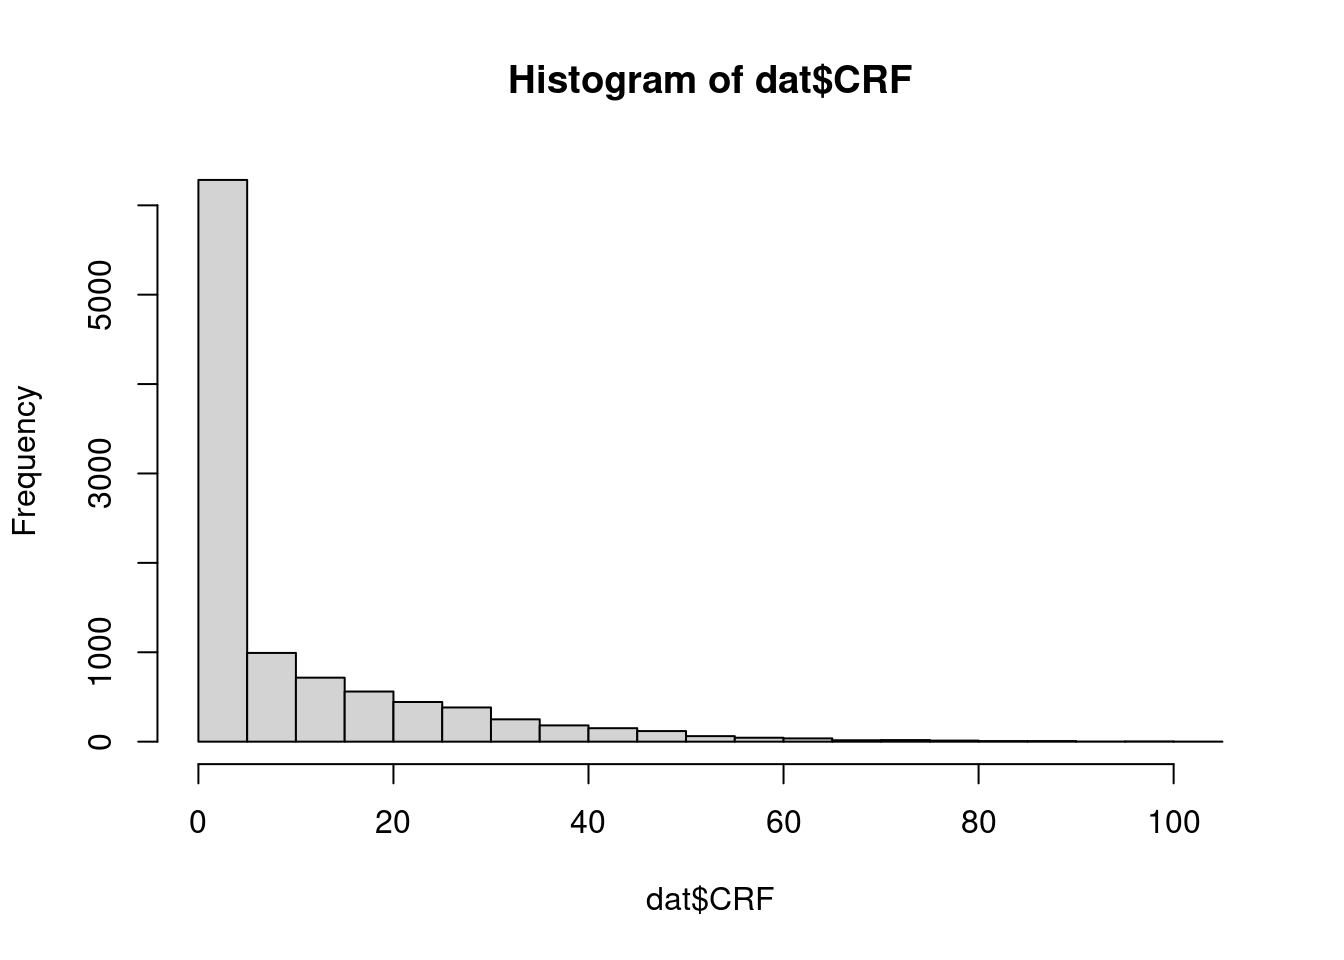
\includegraphics{SOCMapping_files/figure-latex/unnamed-chunk-3-1.pdf}

\hypertarget{bulk-density}{%
\subsection{Bulk density}\label{bulk-density}}

The amount of fine earth is one of the basic estimation parameters to
estimate SOC stocks in the mineral soil as well as in peat layers. It
depends on the volume of soil considered
(\(\text{depth} \times \text{reference area}\)) and the bulk density
(BD). BD expresses the soil weight per unit volume. When determining BD,
it is important to subtract stones, if any, from the cylinder samples;
if this is not done, BD is underestimated, and the resulting SOC stocks
are overestimated. Stones in the cylinders are added to the total stone
content in order to correct for the total amount of fine earth per
volume of soil in a given area.

Most of the soil profiles in national databases come from agricultural
land. Very often, BD estimates do not consider fine stones because top
soils (e.g.~plough layers) seem to be free of visible stones.

\textbf{Mineral soil}: Default values from
\href{https://www.nrcs.usda.gov/wps/portal/nrcs/detail/soils/survey/office/ssr10/tr/?cid=nrcs144p2_074844}{\emph{General
Guide for Estimating Moist Bulk Density}}. If analytical BD is missing,
BD can be estimated using pedo-transfer functions (see examples listed
below).

For organic soil material, \(BD_x\) can be estimated as follows,
considering existing litter layers L (or Oi horizon); organic or duff
layers, partially decomposed material above the mineral soil and beneath
the litter layer; F (fermentation) horizons; H (humus) horizons (Oe and
Oa); and peat (P), as described in the
\href{https://www.nrcs.usda.gov/Internet/FSE_DOCUMENTS/nrcs142p2_051232.pdf}{\emph{U.S.
Soil Taxonomy}}.

\textbf{Forest floor}: Default values from \citet{ottmar_litter_2007}.

\begin{itemize}
\item
  Pine: \(BD_{L} = 0.018 g \cdot cm^{-3}\);
  \(BD_{F,H} = 0.057 g \cdot cm^{-3}\)
\item
  Hardwood: \(BD_{L} = 0.012 g \cdot cm^{-3}\)
  \citep{barney_forest_1981}
\item
  Birch: \(BD_{F,H} = 0.17 g \cdot cm^{-3}\)
\item
  Spruce: \(BD_{L} = 0.051 g \cdot cm^{-3}\);
  \(BD_{H}= 0.13 g \cdot cm^{-3}\)
\end{itemize}

\textbf{Peat}: Default value: \(BD_{P} = 0.31 g \cdot cm^{-3}\). The
range of peat BD is generally from 0.02 to 0.3 \(t \cdot m^{-3}\)
depending on maturity and compaction, as well as the ash content
\citep{agus_measuring_2011}.@batjes1996total and
\citet{agus_measuring_2011} distinguish different peat decomposition
types (with different C content):

\begin{itemize}
\item
  Sapric: \(BD_{P,\text{sapric}} = 0.174 g \cdot cm^{-3}\) (\(48.90\%\)
  C)
\item
  Hemic: \(BD_{P,\text{hemic}} = 0.117 g \cdot cm^{-3}\) (\(52.27\%\) C)
\item
  Fibric: \(BD_{P,\text{fibric}} = 0.089 g \cdot cm^{-3}\) (\(53.56\%\)
  C)
\end{itemize}

Examples for pedo-transfer functions to estimate \(BD\), based on the
soil organic matter (\(OM\)) content in percent \((\%)\):

\begin{equation}
BD = 1.62-0.06 * OM
\end{equation}

\cite{saini_1966_organic}

\begin{equation}
BD = 1/(0.6268 + 0.0361 * OM)
\end{equation}

\cite{Drew1973}

\begin{equation}
BD = 1.482 - 0.6786 * (log OM)
\end{equation}

\cite{jeffrey1970note}

\begin{equation}
BD = 0.669 + 0.941 * e^{(-0,06 * OM)}
\end{equation}

\cite{Grigal1989}

\begin{equation}
BD = 100/(OM/0.244 + (100-OM))/MBD
\end{equation}

\cite{adams1973effect}

\begin{equation}
BD = 1/(0.564 + 0.0556*OM)
\end{equation}

\cite{honeysett1989use}

where \(MDB\) is the mineral particle density, assumed to be the
specific gravity of quartz, \(2.65 Mg \cdot m^{-3}\). And \(OM\) is the
organic matter content, estimated as \(OM = SOC(\%) × 1.724\)

Each method is derived from a specific set of regional soils that is
regionally adapted. Selection of the proper method for a given country
shall be based on existing reviews and comparisons.

\begin{Shaded}
\begin{Highlighting}[]
\CommentTok{# Creating a function in R to estimate BLD using the SOC}
\CommentTok{# SOC is the soil organic carbon content in \textbackslash{}%}
\NormalTok{estimateBD <-}\StringTok{ }\ControlFlowTok{function}\NormalTok{(SOC, }\DataTypeTok{method=}\StringTok{"Saini1996"}\NormalTok{)\{}
\NormalTok{  OM <-}\StringTok{ }\NormalTok{SOC }\OperatorTok{*}\StringTok{ }\FloatTok{1.724}
  \ControlFlowTok{if}\NormalTok{(method}\OperatorTok{==}\StringTok{"Saini1996"}\NormalTok{)\{BD <-}\StringTok{ }\FloatTok{1.62} \OperatorTok{-}\StringTok{ }\FloatTok{0.06} \OperatorTok{*}\StringTok{ }\NormalTok{OM\}}
  \ControlFlowTok{if}\NormalTok{(method}\OperatorTok{==}\StringTok{"Drew1973"}\NormalTok{)\{BD <-}\StringTok{ }\DecValTok{1} \OperatorTok{/}\StringTok{ }\NormalTok{(}\FloatTok{0.6268} \OperatorTok{+}\StringTok{ }\FloatTok{0.0361} \OperatorTok{*}\StringTok{ }\NormalTok{OM)\}}
  \ControlFlowTok{if}\NormalTok{(method}\OperatorTok{==}\StringTok{"Jeffrey1979"}\NormalTok{)\{BD <-}\StringTok{ }\FloatTok{1.482} \OperatorTok{-}\StringTok{ }\FloatTok{0.6786} \OperatorTok{*}\StringTok{ }\NormalTok{(}\KeywordTok{log}\NormalTok{(OM))\}}
  \ControlFlowTok{if}\NormalTok{(method}\OperatorTok{==}\StringTok{"Grigal1989"}\NormalTok{)\{BD <-}\StringTok{ }\FloatTok{0.669} \OperatorTok{+}\StringTok{ }\FloatTok{0.941} \OperatorTok{*}\StringTok{ }\KeywordTok{exp}\NormalTok{(}\DecValTok{1}\NormalTok{)}\OperatorTok{^}\NormalTok{(}\OperatorTok{-}\FloatTok{0.06} \OperatorTok{*}\StringTok{ }\NormalTok{OM)\}}
  \ControlFlowTok{if}\NormalTok{(method}\OperatorTok{==}\StringTok{"Adams1973"}\NormalTok{)\{BD <-}\StringTok{ }\DecValTok{100} \OperatorTok{/}\StringTok{ }\NormalTok{(OM }\OperatorTok{/}\FloatTok{0.244} \OperatorTok{+}\StringTok{ }\NormalTok{(}\DecValTok{100} \OperatorTok{-}\StringTok{ }\NormalTok{OM)}\OperatorTok{/}\FloatTok{2.65}\NormalTok{)\}}
  \ControlFlowTok{if}\NormalTok{(method}\OperatorTok{==}\StringTok{"Honeyset_Ratkowsky1989"}\NormalTok{)\{BD <-}\StringTok{ }\DecValTok{1}\OperatorTok{/}\NormalTok{(}\FloatTok{0.564} \OperatorTok{+}\StringTok{ }\FloatTok{0.0556} \OperatorTok{*}\StringTok{ }\NormalTok{OM)\}}
  \KeywordTok{return}\NormalTok{(BD)}
\NormalTok{\}}
\end{Highlighting}
\end{Shaded}

\begin{Shaded}
\begin{Highlighting}[]
\CommentTok{# summary of BLD (bulk density) in the example data base}
\KeywordTok{summary}\NormalTok{(dat}\OperatorTok{$}\NormalTok{BLD)}
\end{Highlighting}
\end{Shaded}

\begin{verbatim}
##    Min. 1st Qu.  Median    Mean 3rd Qu.    Max.    NA's 
##    0.00    1.40    1.54    1.55    1.66    2.93    7845
\end{verbatim}

\begin{Shaded}
\begin{Highlighting}[]
\CommentTok{# See the summary of values produced using the pedo-transfer }
\CommentTok{# function with one of the proposed methods.}
\KeywordTok{summary}\NormalTok{(}\KeywordTok{estimateBD}\NormalTok{(dat}\OperatorTok{$}\NormalTok{SOC[}\KeywordTok{is.na}\NormalTok{(dat}\OperatorTok{$}\NormalTok{BLD)], }
                   \DataTypeTok{method=}\StringTok{"Honeyset_Ratkowsky1989"}\NormalTok{))}
\end{Highlighting}
\end{Shaded}

\begin{verbatim}
##    Min. 1st Qu.  Median    Mean 3rd Qu.    Max.    NA's 
##  0.2019  1.1599  1.3498  1.2974  1.4981  1.7730     729
\end{verbatim}

\begin{Shaded}
\begin{Highlighting}[]
\CommentTok{# Fill NA's using the pedo-transfer function:}
\NormalTok{dat}\OperatorTok{$}\NormalTok{BLD[}\KeywordTok{is.na}\NormalTok{(dat}\OperatorTok{$}\NormalTok{BLD)] <-}\StringTok{ }\KeywordTok{estimateBD}\NormalTok{(dat}\OperatorTok{$}\NormalTok{SOC[}\KeywordTok{is.na}\NormalTok{(dat}\OperatorTok{$}\NormalTok{BLD)], }
                                      \DataTypeTok{method=}\StringTok{"Grigal1989"}\NormalTok{)}

\CommentTok{# explore the results}
\KeywordTok{hist}\NormalTok{(dat}\OperatorTok{$}\NormalTok{BLD, }\DataTypeTok{col =} \StringTok{'light gray'}\NormalTok{, }\DataTypeTok{breaks =} \DecValTok{32}\NormalTok{)}
\end{Highlighting}
\end{Shaded}

\begin{figure}
\centering
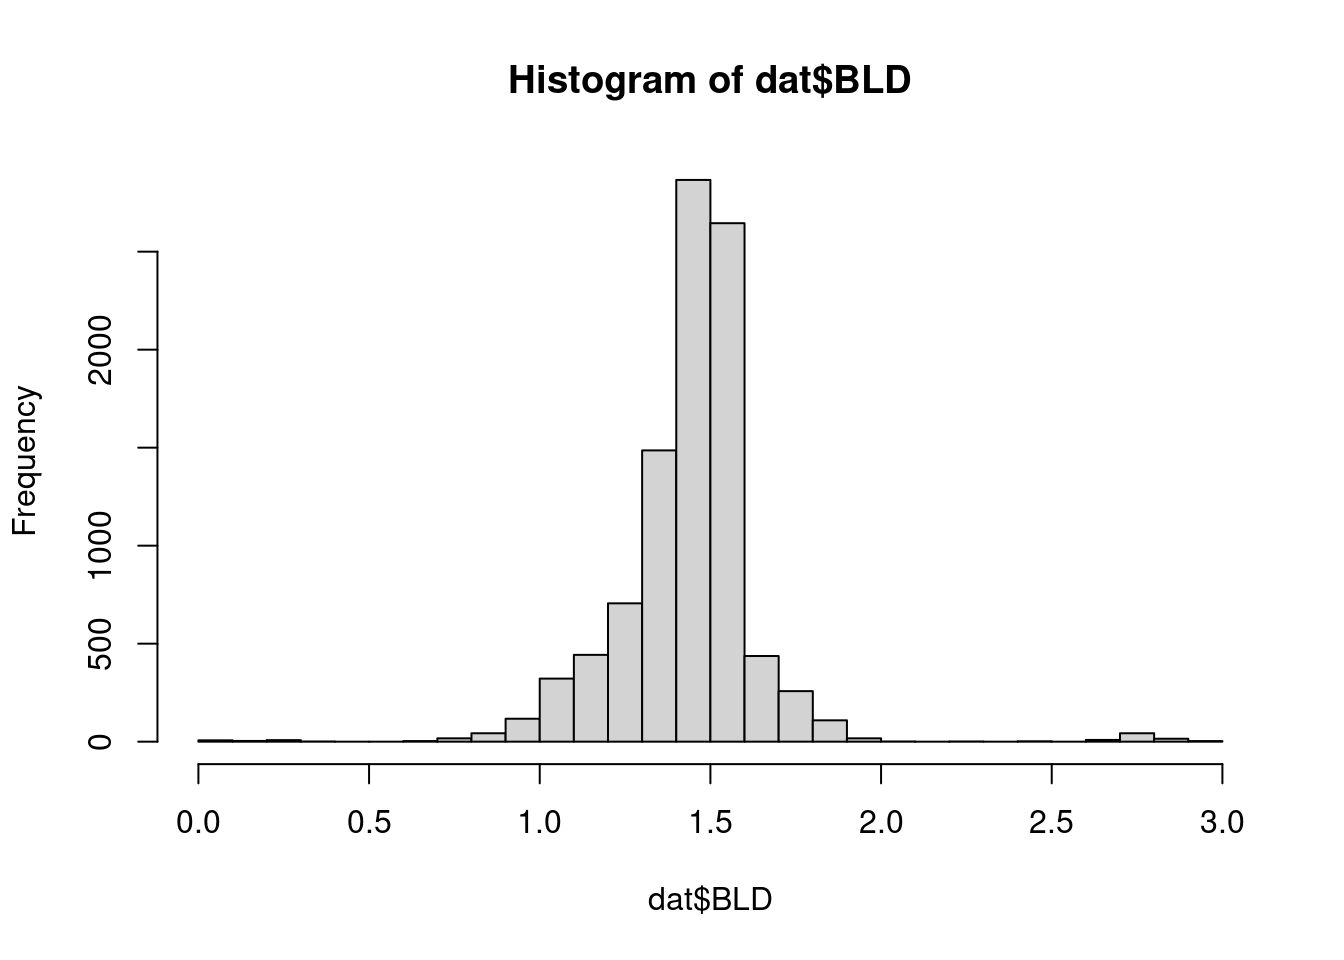
\includegraphics{SOCMapping_files/figure-latex/unnamed-chunk-5-1.pdf}
\caption{\label{fig:unnamed-chunk-5}Histogram of bulk density values}
\end{figure}

\hypertarget{soil-carbon-analysis}{%
\subsection{Soil Carbon Analysis}\label{soil-carbon-analysis}}

\cite{rosell2001soil} have closely reviewed the different SOC and SOM
estimation procedures, and have also drawn some conclusions about the
sources of errors. Determination of SOC from dry combustion methods is
least susceptible to errors.

\begin{itemize}
\item
  \textbf{Dry combustion by Loss on Ignition (LOI)}: SOC is
  re-calculated applying a conversion factor. It is commonly assumed,
  that organic matter contains an average of \(58\%\) organic carbon
  (so-called Van Bemmelen factor \(1.724\); for non-organic horizons:
  \(SOC = SOM / 1.724\)). For organic horizons, conversion factor ranges
  from \(1.9\) to \(2.5\) \citep{nelson1982total}. The inorganic carbon
  is not resolved, since typically, temperatures between 400°C and 550°C
  are used.
\item
  \textbf{Wet oxidation}: Since wet oxidation is applied without
  additional (external) heating, low temperatures of around 120°C
  (internal heat) are typical. Thus, the oxidation of carbon is
  incomplete, and a so-called oxidation factor needs to be applied. With
  external heating, the C-recovery of the method becomes improved, up to
  complete recovery. No correction of the mineral carbon is needed. Wet
  oxidation should typically only be applied to samples with \(<5\%\)
  organic matter.
\end{itemize}

Usually, an average of \(76\%\) organic carbon is recovered, leading to
a standard oxidation factor or \(1.33\) \citep{lettens2005soil}.

\hypertarget{carbonates}{%
\subsection{Carbonates}\label{carbonates}}

In case the total organic carbon is determined with temperatures higher
than 600°C to 800°C, the proportion of mineral soil in \(CaCO_3\) has to
be subtracted in order to derive the amount of organic carbon (inorganic
carbon is also oxidized). The pH value gives the first indication
whether the sample has to be analyzed for inorganic carbon or not.

It is crucial to report in the metadata whether national SOC values
refer to total C or if the inorganic component has been considered.

\hypertarget{depth}{%
\subsection{Depth}\label{depth}}

The standard depth for GSOCmap is \textbf{0 to 30 cm}. Subdivisions are
possible depending on the available data, by genetic horizons or depth
classes. The following depths are additionally considered for GSOCmap
(optional): * Forest floor: thickness (cm) subdivision in horizons
depending on national soil inventory method (e.g.~L, F, H) * Peat:
\textgreater{}30 , \textless{}100 depending on national data

\hypertarget{completeness-of-depth-estimate}{%
\section{Completeness of Depth
Estimate}\label{completeness-of-depth-estimate}}

Soil properties are commonly collected from field inventories (see Table
2.2) or from sampling and analyzing horizons and/or fixed depths. Since
a fixed target depth of 30 cm is required for GSOC (other depth classes
will be recommended in the future, following the \emph{GSP Guidelines
for Sharing National Data/Information to Compile a Global Soil Organic
Carbon (GSOC) Map}, data holders are confronted with the following
options:

\begin{itemize}
\tightlist
\item
  \textbf{Option 1}: Soil sampling has already considered this depth,
  data can be directly used for upscaling (see chapter
  \ref{mappingMethods}).
\item
  \textbf{Option 2}: Horizons or layers/depth classes are sampled but
  aggregation is needed over the 0 to 30 cm.
\item
  \textbf{Option 3}: The target depth (0 to 30 cm) was not completely
  covered by sampling, e.g.~only the A horizon or a topsoil layer
  (e.g.~0 to 20 cm) has been sampled.
\end{itemize}

For both \textbf{Options 2} and \textbf{3}, the transformation is
needed, using e.g.~equal-area splines. In the case of \textbf{Option 2},
the use of equal-area splines was first proposed by
\cite{ponce1986improved}, and later tested against real data
\citep{bishop1999modelling}. This technique is based on fitting
continuous depth functions for modeling the variability of soil
properties with depth. Thus, it is possible to convert soil profiles to
standard depths, but also to fill gaps. The equal-area spline function
consists of a series of local quadratic polynomials that join at
so-called knots, located at the horizon boundaries, whereby the mean
value of each horizon is maintained by the spline fit. They are called
equal-area splines because the area to the left of the fitted spline
curve is equal to the area to the right of the curve. In case of
\textbf{Option 3}, additional information on the vertical distribution
of carbon in the soils is required for accurate recalculation from the
sampling depth to target depth, e.g.~as was shown by
\cite{bernoux1998modeling}.

\hypertarget{EqualAreaSplines}{%
\subsection{Technical Steps - Equal-Area Splines Using
R}\label{EqualAreaSplines}}

In \textbf{R} environment, the easiest way to apply equal-area splines
is using the function \texttt{GSIF::mpspline} from the \textbf{R}
package \textbf{GSIF} (\cite{hengl_2016_gsif}, see section
\ref{SoilPedometrics}). For illustration, a sample dataset has been used
(see chapter \ref{covariates}). This function requires data stored as
\texttt{SoilProfileCollection} (SPC) using package \textbf{aqp}.
Nevertheless, data in any local soil database or in tables like the ones
proposed before (Tables @ref(tab:example table for site-level),
@ref(tab:example table for horizon-level)) can be transformed to an SPC.

The function \texttt{GSIF::mpspline} has several arguments. One of the
arguments is the lambda value mentioned before. The proposed default
value is 0.1. Another argument for this function is the target standard
depths. The function produces spline-estimated values at these depths.
However, this function also produces spline-estimated values at 1 cm
increments.

The following technical steps require \textbf{R} and the named packages.

\hypertarget{promote-table-dat-to-soilprofilecollection}{%
\subsubsection{\texorpdfstring{Promote table \texttt{dat} to
\texttt{SoilProfileCollection}}{Promote table dat to SoilProfileCollection}}\label{promote-table-dat-to-soilprofilecollection}}

\begin{Shaded}
\begin{Highlighting}[]
\CommentTok{# Load aqp package}
\KeywordTok{library}\NormalTok{(aqp)}

\CommentTok{# Promote to SoilProfileCollection }
\CommentTok{# The SoilProfileCollection is a object class in R designed to }
\CommentTok{# handle soil profiles}
\KeywordTok{depths}\NormalTok{(dat) <-}\StringTok{ }\NormalTok{ProfID }\OperatorTok{~}\StringTok{ }\NormalTok{top }\OperatorTok{+}\StringTok{ }\NormalTok{bottom}
\end{Highlighting}
\end{Shaded}

\begin{verbatim}
## Warning: converting IDs from factor to character
\end{verbatim}

\hypertarget{add-site-level-data-and-coordinates}{%
\subsubsection{Add site-level data and
coordinates}\label{add-site-level-data-and-coordinates}}

\begin{Shaded}
\begin{Highlighting}[]
\CommentTok{# Merge the soil horizons information with the site-level }
\CommentTok{# information from dat_sites}
\KeywordTok{site}\NormalTok{(dat) <-}\StringTok{ }\NormalTok{dat_sites}

\CommentTok{# Set spatial coordinates}
\KeywordTok{coordinates}\NormalTok{(dat) <-}\StringTok{ }\ErrorTok{~}\StringTok{ }\NormalTok{X }\OperatorTok{+}\StringTok{ }\NormalTok{Y}

\CommentTok{# A summary of our SoilProfileCollection}
\NormalTok{dat}
\end{Highlighting}
\end{Shaded}

\begin{verbatim}
## Object of class SoilProfileCollection
## Number of profiles: 4118
## Depth range: 5-295 cm
## 
## Horizon attributes:
##   ProfID    HorID top bottom SOC BLD CRF SAND SILT CLAY
## 1  P0000 P0000H01   4     23  NA  NA  54   52   34   14
## 2  P0000 P0000H02  23     46  NA  NA  62   59   31   11
## 3  P0000 P0000H03  46     59  NA  NA  47   67   24    8
## 4  P0001 P0001H01   2     11  NA  NA  66   45   39   16
## 5  P0001 P0001H02  11     31  NA  NA  70   40   31   28
## 6  P0002 P0002H01   0     22  NA  NA  57   52   33   15
## 
## Sampling site attributes:
##   ProfID X.1                                 soiltype Land.Cover
## 1  P0000   1                                 Cambisol         25
## 2  P0001   2                                 Cambisol         24
## 3  P0002   3                                 Cambisol         25
## 4  P0003   4                        Rendzic Leptosols         26
## 5  P0004   5                        Rendzic Leptosols         26
## 6  P0005   6 Complex of Rendzic Leptosol and Leptosol         27
## 
## Spatial Data:
##        min      max
## X 20.46434 23.01039
## Y 40.68543 42.35932
## [1] NA
\end{verbatim}

\hypertarget{run-mass-preserving-splines-for-all-the-needed-properties}{%
\subsubsection{Run mass preserving splines for all the needed
properties}\label{run-mass-preserving-splines-for-all-the-needed-properties}}

\begin{Shaded}
\begin{Highlighting}[]
\KeywordTok{library}\NormalTok{(GSIF)}

\NormalTok{## Estimate 0-30 standard horizon usin mass preserving splines}
\KeywordTok{try}\NormalTok{(SOC <-}\StringTok{ }\KeywordTok{mpspline}\NormalTok{(dat, }\StringTok{'SOC'}\NormalTok{, }\DataTypeTok{d =} \KeywordTok{t}\NormalTok{(}\KeywordTok{c}\NormalTok{(}\DecValTok{0}\NormalTok{,}\DecValTok{30}\NormalTok{))))}
\KeywordTok{try}\NormalTok{(BLD <-}\StringTok{ }\KeywordTok{mpspline}\NormalTok{(dat, }\StringTok{'BLD'}\NormalTok{, }\DataTypeTok{d =} \KeywordTok{t}\NormalTok{(}\KeywordTok{c}\NormalTok{(}\DecValTok{0}\NormalTok{,}\DecValTok{30}\NormalTok{))))}
\KeywordTok{try}\NormalTok{(CRFVOL <-}\StringTok{ }\KeywordTok{mpspline}\NormalTok{(dat, }\StringTok{'CRF'}\NormalTok{, }\DataTypeTok{d =} \KeywordTok{t}\NormalTok{(}\KeywordTok{c}\NormalTok{(}\DecValTok{0}\NormalTok{,}\DecValTok{30}\NormalTok{))))}
\end{Highlighting}
\end{Shaded}

\hypertarget{convert-back-to-table}{%
\subsubsection{Convert back to table}\label{convert-back-to-table}}

\begin{Shaded}
\begin{Highlighting}[]
\NormalTok{## Prepare final data frame}
\NormalTok{dat <-}\StringTok{ }\KeywordTok{data.frame}\NormalTok{(}\DataTypeTok{id =}\NormalTok{ dat}\OperatorTok{@}\NormalTok{site}\OperatorTok{$}\NormalTok{ProfID,}
                  \DataTypeTok{Y =}\NormalTok{ dat}\OperatorTok{@}\NormalTok{sp}\OperatorTok{@}\NormalTok{coords[,}\DecValTok{2}\NormalTok{],}
                  \DataTypeTok{X =}\NormalTok{ dat}\OperatorTok{@}\NormalTok{sp}\OperatorTok{@}\NormalTok{coords[,}\DecValTok{1}\NormalTok{],}
                  \DataTypeTok{SOC =}\NormalTok{ SOC}\OperatorTok{$}\NormalTok{var.std[,}\DecValTok{1}\NormalTok{],}
                  \DataTypeTok{BLD =}\NormalTok{ BLD}\OperatorTok{$}\NormalTok{var.std[,}\DecValTok{1}\NormalTok{],}
                  \DataTypeTok{CRFVOL =}\NormalTok{ CRFVOL}\OperatorTok{$}\NormalTok{var.std[,}\DecValTok{1}\NormalTok{])}

\NormalTok{dat <-}\StringTok{ }\NormalTok{dat[}\KeywordTok{complete.cases}\NormalTok{(dat),]}

\NormalTok{## Take a look at the results}
\KeywordTok{head}\NormalTok{(dat)}
\end{Highlighting}
\end{Shaded}

\begin{verbatim}
##       id        Y        X       SOC       BLD    CRFVOL
## 4  P0003 42.02828 20.81819 26.380000 0.7304483  8.000000
## 5  P0004 42.02747 20.81464 24.561667 0.8955320  6.305316
## 7  P0006 42.02885 20.82757 19.940000 0.7886235 14.000000
## 8  P0007 42.02279 20.83165  6.149114 1.1653355 18.633590
## 9  P0008 42.05014 20.82036  3.940352 1.2962582 31.875748
## 10 P0009 42.02047 20.93529  3.258545 1.3446297 21.714059
\end{verbatim}

\hypertarget{estimate-the-soil-organic-carbon-stock-using-the-virtual-horizons}{%
\subsubsection{Estimate the soil organic carbon stock using the virtual
horizons}\label{estimate-the-soil-organic-carbon-stock-using-the-virtual-horizons}}

Finally, the estimation of the soil organic carbon stock (OKS) can be
done using the \textbf{GSIF} package.

\begin{Shaded}
\begin{Highlighting}[]
\KeywordTok{library}\NormalTok{(GSIF)}
\CommentTok{# Estimate Organic Carbon Stock}
\CommentTok{# SOC must be in g/kg}
\CommentTok{# BLD in kg/m3}
\CommentTok{# CRF in percentage}
\NormalTok{OCSKGM <-}\StringTok{ }\KeywordTok{OCSKGM}\NormalTok{(}\DataTypeTok{ORCDRC =}\NormalTok{ dat}\OperatorTok{$}\NormalTok{SOC, }\DataTypeTok{BLD =}\NormalTok{ dat}\OperatorTok{$}\NormalTok{BLD}\OperatorTok{*}\DecValTok{1000}\NormalTok{, }
                 \DataTypeTok{CRFVOL =}\NormalTok{ dat}\OperatorTok{$}\NormalTok{CRFVOL, }\DataTypeTok{HSIZE =} \DecValTok{30}\NormalTok{)}

\NormalTok{dat}\OperatorTok{$}\NormalTok{OCSKGM <-}\StringTok{ }\NormalTok{OCSKGM}
\NormalTok{dat}\OperatorTok{$}\NormalTok{meaERROR <-}\StringTok{ }\KeywordTok{attr}\NormalTok{(OCSKGM,}\StringTok{"measurementError"}\NormalTok{)}
\NormalTok{dat <-}\StringTok{ }\NormalTok{dat[dat}\OperatorTok{$}\NormalTok{OCSKGM}\OperatorTok{>}\DecValTok{0}\NormalTok{,]}
\KeywordTok{summary}\NormalTok{(dat)}
\end{Highlighting}
\end{Shaded}

\begin{verbatim}
##        id             Y               X              SOC        
##  P0003  :   1   Min.   :40.69   Min.   :20.46   Min.   : 0.080  
##  P0004  :   1   1st Qu.:41.19   1st Qu.:21.35   1st Qu.: 1.750  
##  P0006  :   1   Median :41.42   Median :21.49   Median : 2.603  
##  P0007  :   1   Mean   :41.49   Mean   :21.66   Mean   : 3.539  
##  P0008  :   1   3rd Qu.:41.83   3rd Qu.:22.14   3rd Qu.: 4.089  
##  P0009  :   1   Max.   :42.36   Max.   :23.01   Max.   :86.510  
##  (Other):3880                                                   
##       BLD              CRFVOL             OCSKGM      
##  Min.   :0.05353   Min.   : 0.00000   Min.   :0.0111  
##  1st Qu.:1.28089   1st Qu.: 0.00516   1st Qu.:0.6951  
##  Median :1.39549   Median : 5.01397   Median :0.9866  
##  Mean   :1.38073   Mean   :11.02257   Mean   :1.1399  
##  3rd Qu.:1.47612   3rd Qu.:17.69065   3rd Qu.:1.3997  
##  Max.   :2.92191   Max.   :93.95013   Max.   :7.4302  
##                                                       
##     meaERROR    
##  Min.   :0.172  
##  1st Qu.:3.160  
##  Median :3.840  
##  Mean   :3.715  
##  3rd Qu.:4.260  
##  Max.   :8.770  
## 
\end{verbatim}

Soil organic carbon tends to have a log-normal distribution with a
right-skew, and transforming the original values to its natural
logarithm would generate a normal distribution of soil organic carbon
values. Here we will test if the log transformation of the response
variable (\emph{SOC}) tends to normality and 2) if this transformation
increases the simple correlation of \emph{SOC} and its prediction
factors.

\begin{Shaded}
\begin{Highlighting}[]
\CommentTok{# Generate a new column with the transformed OCSKGM to its natural }
\CommentTok{# logarithm}
\NormalTok{dat}\OperatorTok{$}\NormalTok{OCSKGMlog <-}\StringTok{ }\KeywordTok{log}\NormalTok{(dat}\OperatorTok{$}\NormalTok{OCSKGM)}

\NormalTok{## plot the next two plots as one}
\KeywordTok{par}\NormalTok{(}\DataTypeTok{mfrow=}\KeywordTok{c}\NormalTok{(}\DecValTok{1}\NormalTok{,}\DecValTok{2}\NormalTok{))}
\KeywordTok{plot}\NormalTok{(}\KeywordTok{density}\NormalTok{(dat}\OperatorTok{$}\NormalTok{OCSKGM),}
     \DataTypeTok{main=}\StringTok{'original values'}\NormalTok{)}

\KeywordTok{plot}\NormalTok{(}\KeywordTok{density}\NormalTok{(dat}\OperatorTok{$}\NormalTok{OCSKGMlog),}
     \DataTypeTok{main=}\StringTok{'log transformed values'}\NormalTok{)}
\end{Highlighting}
\end{Shaded}

\begin{figure}
\centering
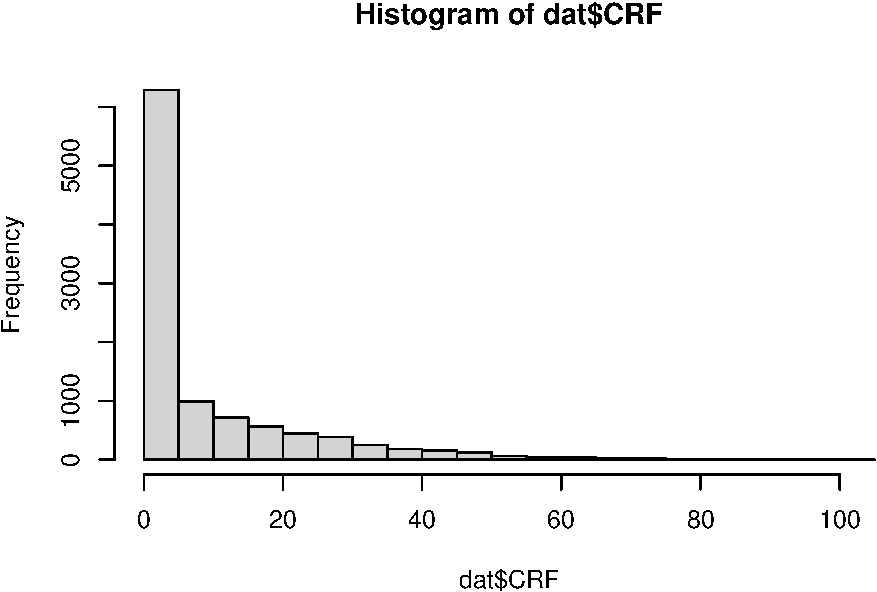
\includegraphics{SOCMapping_files/figure-latex/unnamed-chunk-9-1.pdf}
\caption{\label{fig:unnamed-chunk-9}Statistical distribution of original OCS
values vs log-transformed values}
\end{figure}

\begin{Shaded}
\begin{Highlighting}[]
\KeywordTok{par}\NormalTok{(}\DataTypeTok{mfrow=}\KeywordTok{c}\NormalTok{(}\DecValTok{1}\NormalTok{,}\DecValTok{1}\NormalTok{))}

\NormalTok{## We can save our processed data as a table}
\KeywordTok{write.csv}\NormalTok{(dat, }\StringTok{"data/dataproc.csv"}\NormalTok{, }\DataTypeTok{row.names =} \OtherTok{FALSE}\NormalTok{)}
\end{Highlighting}
\end{Shaded}

\hypertarget{setting-up-the-software-environment}{%
\chapter{Setting-Up the Software
Environment}\label{setting-up-the-software-environment}}

\emph{Y Yigini}

This cookbook focuses on SOC modeling using open source digital mapping
tools. The instructions and screen-captures in this section will guide
you through installing and manually configuring the software to be used
for digital soil mapping procedures for \emph{Microsoft Windows} desktop
platform. Instructions for the other platforms (e.g. \emph{Linux
Flavours}, \emph{MacOS}) can be found through free online resources.

\hypertarget{use-of-r-rstudio-and-r-packages}{%
\section{Use of R, RStudio and R
Packages}\label{use-of-r-rstudio-and-r-packages}}

\textbf{R} is a language and environment for statistical computing. It
provides a wide variety of statistical (e.g.~linear modeling,
statistical tests, time-series, classification, clustering, etc.) and
graphical methods, and is highly extensible.

\hypertarget{obtaining-and-installing-r}{%
\subsection{Obtaining and Installing
R}\label{obtaining-and-installing-r}}

\begin{itemize}
\tightlist
\item
  Go to \url{https://cloud.r-project.org/index.html} to download and
  install \textbf{R}.
\item
  Pick an installation file for your platform.
\end{itemize}

\hypertarget{obtaining-and-installing-r-studio}{%
\subsection{Obtaining and Installing R
Studio}\label{obtaining-and-installing-r-studio}}

Beginners will find it very hard to start using \textbf{R} because it
has no Graphical User Interface (GUI). There are some GUIs which offer
some of the functionality of \textbf{R}. \textbf{RStudio} makes
\textbf{R} easier to use. It includes a code editor, debugging and
visualization tools, therefore, in this cookbook we would like to focus
on the latter including a GUI. You can follow very similar steps to
install \textbf{RStudio}.

\begin{itemize}
\tightlist
\item
  Go to \url{https://www.rstudio.com/products/rstudio/download/} to
  download and install \textbf{RStudio}'s open source edition.
\item
  On the download page, \emph{RStudio Desktop, Open Source License}
  option should be selected.
\item
  Pick an installation file for your platform.
\end{itemize}

\hypertarget{getting-started-with-r}{%
\subsection{Getting Started with R}\label{getting-started-with-r}}

\begin{itemize}
\tightlist
\item
  \textbf{R} Manuals: \url{http://cran.r-project.org/manuals.html}
\item
  Contributed Documentation:
  \url{http://cran.r-project.org/other-docs.html}
\item
  Quick-\textbf{R}: \url{http://www.statmethods.net/index.html}
\item
  Stackoverflow \textbf{R} Community:
  \url{https://stackoverflow.com/questions/tagged/r}
\end{itemize}

\hypertarget{r-packages}{%
\section{R Packages}\label{r-packages}}

When you download \textbf{R}, you get the basic \textbf{R} system which
implements the \textbf{R} language. \textbf{R} becomes more useful with
the large collection of packages that extend the basic functionality of
it. \textbf{R} packages are developed by the \textbf{R} community.

\hypertarget{finding-r-packages}{%
\subsection{Finding R Packages}\label{finding-r-packages}}

The primary source for \textbf{R} packages is
\href{https://cran.r-project.org/}{\emph{CRAN}'s} official website,
where currently about 12.000 available packages are listed. For spatial
applications, various packages are available. You can obtain information
about the available packages directly on \emph{CRAN} with the
\texttt{available.packages()} function. The function returns a matrix of
details corresponding to packages currently available at one or more
repositories. An easier way to browse the list of packages is using the
\href{https://cran.r-project.org/web/views/}{\emph{Task Views}} link,
which groups together packages related to a given topic.

\hypertarget{most-used-r-packages-for-digital-soil-mapping}{%
\subsection{Most Used R Packages for Digital Soil
Mapping}\label{most-used-r-packages-for-digital-soil-mapping}}

As was previously mentioned, \textbf{R} is extensible through packages.
\textbf{R} packages are collections of \textbf{R} functions, data,
documentation and compiled code easy to share with others. In the
following subsections, we are going to present the most used packages
related to digital soil property mapping.

\hypertarget{SoilPedometrics}{%
\subsubsection{Soil Science and Pedometrics}\label{SoilPedometrics}}

\href{https://CRAN.R-project.org/package=aqp}{\textbf{aqp}}: Algorithms
for quantitative pedology. A collection of algorithms related to
modeling of soil resources, soil classification, soil profile
aggregation, and visualization.

\href{https://CRAN.R-project.org/package=GSIF}{\textbf{GSIF}}: Global
Soil Information Facility (GSIF). Tools, functions and sample datasets
for digital soil mapping. GSIF tools (standards and functions) and
sample datasets for global soil mapping.

\href{http://ithir.r-forge.r-project.org/}{\textbf{ithir}}: A collection
of functions and algorithms specific to pedometrics. The package was
developed by Brendan Malone at the University of Sydney.

\href{https://CRAN.R-project.org/package=soiltexture}{\textbf{soiltexture}}:
The
\href{https://cran.r-project.org/web/packages/soiltexture/vignettes/soiltexture_vignette.pdf}{\emph{Soil
Texture Wizard}} is a set of \textbf{R} functions designed to produce
texture triangles (also called texture plots, texture diagrams, texture
ternary plots), classify and transform soil textures data. These
functions virtually allow to plot any soil texture triangle
(classification) into any triangle geometry (isosceles, right-angled
triangles, etc.). The set of functions is expected to be useful to
people using soil textures data from different soil texture
classification or different particle size systems. Many (\textgreater{}
15) texture triangles from all around the world are predefined in the
package. A simple text-based GUI is provided:
\texttt{soiltexture\_gui()}.

\hypertarget{spatial-analysis}{%
\subsubsection{Spatial Analysis}\label{spatial-analysis}}

\href{https://CRAN.R-project.org/package=sp}{\textbf{sp}}: The package
provides classes and methods for spatial data. The classes document
where the spatial location information resides, for 2D or 3D data.

\href{https://CRAN.R-project.org/package=raster}{\textbf{raster}}:
Reading, writing, manipulating, analyzing and modeling of gridded
spatial data. The package implements basic and high-level functions,
processing of very large files is supported.

\href{https://CRAN.R-project.org/package=rgdal}{\textbf{rgdal}}:
Provides bindings to Frank Warmerdam's Geospatial Data Abstraction
Library (GDAL).

\href{https://CRAN.R-project.org/package=RSAGA}{\textbf{RSAGA}}: The
package provides access to geocomputing and terrain analysis functions
of \href{/url\%7Bhttp://www.saga-gis.org/en/index.html\%7D}{\emph{SAGA
GIS}} from within \textbf{R} by running the command line version of
\emph{SAGA}.

\hypertarget{modeling}{%
\subsubsection{Modeling}\label{modeling}}

\href{https://CRAN.R-project.org/package=caret}{\textbf{caret}}:
Extensive range of functions for training and plotting classification
and regression models.

\href{https://CRAN.R-project.org/package=Cubist}{\textbf{Cubist}}:
Regression modeling using rules with added instance-based corrections.
Cubist models were developed by Ross Quinlan.

\href{https://CRAN.R-project.org/package=C5.0}{\textbf{C5.0}}: C5.0
decision trees and rule-based models for pattern recognition. Another
model structure developed by Ross Quinlan.

\href{https://CRAN.R-project.org/package=gam}{\textbf{gam}}: Functions
for fitting and working with generalized additive models.

\href{https://CRAN.R-project.org/package=nnet}{\textbf{nnet}}: Software
for feed-forward neural networks with a single hidden layer, and for
multinomial log-linear models.

\href{https://CRAN.R-project.org/package=gstat}{\textbf{gstat}}:
Variogram modeling with simple, ordinary and universal point or block
(co)kriging, sequential Gaussian or indicator (co)simulation. The
package includes variogram and variogram map plotting utility functions.

\href{https://CRAN.R-project.org/package=automap}{\textbf{automap}}:
This package performs an automatic interpolation by automatically
estimating the variogram and then calling
\href{https://CRAN.R-project.org/package=gstat}{\textbf{gstat}}.

\hypertarget{mapping-and-plotting}{%
\subsubsection{Mapping and Plotting}\label{mapping-and-plotting}}

Both \textbf{raster} and \textbf{sp} have handy functions for plotting
spatial data. Besides using the base plotting functionality, another
useful plotting package is
\href{https://cran.r-project.org/web/packages/ggplot2/index.html}{\textbf{ggplot2}}.

\href{https://CRAN.R-project.org/package=plotKML}{\textbf{plotKML}}:
Writes sp-class, spacetime-class, raster-class and similar spatial and
spatiotemporal objects to KML following some basic cartographic rules.

\href{https://CRAN.R-project.org/package=leaflet}{\textbf{leaflet}}:
Create and customize interactive maps using the Leaflet JavaScript
library and the
\href{https://cran.r-project.org/web/packages/htmlwidgets/index.html}{\textbf{htmlwidgets}}
package. These maps can be used directly from the \textbf{R} console,
from \textbf{RStudio}, in
\href{https://shiny.rstudio.com/}{\textbf{Shiny}} apps and
\textbf{RMarkdown} documents.

\hypertarget{r-and-spatial-data}{%
\section{R and Spatial Data}\label{r-and-spatial-data}}

\textbf{R} has a large and growing number of spatial data packages. We
recommend taking a quick browse on \textbf{R}'s official website to see
the spatial packages available:
\url{http://cran.r-project.org/web/views/Spatial.html}

\hypertarget{reading-shapefiles}{%
\subsection{Reading Shapefiles}\label{reading-shapefiles}}

\emph{ESRI}'s shapefile format is widely used for storing vector-based
spatial data (i.e., points, lines, polygons). This example demonstrates
use of raster package that provides functions for reading and/or writing
shapefiles.

\begin{Shaded}
\begin{Highlighting}[]
\KeywordTok{library}\NormalTok{(raster)}
\CommentTok{# load the soil map from a shapefile file}
\NormalTok{soilmap <-}\StringTok{ }\KeywordTok{shapefile}\NormalTok{(}\StringTok{"MK_soilmap_simple.shp"}\NormalTok{)}
\end{Highlighting}
\end{Shaded}

We may want to use these data in other GIS environments such as
\emph{ArcGIS}, \emph{QGIS}, \emph{SAGA GIS}, etc. This means we need to
export the \texttt{SpatialPointsDataFrame} to an appropriate spatial
data format such as a shapefile.

\begin{Shaded}
\begin{Highlighting}[]
\CommentTok{# For example, we can select the soil units classified as }
\CommentTok{# Fluvisols according to WRB}
\NormalTok{Fluvisols <-}\StringTok{ }\NormalTok{soilmap[soilmap}\OperatorTok{$}\NormalTok{WRB }\OperatorTok{==}\StringTok{ "Fluvisol"}\NormalTok{,]}

\CommentTok{# and save this as a new shapefile }
\KeywordTok{shapefile}\NormalTok{(Fluvisols, }\DataTypeTok{filename =} \StringTok{'results/fluvisols.shp'}\NormalTok{,}
          \DataTypeTok{overwrite =} \OtherTok{TRUE}\NormalTok{)}
\end{Highlighting}
\end{Shaded}

\hypertarget{coordinate-reference-systems-crs-in-r}{%
\subsection{Coordinate Reference Systems (CRS) in
R}\label{coordinate-reference-systems-crs-in-r}}

We need to define the CRS (Coordinate Reference System) to be able to
perform any sort of spatial analysis in \textbf{R}. To clearly tell
\textbf{R} this information we define the CRS which describes a
reference system in a way understood by the PROJ.4 projection library
\url{http://trac.osgeo.org/proj/}.

An interface to the PROJ.4 library is available in the \textbf{rgdal}
package. An alternative to using Proj4 character strings, we can use the
corresponding yet simpler EPSG (European Petroleum Survey Group) code.
\textbf{rgdal} also recognizes these codes. If you are unsure of the
Proj4 or EPSG code for the spatial data that you have but know the CRS,
you should consult \url{http://spatialreference.org/} for assistance.

\begin{Shaded}
\begin{Highlighting}[]
\NormalTok{## print the CRS for the object soilmap}
\NormalTok{soilmap}\OperatorTok{@}\NormalTok{proj4string}
\end{Highlighting}
\end{Shaded}

\begin{verbatim}
## CRS arguments:
##  +proj=longlat +datum=WGS84 +no_defs +ellps=WGS84
## +towgs84=0,0,0
\end{verbatim}

The following example shows how you can create a spatial object from a
.csv file. We can use the \texttt{coordinates()} function from the
\textbf{sp} package to define which columns in the data frame refer to
actual spatial coordinates---here the coordinates are listed in columns
X and Y.

\begin{Shaded}
\begin{Highlighting}[]
\CommentTok{# load the table with the soil observations site information}
\NormalTok{dat_sites <-}\StringTok{ }\KeywordTok{read.csv}\NormalTok{(}\DataTypeTok{file =} \StringTok{"data/site-level.csv"}\NormalTok{)}

\CommentTok{# convert from table to spatial points object}
\KeywordTok{coordinates}\NormalTok{(dat_sites) <-}\StringTok{ }\ErrorTok{~}\StringTok{ }\NormalTok{X }\OperatorTok{+}\StringTok{ }\NormalTok{Y}

\CommentTok{# check the coordinate system:}
\NormalTok{dat_sites}\OperatorTok{@}\NormalTok{proj4string}
\end{Highlighting}
\end{Shaded}

\begin{verbatim}
## CRS arguments: NA
\end{verbatim}

\begin{Shaded}
\begin{Highlighting}[]
\CommentTok{# as the CRS is not defined, we can assign the correct CRS is we}
\CommentTok{# have information about it. In this case, it should be EPSG:4326}
\NormalTok{dat_sites}\OperatorTok{@}\NormalTok{proj4string <-}\StringTok{ }\KeywordTok{CRS}\NormalTok{(}\StringTok{"+init=epsg:4326"}\NormalTok{)}

\CommentTok{# check the CRS again:}
\NormalTok{dat_sites}\OperatorTok{@}\NormalTok{proj4string}
\end{Highlighting}
\end{Shaded}

\begin{verbatim}
## CRS arguments:
##  +init=epsg:4326 +proj=longlat +datum=WGS84 +no_defs
## +ellps=WGS84 +towgs84=0,0,0
\end{verbatim}

\hypertarget{working-with-rasters}{%
\subsection{Working with Rasters}\label{working-with-rasters}}

Most of the functions for handling raster data are available in the
\textbf{raster} package. There are functions for reading and writing
raster files from and to different formats. In digital soil mapping, we
mostly work with data in table format and then rasterize this data so
that we can produce a continuous map. For doing this in \textbf{R}
environment, we will load raster data in a data frame. This data is a
digital elevation model (DEM) provided by
\href{http://www.isric.org/}{\emph{ISRIC}} for Former Yugoslav Republic
of Macedonia (FYROM).

\begin{Shaded}
\begin{Highlighting}[]
\CommentTok{#For handling raster data, we load raster package}
\KeywordTok{library}\NormalTok{(raster)}

\CommentTok{#load DEM from tif file}
\NormalTok{DEM <-}\StringTok{ }\KeywordTok{raster}\NormalTok{(}\StringTok{"covs/DEMENV5.tif"}\NormalTok{)}
\end{Highlighting}
\end{Shaded}

We may want to export this raster to a suitable format to work in a
standard GIS environment. See the help file for writing a raster
\texttt{?writeRaster} to get information regarding the supported grid
types that data can be exported into. Here, we will export our raster to
\emph{ESRI} Ascii, as it is a common and universal raster format.

We may also want to export our mac.dem to KML file using the
\texttt{KML()} function. \texttt{KML()} is a handy function from the
\textbf{raster} package for exporting grids to kml format. Note that we
need to re-project the data to WGS84 geographic. The raster
re-projection is performed using the \texttt{projectRaster()} function.
Look at the help file \texttt{?projectRaster} for this.

\hypertarget{other-dsm-related-software-and-tools}{%
\section{Other DSM Related Software and
Tools}\label{other-dsm-related-software-and-tools}}

\begin{itemize}
\tightlist
\item
  \emph{QGIS}: Available at
  \url{http://www.qgis.org/en/site/forusers/download.html}
\item
  \emph{SAGA GIS}: Available at
  \url{https://sourceforge.net/projects/saga-gis/files/}
\end{itemize}

\hypertarget{covariates}{%
\chapter{Preparation of Spatial covariates}\label{covariates}}

\emph{R Baritz \& Y Yigini}

The example covariates from this chapter were prepared by \emph{ISRIC}.
The access and use limitations are presented in section
\ref{GSOCDataRepo}. A small subset of these covariates, comprising most
of the soil forming factors, will be used for the examples. This subset
is presented in the following table.

\begin{table}

\caption{\label{tab:covariates}Code and name of example covariates provided with the cookbook.}
\centering
\begin{tabular}[t]{ll}
\toprule
CODE & ATTRIBUTE\_TITLE\\
\midrule
DEMENV5 & Land surface elevation\\
SLPMRG5 & Terrain slope\\
VBFMRG5 & Multiresolution Index of Valley Bottom Flatness (MRVBF)\\
VDPMRG5 & Valley depth\\
TWIMRG5 & SAGA Wetness Index\\
\addlinespace
TMDMOD3 & Mean annual LST (daytime) MODIS\\
TMNMOD3 & Mean annual LST (nighttime) MODIS\\
PRSCHE3 & Total annual precipitation at 1 km\\
B04CHE3 & Temperature seasonality at 1 km\\
B07CHE3 & Temperature Annual Range at 1 km\\
\addlinespace
B13CHE3 & Precipitation of wettest month [mm]\\
B14CHE3 & Precipitation of driest month [mm] at 1 km\\
LCEE10 & ESA land cover map 2010\\
\bottomrule
\end{tabular}
\end{table}

\hypertarget{dem-derived-covariates}{%
\section{DEM-Derived Covariates}\label{dem-derived-covariates}}

\hypertarget{dem-source-data-sets}{%
\subsection{DEM Source Data Sets}\label{dem-source-data-sets}}

Currently, two global level 30 m DEMs are freely available: the Shuttle
Radar Topographic Mission (SRTM) and the ASTER Global Digital Elevation
Model (GDEM). They provide topographic data at the global scale, which
are freely available for users. Both DEMs were compared by
\citet{Wong2014}. Comparison against high-resolution topographic data of
Light Detection and Ranging (LiDAR) in a mountainous tropical montane
landscape showed that the SRTM (90 m) produced better topographic data
in comparison with ASTER GDEM.

\begin{quote}
\begin{itemize}
\tightlist
\item
  Recommended for national level applications: 30 m GDEM / SRTM.
\item
  Recommended for global level applications: SRTM 90 m, resampled 1
  kilometer.
\end{itemize}
\end{quote}

In both cases, noise and artefacts need to be filtered out. ASTER seems
to contain more large artifacts (e.g.~peaks), particularly in flat
terrain, which are very difficult to remove through filtering.

\begin{Shaded}
\begin{Highlighting}[]
\CommentTok{#For handling raster data, we load raster package}
\KeywordTok{library}\NormalTok{(raster)}

\CommentTok{#load DEM from tif file}
\NormalTok{DEM <-}\StringTok{ }\KeywordTok{raster}\NormalTok{(}\StringTok{"covs/DEMENV5.tif"}\NormalTok{)}
\KeywordTok{plot}\NormalTok{(DEM)}
\end{Highlighting}
\end{Shaded}

\begin{figure}
\centering
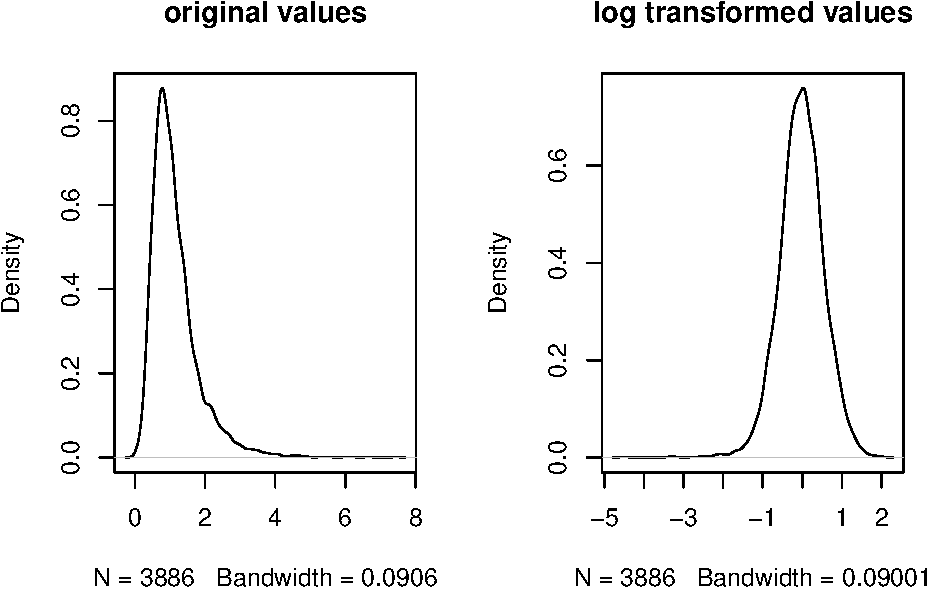
\includegraphics{SOCMapping_files/figure-latex/unnamed-chunk-15-1.pdf}
\caption{\label{fig:unnamed-chunk-15}SRTM 90m, resampled to 1km for FYROM}
\end{figure}

\begin{quote}
\emph{GRASS GIS} or GDAL: Use ``mdenoise'' module/utility to remove
noise while preserving sharp features like ridges, lines, and valleys.
\end{quote}

SRTM contains many gaps (pixels with no-data). These gaps could be
filled using splines. SAGA GIS has a module called `Close Gaps with
Splines' and other similar tools for doing this.

\hypertarget{parent-material}{%
\section{Parent Material}\label{parent-material}}

Parent material has a crucial impact on soil formation, soil
geochemistry, and soil physics. Parent material, if not specifically
mapped by soil mappers and included in soil maps, is usually available
from geological maps. These maps focus on rock formation, mineral
components, and age, and often lack younger surface sediments (even in
quaternary maps). Parent material/rock types classified by soil mappers
considers more strongly geochemistry and rock structure. Its
geochemistry has an essential impact on the soil chemistry, e.g.~cation
exchange capacity, base saturation, and nutrient stock. The rock
structure determines the ability to disintegrate, which has an impact on
soil physical properties, like texture, skeleton content, permeability,
and soil thickness.

National parent material and geological maps may be used. Other
available datasets and data portals are given on the \emph{ISRIC}
\href{http://worldgrids.org/doku.php}{WorldGrids} website.

\begin{itemize}
\item
  OneGeology: The world geological maps are now being integrated via the
  OneGeology project which aims at producing a consistent geological map
  of the world in approximate scale 1:1M \citep{jackson2007onegeology};
  Link: \url{http://www.onegeology.org/}.
\item
  \emph{USGS} has several data portals, e.g.~that allows browsing of the
  International Surface Geology (split into South Asia, South America,
  Iran, Gulf of Mexico, Former Soviet Union, Europe, Caribbean,
  Bangladesh, Asia Pacific, Arctic, Arabian Peninsula, Africa and
  Afghanistan); Link: \url{https://mrdata.usgs.gov/geology/world/}.
\item
  \citet{hartmann2012new} have assembled a global, purely lithological
  database called GLiM (Global Lithological Map). GLiM consists of over
  1.25 million digital polygons that are classified into three levels (a
  total of 42 rock-type classes); Link:
  \url{https://www.geo.uni-hamburg.de/en/geologie/forschung/geochemie/glim.html}).
\item
  \emph{USGS} jointly with \emph{ESRI} has released in 2014 a Global
  Ecological Land Units map at 250 m resolution. This also includes
  world layer of rock types. This data can be downloaded from the USGS
  site (\url{http://rmgsc.cr.usgs.gov/outgoing/ecosystems/Global/}).
\end{itemize}

\hypertarget{soil-maps}{%
\section{Soil Maps}\label{soil-maps}}

Soil maps play a crucial role for upscaling soil property data from
point locations. They can be the spatial layer for conventional
upscaling, they can also serve as a covariate in digital soil mapping.
Predicted soil property maps have lower quality in areas where the
covariates such as relief, geology, and climate do not correlate well
with the dependent variable, here SOC stocks. This is especially true
for soils under groundwater or stagnic water influence. This information
is well-represented in soil maps.

FAO, IIASA, ISRIC, ISS CAS and JRC produced a gridded 1 km soil class
map (HWSD). Global HWSD-derived soil property maps can be downloaded as
geotiffs at
\url{http://worldgrids.org/doku.php/wiki:layers\#harmonized_world_soil_database_images_5_km}
(see section \ref{GSOCDataRepo}).

\begin{Shaded}
\begin{Highlighting}[]
\CommentTok{# load the soil map from a shapefile file}
\NormalTok{soilmap <-}\StringTok{ }\KeywordTok{shapefile}\NormalTok{(}\StringTok{"MK_soilmap_simple.shp"}\NormalTok{)}

\CommentTok{# plot the DEM together with the soil types}
\KeywordTok{plot}\NormalTok{(DEM)}
\KeywordTok{lines}\NormalTok{(soilmap)}
\end{Highlighting}
\end{Shaded}

\begin{figure}
\centering
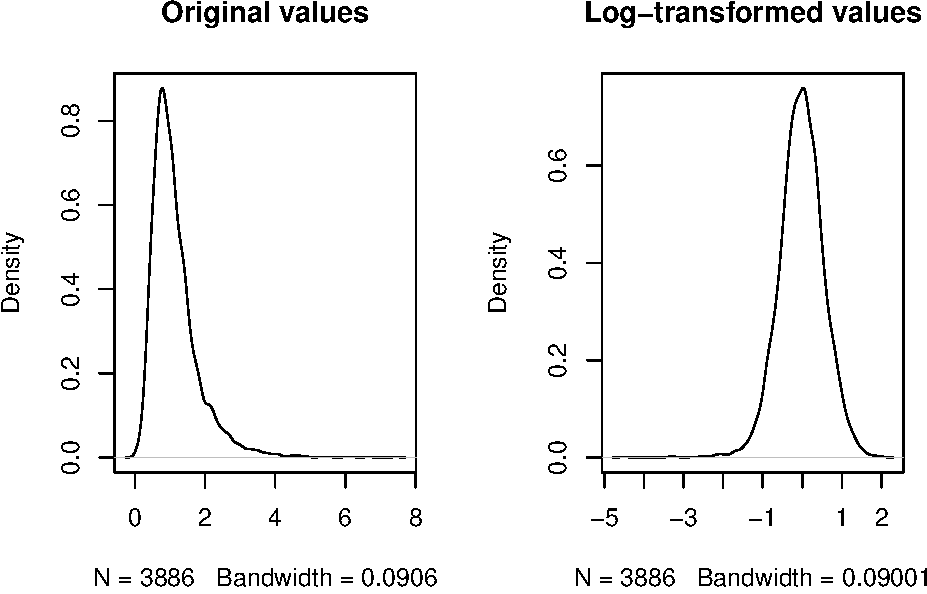
\includegraphics{SOCMapping_files/figure-latex/unnamed-chunk-16-1.pdf}
\caption{\label{fig:unnamed-chunk-16}soil map of MK}
\end{figure}

\begin{quote}
Digitized small-scale national soil maps are the most important spatial
layer for soil property mapping. The higher its resolution, the better
soil maps contribute to high-quality soil property maps - considering
that the map should cover the target area/full country coverage.
\end{quote}

\hypertarget{technical-steps---rasterizing-a-vector-layer-in-r}{%
\subsection{Technical Steps - Rasterizing a Vector Layer in
R}\label{technical-steps---rasterizing-a-vector-layer-in-r}}

\begin{Shaded}
\begin{Highlighting}[]
\CommentTok{# the "Symbol" attribute from the vector layer will be used for the}
\CommentTok{# rasterization process. It has to be a factor}
\NormalTok{soilmap}\OperatorTok{@}\NormalTok{data}\OperatorTok{$}\NormalTok{Symbol <-}\StringTok{ }\KeywordTok{as.factor}\NormalTok{(soilmap}\OperatorTok{@}\NormalTok{data}\OperatorTok{$}\NormalTok{Symbol)}

\CommentTok{#save the levels names in a character vector}
\NormalTok{Symbol.levels <-}\StringTok{ }\KeywordTok{levels}\NormalTok{(soilmap}\OperatorTok{$}\NormalTok{Symbol)}

\CommentTok{# The rasterization process needs a layer with the target grd }
\CommentTok{# system: spatial extent and cell size.}
\NormalTok{soilmap.r <-}\StringTok{ }\KeywordTok{rasterize}\NormalTok{(}\DataTypeTok{x =}\NormalTok{ soilmap, }\DataTypeTok{y =}\NormalTok{ DEM, }\DataTypeTok{field =} \StringTok{"Symbol"}\NormalTok{)}
\CommentTok{# The DEM raster layer could be used for this.}

\KeywordTok{plot}\NormalTok{(soilmap.r, }\DataTypeTok{col=}\KeywordTok{rainbow}\NormalTok{(}\DecValTok{21}\NormalTok{))}
\KeywordTok{legend}\NormalTok{(}\StringTok{"bottomright"}\NormalTok{,}\DataTypeTok{legend =}\NormalTok{ Symbol.levels, }\DataTypeTok{fill=}\KeywordTok{rainbow}\NormalTok{(}\DecValTok{21}\NormalTok{), }
       \DataTypeTok{cex=}\FloatTok{0.5}\NormalTok{)}
\end{Highlighting}
\end{Shaded}

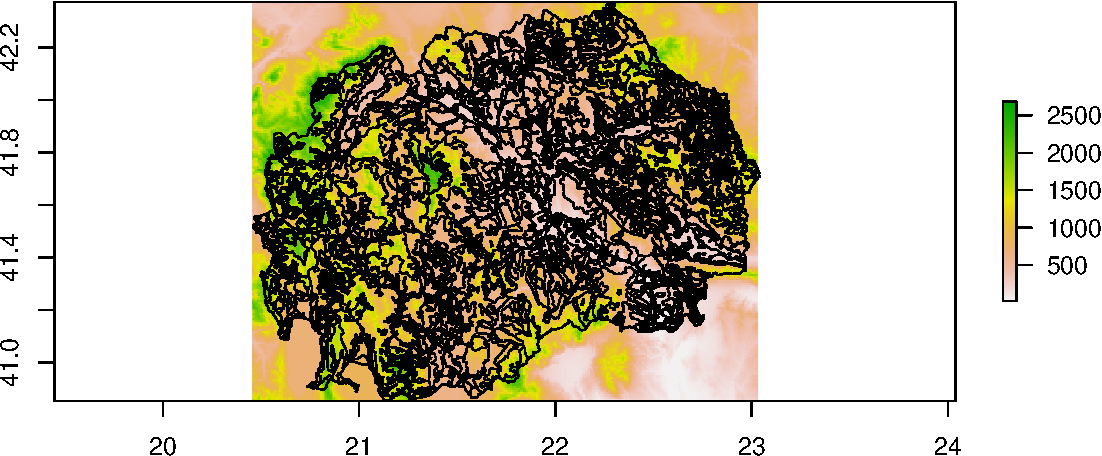
\includegraphics{SOCMapping_files/figure-latex/unnamed-chunk-17-1.pdf}

\hypertarget{land-cover-and-land-use}{%
\section{Land Cover and Land use}\label{land-cover-and-land-use}}

Besides soil, geology, and climate, land use and/or land cover data are
unarguably vital data for any statistical effort to map soil properties.
There are many of various sources of data on the land cover including
global and continental products, such as GlobCover, GeoCover,
Globeland30, CORINE Land Cover.

\begin{Shaded}
\begin{Highlighting}[]
\NormalTok{landcover <-}\StringTok{ }\KeywordTok{raster}\NormalTok{(}\StringTok{"covs/LCEE10.tif"}\NormalTok{)}

\CommentTok{# Land cover is a categorical covariate, this has to be made }
\CommentTok{# explicit using function as.factor()}
\NormalTok{landcover <-}\StringTok{ }\KeywordTok{as.factor}\NormalTok{(landcover)}
\end{Highlighting}
\end{Shaded}

\hypertarget{globcover-global}{%
\subsection{GlobCover (Global)}\label{globcover-global}}

GlobCover is a European Space Agency (ESA) initiative which began in
2005 in partnership with JRC, EEA, FAO, UNEP, GOFC-GOLD, and IGBP. The
aim of the project was to develop a service capable of delivering global
composites and land cover maps using as input observations from the 300
m MERIS sensor onboard the ENVISAT satellite mission. ESA makes
available the land cover maps, which cover 2 periods: December 2004 -
June 2006 and January - December 2009. The classification module of the
GlobCover processing chain consists in transforming the MERIS-FR
multispectral mosaics produced by the pre-processing modules into a
meaningful global land cover map. The global land cover map has been
produced in an automatic and global way and is associated with a legend
defined and documented using the UN LCCS. The GlobCover 2009 land cover
map is delivered as one global land cover map covering the entire Earth.
Its legend, which counts 22 land cover classes, has been designed to be
consistent at the global scale and therefore, it is determined by the
level of information that is available and that makes sense at this
scale \citep{bontemps2011globcover}. The GlobCover data can be
downloaded at \url{http://due.esrin.esa.int/page_globcover.php}

\hypertarget{landsat-geocover-global}{%
\subsection{Landsat GeoCover (Global)}\label{landsat-geocover-global}}

The Landsat GeoCover collection of global imagery was merged into
mosaics by the Earth Satellite Company (now MDA Federal). The result was
a series of tiled imagery that is easier to wield than individual
scenes, especially since they cover larger areas than the originals. The
great detail in these mosaic scenes, however, makes them large in
storage size, so the Mr.Sid file format, which includes compression
operations, was chosen for output. While GeoCover itself is available in
three epochs of 1975, 1990 and 2000, only the latter two epochs were
made into mosaics. Coverage: The GeoCover Landsat mosaics are delivered
in a Universal Transverse Mercator (UTM) / World Geodetic System 1984
(WGS84) projection. The mosaics extend north-south over 5 degrees of
latitude and span east-west for the full width of the UTM zone. For
mosaics below 60 degrees north latitude, the width of the mosaic is the
standard UTM zone width of 6 degrees of longitude. For mosaics above 60
degrees of latitude, the UTM zone is widened to 12 degrees, centered on
the standard even-numbered UTM meridians. To insure overlap between
adjacent UTM zones, each mosaic extends for at least 50 kilometers to
the east and west, and 1 kilometer to the north and south. Pixel size:
14.25 meters (V 2000) The data is available at
\url{ftp://ftp.glcf.umd.edu/glcf/Mosaic_Landsat/} (FTP Access)

\hypertarget{globeland30-global}{%
\subsection{Globeland30 (Global)}\label{globeland30-global}}

GlobeLand30, the world's first global land cover dataset at 30 m
resolution for the years 2000 and 2010, was recently released and made
publicly available by China. The National Geomatics Center of China
under the ``Global Land Cover Mapping at Finer Resolution'' project has
recently generated a global land cover map named GlobeLand30. The
dataset covers two timestamps of 2000 and 2010, primarily acquired from
Landsat TM and ETM+ sensors, which were then coupled/checked with some
local products. The data is publicly available for non-commercial
purposes at
\url{http://www.globallandcover.com/GLC30Download/index.aspx}\\
Further reading and other global data sources:
\url{http://worldgrids.org/doku.php/wiki:land_cover_and_land_use}

\hypertarget{corine-land-cover-europe-only}{%
\subsection{CORINE Land Cover (Europe
Only)}\label{corine-land-cover-europe-only}}

The pan-European component is coordinated by the European Environment
Agency (EEA) and produces satellite image mosaics, land cover/land use
(LC/LU) information in the CORINE Land Cover data, and the
High-Resolution Layers. The CORINE Land Cover is provided for 1990,
2000, 2006 and 2012. This vector-based dataset includes 44 land cover
and land use classes. The time-series also includes a land-change layer,
highlighting changes in land cover and land-use. The high-resolution
layers (HRL) are raster-based datasets (100 m, 250 m) which provide
information about different land cover characteristics and is
complementary to land-cover mapping (e.g.~CORINE) datasets. The CORINE
Land Cover Data are available at
\url{http://www.eea.europa.eu/data-and-maps/data}

\hypertarget{climate}{%
\section{Climate}\label{climate}}

\hypertarget{worldclim-v1.4-and-v2-global}{%
\subsection{WorldClim V1.4 and V2
(Global)}\label{worldclim-v1.4-and-v2-global}}

WorldClim is a set of global climate layers (gridded climate data) with
a spatial resolution of about 1 km2 (10 minutes, 5 minutes, 2.5 minutes
are also available). These data can be used for mapping and spatial
modeling. The current version is Version 1.4. and a preview of Version 2
is available for testing at worldclim.org. The data can be downloaded as
generic grids or in ESRI Grid format.

The WorldClim data layers were generated by interpolation of average
monthly climate data from weather stations on a 30 arc-second resolution
grid. In V1.4, variables included are monthly total precipitation, and
monthly mean, minimum and maximum temperatures, and 19 derived
bioclimatic variables. The WorldClim precipitation data were obtained
from a network of 1,473 stations, mean temperature from 24,542 stations,
and minimum and maximum temperatures from 14,835 stations
\citep{hijmans2005very}.

The Bioclimatic parameters are: annual mean temperature, mean diurnal
range, iso-thermality, temperature seasonality, max temperature of
warmest month, minimum temperature of coldest month, temperature annual
range , mean temperature of wettest quarter, mean temperature of driest
quarter, mean temperature of warmest quarter, mean temperature of
coldest quarter, annual precipitation, precipitation of wettest month,
precipitation of driest month, precipitation seasonality (coefficient of
variation), precipitation of wettest quarter, precipitation of driest
quarter, precipitation of warmest quarter, precipitation of coldest
quarter.

WorldClim Climate Data are available at: www.worldclim.org (WorldClim
1.4 (current conditions) by www.worldclim.org; \citet{hijmans2005very}.
Is licensed under a Creative Commons Attribution-ShareAlike 4.0
International License).

\begin{Shaded}
\begin{Highlighting}[]
\CommentTok{# load the climate covariates from the raster tif files}
\NormalTok{files <-}\StringTok{ }\KeywordTok{list.files}\NormalTok{(}\DataTypeTok{path =} \StringTok{"covs/"}\NormalTok{, }\DataTypeTok{pattern =} \StringTok{"CHE3.tif"}\NormalTok{, }
                    \DataTypeTok{full.names =} \OtherTok{TRUE}\NormalTok{)}

\CommentTok{# stack all the files in one RasterStack}
\NormalTok{climate <-}\StringTok{ }\KeywordTok{stack}\NormalTok{(files)}
\end{Highlighting}
\end{Shaded}

\begin{Shaded}
\begin{Highlighting}[]
\CommentTok{# plot the first 2 layers}
\KeywordTok{plot}\NormalTok{(climate[[}\DecValTok{1}\OperatorTok{:}\DecValTok{2}\NormalTok{]])}
\end{Highlighting}
\end{Shaded}

\begin{figure}
\centering
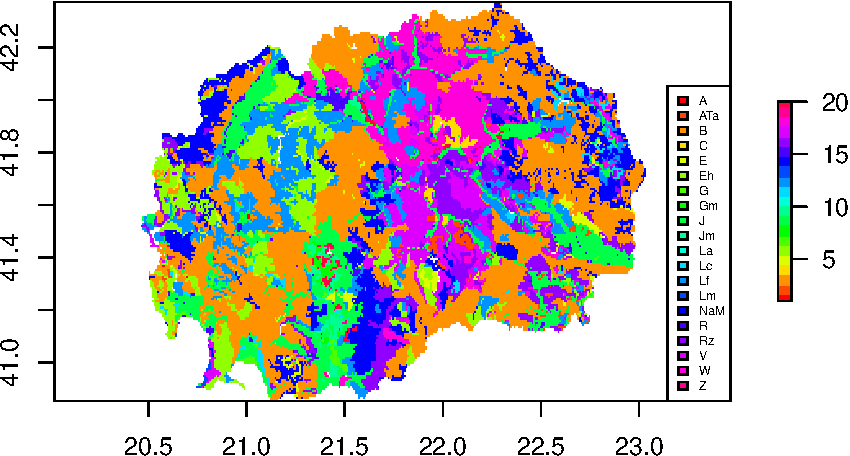
\includegraphics{SOCMapping_files/figure-latex/unnamed-chunk-20-1.pdf}
\caption{\label{fig:unnamed-chunk-20}Two layers included in the climate
covariates}
\end{figure}

\hypertarget{gridded-agro-meteorological-data-in-europe-europe}{%
\subsection{Gridded Agro-Meteorological Data in Europe
(Europe)}\label{gridded-agro-meteorological-data-in-europe-europe}}

CGMS database contains meteorological parameters from weather stations
interpolated on a 25×25 km grid. Meteorological data are available on a
daily basis from 1975 to the last calendar year completed, covering the
EU Member States, neighboring European countries.

The following parameters are available at 1-day time resolution:

\begin{itemize}
\tightlist
\item
  maximum air temperature (°C)
\item
  minimum air temperature (°C)
\item
  mean air temperature (°C)
\item
  mean daily wind speed at 10m (m/s)
\item
  mean daily vapor pressure (hPa)
\item
  sum of precipitation (mm/day)
\item
  potential evaporation from a free water surface (mm/day)
\item
  potential evapotranspiration from a crop canopy (mm/day)
\item
  potential evaporation from a moist bare soil surface (mm/day)
\item
  total global radiation (KJ/m2/day)
\item
  Snow Depth
\end{itemize}

Data Access:
\url{http://agri4cast.jrc.ec.europa.eu/DataPortal/Index.aspx}

\hypertarget{GSOCDataRepo}{%
\section{GSOCMap - Data Repository (ISRIC, 2017)}\label{GSOCDataRepo}}

ISRIC World Soil Information has established a data repository which
contains raster layers of various biophysical earth surface properties
for each territory in the world. These layers can be used as covariates
in a digital soil mapping exercise.

\hypertarget{covariates-and-empty-mask}{%
\subsection{Covariates and Empty Mask}\label{covariates-and-empty-mask}}

The territories and their boundaries are obtained from the Global
Administrative Unit Layers (GAUL)dataset: each folder contains three
subfolders; covs: GIS layers of various biophysical earth surface
properties mask: an `empty' grid file of the territory with territory
boundary according to GAUL. This grid to be used for the final delivery.
. soilgrids: all SoilGrids250m soil class and property layers as
available through www.soilgrids.org. Layers are aggregated to 1 km.

\hypertarget{data-specifications}{%
\subsection{Data Specifications}\label{data-specifications}}

File format: GeoTiff Coordinate system: WGS84, latitude-longitude in
decimal degrees Spatial resolution: 1km

\hypertarget{data-access}{%
\subsection{Data Access}\label{data-access}}

\url{ftp://gsp.isric2.org/} (username: gsp, password: gspisric) or
\url{ftp://85.214.253.67/} (username: gsp, password: gspisric)

LICENCE and ACKNOWLEDGEMENT \emph{The GIS layers can be freely used
under the condition that proper credit should be given to the original
data source in each publication or product derived from these layers.
Licences, data sources, data citations are indicated the data
description table.}

\hypertarget{extending-the-soil-property-table-for-spatial-statistics}{%
\section{Extending the Soil Property Table for Spatial
Statistics}\label{extending-the-soil-property-table-for-spatial-statistics}}

The upscaling procedures (see chapter \ref{mappingMethods}) depend on
the rationale that the accumulation of local soil carbon stocks (and
also other properties) depend on parameters for which spatial data are
available, such as climate, soil type, parent material, slope,
management. This information (Covariates) must be collected first.
Details are provided above. The properties contained in the covariates
can be extracted to each georeferenced sample site and added to the soil
property table (Table 3.1). This table is used for training and
validation of the statistical model for predicting the SOC stocks which
subsequently can be applied to the full spatial extent.

\hypertarget{preparation-of-a-soil-property-table-for-spatial-statistics}{%
\section{Preparation of a Soil Property Table for Spatial
Statistics}\label{preparation-of-a-soil-property-table-for-spatial-statistics}}

The upscaling procedures (see chapter \ref{mappingMethods}) depend on
the rationale, that the accumulation of local soil carbon concentrations
and stocks (and also other properties) depends on influential parameters
for which spatial data are available, such as climate, soil type, parent
material, slope, management. Any parameter in the table of local soil
properties, for which a spatial layer is available, may be included in
the final table. Other covariates will be added in section 3. An example
is the clay content, which may be derived from a soil type or parent
rock map.

\begin{quote}
In case this table is prepared for different depths, 0-10 cm, 10-30 cm,
and if the host institution intends to develop different spatial models
for different depths (e.g.~separate spatial prediction model for litter
and mineral soil 0-30), then the separate grids have to be added.
\end{quote}

\hypertarget{overlay-soil-covariates}{%
\section{Technical Steps - Overlay Covariates and Soil Points
Data}\label{overlay-soil-covariates}}

\hypertarget{load-soil-sample-data-and-covariates}{%
\subsection{Load soil sample data and
covariates}\label{load-soil-sample-data-and-covariates}}

\begin{Shaded}
\begin{Highlighting}[]
\CommentTok{# Load the processed data. This table was prepared in the previous }
\CommentTok{# chapter.}
\NormalTok{dat <-}\StringTok{ }\KeywordTok{read.csv}\NormalTok{(}\StringTok{"data/dat_train.csv"}\NormalTok{)}

\CommentTok{# read covariates from tif raster files}
\NormalTok{files <-}\StringTok{ }\KeywordTok{list.files}\NormalTok{(}\DataTypeTok{path =} \StringTok{"covs"}\NormalTok{, }\DataTypeTok{pattern =} \StringTok{"tif$"}\NormalTok{, }
                    \DataTypeTok{full.names =} \OtherTok{TRUE}\NormalTok{)}

\NormalTok{covs <-}\StringTok{ }\KeywordTok{stack}\NormalTok{(files)}
\end{Highlighting}
\end{Shaded}

\hypertarget{combine-the-covariates-provided-with-the-raster-version-of-the-soil-map}{%
\subsection{Combine the covariates provided with the raster version of
the soil
map}\label{combine-the-covariates-provided-with-the-raster-version-of-the-soil-map}}

\begin{Shaded}
\begin{Highlighting}[]
\CommentTok{# soilmap.r is the rasterization of the soil map and was obtained}
\CommentTok{# in a previous step}
\NormalTok{covs <-}\StringTok{ }\KeywordTok{stack}\NormalTok{(covs, soilmap.r)}

\CommentTok{# correct the name for layer 14}
\KeywordTok{names}\NormalTok{(covs)[}\DecValTok{14}\NormalTok{] <-}\StringTok{ "soilmap"}
\end{Highlighting}
\end{Shaded}

Finally, we will mask the covariates with a mask developed using the
country limits. Next, we will export all the covariates as 1 file. This
will allow us to load this file in the following chapters of this book.

\begin{Shaded}
\begin{Highlighting}[]
\CommentTok{#mask the covariates with the country mask from the data repository}
\NormalTok{mask <-}\StringTok{ }\KeywordTok{raster}\NormalTok{(}\StringTok{"data/mask.tif"}\NormalTok{)}
\NormalTok{covs <-}\StringTok{ }\KeywordTok{mask}\NormalTok{(}\DataTypeTok{x =}\NormalTok{ covs, }\DataTypeTok{mask =}\NormalTok{ mask)}

\CommentTok{# export all the covariates }
\KeywordTok{save}\NormalTok{(covs, }\DataTypeTok{file =} \StringTok{"covariates.RData"}\NormalTok{)}

\KeywordTok{plot}\NormalTok{(covs)}
\end{Highlighting}
\end{Shaded}

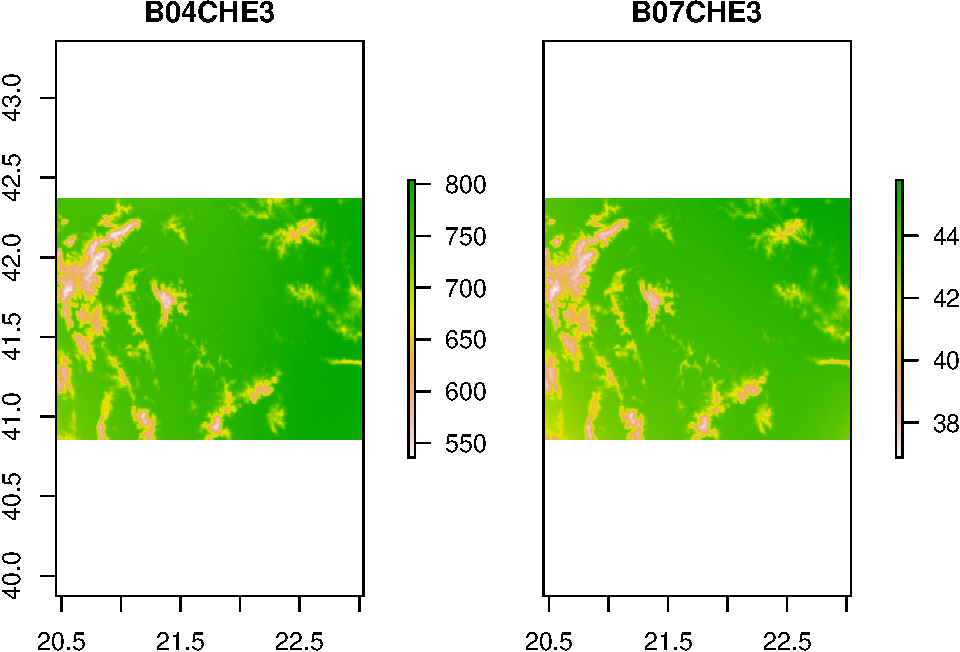
\includegraphics{SOCMapping_files/figure-latex/unnamed-chunk-23-1.pdf}

\hypertarget{overlay-covariates-and-spatial-data}{%
\subsection{Overlay Covariates and Spatial
Data}\label{overlay-covariates-and-spatial-data}}

In order to carry out digital soil mapping in terms of examining the
statistical significance of environmental predictors for explaining the
spatial variation of SOC, we should link both sets of data together and
extract the values of the covariates at the locations of the soil point
data. Note that the stacking of rasters can only be possible if they are
in the same resolution and extent. If they are not, \textbf{raster}
package resample and \texttt{projectRaster()} functions are for
harmonizing all your different raster layers. With the stacked rasters
(Covstack), we can now perform the intersection and extraction.

\begin{Shaded}
\begin{Highlighting}[]
\CommentTok{#upgrade points data frame to SpatialPointsDataFrame}
\KeywordTok{coordinates}\NormalTok{(dat) <-}\StringTok{ }\ErrorTok{~}\StringTok{ }\NormalTok{X }\OperatorTok{+}\StringTok{ }\NormalTok{Y}

\CommentTok{# extract values from covariates to the soil points}
\NormalTok{dat <-}\StringTok{ }\KeywordTok{extract}\NormalTok{(}\DataTypeTok{x =}\NormalTok{ covs, }\DataTypeTok{y =}\NormalTok{ dat, }\DataTypeTok{sp =} \OtherTok{TRUE}\NormalTok{)}

\CommentTok{# LCEE10 and soilmap are categorical variables}
\NormalTok{dat}\OperatorTok{@}\NormalTok{data}\OperatorTok{$}\NormalTok{LCEE10 <-}\StringTok{ }\KeywordTok{as.factor}\NormalTok{(dat}\OperatorTok{@}\NormalTok{data}\OperatorTok{$}\NormalTok{LCEE10)}
\NormalTok{dat}\OperatorTok{@}\NormalTok{data}\OperatorTok{$}\NormalTok{soilmap <-}\StringTok{ }\KeywordTok{as.factor}\NormalTok{(dat}\OperatorTok{@}\NormalTok{data}\OperatorTok{$}\NormalTok{soilmap)}

\KeywordTok{levels}\NormalTok{(soilmap) <-}\StringTok{ }\NormalTok{Symbol.levels}

\KeywordTok{summary}\NormalTok{(dat}\OperatorTok{@}\NormalTok{data)}
\end{Highlighting}
\end{Shaded}

\begin{verbatim}
##        id            SOC              BLD         
##  P0003  :   1   Min.   : 0.080   Min.   :0.05353  
##  P0007  :   1   1st Qu.: 1.772   1st Qu.:1.27881  
##  P0008  :   1   Median : 2.620   Median :1.39605  
##  P0009  :   1   Mean   : 3.579   Mean   :1.37990  
##  P0010  :   1   3rd Qu.: 4.090   3rd Qu.:1.47619  
##  P0011  :   1   Max.   :86.510   Max.   :2.89888  
##  (Other):2910                                     
##      CRFVOL             OCSKGM           meaERROR    
##  Min.   : 0.00000   Min.   :0.03524   Min.   :0.172  
##  1st Qu.: 0.01195   1st Qu.:0.70410   1st Qu.:3.160  
##  Median : 5.00000   Median :0.99674   Median :3.830  
##  Mean   :10.91665   Mean   :1.15062   Mean   :3.717  
##  3rd Qu.:17.19974   3rd Qu.:1.40756   3rd Qu.:4.260  
##  Max.   :93.95013   Max.   :7.43023   Max.   :8.620  
##                                                      
##    OCSKGMlog            B04CHE3         B07CHE3     
##  Min.   :-3.345652   Min.   :547.2   Min.   :37.60  
##  1st Qu.:-0.350842   1st Qu.:759.8   1st Qu.:43.74  
##  Median :-0.003263   Median :763.9   Median :44.06  
##  Mean   :-0.008980   Mean   :759.3   Mean   :43.88  
##  3rd Qu.: 0.341860   3rd Qu.:774.8   3rd Qu.:44.54  
##  Max.   : 2.005557   Max.   :802.9   Max.   :45.39  
##                                                     
##     B13CHE3          B14CHE3         DEMENV5        LCEE10    
##  Min.   : 45.71   Min.   :22.26   Min.   :  45.0   1   :1967  
##  1st Qu.: 60.01   1st Qu.:27.70   1st Qu.: 395.5   2   : 698  
##  Median : 71.19   Median :30.11   Median : 594.0   3   :  94  
##  Mean   : 74.26   Mean   :32.31   Mean   : 655.8   4   : 156  
##  3rd Qu.: 78.79   3rd Qu.:35.61   3rd Qu.: 814.2   NA's:   1  
##  Max.   :167.31   Max.   :60.32   Max.   :2375.0              
##                                                               
##     PRSCHE3          SLPMRG5          TMDMOD3     
##  Min.   : 430.4   Min.   : 0.000   Min.   :280.0  
##  1st Qu.: 529.9   1st Qu.: 0.000   1st Qu.:291.0  
##  Median : 565.4   Median : 4.000   Median :293.0  
##  Mean   : 604.6   Mean   : 8.553   Mean   :292.3  
##  3rd Qu.: 651.3   3rd Qu.:13.000   3rd Qu.:294.0  
##  Max.   :1211.9   Max.   :61.000   Max.   :297.0  
##                                                   
##     TMNMOD3         TWIMRG5          VBFMRG5     
##  Min.   :270.0   Min.   : 56.00   Min.   :  0.0  
##  1st Qu.:279.0   1st Qu.: 79.00   1st Qu.:  0.0  
##  Median :280.0   Median : 94.00   Median : 70.5  
##  Mean   :279.7   Mean   : 91.12   Mean   :173.6  
##  3rd Qu.:281.0   3rd Qu.:102.00   3rd Qu.:390.0  
##  Max.   :284.0   Max.   :139.00   Max.   :498.0  
##                                                  
##     VDPMRG5         soilmap   
##  Min.   :-5869   9      :857  
##  1st Qu.: 3571   3      :425  
##  Median : 5702   12     :217  
##  Mean   : 5370   10     :211  
##  3rd Qu.: 7024   14     :205  
##  Max.   :14104   (Other):982  
##                  NA's   : 19
\end{verbatim}

After the extraction, it's useful to check if there are missing values
(\texttt{NAs}) both in the target variable and covariates. In these
cases, these data should be excluded. A quick way to assess if there are
missing or NA values in the data is to use the \texttt{complete.cases()}
function.

After removing NAs, now there do not appear to be any missing data as
indicated by the \texttt{integer(0)} output above. It means we have zero
rows with missing information.

The last step involves exporting a table our regression matrix including
the soil data and the values of the environmental covariates in the
position of the point samples.

The summary of the \texttt{dat\ data.frame} shows 1 points with NA
values for most of the covariates. And 22 points with NA values in the
soilmap layer. The regression matrix should not contain NA values. There
are two options to proceed:

\begin{itemize}
\item
  \textbf{Option 1}: In some cases, this NA values are from points with
  bad position data. Therefore, the points area outside the study area.
  In this case, the solution is to correct the coordinates or eliminate
  the points. This is the case for the two points with NA values for
  most of the covariates.
\item
  \textbf{Option 2}: Another case is when a covariate is incomplete and
  does not cover all the area. This could produce many NA values. There
  are two different solutions, either to eliminate the covariate or to
  eliminate the point data. This is the case for the soilmap layer and
  the 30 points.
\end{itemize}

\hypertarget{convert-result-to-data.frame-and-save-as-a-csv-table}{%
\subsection{Convert result to data.frame and save as a csv
table}\label{convert-result-to-data.frame-and-save-as-a-csv-table}}

\begin{Shaded}
\begin{Highlighting}[]
\NormalTok{dat <-}\StringTok{ }\KeywordTok{as.data.frame}\NormalTok{(dat)}

\CommentTok{# The points with NA values has to be removed }
\NormalTok{dat <-}\StringTok{ }\NormalTok{dat[}\KeywordTok{complete.cases}\NormalTok{(dat),]}

\CommentTok{# export as a csv table}
\KeywordTok{write.csv}\NormalTok{(dat, }\StringTok{"data/MKD_RegMatrix.csv"}\NormalTok{, }\DataTypeTok{row.names =} \OtherTok{FALSE}\NormalTok{)}
\end{Highlighting}
\end{Shaded}

\hypertarget{mappingMethods}{%
\chapter{Mapping Methods}\label{mappingMethods}}

\emph{R Baritz, M Guevara, VL Mulder, GF Olmedo, C Thine, RR Vargas, Y
Yigini}

In this chapter, we want to introduce 5 different approaches for
obtaining the SOC map for FYROM. The first two methods presented are
classified as conventional upscaling. The first one is class-matching.
In this approach, we derive average SOC stocks per class: soil type for
which a national map exists, or combination with other spatial
covariates (e.g.~land use category, climate type, biome, etc.). This
approach is used in the absence of spatial coordinates of the source
data. The second one is geo-matching, were upscaling is based on
averaged SOC values per mapping unit. Then, we present 3 methods from
digital soil mapping. Regression-Kriging is a hybrid model with both, a
deterministic and a stochastic component \citep{hengl2007regression}.
Next method is called random forest. This one is an ensemble of
regression trees based on bagging. This machine learning algorithm uses
a different combination of prediction factors to train multiple
regression trees \citep{Breiman1996}. The last method is called Support
Vector Machines (SVM). This method applies a simple linear method to the
data but in a high-dimensional feature space non-linearly related to the
input space \citep{Karatzoglou2006}. We present this diversity of
methods because there is no best mapping method for digital soil
mapping, and testing and selection has to be done for every data
scenario \citep{soil-2017-40}.

\hypertarget{conventional-upscaling-using-soil-maps}{%
\section{Conventional Upscaling Using Soil
Maps}\label{conventional-upscaling-using-soil-maps}}

\emph{R Baritz, VL Mulder}

\hypertarget{overview}{%
\subsection{Overview}\label{overview}}

The two conventional upscaling methods, in the context of SOC mapping,
are described by \cite{lettens2004soil}. Details about weighted
averaging can be found in \cite{hiederer2013mapping}. Different
conventional upscaling approaches were applied in many countries (Baritz
et al.~1999 (Germany), \cite{krasilnikov2013soils} (Mexico),
\cite{greve2007generating} (Denmark), Koelli et al.~2009 (Estonia),
\cite{arrouays2001carbon} (France), \cite{bhatti2002estimates}
(Canada)). Because the structure of soil map databases differs between
countries (definition of the soil mapping unit, stratification, soil
associations, dominating and co-dominating soils, typical and estimate
soil properties for different depths), it is difficult to define a
generic methodology for the use of these maps for mapping soil property
information.

However, the essential principle which is commonly used is to combine
soil property data from local observations with soil maps via class- and
geomatching.

\textbf{Diversity of national soil legacy data sets} in order to develop
a representative and large national soil database, very often, data from
different sources (e.g.~soil surveys or projects in different parts of
the country at different times) are combined. The following case of
Belgium demonstrates how available legacy databases could be combined.
Three different sources are used to compile an overview of national SOC
stocks:

\textbf{Data source 1}: soil profile database with 13,000 points of
genetic horizons; for each site, there is information about the soil
series, map coordinates, and land use class; for each horizon, there is
information about depth and thickness, textural fractions and class,
volume percentage of rock fragments; analytically, there is the organic
carbon content and inorganic carbon content.

\textbf{Data source 2}: forest soil data base which includes ectorganic
horizons. According to their national definition, the term
``ectorganic'' designates the surface horizons with an organic matter
content of at least \(30\%\), thus, it includes both the litter layer
and the organic soil layers. For the calculation of SOC stocks for the
ectorganic layer, no fixed-depth was used, instead, the measured
thickness of the organic layers and litter layers was applied.

\textbf{Data source 3}: 15,000 soil surface samples were used (upper 20
cm of mineral soil); carbon measurements are available per depth class.

From all data sources, SOC stocks for peat soils were calculated
separately.

\hypertarget{technical-steps-class-matching}{%
\subsection{Technical Steps:
Class-matching}\label{technical-steps-class-matching}}

\hypertarget{data-preparation}{%
\subsubsection{Data Preparation}\label{data-preparation}}

\begin{itemize}
\tightlist
\item
  Separate the database for forests, peat, and other land uses If only
  horizons are provided: derive or estimate average depth of horizons
  per soil type; add upper and lower depth.
\item
  Check completeness of parameters per depth using the solum depth to
  code empty cells
\item
  Correction of organic carbon in case total carbon was determined
  (total carbon minus inorganic carbon concentration)
\item
  Correction of Walkley and Black method for incomplete oxidation (1.32)
\item
  If BD measured is lacking, select proper pedotransfer functions (PTF)
  and estimate BD. There are many PTF. At best, publications about the
  choice of the best suited PTF for specific physio-geographic
  conditions are available.
\item
  If the stone content is missing, investigate using other data sources
  or literature, to which a correction for stones should be applied
\item
  if possible, derive the standard average stone content for different
  soils/horizons/depths, or used published soil profiles, as a simple
  correction factor.
\item
  Calculate SOC stocks for all mineral and peat soils over 0-30 cm, and
  optionally for forest organic layers and, peat \textgreater{}30
  \textless{}100 cm.
\end{itemize}

\hypertarget{preparatory-gis-operations}{%
\subsubsection{Preparatory GIS
Operations}\label{preparatory-gis-operations}}

\begin{itemize}
\tightlist
\item
  Prepare Covariates
\item
  Identify properties of covariates for each point observation using
  geo-matching
\item
  Mapping using geo-matching of all points: Extract the covariate
  information to all georeferenced sample sites. The SOC values from all
  points within the unit are then averaged. It is assumed that the
  points represent the real variability of soil types within the units
\end{itemize}

\hypertarget{mapping}{%
\subsubsection{Mapping}\label{mapping}}

\begin{itemize}
\tightlist
\item
  Mapping using class-matching of points in agreement with classes
\end{itemize}

Through \emph{class-matching}, only those points or profiles are
attributed to a soil or landscape unit if both the soil and the land use
class are the same. Class-matching thus can be performed regardless of
the profile location. Before averaging, a weighing factor can be
introduced according to the area proportions of dominant, co-dominant
and associated soils. Each profile needs to be matched to its soil
type/landscape type, and the SOC value averaged. 1. Determine a soil or
landscape unit (e.g.~national soil legend stratified by climate area and
mainland cover type (forest, grassland, cropland) 2. Calculate average
SOC stocks from all soils which match the soil/landscape unit 3. Present
the Soil/landscape map with SOC stocks, do not classify SOC stocks into
groups (e.g. \textless{} 50, 50-100, \textgreater{} 100).

Note: Pre-classified SOC maps cannot be integrated into a global GSOCmap
legend.

\begin{itemize}
\tightlist
\item
  Mapping using geo-matching
\end{itemize}

Because of its importance, geo-matching is described in more detail.

\hypertarget{technical-steps-geo-matching}{%
\subsection{Technical Steps:
Geo-Matching}\label{technical-steps-geo-matching}}

It is important to first prepare the working environment pre-processed
all input data. The following section presents different Geo-matching
procedures;

\begin{enumerate}
\def\labelenumi{\arabic{enumi}.}
\tightlist
\item
  Setting up software and working environment
\item
  Geo-matching SOC with WRB Soil map (step-by-step, using the Soil Map
  of FYROM and the demonstration data presented above)
\item
  Geo-matching SOC with other environmental variables: Land use
\item
  Finally, the development of Landscape Units (Lettens et al.~2004) is
  outlined.
\end{enumerate}

This example was developed for QGIS and focusses on SOC mapping using
vector data. QGIS 2.18 with GRASS 7.05 will be used. For more
information, see also:

\begin{itemize}
\tightlist
\item
  \url{https://gis.stackexchange.com}
\item
  \url{http://www.qgis.org/}
\item
  \url{http://www.qgisforum.org/}
\end{itemize}

\hypertarget{setting-up-a-qgis-project}{%
\subsubsection{Setting Up a QGIS
Project}\label{setting-up-a-qgis-project}}

\begin{enumerate}
\def\labelenumi{\arabic{enumi}.}
\tightlist
\item
  Install QGIS and supporting software; download the software at
  \url{http://www.qgis.org/en/site/forusers/download.html} (select
  correct version for Windows, Mac or Linux, 32 or 64 bit).
\item
  Create a work folder,
  e.g.~D:\textbackslash{}GSOC\textbackslash{}practical\_matching. Copy
  the folder with the FYROM demonstration data into this folder.
\item
  Start `QGIS desktop with GRASS'. Fig. \ref{fig:qgis} shows the start
  screen of QGIS desktop. In the upper left panel, there is the browser
  panel, which lists the geodata used for this example. In the bottom
  left, the layer information is given for the layers displayed on the
  right.
\end{enumerate}

\begin{figure}

{\centering 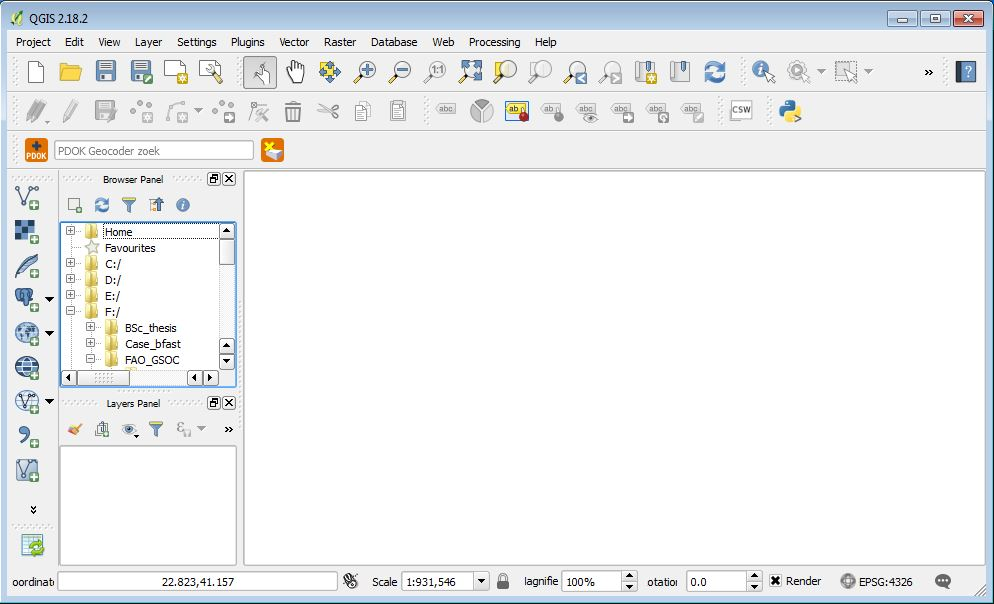
\includegraphics[width=0.8\linewidth]{images/Conv_upscaling1} 

}

\caption{QGIS Desktop with the browser panel on the upper left, the layer information on the bottom left and the display of your layers on the right}\label{fig:qgis}
\end{figure}

\begin{enumerate}
\def\labelenumi{\arabic{enumi}.}
\setcounter{enumi}{3}
\tightlist
\item
  Load the FYROM soil map. Right-click the file in the Browser panel and
  add the map to your project.
\item
  Display the soil classes. Right-click on the file in the Layers Panel,
  properties. Go to Style and change from `Single symbol' to
  `Categorized' (Fig. \ref{fig:layerprop}). Select the column `WRB' and
  press the icon `Classify' and change the colors if you want. Next,
  apply the change and finish by clicking the OK-button.
\end{enumerate}

\begin{figure}

{\centering 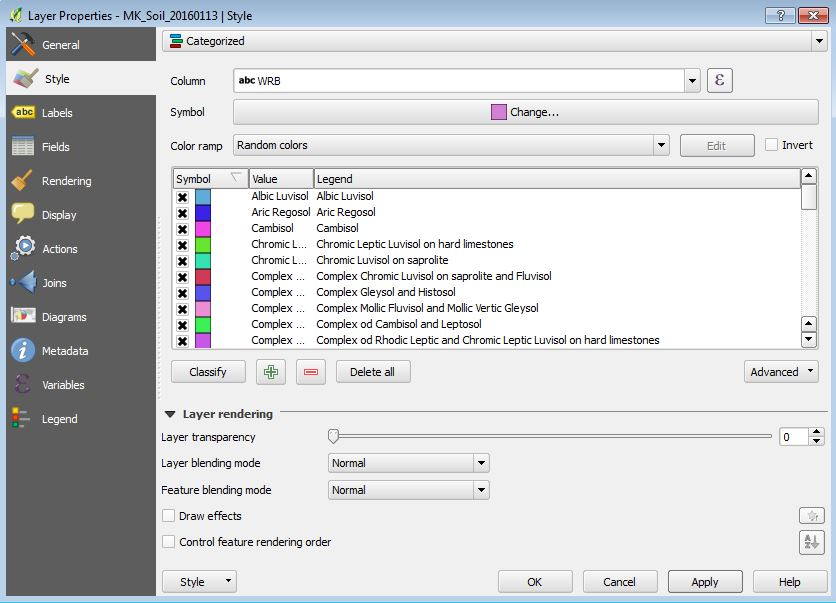
\includegraphics[width=0.8\linewidth]{images/Conv_upscaling2} 

}

\caption{Changing layer properties for the FYROM Soil Map}\label{fig:layerprop}
\end{figure}

\begin{enumerate}
\def\labelenumi{\arabic{enumi}.}
\setcounter{enumi}{5}
\tightlist
\item
  Ensure the correct projection for this project. Go to: Project
  -\textgreater{} Project properties -\textgreater{} CRS In this case,
  you automatically use the local projection for FYROM. The EPSG code is
  3909 which corresponds to MGI 1901/ Balkans zone 7 (Fig.
  \ref{fig:qgisepsg}).
\end{enumerate}

\begin{figure}

{\centering 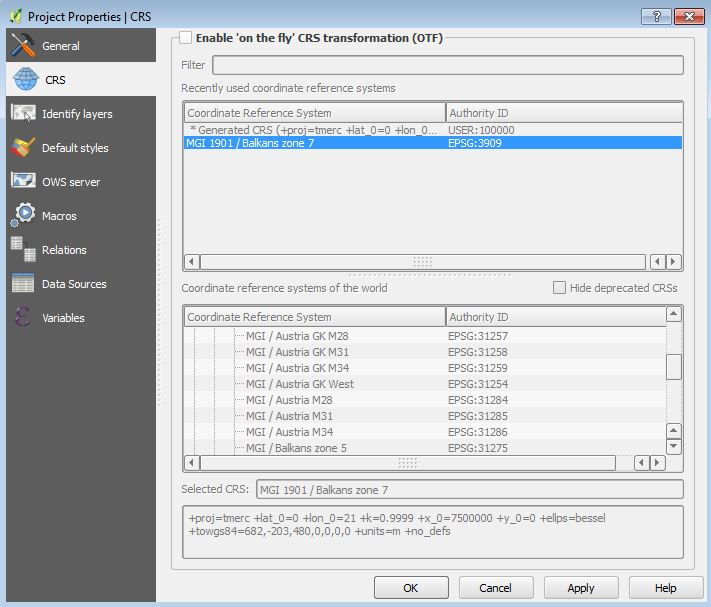
\includegraphics[width=0.8\linewidth]{images/Conv_upscaling3} 

}

\caption{Project properties and projection settings}\label{fig:qgisepsg}
\end{figure}

\begin{enumerate}
\def\labelenumi{\arabic{enumi}.}
\setcounter{enumi}{6}
\tightlist
\item
  Save the project in the created folder Load and display the
  pre-processed SOC point data. If a shapefile already exists, this is
  done the same way as described in Step 4. If you have the data as a
  text file, you need to create a vector layer out of that file. Go to
  Layer -\textgreater{} Add Layer -\textgreater{} Add Delimited Text
  layer. Select the correct file and proper CRS projection. The layer
  should be added to your Layers Panel and displayed on top of the Soil
  Map.
\end{enumerate}

\hypertarget{geo-matching-soc-with-wrb-soil-map}{%
\subsubsection{Geo-Matching SOC with WRB Soil
Map}\label{geo-matching-soc-with-wrb-soil-map}}

In this section you will make a SOC map, based on the FYROM Soil Map and
the SOC values at the sampled points, following 3 steps: 1) Extract the
soil map information for the point data, 2) obtain the mean and standard
deviation of the SOC stocks per soil class, based on the point data and
3) assign these values to the corresponding soil map units. The steps
are detailed below:

\begin{enumerate}
\def\labelenumi{\arabic{enumi}.}
\tightlist
\item
  Extract the soil map information to the soil profile data by `Join
  Attributes by location'. Vector -\textgreater{} Data Management Tools
  -\textgreater{} Join Attributes by location. Here, the target vector
  layers are the soil point data, and the join vector layer is the FYROM
  Soil Map. The geometric predicate is `intersects'. Specify at the
  `joined table' to keep only matching records and save the `joined
  layer' as a new file (Fig. 8.4).
\end{enumerate}

\begin{figure}

{\centering 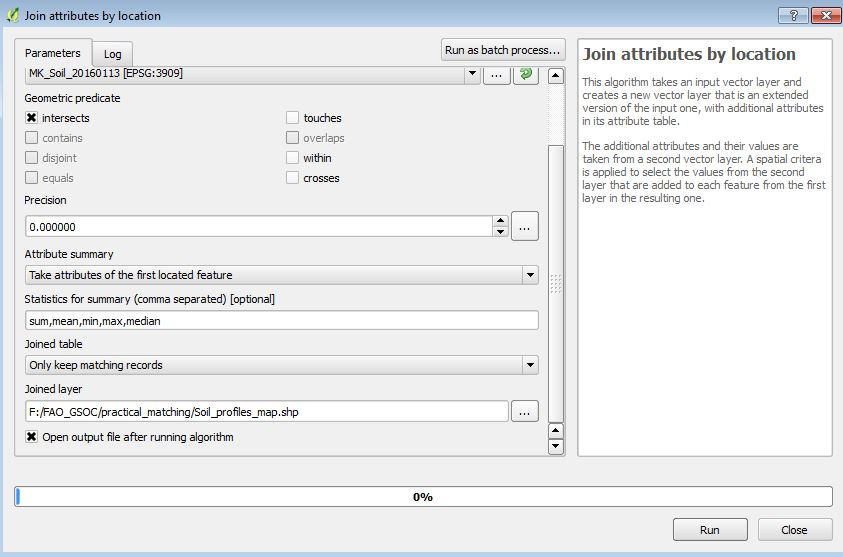
\includegraphics[width=0.8\linewidth]{images/Conv_upscaling4} 

}

\caption{Join attributes by location}\label{fig:unnamed-chunk-26}
\end{figure}

\begin{enumerate}
\def\labelenumi{\arabic{enumi}.}
\setcounter{enumi}{1}
\tightlist
\item
  Check the newly generated file, open the attribute table. The new file
  is added to the `Layers Panel' . Right-click on the file and open the
  attribute table. The information from the FYROM Soil Map is now added
  to the soil point data.
\item
  Most likely, the SOC values in the table are not numeric and thus
  statistics cannot be calculated. Check the data format, right-click on
  the file in the `Layers Panel' and check the Type name of the SOC
  field under the tab `Fields'. If they are not integer then change the
  format.
\item
  Change of the data format: Open the attribute table and start editing
  (the pencil symbol in the upper left corner of your table). Open the
  field calculator and follow these instructions (Fig. 8.5):
\end{enumerate}

\begin{enumerate}
\def\labelenumi{\alph{enumi}.}
\tightlist
\item
  Checkbox: Create a new field
\item
  Output field name: Specify the name of your field
\item
  Output field type: Decimal Number (real)
\item
  Output field length: 10, precision: 3

  \begin{enumerate}
  \def\labelenumii{\roman{enumii}.}
  \tightlist
  \item
    Expression: to\_real(`SOC'), the to\_real function can be found
    under `conversions' and the `SOC' field is found under `Fields and
    Values'
  \end{enumerate}
\end{enumerate}

\begin{figure}

{\centering 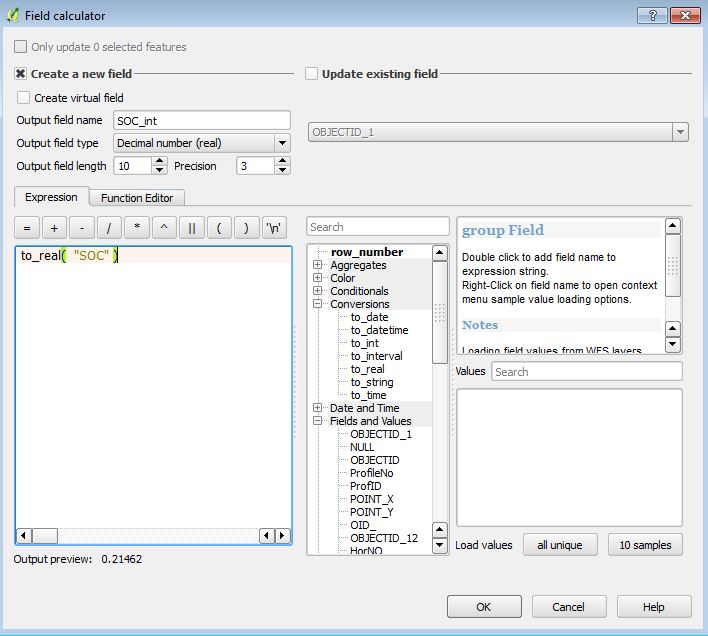
\includegraphics[width=0.8\linewidth]{images/Conv_upscaling5} 

}

\caption{Example field calculator}\label{fig:unnamed-chunk-27}
\end{figure}

\begin{enumerate}
\def\labelenumi{\arabic{enumi}.}
\setcounter{enumi}{4}
\tightlist
\item
  After calculating the field, save edits and leave the editing mode
  prior to closing the table. If changes are not saved, the added field
  will be lost.
\item
  Calculate the median SOC stock per soil type. Go to the tab
  `Vector'-\textgreater{} group stats. Select the layer from the spatial
  join you made in Step 2. Add the field `SOC' and median to the box
  with `Values' and the field `WRB' to the `Rows'. Make sure the box
  with `use only selected features' is not checked. Now calculate the
  statistics. A table will be given in the left pane (Figure 8.6). Save
  this file as .csv and repeat the same for the standard deviation.
\end{enumerate}

\begin{figure}

{\centering 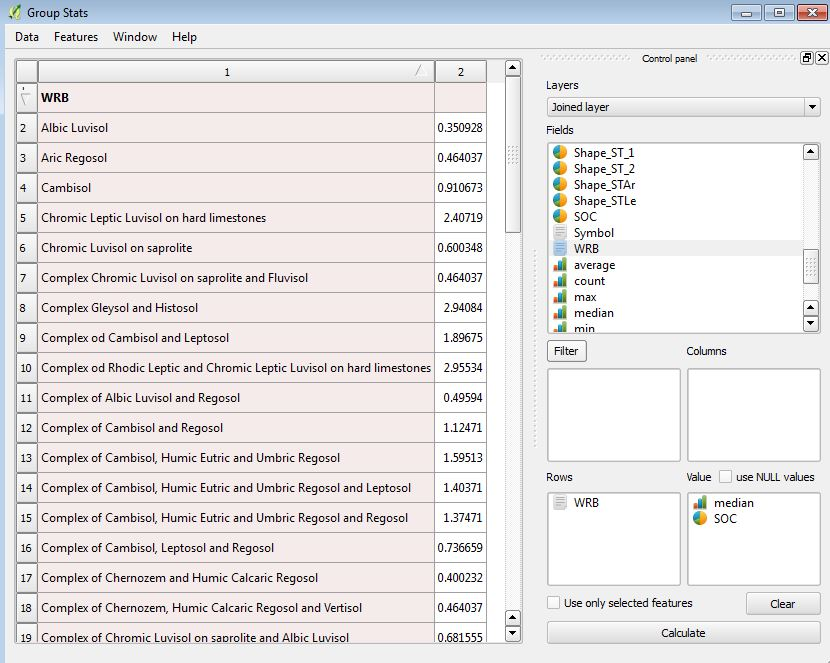
\includegraphics[width=0.8\linewidth]{images/Conv_upscaling6} 

}

\caption{Calculate group statistics}\label{fig:unnamed-chunk-28}
\end{figure}

\begin{enumerate}
\def\labelenumi{\arabic{enumi}.}
\setcounter{enumi}{6}
\tightlist
\item
  Join the mean and standard deviation of SOC to the Soil Map. First,
  add the files generated during step 6 to the Layers Panels. In the
  Layers Panel, right-click on the FYROM Soil Map. Go to Properties
  -\textgreater{} Joins and add a new join for both the median and
  standard deviation of SOC. The Join and Target Field are both `WRB'.
\item
  Display the SOC maps. Go to the layer properties of the FYROM Soil
  Map. Go to Style and change the legend to a graduated legend. In the
  column, you indicate the assigned SOC values. Probably this is not a
  integer number and so you have to convert this number again to a
  numeric values. You can do this with the box next to the box (Fig.
  8.7). Change the number of classes to e.g.~10 classes, change the mode
  of the legend and change the color scheme if you want and apply the
  settings. Now you have a map with the median SOC stocks per WRB soil
  class.
\end{enumerate}

\begin{figure}

{\centering 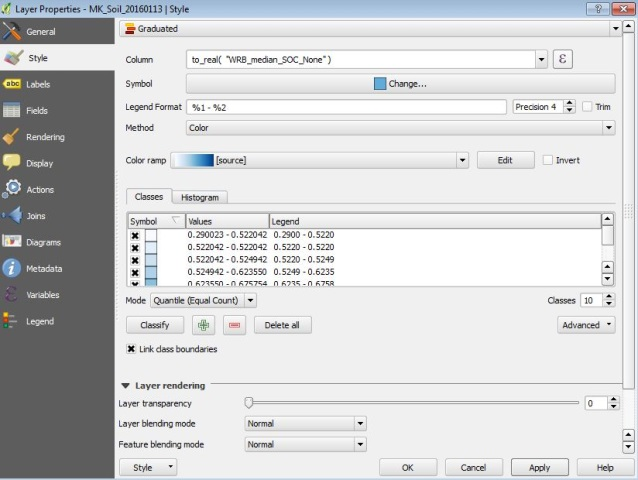
\includegraphics[width=0.8\linewidth]{images/Conv_upscaling7} 

}

\caption{Change the legend style to display the SOC values}\label{fig:unnamed-chunk-29}
\end{figure}

\begin{enumerate}
\def\labelenumi{\arabic{enumi}.}
\setcounter{enumi}{8}
\tightlist
\item
  In order to generate a proper layout, go to Project -\textgreater{}
  New Print Composer
\end{enumerate}

\begin{enumerate}
\def\labelenumi{\alph{enumi}.}
\tightlist
\item
  Add map using Layout -\textgreater{} Add Map. Define a square on the
  canvas and the selected map will be displayed.
\item
  Similarly, title, scale bar, legend and a north arrow can be added.
  Specific properties can be changed in the box `Item properties'.
\item
  When the map is finished, it can be exported as an image or pdf.
\end{enumerate}

\begin{figure}

{\centering 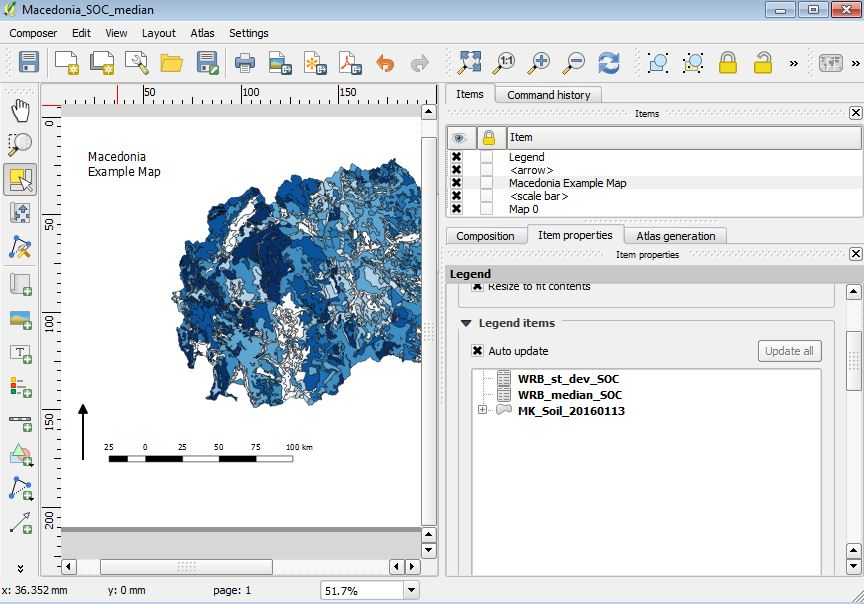
\includegraphics[width=0.8\linewidth]{images/Conv_upscaling8} 

}

\caption{Example of the Map composer}\label{fig:unnamed-chunk-30}
\end{figure}

\begin{enumerate}
\def\labelenumi{\arabic{enumi}.}
\setcounter{enumi}{9}
\tightlist
\item
  Repeat step 2-8 but now for the standard deviation of the SOC stocks.
\item
  Save the file as a new shapefile: Go to `Layer Panels -\textgreater{}
  Save as -\textgreater{} ESRI ShapeFile and make sure that you define
  the symbology export: Feature Symbology. Now, a shapefile is
  generated, with both the median and standard deviation SOC stock per
  soil type. Redundant fields can be removed after the new file is
  created.
\end{enumerate}

\hypertarget{geo-matching-soc-with-other-environmental-variables-land-use}{%
\subsubsection{Geo-Matching SOC with Other Environmental Variables: Land
Use}\label{geo-matching-soc-with-other-environmental-variables-land-use}}

\begin{enumerate}
\def\labelenumi{\arabic{enumi}.}
\tightlist
\item
  Start a new project and add the soil point data and FYROM Soil Map
  layers from the Browser panel
\item
  Add the Land Use raster file to the Layers Panels. This is a raster
  file with 1-kilometer resolution and projected in lat-long degrees
  (WGS84). For more information about this product see the online
  information from worldgrids:
  \url{http://worldgrids.org/doku.php/wiki:glcesa3}
\item
  Change the projection to the MGI 1901/ Balkans region7. Go to Raster
  -\textgreater{} Projections -\textgreater{} Warp and select the proper
  projection and a suitable file name, e.g.~LU\_projected\_1km. Tick the
  checkbox for the resampling method and choose Near. This is the
  nearest neighbor and most suitable for a transformation of categorical
  data, such as land use (Fig. 8.9).
\end{enumerate}

\begin{figure}

{\centering 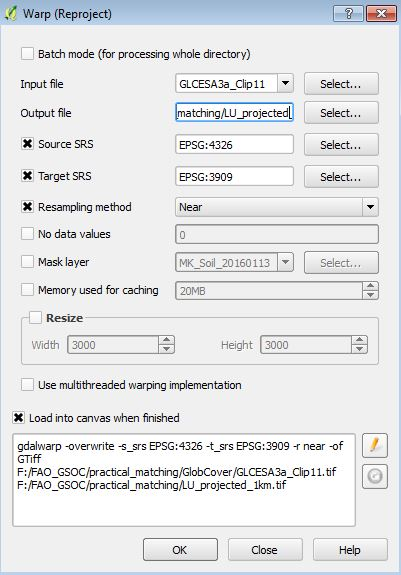
\includegraphics[width=0.8\linewidth]{images/Conv_upscaling9} 

}

\caption{Change the projection of a raster file}\label{fig:unnamed-chunk-31}
\end{figure}

\begin{enumerate}
\def\labelenumi{\arabic{enumi}.}
\setcounter{enumi}{3}
\tightlist
\item
  In order to geomatch the soil point data with Land Use, the raster
  file needs to be converted into a vector file. Go to Raster
  -\textgreater{} Conversions -\textgreater{} Polygonize. Set a proper
  output filename, e.g.~LU\_polygon\_1km, and check the tickbox for
  Fieldname.
\item
  Change the legend style into categories (Step 1-5): Now, the steps
  from the previous section need to be repeated, using the land use
  polygon map instead of using the FYROM Soil Map.
\item
  Join attributes by location using the soil point data and the polygon
  land use map.
\item
  Calculate the median and standard deviation of SOC by using the Group
  Statistics for SOC and the Land Use classes and save the files as
  .csv.
\item
  Add the generated .csv files to the Layers Panel.
\item
  Join the files with the LU polygon map, generated at step 3-4.
\item
  Change the classes in the legend and inspect the histogram with the
  median SOC values. Try to find a proper definition of the class
  boundaries (Step 2-8).
\end{enumerate}

\hypertarget{joining-landscape-units-and-soil-mapping-units-to-support-class--and-geo-matching-optional}{%
\subsubsection{Joining Landscape Units and Soil Mapping Units to Support
Class- and Geo-Matching
(Optional)}\label{joining-landscape-units-and-soil-mapping-units-to-support-class--and-geo-matching-optional}}

In this section, it is outlined how SOC stocks can be mapped following
the method outlined by \cite{lettens2004soil}. The general idea is that
the landscape is stratified into more or less homogenous units and
subsequently, the SOC stocks are obtained following the procedure
outlined earlier in this practical. \cite{lettens2004soil} outlines a
method to stratify the landscape into homogeneous strata with respect to
Land Use and Soil Type, as was explained earlier. In order to obtain
such strata, the Soil Map and the Land Use map need to be combined. This
can be done using various types of software, e.g.~ArcMap, GRASS, QGIS or
R. When using the GIS software, the only thing that needs to be done is
intersecting the vector files and dissolving the newly created polygon
features. Depending on the software and the quality of your shapefile
you may experience problems with the geometry of your shapefile.
Generally, ArcMap and GRASS correct the geometry when the shapefile is
loaded, while QGIS does not do this automatically. There are various
ways to correct the geometry, however, correcting the geometry falls
outside the scope of this training. Therefore, we give some hints on how
to correct your geometry prior to using the functions `Intersect' and
`Dissolve'.

\begin{enumerate}
\def\labelenumi{\arabic{enumi}.}
\tightlist
\item
  Change the LU raster map to 5-kilometer resolution: Right-click the
  Lu\_project\_1km file and select Save as. Change the resolution to
  5000 meters. Scroll down, check the Pyramids box, and change the
  resampling method to Nearest Neighbour.
\item
  Convert the raster map to a polygon map and add the file to the Layers
  Panel
\item
  Check the validity of the Soil Map and Land Use Map: Vector
  -\textgreater{} Geometry Tools -\textgreater{} Check Validity Below
  you find the instructions in case you have no problems with your
  geometry:
\item
  Intersect the Soil Map and the Land Use Map. In ArcGIS and QGIS you
  can use this function. Go to Vector -\textgreater{} Geoprocessing
  tools -\textgreater{} Intersection. (In GRASS you have to use the
  function `Overlay' from the Vector menu)
\item
  Dissolve the newly generated polygons. Vector -\textgreater{}
  Geoprocessing tools -\textgreater{} Dissolve
\item
  Next, this layer can be used to continue with the class matching or
  geomatching procedures.
\end{enumerate}

\textbf{When encountering problems with the geometry there are at least
three ways to correct your geometry:}

\begin{itemize}
\tightlist
\item
  Run the v\_clean tool from GRASS within QGIS. Open the Processing
  ToolBox -\textgreater{} GRASS GIS 5 commands -\textgreater{} Vector
  -\textgreater{} v.clean
\item
  Install the plugin `Processing LWGEOM Provider'. Go to the Plugins
  menu and search for the plugin and install. You can find the newly
  installed tool in the Processing Toolbox by typing the name in the
  search function
\item
  Manually correct the error nodes of the vector features
\end{itemize}

\clearpage

\hypertarget{RK}{%
\section{Regression-Kriging}\label{RK}}

\emph{GF Olmedo \& Y Yigini}

\hypertarget{overview-1}{%
\subsection{Overview}\label{overview-1}}

Regression-kriging is a spatial interpolation technique that combines a
regression of the dependent variable (target variable) on predictors
(i.e.~the environmental covariates) with kriging of the prediction
residuals. In other words, Regression-Kriging is a hybrid method that
combines either a simple or a multiple-linear regression model with
ordinary kriging of the prediction residuals. The Multiple regression
analysis models the relationship of multiple predictor variables and one
dependent variable, i.e.~it models the deterministic trend between the
target variable and environmental covariates. The modeled relationship
between predictors and target are summarized in the regression equation,
which can then be applied to a different data set in which the target
values are unknown but the predictor variables are known. The regression
equation predicts the value of the dependent variable using a linear
function of the independent variables. In this section, we review the
regression kriging method. First, the deterministic part of the trend is
modeled using a regression model. Next, the prediction residuals are
kriged. In the regression phase of a regression-kriging technique, there
is a continuous random variable called the dependent variable (target) Y
(in our case SOC) and a number of independent variables which are
selected covariates, x1, x2,\ldots{},xp. Our purpose is to predict the
value of the dependent variable using a linear function of the
independent variables. The values of the independent variables
(environmental covariates) are known quantities for purposes of
prediction, the model is:

\hypertarget{assumptions}{%
\subsection{Assumptions}\label{assumptions}}

Standard linear regression models with standard estimation techniques
make a number of assumptions about the predictor variables, the response
variables, and their relationship. One must review the assumptions made
when using the model.

\emph{Linearity}: The mean value of Y for each specific combination of
the X's is a linear function of the X's. In practice this assumption can
virtually never be confirmed; fortunately, multiple regression
procedures are not greatly affected by minor deviations from this
assumption. If curvature in the relationships is evident, one may
consider either transforming the variables or explicitly allowing for
nonlinear components. \emph{Normality Assumption}: It is assumed in
multiple regression that the residuals (predicted minus observed values)
are distributed normally (i.e., follow the normal distribution). Again,
even though most tests (specifically the F-test) are quite robust with
regard to violations of this assumption, it is always a good idea,
before drawing final conclusions, to review the distributions of the
major variables of interest. You can produce histograms of the residuals
as well as normal probability plots, in order to inspect the
distribution of the residual values. \emph{Collinearity}: There is not
perfect collinearity in any combination of the X's. A higher degree of
collinearity, or overlap, among independent variables, can cause
problems in multiple linear regression models. Collinearity (also
multicollinearity) is a phenomenon in which two or more predictors in a
multiple regression models are highly correlated. Collinearity causes
increase in variances and relatedly increases inaccuracy.
\emph{Distribution of the Errors}: The error term is normally
distributed with a mean of zero and constant variance.
\emph{Homoscedasticity}: The variance of the error term is constant for
all combinations of X's. The term homoscedasticity means ``same
scatter.'' Its antonym is heteroscedasticity (``different scatter'').

\hypertarget{pre-processing-of-covariates}{%
\subsection{Pre-Processing of
Covariates}\label{pre-processing-of-covariates}}

Before using the selected predictors, multicollinearity assumption must
be reviewed. As an assumption, there is not perfect collinearity in any
combination of the X's. A higher degree of collinearity, or overlap,
among independent variables, can cause problems in multiple linear
regression models. The multicollinearity of a number of variables can be
assessed using Variance Inflation Factor (VIF). In R, the function vif()
from caret package can estimate the VIF. There are several rules of
thumb to establish when there is a serious multi-collinearity (e.g.~when
the VIF square root is over 2). The Principal component analysis can be
used to overcome multicollinearity issues. Principal components analysis
can cope with data containing large numbers of covariates that are
highly collinear which is the common case in environmental predictors.
Often the principal components with higher variances are selected as
regressors. However, for the purpose of predicting the outcome, the
principal components with low variances may also be important, in some
cases even more important. The PCA + Linear Regression (PCR) method may
be coarsely divided into three main steps: 1. Run PCA on the data matrix
for the predictors to obtain the principal components, and then select a
subset of the principal components for further use. 2. Regress the
dependent variable on the selected principal components as covariates,
linear regression to get estimated regression coefficients. 3.
Transforming the data back to the scale of the actual covariates, using
the selected PCA loadings.

\hypertarget{the-terminology}{%
\subsection{The Terminology}\label{the-terminology}}

\begin{itemize}
\tightlist
\item
  \textbf{Dependent variable (Y)}: What we are trying to predict
  (e.g.~soil organic carbon content).
\item
  \textbf{Independent variables (Predictors) (X)}: Variables that we
  believe influence or explain the dependent variable (Covariates:
  environmental covariates - DEM derived covariates, soil maps, land
  cover maps, climate maps). The data sources for the environmental
  predictors are provided in chapter \ref{covariates}.
\item
  \textbf{Coefficients (β)}: values, computed by the multiple regression
  tool, reflect the relationship and strength of each independent
  variable to the dependent variable.
\item
  \textbf{Residuals (ε)}: the portion of the dependent variable that
  cannot be explained by the model; the model under/over predictions.
\end{itemize}

\begin{figure}
\centering
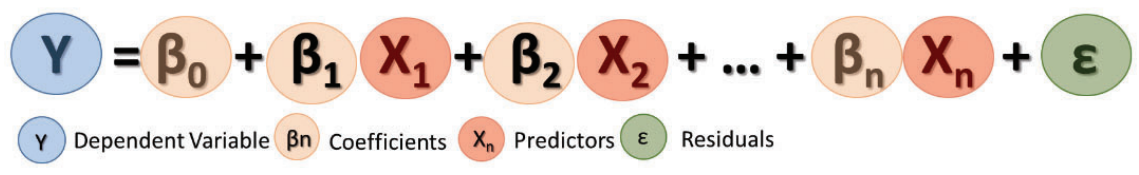
\includegraphics{images/RKequation.png}
\caption{Linear regression model}
\end{figure}

Before we proceed with the regression analysis, it is advisable to
inspect the histogram of the dependent/target variable, in order to see
if it needs to be transformed before fitting the regression model. The
data for the selected soil property is normal when the frequency
distribution of the values follow a bell-shaped curve (Gaussian
distribution) which is symmetric around its mean. Normality tests may be
used to assess normality. If a normality test indicates that data are
not normally distributed, it may be necessary to transform the data to
meet the normality assumption.

\begin{quote}
Both, the normality tests and the data transformation can be easily
performed using any commercial or open source statistical tool (R, SPSS,
MINITAB\ldots{})
\end{quote}

The main steps for the multiple linear regression analysis are shown in
the Figure \ref{fig:workflowRK}.

\begin{figure}

{\centering 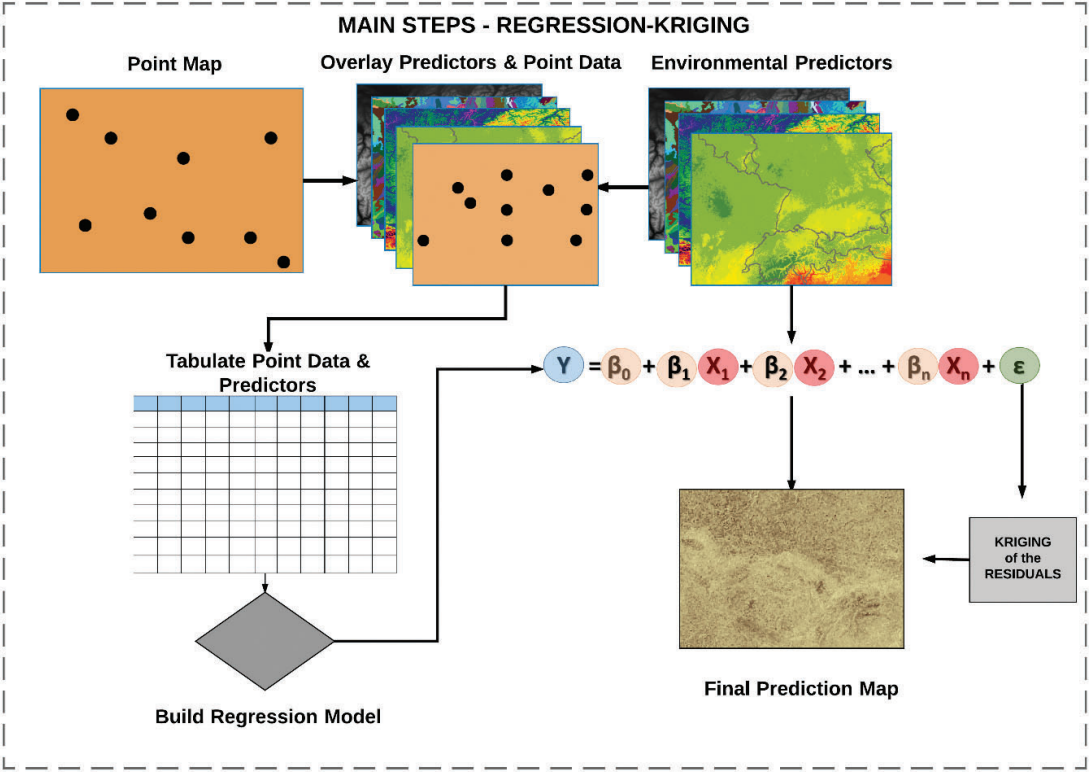
\includegraphics[width=0.8\linewidth]{images/RKworkflow} 

}

\caption{Workflow for Regression Kriging}\label{fig:workflowRK}
\end{figure}

\begin{quote}
\begin{enumerate}
\def\labelenumi{\arabic{enumi}.}
\tightlist
\item
  The first step is to prepare a map showing the spatial distribution of
  the sample locations and the corresponding soil property information,
  e.g.~soil organic matter and environmental properties. The first can
  be achieved as outlined in section
  \protect\hyperlink{overlay-covariates-and-spatial-data}{Overlay
  covariates and spatial data}. The overlaying operation can be
  performed in R, ArcGIS, SAGA GIS or QGIS.
\item
  The essential part of multiple regression analysis is to build a
  regression model by using the environmental predictors. After
  extracting the values of explanatory maps and target variables into
  the single table, we can now start fitting multiple regression model
  using the table that contains data from dependent variable and
  predictors.
\item
  In particular cases, stepwise multiple linear regression (SMLR) can be
  used to eliminate insignificant predictors. Stepwise multiple linear
  regression (SMLR) usually selects predictors that have the strongest
  linear correlations with the target variable, which reflect the
  highest predictive capacity.
\item
  Kriging of the residuals (prediction errors): In the
  regression-kriging, the regression model detrends the data, produces
  the residuals which we need to krige and to be added to the regression
  model predictions.
\end{enumerate}
\end{quote}

\hypertarget{interpret-the-key-results-of-multiple-regression}{%
\subsection{Interpret the Key Results of Multiple
Regression}\label{interpret-the-key-results-of-multiple-regression}}

Regression analysis generates an equation to describe the statistical
relationship between one or more predictor variables and the response
variable. he r-squared, p-values and coefficients that appear in the
output for linear regression analysis must also be reviewed. Before
accepting the result of a linear regression it is important to evaluate
its suitability at explaining the data. One of the many ways to do this
is to visually examine the residuals. If the model is appropriate, then
the residual errors should be random and normally distributed.

\textbf{R-sq}

R2 is the percentage of variation in the response that is explained by
the model. The higher the R2 Value, the better the model fits your data.
R-squared is always between \(0\%\) and \(100\%\). R2 usually increases
when additional predictors are added in the model.

\textbf{P Values}

To determine whether the association between the dependent and each
predictor in the model is statistically significant, compare the p-value
for the term to your significance level to assess the null hypothesis.
Usually, a significance level of 0.05 works well. P-value ≤ significance
level: The relationship is statistically significant. If the p-value is
less than or equal to the significance level, we can conclude that there
is a statistically significant relationship between the dependent
variable and the predictor. P-value \textgreater{} significance level:
The relationship is not statistically significant, If the p-value is
greater than the significance level, you cannot conclude that there is a
statistically significant relationship between the dependent variable
and the predictor. You may want to refit the model without the
predictor.

\textbf{Residuals}

We can plot the residuals which can help us determine whether the model
is adequate and meets the assumptions of the analysis. If the model is
appropriate, then the residual errors should be random and normally
distributed. We can plot residuals versus fits to verify the assumption
that the residuals are randomly distributed and have constant variance.
Ideally, the points should fall randomly on both sides of ``0'', with no
recognizable patterns in the points.

The diagnostic plots for the model should be evaluated to confirm if all
the assumptions of linear regression are met. After the abovementioned
assumptions are validated, we can proceed with making the prediction map
using the model with significant predictors.

\hypertarget{using-the-results-of-a-regression-analysis-to-make-predictions}{%
\subsection{Using the Results of a Regression Analysis to Make
Predictions}\label{using-the-results-of-a-regression-analysis-to-make-predictions}}

The purpose of a regression analysis, of course, is to develop a model
that can be used to make the prediction of a dependent variable. The
derived regression equation is to be used to create the prediction map
for the dependent variable.

\begin{quote}
Raster calculation can be easily performed using ``raster'' Package in R
or ArcGIS using the ''Raster Calculator'' tool (It's called Map Algebra
in the prior versions).
\end{quote}

\hypertarget{technical-steps---regression-kriging}{%
\subsection{Technical Steps - Regression
Kriging}\label{technical-steps---regression-kriging}}

\textbf{Requirements} The following are required to implement Regression
Kriging in R

\begin{itemize}
\item
  Setting-up the Software Environment
\item
  Obtaining and Installing R Studio
\item
  R Packages
\item
  Preparation of local soil property data
\item
  Preparation of spatial covariates

  \begin{itemize}
  \item
    DEM-derived covariates
  \item
    Land cover/Land use
  \item
    Climate
  \item
    Parent material
  \end{itemize}
\end{itemize}

\hypertarget{setting-working-space-and-initial-steps}{%
\subsubsection{Setting Working Space and Initial
Steps}\label{setting-working-space-and-initial-steps}}

One of the first steps should be setting our working directory. If you
read/write files from/ to disk, this takes place in the working
directory. If we don't set the working directory we could easily write
files to an undesirable file location. The following example shows how
to set the working directory in R to our folder which contains data for
the study area (point data, covariates).

Note that we must use the forward slash / or double backslash
\textbackslash{}\textbackslash{} in R! Single backslash \textbackslash{}
will not work. Now we can check if the working directory has been
correctly set by using the function:

\begin{Shaded}
\begin{Highlighting}[]
\KeywordTok{getwd}\NormalTok{()}
\end{Highlighting}
\end{Shaded}

\hypertarget{data-preparation-1}{%
\subsubsection{Data Preparation}\label{data-preparation-1}}

\textbf{Point Dataset}

We previously applied spline function to produce continuous soil
information to a given soil depth (0-30 cm) in section
\ref{EqualAreaSplines}. Spline function basically imports soil profile
data (including instances where layers are not contiguous), fits it to a
mass-preserving spline and outputs attribute means for a given depth.
The output file should contain profile id, upper (surface) and lower
depth (30cm), the estimated value for the selected soil attribute
(Value) and tmse (estimated mean squared error of the spline). If you
used the Spline Tool V2, the coordinates were not kept in the output
file. The coordinates should be added back in the data table. You can
use Profile IDs to add the X, Y columns back. Once your point dataset is
ready, copy this table into your working directory as a .csv file.

\textbf{Environmental Predictors (Covariates)}

In the Chapter \ref{covariates}, we presented and prepared several
global and continental datasets. In addition to these datasets, numerous
covariate layers have been prepared by ISRIC for the GSOC Map project.
These are GIS raster layers of various biophysical earth surface
properties for each country in the world. Some of these layers will be
used as predictors in this section. Please download the covariates for
your own study area from GSOCMap Data Repository as explained in section
\ref{GSOCDataRepo}.

In section \ref{overlay-soil-covariates}, a table with the points values
after data preparation and the values of our spatial predictors was
prepared. This step involves loading this table.

Now we will import our point dataset using \texttt{read.csv()} function.
The easiest way to create a data frame is to read in data from a
file---this is done using the function read.csv, which works with comma
delimited files. Data can be read in from other file formats as well,
using different functions, but read.csv is the most commonly used
approach. R is very flexible in how it reads in data from text files
(\texttt{read.table}, \texttt{read.csv}, \texttt{read.csv2},
\texttt{read.delim}, \texttt{read.delim2}). Please type
\texttt{?read.table()} for help.

\begin{Shaded}
\begin{Highlighting}[]
\CommentTok{# load data}
\NormalTok{dat <-}\StringTok{ }\KeywordTok{read.csv}\NormalTok{(}\StringTok{"data/MKD_RegMatrix.csv"}\NormalTok{)}

\NormalTok{dat}\OperatorTok{$}\NormalTok{LCEE10 <-}\StringTok{ }\KeywordTok{as.factor}\NormalTok{(dat}\OperatorTok{$}\NormalTok{LCEE10)}
\NormalTok{dat}\OperatorTok{$}\NormalTok{soilmap <-}\StringTok{ }\KeywordTok{as.factor}\NormalTok{(dat}\OperatorTok{$}\NormalTok{soilmap)}

\CommentTok{# explore the data structure}
\KeywordTok{str}\NormalTok{(dat)}
\end{Highlighting}
\end{Shaded}

\begin{verbatim}
## 'data.frame':    2897 obs. of  23 variables:
##  $ id       : Factor w/ 2897 levels "P0003","P0007",..: 1 2 3 4..
##  $ Y        : num  42 42 42.1 42 42 ...
##  $ X        : num  20.8 20.8 20.8 20.9 20.9 ...
##  $ SOC      : num  26.38 6.15 3.94 3.26 2.29 ...
##  $ BLD      : num  0.73 1.17 1.3 1.34 1.41 ...
##  $ CRFVOL   : num  8 18.6 31.9 21.7 14.5 ...
##  $ OCSKGM   : num  5.32 1.75 1.04 1.03 0.83 ...
##  $ meaERROR : num  2.16 2.85 2.65 3.16 3.63 2.83 2.94 2.49 2.77..
##  $ OCSKGMlog: num  1.6712 0.5591 0.0429 0.0286 -0.1862 ...
##  $ B04CHE3  : num  574 553 693 743 744 ...
##  $ B07CHE3  : num  38.5 37.8 42.1 43.7 43.7 ...
##  $ B13CHE3  : num  111.6 125 99.8 118.1 121 ...
##  $ B14CHE3  : num  59.2 60.3 42.4 39.9 38.7 ...
##  $ DEMENV5  : int  2327 2207 1243 1120 1098 1492 1413 1809 1731..
##  $ LCEE10   : Factor w/ 4 levels "1","2","3","4": 1 3 2 1 2 2 2..
##  $ PRSCHE3  : num  998 1053 780 839 844 ...
##  $ SLPMRG5  : int  13 36 6 25 30 24 15 17 20 43 ...
##  $ TMDMOD3  : int  282 280 285 288 289 287 286 286 287 286 ...
##  $ TMNMOD3  : int  272 270 277 279 279 277 277 273 274 273 ...
##  $ TWIMRG5  : int  61 62 81 66 65 72 68 67 65 59 ...
##  $ VBFMRG5  : int  0 0 14 0 0 0 0 0 0 0 ...
##  $ VDPMRG5  : int  311 823 10048 1963 -173 -400 -9 -692 -1139 2..
##  $ soilmap  : Factor w/ 20 levels "1","2","3","4",..: 6 14 14 3..
\end{verbatim}

Since we will be working with spatial data we need to define the
coordinates for the imported data. Using the coordinates() function from
the sp package we can define the columns in the data frame to refer to
spatial coordinates---here the coordinates are listed in columns X and
Y.

\begin{Shaded}
\begin{Highlighting}[]
\KeywordTok{library}\NormalTok{(sp)}

\CommentTok{# Promote to spatialPointsDataFrame}
\KeywordTok{coordinates}\NormalTok{(dat) <-}\StringTok{ }\ErrorTok{~}\StringTok{ }\NormalTok{X }\OperatorTok{+}\StringTok{ }\NormalTok{Y}

\KeywordTok{class}\NormalTok{(dat)}
\end{Highlighting}
\end{Shaded}

\begin{verbatim}
## [1] "SpatialPointsDataFrame"
## attr(,"package")
## [1] "sp"
\end{verbatim}

SpatialPointsDataFrame structure is essentially the same data frame,
except that additional ``spatial'' elements have been added or
partitioned into slots. Some important ones being the bounding box (sort
of like the spatial extent of the data), and the coordinate reference
system proj4string(), which we need to define for the sample dataset. To
define the CRS, we must know where our data are from, and what was the
corresponding CRS used when recording the spatial information in the
field. For this data set, the CRS used was: WGS84 (EPSG:4326).

To clearly tell R this information we define the CRS which describes a
reference system in a way understood by the
\href{http://trac.osgeo.org/proj/}{PROJ.4 projection library}. An
interface to the PROJ.4 library is available in the rgdal package. As an
alternative to using Proj4 character strings, we can use the
corresponding yet simpler EPSG code (European Petroleum Survey Group).
rgdal also recognizes these codes. If you are unsure of the Proj4 or
EPSG code for the spatial data that you have but know the CRS, you
should consult \url{http://spatialreference.org/} for assistance.

Please also note that, when working with spatial data, it's very
important that the CRS (coordinate reference system) of the point data
and covariates are the same.

Now, we will define our CRS:

\begin{Shaded}
\begin{Highlighting}[]
\NormalTok{dat}\OperatorTok{@}\NormalTok{proj4string <-}\StringTok{ }\KeywordTok{CRS}\NormalTok{(}\DataTypeTok{projargs =} \StringTok{"+init=epsg:4326"}\NormalTok{)}

\NormalTok{dat}\OperatorTok{@}\NormalTok{proj4string}
\end{Highlighting}
\end{Shaded}

\begin{verbatim}
## CRS arguments:
##  +init=epsg:4326 +proj=longlat +datum=WGS84 +no_defs
## +ellps=WGS84 +towgs84=0,0,0
\end{verbatim}

Now we will import the covariates. When the covariate layers are in
common resolution and extent, rather than working with individual
rasters it is better to stack them all into a single R object. In this
example, we use 13 covariates from the GSOCMap Data Repository and a
rasterized version of the soil type map. The rasterization of vectorial
data was covered in
\protect\hyperlink{technical-steps---rasterizing-a-vector-layer-in-r}{Technical
Steps - Rasterizing a vector layer in R}. The file containing all the
covariates was prepared at the end of chapter \ref{covariates}.

\begin{Shaded}
\begin{Highlighting}[]
\KeywordTok{load}\NormalTok{(}\DataTypeTok{file =} \StringTok{"covariates.RData"}\NormalTok{)}

\KeywordTok{names}\NormalTok{(covs)}
\end{Highlighting}
\end{Shaded}

\begin{verbatim}
##  [1] "B04CHE3" "B07CHE3" "B13CHE3" "B14CHE3" "DEMENV5" "LCEE10" 
##  [7] "PRSCHE3" "SLPMRG5" "TMDMOD3" "TMNMOD3" "TWIMRG5" "VBFMRG5"
## [13] "VDPMRG5" "soilmap"
\end{verbatim}

\hypertarget{fitting-the-mlr-model}{%
\subsubsection{Fitting the MLR Model}\label{fitting-the-mlr-model}}

\textbf{Fitting the MLR Model}

It would be better to progress with a data frame of just the data and
covariates required for the modeling. In this case, we will subset the
columns SOC, the covariates and the spatial coordinates (X and Y).

\begin{Shaded}
\begin{Highlighting}[]
\NormalTok{datdf <-}\StringTok{ }\NormalTok{dat}\OperatorTok{@}\NormalTok{data}

\NormalTok{datdf <-}\StringTok{ }\NormalTok{datdf[, }\KeywordTok{c}\NormalTok{(}\StringTok{"OCSKGM"}\NormalTok{, }\KeywordTok{names}\NormalTok{(covs))]}
\end{Highlighting}
\end{Shaded}

Let's fit a linear model using with all available covariates.

\begin{Shaded}
\begin{Highlighting}[]
\CommentTok{# Fit a multiple linear regression model between the log transformed}
\CommentTok{# values of OCS and the top 20 covariates}
\NormalTok{model.MLR <-}\StringTok{ }\KeywordTok{lm}\NormalTok{(}\KeywordTok{log}\NormalTok{(OCSKGM) }\OperatorTok{~}\StringTok{ }\NormalTok{., }\DataTypeTok{data =}\NormalTok{ datdf)}
\end{Highlighting}
\end{Shaded}

From the summary of our fitted model (model.MLR) above, it seems only a
few of the covariates are significant in describing the spatial
variation of the target variable. To determine the most predictive model
we can run a stepwise regression using the \texttt{step()} function.
With this function, we can also specify the mode of stepwise search, can
be one of ``both'', ``backward'', or ``forward''.

\begin{Shaded}
\begin{Highlighting}[]
\NormalTok{## stepwise variable selection}
\NormalTok{model.MLR.step <-}\StringTok{ }\KeywordTok{step}\NormalTok{(model.MLR, }\DataTypeTok{direction=}\StringTok{"both"}\NormalTok{)}
\end{Highlighting}
\end{Shaded}

Comparing the summary of both the full and stepwise linear models, there
is very little difference between the models such as the R2. Both models
explain about \(23\%\) of variation of the target variable. Obviously,
the ``full'' model is more complex as it has more parameters than the
``step'' model.

\begin{Shaded}
\begin{Highlighting}[]
\CommentTok{# summary and anova of the new model using stepwise covariates}
\CommentTok{# selection}
\KeywordTok{summary}\NormalTok{(model.MLR.step)}
\KeywordTok{anova}\NormalTok{(model.MLR.step)}
\end{Highlighting}
\end{Shaded}

\begin{verbatim}
## 
## Call:
## lm(formula = log(OCSKGM) ~ B04CHE3 + B07CHE3 + B13CHE3 + DEMENV5 + 
##     LCEE10 + PRSCHE3 + SLPMRG5 + TMDMOD3 + TMNMOD3 + VBFMRG5 + 
##     VDPMRG5 + soilmap, data = datdf)
## 
## Residuals:
##     Min      1Q  Median      3Q     Max 
## -3.3625 -0.2637  0.0368  0.3111  1.8859 
## 
## Coefficients:
##               Estimate Std. Error t value Pr(>|t|)    
## (Intercept)  9.166e+00  4.343e+00   2.111  0.03489 *  
## B04CHE3     -5.877e-03  1.099e-03  -5.347 9.64e-08 ***
## B07CHE3      1.110e-01  3.460e-02   3.209  0.00135 ** 
## B13CHE3     -4.361e-03  1.640e-03  -2.659  0.00788 ** 
## DEMENV5     -1.882e-04  8.926e-05  -2.108  0.03508 *  
## LCEE102      9.745e-02  3.369e-02   2.893  0.00385 ** 
## LCEE103      1.399e-01  5.490e-02   2.548  0.01088 *  
## LCEE104     -3.612e-02  4.360e-02  -0.829  0.40741    
## PRSCHE3      9.174e-04  3.139e-04   2.923  0.00350 ** 
## SLPMRG5     -2.440e-03  1.508e-03  -1.619  0.10559    
## TMDMOD3     -5.584e-02  7.612e-03  -7.336 2.86e-13 ***
## TMNMOD3      2.467e-02  1.291e-02   1.911  0.05611 .  
## VBFMRG5      4.941e-04  9.867e-05   5.008 5.84e-07 ***
## VDPMRG5     -2.696e-05  4.360e-06  -6.185 7.11e-10 ***
## soilmap2    -3.848e-01  4.885e-01  -0.788  0.43090    
## soilmap3    -2.094e-01  4.825e-01  -0.434  0.66429    
## soilmap4    -1.955e-01  4.886e-01  -0.400  0.68919    
## soilmap5    -6.323e-02  5.202e-01  -0.122  0.90327    
## soilmap6     2.087e-01  4.841e-01   0.431  0.66649    
## soilmap7     1.459e-01  4.857e-01   0.300  0.76398    
## soilmap8    -1.875e-01  4.848e-01  -0.387  0.69904    
## soilmap9    -3.278e-01  4.817e-01  -0.681  0.49617    
## soilmap10   -1.001e-01  4.833e-01  -0.207  0.83590    
## soilmap11   -3.587e-01  4.874e-01  -0.736  0.46188    
## soilmap12   -2.135e-01  4.822e-01  -0.443  0.65797    
## soilmap13    3.091e-01  5.563e-01   0.556  0.57855    
## soilmap14   -2.224e-01  4.828e-01  -0.461  0.64506    
## soilmap15   -1.905e-01  4.876e-01  -0.391  0.69600    
## soilmap16   -3.482e-01  4.831e-01  -0.721  0.47112    
## soilmap17   -1.478e-01  4.838e-01  -0.306  0.75996    
## soilmap18   -8.714e-02  4.830e-01  -0.180  0.85684    
## soilmap19   -5.491e-01  5.082e-01  -1.080  0.28002    
## soilmap20   -3.123e-01  4.846e-01  -0.644  0.51934    
## ---
## Signif. codes:  0 '***' 0.001 '**' 0.01 '*' 0.05 '.' 0.1 ' ' 1
## 
## Residual standard error: 0.4806 on 2864 degrees of freedom
## Multiple R-squared:  0.2472, Adjusted R-squared:  0.2388 
## F-statistic: 29.38 on 32 and 2864 DF,  p-value: < 2.2e-16
## 
## Analysis of Variance Table
## 
## Response: log(OCSKGM)
##             Df Sum Sq Mean Sq  F value    Pr(>F)    
## B04CHE3      1 111.35 111.347 482.0082 < 2.2e-16 ***
## B07CHE3      1   2.33   2.335  10.1060  0.001494 ** 
## B13CHE3      1   1.64   1.642   7.1059  0.007726 ** 
## DEMENV5      1   5.07   5.067  21.9339 2.953e-06 ***
## LCEE10       3  17.22   5.740  24.8497 7.201e-16 ***
## PRSCHE3      1   4.91   4.910  21.2530 4.201e-06 ***
## SLPMRG5      1   1.97   1.971   8.5305  0.003520 ** 
## TMDMOD3      1   3.75   3.749  16.2300 5.756e-05 ***
## TMNMOD3      1   0.60   0.602   2.6081  0.106428    
## VBFMRG5      1  12.75  12.750  55.1943 1.433e-13 ***
## VDPMRG5      1  10.80  10.797  46.7375 9.880e-12 ***
## soilmap     19  44.83   2.359  10.2135 < 2.2e-16 ***
## Residuals 2864 661.60   0.231                       
## ---
## Signif. codes:  0 '***' 0.001 '**' 0.01 '*' 0.05 '.' 0.1 ' ' 1
\end{verbatim}

In those two models above, we used all available points. It is important
to test the performance of a model based upon an external validation.
Let's fit a new model using a random subset of the available data. We
will sample \(70\%\) of the SOC data for the model calibration data set.

\begin{Shaded}
\begin{Highlighting}[]
\CommentTok{# graphical diagnosis of the regression analysis}
\KeywordTok{par}\NormalTok{(}\DataTypeTok{mfrow=}\KeywordTok{c}\NormalTok{(}\DecValTok{2}\NormalTok{,}\DecValTok{2}\NormalTok{))}
\KeywordTok{plot}\NormalTok{(model.MLR.step)}
\end{Highlighting}
\end{Shaded}

\begin{verbatim}
## Warning: not plotting observations with leverage one:
##   340

## Warning: not plotting observations with leverage one:
##   340
\end{verbatim}

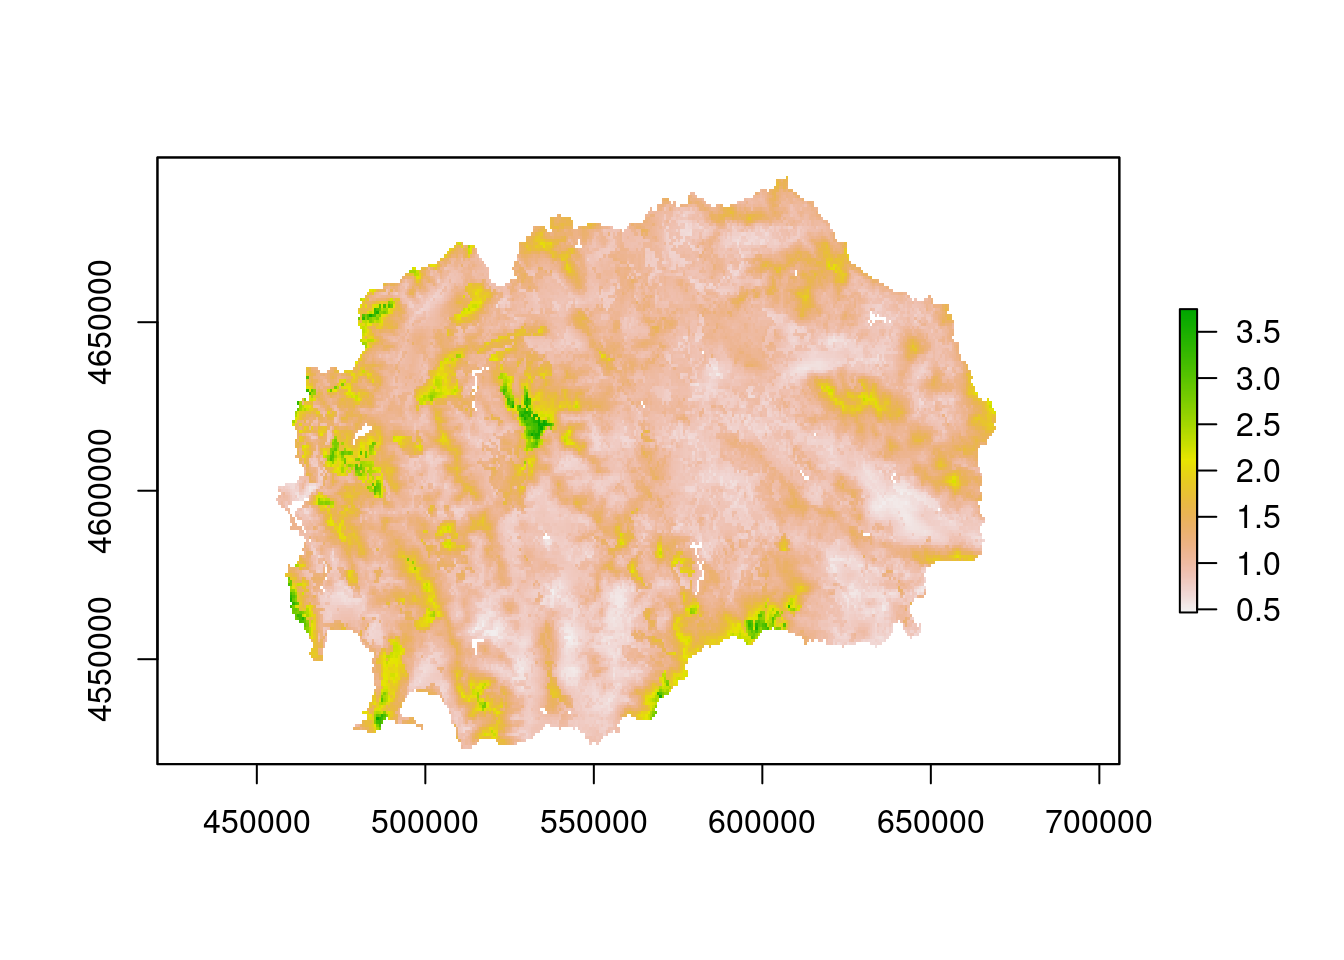
\includegraphics{SOCMapping_files/figure-latex/unnamed-chunk-41-1.pdf}

\begin{Shaded}
\begin{Highlighting}[]
\KeywordTok{par}\NormalTok{(}\DataTypeTok{mfrow=}\KeywordTok{c}\NormalTok{(}\DecValTok{1}\NormalTok{,}\DecValTok{1}\NormalTok{))}
\end{Highlighting}
\end{Shaded}

\begin{Shaded}
\begin{Highlighting}[]
\CommentTok{# collinearity test using variance inflation factors}
\KeywordTok{library}\NormalTok{(car)}
\KeywordTok{vif}\NormalTok{(model.MLR.step)}
\end{Highlighting}
\end{Shaded}

\begin{verbatim}
##              GVIF Df GVIF^(1/(2*Df))
## B04CHE3 17.352988  1        4.165692
## B07CHE3 17.580993  1        4.192969
## B13CHE3 14.463943  1        3.803149
## DEMENV5 14.325207  1        3.784866
## LCEE10   3.349841  3        1.223219
## PRSCHE3 20.323563  1        4.508166
## SLPMRG5  3.201225  1        1.789197
## TMDMOD3  6.724708  1        2.593204
## TMNMOD3  6.172634  1        2.484479
## VBFMRG5  4.182605  1        2.045142
## VDPMRG5  1.933334  1        1.390444
## soilmap 16.784795 19        1.077047
\end{verbatim}

\begin{Shaded}
\begin{Highlighting}[]
\CommentTok{# problematic covariates should have sqrt(VIF) > 2}
\KeywordTok{sqrt}\NormalTok{(}\KeywordTok{vif}\NormalTok{(model.MLR.step))}
\end{Highlighting}
\end{Shaded}

\begin{verbatim}
##             GVIF       Df GVIF^(1/(2*Df))
## B04CHE3 4.165692 1.000000        2.041003
## B07CHE3 4.192969 1.000000        2.047674
## B13CHE3 3.803149 1.000000        1.950166
## DEMENV5 3.784866 1.000000        1.945473
## LCEE10  1.830257 1.732051        1.105992
## PRSCHE3 4.508166 1.000000        2.123244
## SLPMRG5 1.789197 1.000000        1.337609
## TMDMOD3 2.593204 1.000000        1.610343
## TMNMOD3 2.484479 1.000000        1.576223
## VBFMRG5 2.045142 1.000000        1.430085
## VDPMRG5 1.390444 1.000000        1.179171
## soilmap 4.096925 4.358899        1.037809
\end{verbatim}

colinear: Temperature seasonality at 1 km (B04CHE3) and Temperature
Annual Range {[}°C{]} at 1 km (B07CHE3)

\begin{Shaded}
\begin{Highlighting}[]
\CommentTok{# Removing B07CHE3 from the stepwise model:}
\NormalTok{model.MLR.step <-}\StringTok{ }\KeywordTok{update}\NormalTok{(model.MLR.step, . }\OperatorTok{~}\StringTok{ }\NormalTok{. }\OperatorTok{-}\StringTok{ }\NormalTok{B07CHE3)}

\CommentTok{# Test the vif again:}
\KeywordTok{sqrt}\NormalTok{(}\KeywordTok{vif}\NormalTok{(model.MLR.step))}
\end{Highlighting}
\end{Shaded}

\begin{verbatim}
##             GVIF       Df GVIF^(1/(2*Df))
## B04CHE3 2.268418 1.000000        1.506127
## B13CHE3 3.624615 1.000000        1.903842
## DEMENV5 3.645817 1.000000        1.909402
## LCEE10  1.818077 1.732051        1.104762
## PRSCHE3 4.460815 1.000000        2.112064
## SLPMRG5 1.783090 1.000000        1.335324
## TMDMOD3 2.572322 1.000000        1.603846
## TMNMOD3 2.299838 1.000000        1.516522
## VBFMRG5 2.015123 1.000000        1.419550
## VDPMRG5 1.387165 1.000000        1.177780
## soilmap 3.840284 4.358899        1.036043
\end{verbatim}

\begin{Shaded}
\begin{Highlighting}[]
\CommentTok{# summary  of the new model using stepwise covariates selection}
\KeywordTok{summary}\NormalTok{(model.MLR.step)}
\end{Highlighting}
\end{Shaded}

\begin{verbatim}
## 
## Call:
## lm(formula = log(OCSKGM) ~ B04CHE3 + B13CHE3 + DEMENV5 + LCEE10 + 
##     PRSCHE3 + SLPMRG5 + TMDMOD3 + TMNMOD3 + VBFMRG5 + VDPMRG5 + 
##     soilmap, data = datdf)
## 
## Residuals:
##     Min      1Q  Median      3Q     Max 
## -3.3857 -0.2662  0.0390  0.3096  1.9418 
## 
## Coefficients:
##               Estimate Std. Error t value Pr(>|t|)    
## (Intercept)  1.536e+01  3.896e+00   3.943 8.23e-05 ***
## B04CHE3     -2.919e-03  5.994e-04  -4.869 1.18e-06 ***
## B13CHE3     -5.955e-03  1.566e-03  -3.804 0.000146 ***
## DEMENV5     -2.651e-04  8.612e-05  -3.079 0.002099 ** 
## LCEE102      1.006e-01  3.373e-02   2.983 0.002879 ** 
## LCEE103      1.250e-01  5.479e-02   2.281 0.022598 *  
## LCEE104     -2.756e-02  4.358e-02  -0.632 0.527224    
## PRSCHE3      1.063e-03  3.111e-04   3.417 0.000642 ***
## SLPMRG5     -2.041e-03  1.505e-03  -1.356 0.175085    
## TMDMOD3     -5.275e-02  7.563e-03  -6.974 3.80e-12 ***
## TMNMOD3      8.998e-03  1.197e-02   0.752 0.452305    
## VBFMRG5      4.401e-04  9.738e-05   4.519 6.47e-06 ***
## VDPMRG5     -2.792e-05  4.357e-06  -6.410 1.70e-10 ***
## soilmap2    -4.166e-01  4.892e-01  -0.852 0.394494    
## soilmap3    -1.925e-01  4.832e-01  -0.398 0.690372    
## soilmap4    -1.959e-01  4.894e-01  -0.400 0.688957    
## soilmap5    -6.440e-02  5.211e-01  -0.124 0.901641    
## soilmap6     2.098e-01  4.849e-01   0.433 0.665224    
## soilmap7     1.337e-01  4.865e-01   0.275 0.783490    
## soilmap8    -1.838e-01  4.856e-01  -0.379 0.705074    
## soilmap9    -3.376e-01  4.825e-01  -0.700 0.484097    
## soilmap10   -9.951e-02  4.841e-01  -0.206 0.837162    
## soilmap11   -3.570e-01  4.882e-01  -0.731 0.464661    
## soilmap12   -2.104e-01  4.830e-01  -0.436 0.663172    
## soilmap13    2.675e-01  5.570e-01   0.480 0.631148    
## soilmap14   -2.312e-01  4.836e-01  -0.478 0.632615    
## soilmap15   -1.733e-01  4.883e-01  -0.355 0.722668    
## soilmap16   -3.620e-01  4.839e-01  -0.748 0.454464    
## soilmap17   -1.564e-01  4.846e-01  -0.323 0.746854    
## soilmap18   -6.759e-02  4.837e-01  -0.140 0.888886    
## soilmap19   -5.479e-01  5.090e-01  -1.076 0.281873    
## soilmap20   -3.061e-01  4.853e-01  -0.631 0.528351    
## ---
## Signif. codes:  0 '***' 0.001 '**' 0.01 '*' 0.05 '.' 0.1 ' ' 1
## 
## Residual standard error: 0.4814 on 2865 degrees of freedom
## Multiple R-squared:  0.2445, Adjusted R-squared:  0.2363 
## F-statistic:  29.9 on 31 and 2865 DF,  p-value: < 2.2e-16
\end{verbatim}

\begin{Shaded}
\begin{Highlighting}[]
\CommentTok{# outlier test using the Bonferroni test}
\KeywordTok{outlierTest}\NormalTok{(model.MLR.step)}
\end{Highlighting}
\end{Shaded}

\begin{verbatim}
##       rstudent unadjusted p-value Bonferonni p
## 1967 -7.114604         1.4122e-12   4.0897e-09
## 705  -6.795188         1.3108e-11   3.7959e-08
## 1154 -6.045856         1.6789e-09   4.8621e-06
## 1395 -5.112379         3.3907e-07   9.8194e-04
## 709  -5.078342         4.0515e-07   1.1733e-03
## 1229 -4.842237         1.3520e-06   3.9155e-03
## 1136 -4.468410         8.1860e-06   2.3707e-02
\end{verbatim}

\hypertarget{prediction-and-residual-kriging}{%
\subsubsection{Prediction and Residual
Kriging}\label{prediction-and-residual-kriging}}

Now we can make the predictions and plot the map. We can use either our
DSM\_data table for covariate values or \texttt{covs} object for making
our prediction. Using stack avoids the step of arranging all covariates
into a table format. If multiple rasters are being used, it is necessary
to have them arranged as a rasterStack object. This is useful as it also
ensures all the rasters are of the same extent and resolution. Here we
can use the raster predict function such as below using the covStack
raster stack as we created in the Step 3.

\begin{Shaded}
\begin{Highlighting}[]
\CommentTok{# Project point data.}
\NormalTok{dat <-}\StringTok{ }\KeywordTok{spTransform}\NormalTok{(dat, }\KeywordTok{CRS}\NormalTok{(}\StringTok{"+init=epsg:6204"}\NormalTok{))}

\CommentTok{# project covariates to VN-2000 UTM 48N}
\NormalTok{covs <-}\StringTok{ }\KeywordTok{projectRaster}\NormalTok{(covs, }\DataTypeTok{crs =} \KeywordTok{CRS}\NormalTok{(}\StringTok{"+init=epsg:6204"}\NormalTok{),}
                      \DataTypeTok{method=}\StringTok{'ngb'}\NormalTok{)}

\NormalTok{covs}\OperatorTok{$}\NormalTok{LCEE10 <-}\StringTok{ }\KeywordTok{as.factor}\NormalTok{(covs}\OperatorTok{$}\NormalTok{LCEE10)}
\NormalTok{covs}\OperatorTok{$}\NormalTok{soilmap <-}\StringTok{ }\KeywordTok{as.factor}\NormalTok{(covs}\OperatorTok{$}\NormalTok{soilmap)}
\end{Highlighting}
\end{Shaded}

\begin{Shaded}
\begin{Highlighting}[]
\CommentTok{# Promote covariates to spatial grid dataframe. Takes some time and}
\CommentTok{# a lot of memory!}
\NormalTok{covs.sp <-}\StringTok{ }\KeywordTok{as}\NormalTok{(covs, }\StringTok{"SpatialGridDataFrame"}\NormalTok{)}
\NormalTok{covs.sp}\OperatorTok{$}\NormalTok{LCEE10 <-}\StringTok{ }\KeywordTok{as.factor}\NormalTok{(covs.sp}\OperatorTok{$}\NormalTok{LCEE10)}
\NormalTok{covs.sp}\OperatorTok{$}\NormalTok{soilmap <-}\StringTok{ }\KeywordTok{as.factor}\NormalTok{(covs.sp}\OperatorTok{$}\NormalTok{soilmap)}
\end{Highlighting}
\end{Shaded}

\begin{verbatim}
## Checking if any bins have less than 5 points, merging bins when necessary...
## 
## Selected:
##   model      psill    range
## 1   Nug 0.16735323    0.000
## 2   Sph 0.06746394 6646.127
## 
## Tested models, best first:
##    Tested.models kappa      SSerror
## 1            Sph     0 3.964233e-07
## 25           Ste    10 4.182590e-07
## 24           Ste     5 4.266696e-07
## 23           Ste     2 4.501717e-07
## 22           Ste   1.9 4.519816e-07
## 21           Ste   1.8 4.539405e-07
## 20           Ste   1.7 4.560649e-07
## 19           Ste   1.6 4.583753e-07
## 18           Ste   1.5 4.608930e-07
## 17           Ste   1.4 4.636455e-07
## 16           Ste   1.3 4.666616e-07
## 3            Gau     0 4.680499e-07
## 15           Ste   1.2 4.699776e-07
## 14           Ste   1.1 4.736337e-07
## 13           Ste     1 4.776785e-07
## 12           Ste   0.9 4.821684e-07
## 11           Ste   0.8 4.871689e-07
## 10           Ste   0.7 4.927610e-07
## 9            Ste   0.6 4.990387e-07
## 2            Exp     0 5.061150e-07
## 8            Ste   0.5 5.061153e-07
## 7            Ste   0.4 5.141265e-07
## 6            Ste   0.3 5.232363e-07
## 5            Ste   0.2 5.336428e-07
## 4            Ste  0.05 1.148336e-06
## [using universal kriging]
\end{verbatim}

\begin{Shaded}
\begin{Highlighting}[]
\NormalTok{### RK model}
\KeywordTok{library}\NormalTok{(automap)}


\NormalTok{## Run regression kriging prediction. This step can take hours...!}
\NormalTok{OCS.krige <-}\StringTok{ }\KeywordTok{autoKrige}\NormalTok{(}\DataTypeTok{formula =}
                         \KeywordTok{as.formula}\NormalTok{(model.MLR.step}\OperatorTok{$}\NormalTok{call}\OperatorTok{$}\NormalTok{formula),}
                       \DataTypeTok{input_data =}\NormalTok{ dat,}
                       \DataTypeTok{new_data =}\NormalTok{ covs.sp,}
                       \DataTypeTok{verbose =} \OtherTok{TRUE}\NormalTok{,}
                       \DataTypeTok{block =} \KeywordTok{c}\NormalTok{(}\DecValTok{1000}\NormalTok{, }\DecValTok{1000}\NormalTok{))}

\NormalTok{OCS.krige}
\end{Highlighting}
\end{Shaded}

\begin{Shaded}
\begin{Highlighting}[]
\NormalTok{## Convert prediction and standard deviation to rasters}
\NormalTok{## And back-tansform the vlaues}
\NormalTok{RKprediction <-}\StringTok{ }\KeywordTok{exp}\NormalTok{(}\KeywordTok{raster}\NormalTok{(OCS.krige}\OperatorTok{$}\NormalTok{krige_output[}\DecValTok{1}\NormalTok{]))}
\NormalTok{RKpredsd <-}\StringTok{ }\KeywordTok{exp}\NormalTok{(}\KeywordTok{raster}\NormalTok{(OCS.krige}\OperatorTok{$}\NormalTok{krige_output[}\DecValTok{3}\NormalTok{]))}
\end{Highlighting}
\end{Shaded}

\begin{Shaded}
\begin{Highlighting}[]
\KeywordTok{plot}\NormalTok{(RKprediction)}
\end{Highlighting}
\end{Shaded}

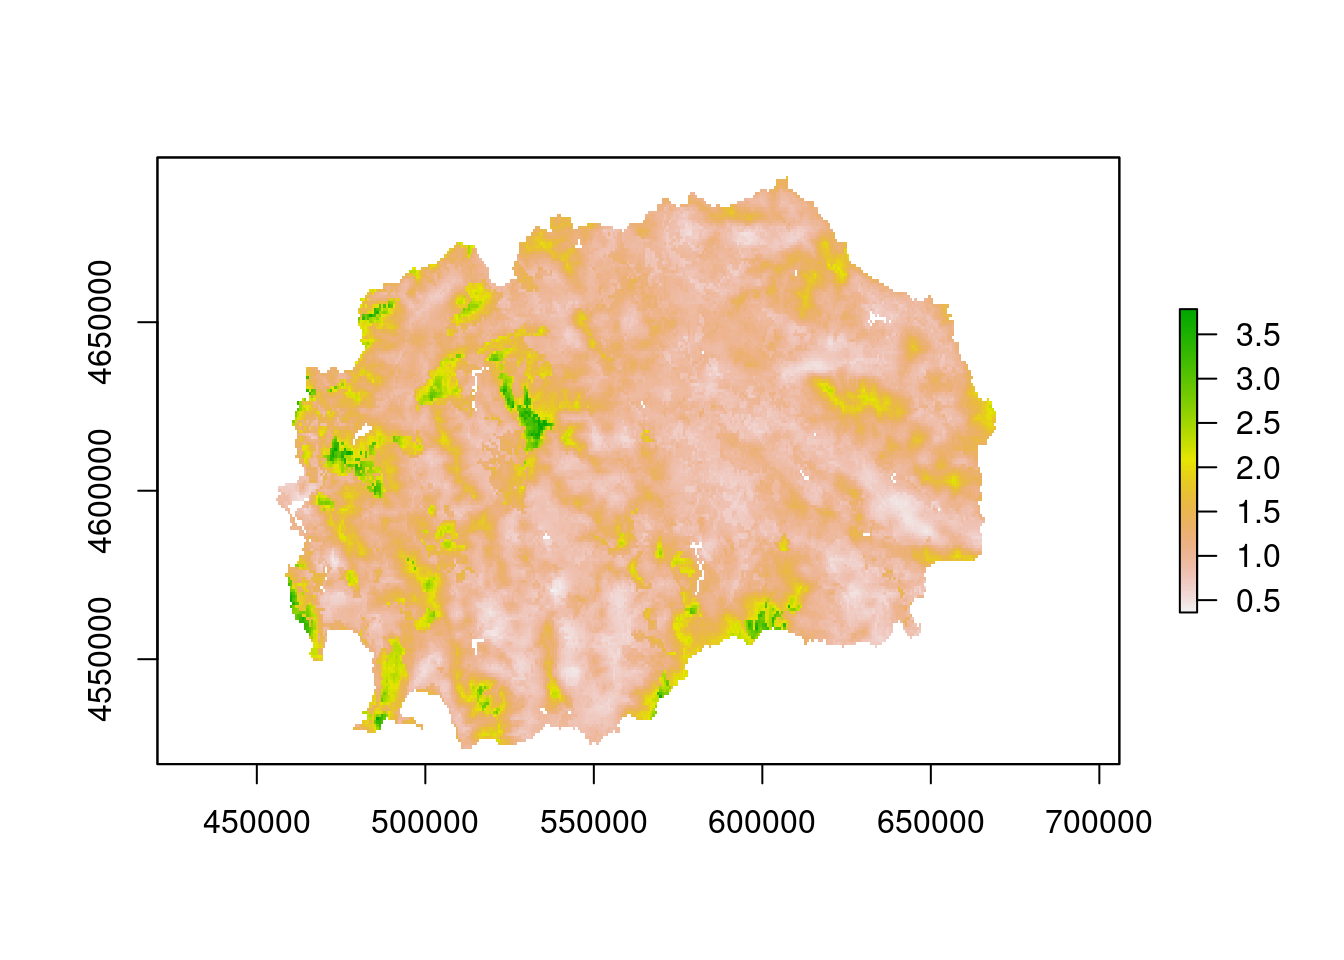
\includegraphics{SOCMapping_files/figure-latex/unnamed-chunk-49-1.pdf}

\begin{Shaded}
\begin{Highlighting}[]
\KeywordTok{plot}\NormalTok{(RKpredsd)}
\end{Highlighting}
\end{Shaded}

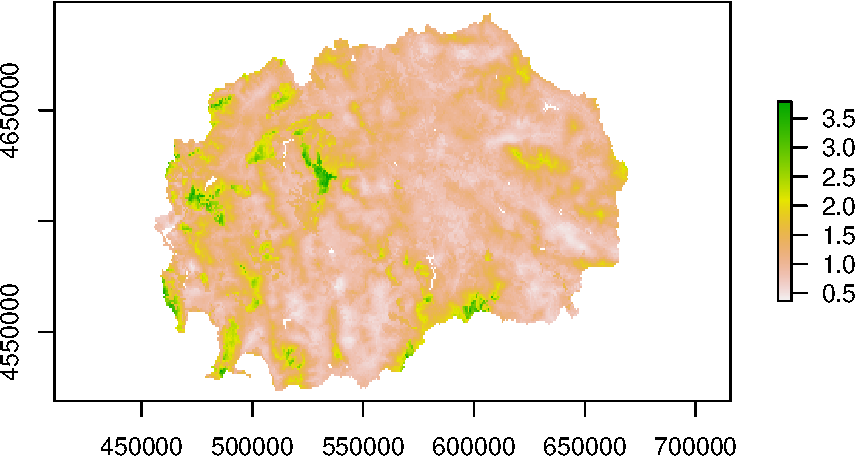
\includegraphics{SOCMapping_files/figure-latex/unnamed-chunk-50-1.pdf}

\begin{Shaded}
\begin{Highlighting}[]
\NormalTok{## Save results as tif files}
\KeywordTok{writeRaster}\NormalTok{(RKprediction, }\DataTypeTok{filename =} \StringTok{"results/MKD_OCSKGM_RK.tif"}\NormalTok{,}
            \DataTypeTok{overwrite =} \OtherTok{TRUE}\NormalTok{)}

\KeywordTok{writeRaster}\NormalTok{(RKpredsd, }\DataTypeTok{filename =} \StringTok{"results/MKD_OCSKGM_RKpredsd.tif"}\NormalTok{,}
            \DataTypeTok{overwrite =} \OtherTok{TRUE}\NormalTok{)}
\end{Highlighting}
\end{Shaded}

\begin{Shaded}
\begin{Highlighting}[]
\CommentTok{# save the model}
\KeywordTok{saveRDS}\NormalTok{(model.MLR.step, }\DataTypeTok{file=}\StringTok{"results/RKmodel.Rds"}\NormalTok{)}
\end{Highlighting}
\end{Shaded}

\hypertarget{technical-steps---cross-validation-of-regression-kriging-models}{%
\subsection{Technical Steps - Cross-validation of Regression Kriging
models}\label{technical-steps---cross-validation-of-regression-kriging-models}}

Cross-validation is introduced in Section \ref{xval}. In
Regression-Kriging models, n-fold cross-validation and leave-one-out
cross-validation can be run using the \texttt{krige.cv()} included in
**gstat* R package. In this example, we will apply 10 fold
cross-validation to our RK model.

\begin{Shaded}
\begin{Highlighting}[]
\CommentTok{# autoKrige.cv() does not removes the duplicated points}
\CommentTok{# we have to do it manually before running the cross-validation}
\NormalTok{dat =}\StringTok{ }\NormalTok{dat[}\KeywordTok{which}\NormalTok{(}\OperatorTok{!}\KeywordTok{duplicated}\NormalTok{(dat}\OperatorTok{@}\NormalTok{coords)), ]}

\NormalTok{OCS.krige.cv <-}\StringTok{ }\KeywordTok{autoKrige.cv}\NormalTok{(}\DataTypeTok{formula =} 
                            \KeywordTok{as.formula}\NormalTok{(model.MLR.step}\OperatorTok{$}\NormalTok{call}\OperatorTok{$}\NormalTok{formula), }
                             \DataTypeTok{input_data =}\NormalTok{ dat, }\DataTypeTok{nfold =} \DecValTok{10}\NormalTok{)}
\end{Highlighting}
\end{Shaded}

\begin{Shaded}
\begin{Highlighting}[]
\KeywordTok{summary}\NormalTok{(OCS.krige.cv)}
\end{Highlighting}
\end{Shaded}

\begin{verbatim}
##             [,1]    
## mean_error  0.004726
## me_mean     -0.3918 
## MAE         0.3402  
## MSE         0.2692  
## MSNE        0.9504  
## cor_obspred 0.4471  
## cor_predres -0.3132 
## RMSE        0.5188  
## RMSE_sd     0.9418  
## URMSE       0.5188  
## iqr         0.5223
\end{verbatim}

\clearpage

\hypertarget{rf}{%
\section{Data mining: Random Forest}\label{rf}}

\emph{M Guevara, C Thine, GF Olmedo \& RR Vargas}

\hypertarget{overview-2}{%
\subsection{Overview}\label{overview-2}}

Data mining uses different forms of statistics, such as machine
learning, to explore data matrices for a particular situation, from
specific information sources, and with a specific objective. Data mining
is used in digital soil mapping frameworks to generate spatial and
temporal predictions of soil properties or classes in places where no
information is available. Under a data mining-based digital soil mapping
framework, the exploration of statistical relationships (linear and
non-linear) between soil observational data and soil environmental
predictors is generally performed by the means of machine learning.
Machine learning methods represent a branch of statistics that can be
used to automatically extract information from available data, including
the non-linear and hidden relationships of high dimensional spaces or
hyper-volumes of information when high performance or distributed
computing resources are available. Machine learning methods do not rely
on statistical assumptions about the spatial structure of soil
variability or the empirical relationship of soil available data and its
environmental predictors. Therefore machine learning methods are also
suitable for digital soil mapping under limited and sparse scenarios of
data availability, although in practice the statistical performance of
machine learning (or any statistical method) is reduced by a low
representativeness of a soil property or class in the statistical space
given available data. Machine learning methods can be used for
(supervised and unsupervised) regression (e.g., predicting soil organic
carbon) or classification (e.g., predicting soil type classes) on
digital soil mapping. Machine learning methods can be roughly divided
into four main groups: linear-based (e.g., multiple linear regression),
kernel-based (e.g., kernel weighted nearest neighbors or support vector
machines), probabilistic-based (e.g., Bayesian statistics) and
tree-based (e.g., classification and regression trees). Random forest is
a tree-based machine learning algorithm that is popular on digital soil
mapping because it has proven to be efficient mapping soil properties
across a wide range of data scenarios and scales of soil variability.
Random forest can be implemented using open source platforms and this
chapter is devoted to provide a reproducible example of this machine
learning algorithm applied to soil organic carbon mapping across
Macedonia.

\hypertarget{random-forests}{%
\subsection{Random forests}\label{random-forests}}

Random forest is a Decision-tree-based machine learning method used in
digital soil mapping for uncovering the statistical relationship between
a dependent variable (e.g., soil property) and its predictors.
Decision-tree-based models (also known as classifiers) are literally
like trees (e.g., with stem, many branches, and leaves). The leaves are
the prediction outcomes (final decisions) that flow from higher levels
based on decision rules through the stem and the branches
\citep{breiman1984classification}. The decision tree model recursively
splits the data into final uniform groups (classes) or unique values
based on a set of rules (e.g., based on probability values and
hypothesis testing). In random forest, there are many decision trees and
each tree recursively splits randomly selected sub-samples from the data
(Figure \ref{fig:rfschema}). The name random forest originates from the
fact that the original data is first randomly split into sub-samples,
and many decision trees (or forest) are used to model the sub-samples.

\begin{figure}

{\centering 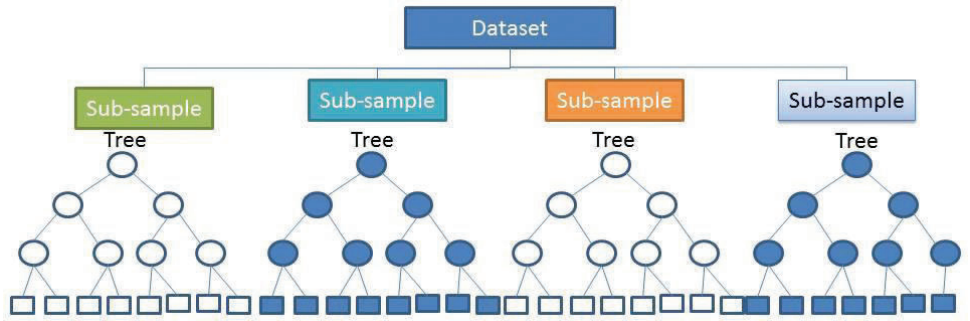
\includegraphics[width=0.8\linewidth]{images/randomForestconcept} 

}

\caption{Schematical representation of data splitting data to generate the random subsets used to train regression trees within a Random forest model (ensemble of regression trees)}\label{fig:rfschema}
\end{figure}

Random forest has been tested by many researchers on digital soil
mapping (see for example \citet{poggio2013regional};
\citet{rad2014updating}, and references therein). For soil carbon
mapping (which for large areas usually rely on sparse datasets), it
holds a lot of promises when compared to other prediction models,
because it's practically free of assumptions. Random Forest has shown
accuracy of spatial predictions and, given the random selection of
subsets and prediction factors, reduce potential over-fitting and data
noise \citep{wiesmeier2011digital}. Over-fitting and data noise are
important uncertainty sources across high dimensionally spaces used to
represent the soil forming environment. Thus, the advent of open-source
platforms and freely downloadable ancillary data (e.g., worldgrids.org)
to represent the soil forming environment makes of random forest and
other such models increasingly appealing on digital soil mapping.

To predict continuous data (such as carbon density) Random forest
generates an averaged ensemble of regression trees based on bagging,
which is the statistical term for the random selection of subsets and
predictors to generate each regression tree. Bagging is a bootstrapping
aggregation technique where each sample is different from the original
data set but resembles it in distribution and variability (Breiman,
1996, 2001). Each tree contributes to weight the statistical
relationship between a dependent variable (e.g.~soil property) and its
prediction factors (e.g., terrain attributes, remote sensing, climate
layers and/or legacy maps). Each tree (generated using a different
subset of available data and random combinations of the prediction
factors) is internally evaluated by an out-of-bag cross validation form
which allows assessing the relative importance of the available
prediction factors. Thus, higher weight is given to the most accurate
trees (which use the most informative prediction factors). The final
prediction of new data is the weighted average of all generated trees.
This method has been used to generate accurate predictions of soil
organic carbon from the plot to the global scale and also in a
country-specific basis (Hengl et al., 2014; Bonfatti et al., 2016; Hengl
et al., 2017; Guevara et al., 2018). Random forest can be implemented
for digital soil mapping using open source code \citep[e.g., the R
package of random forest, see][]{breiman2017cutler} and public sources
of environmental information. The objective of this chapter is to
demonstrate a reproducible framework for the implementation of the
Random forest algorithm applied for soil organic carbon predictive
mapping, including the uncertainty of model estimates and using open
source platforms for statistical computing.

\hypertarget{conceptual-model-and-data-preparation}{%
\subsection{Conceptual model and data
preparation}\label{conceptual-model-and-data-preparation}}

To use Random forest for digital soil organic carbon mapping the SCORPAN
(Soils, Climate, Organisms, Relief, Parent material, Age and N space)
conceptual model (McBratney et al., 2003; Florinsky, 2012) will have
take the following form:
\(\ \text{SOC}_{x,y~t} \sim \text{randomForest} (E_{x,y~t})\) where soil
organic carbon estimates (\emph{SOC}) for a specific site (\emph{x,y})
and for a specific period of time (\textasciitilde{}t) can be modeled as
a Random forest (randomForest) function of the soil forming environment
(\(\ Ex,y~t\)), which is represented by the \emph{SOC} prediction
factors (e.g., terrain attributes, remote sensing, climate layers and/or
legacy maps). To feed the right side of the equation, \(SOC_{x,y~t}\) is
usually represented in a tabular form or a geospatial object (e.g.,
shapefile) with three fundamental columns. Two columns represent the
spatial coordinates x and y (e.g., latitude and longitude) that are used
to extract the values of the prediction factors for the representative
locations of the \emph{SOC} estimates. \emph{SOC} estimates are
represented in a third column (see previous chapters of this book
dealing with the transformation of soil carbon density to mass units).
The left side of the equation is generally represented by gridded
(raster) files, so all available sources of information should be first
harmonized into a common pixel size and coordinate reference system.

\hypertarget{software}{%
\subsection{Software}\label{software}}

For the Random Forest implementation, we will use the platform for
statistical computing R (R Core Team, 2016). This is an open source
object-oriented software that relies on specific-contributor libraries.
There are several libraries for the implementation of the Random forest
algorithm in R as well as several variants of the method that can be
used to solve digital soil mapping problems. In this section, we will
show the use of Random forest using the randomForest, the
quantregForest, the raster and the caret R packages. The quantile
regression forest (quantregForest; (Meinshausen, 2006)) has two main
advantages. First, it can be used to extract the variance of all the
trees generated by Random forest, not just the mean (as in the original
randomForest package), and therefore we can calculate the dispersion of
the full conditional distribution of SOC as a function of the prediction
factors, which given available data, represent the Random forest model
uncertainty. Second, the quantile regression forest approach can also
run in parallel using all available computational resources, in a way
that we can predict and estimate the uncertainty of predictions at
reasonable time frames whit large datasets.

\hypertarget{tunning-random-forest-parameters}{%
\subsection{Tunning Random forest
parameters}\label{tunning-random-forest-parameters}}

Two important parameters of Random forest are mtry and ntree. The mtry
parameter controls the number of prediction factors that are randomly
used on each tree, while the ntree parameter controls the number of
trees generated by Random forest. These two parameters can be selected
by the means of cross-validation to maximize the prediction capacity of
Random forest. We will use the caret package to select the most
appropriate values for these parameters using 10-fold cross-validation
(Kuhn et al.~2017). Tunning the main parameters of Random forest (or any
other model) can be time-consuming in computational terms because
implies the need to run and internally validate an independent model for
each possible combination of parameter values. Thus, tunning the Random
forest parameters would be relevant, given available data, to achieve
the best possible accuracy of predictions.

\hypertarget{technical-steps---random-forest}{%
\subsection{Technical steps - Random
forest}\label{technical-steps---random-forest}}

We will use the Macedonia dataset for this exercise (see previous
chapters of this book dealing with data preparation). The first dataset
contains in a tabular form the \emph{OCSKGM} values and the values of
the prediction factors for the same locations (e.g., x, y,
\emph{OCSKGM}, covariate1, covariate2\ldots{}) while the second database
is represented by a stack of raster files containing prediction factors
across all the area of interest at the spatial resolution of 0.0083º
(approx. 1km). Import the datasets and load in R all our libraries of
interest.

\hypertarget{data-preparation-2}{%
\subsubsection{Data Preparation}\label{data-preparation-2}}

\textbf{Point Dataset}

We previously applied spline function to produce continuous soil
information to a given soil depth (0-30 cm) in section
\ref{EqualAreaSplines}. Spline function basically imports soil profile
data (including instances where layers are not contiguous), fits it to a
mass-preserving spline and outputs attribute means for a given depth.
The output file should contain profile id, upper (surface) and lower
depth (30cm), the estimated value for the selected soil attribute
(Value) and tmse (estimated mean squared error of the spline). If you
used the Spline Tool V2, the coordinates were not kept in the output
file. The coordinates should be added back in the data table. You can
use Profile IDs to add the X, Y columns back. Once your point dataset is
ready, copy this table into your working directory as a .csv file.

\textbf{Environmental Predictors (Covariates)}

In the Chapter \ref{covariates}, we presented and prepared several
global and continental data sets. In addition to these datasets,
numerous covariate layers have been prepared by ISRIC for the GSOC Map
project. These are GIS raster layers of various biophysical earth
surface properties for each country in the world. Some of these layers
will be used as predictors in this section. Please download the
covariates for your own study area from GSOCMap Data Repository as
explained in Section \ref{GSOCDataRepo}.

In section \ref{overlay-soil-covariates}, a table with the points values
after data preparation and the values of our spatial predictors was
prepared. This step involves loading this table.

Now we will import our point dataset using \texttt{read.csv()} function.
The easiest way to create a data frame is to read in data from a
file---this is done using the function read.csv, which works with comma
delimited files. Data can be read in from other file formats as well,
using different functions, but read.csv is the most commonly used
approach. R is very flexible in how it reads in data from text files
(\texttt{read.table}, \texttt{read.csv}, \texttt{read.csv2},
\texttt{read.delim}, \texttt{read.delim2}). Please type
\texttt{?read.table()} for help.

\begin{Shaded}
\begin{Highlighting}[]
\CommentTok{# load data}
\NormalTok{dat <-}\StringTok{ }\KeywordTok{read.csv}\NormalTok{(}\StringTok{"data/MKD_RegMatrix.csv"}\NormalTok{)}

\NormalTok{dat}\OperatorTok{$}\NormalTok{LCEE10 <-}\StringTok{ }\KeywordTok{as.factor}\NormalTok{(dat}\OperatorTok{$}\NormalTok{LCEE10)}
\NormalTok{dat}\OperatorTok{$}\NormalTok{soilmap <-}\StringTok{ }\KeywordTok{as.factor}\NormalTok{(dat}\OperatorTok{$}\NormalTok{soilmap)}

\CommentTok{# explore the data structure}
\KeywordTok{str}\NormalTok{(dat)}
\end{Highlighting}
\end{Shaded}

\begin{verbatim}
## 'data.frame':    2897 obs. of  23 variables:
##  $ id       : Factor w/ 2897 levels "P0003","P0007",..: 1 2 3 4..
##  $ Y        : num  42 42 42.1 42 42 ...
##  $ X        : num  20.8 20.8 20.8 20.9 20.9 ...
##  $ SOC      : num  26.38 6.15 3.94 3.26 2.29 ...
##  $ BLD      : num  0.73 1.17 1.3 1.34 1.41 ...
##  $ CRFVOL   : num  8 18.6 31.9 21.7 14.5 ...
##  $ OCSKGM   : num  5.32 1.75 1.04 1.03 0.83 ...
##  $ meaERROR : num  2.16 2.85 2.65 3.16 3.63 2.83 2.94 2.49 2.77..
##  $ OCSKGMlog: num  1.6712 0.5591 0.0429 0.0286 -0.1862 ...
##  $ B04CHE3  : num  574 553 693 743 744 ...
##  $ B07CHE3  : num  38.5 37.8 42.1 43.7 43.7 ...
##  $ B13CHE3  : num  111.6 125 99.8 118.1 121 ...
##  $ B14CHE3  : num  59.2 60.3 42.4 39.9 38.7 ...
##  $ DEMENV5  : int  2327 2207 1243 1120 1098 1492 1413 1809 1731..
##  $ LCEE10   : Factor w/ 4 levels "1","2","3","4": 1 3 2 1 2 2 2..
##  $ PRSCHE3  : num  998 1053 780 839 844 ...
##  $ SLPMRG5  : int  13 36 6 25 30 24 15 17 20 43 ...
##  $ TMDMOD3  : int  282 280 285 288 289 287 286 286 287 286 ...
##  $ TMNMOD3  : int  272 270 277 279 279 277 277 273 274 273 ...
##  $ TWIMRG5  : int  61 62 81 66 65 72 68 67 65 59 ...
##  $ VBFMRG5  : int  0 0 14 0 0 0 0 0 0 0 ...
##  $ VDPMRG5  : int  311 823 10048 1963 -173 -400 -9 -692 -1139 2..
##  $ soilmap  : Factor w/ 20 levels "1","2","3","4",..: 6 14 14 3..
\end{verbatim}

Since we will be working with spatial data we need to define the
coordinates for the imported data. Using the coordinates() function from
the sp package we can define the columns in the data frame to refer to
spatial coordinates---here the coordinates are listed in columns X and
Y.

\begin{Shaded}
\begin{Highlighting}[]
\KeywordTok{library}\NormalTok{(sp)}

\CommentTok{# Promote to spatialPointsDataFrame}
\KeywordTok{coordinates}\NormalTok{(dat) <-}\StringTok{ }\ErrorTok{~}\StringTok{ }\NormalTok{X }\OperatorTok{+}\StringTok{ }\NormalTok{Y}

\KeywordTok{class}\NormalTok{(dat)}
\end{Highlighting}
\end{Shaded}

\begin{verbatim}
## [1] "SpatialPointsDataFrame"
## attr(,"package")
## [1] "sp"
\end{verbatim}

SpatialPointsDataFrame structure is essentially the same data frame,
except that additional ``spatial'' elements have been added or
partitioned into slots. Some important ones being the bounding box (sort
of like the spatial extent of the data), and the coordinate reference
system proj4string(), which we need to define for the sample dataset. To
define the CRS, we must know where our data are from, and what was the
corresponding CRS used when recording the spatial information in the
field. For this data set, the CRS used was: WGS84 (EPSG:4326).

To clearly tell R this information we define the CRS which describes a
reference system in a way understood by the
\href{http://trac.osgeo.org/proj/}{PROJ.4 projection library}. An
interface to the PROJ.4 library is available in the rgdal package. As a
lternative to using Proj4 character strings, we can use the
corresponding yet simpler EPSG code (European Petroleum Survey Group).
rgdal also recognizes these codes. If you are unsure of the Proj4 or
EPSG code for the spatial data that you have but know the CRS, you
should consult \url{http://spatialreference.org/} for assistance.

Please also note that, when working with spatial data, it's very
important that the CRS (coordinate reference system) of the point data
and covariates are the same.

Now, we will define our CRS:

\begin{Shaded}
\begin{Highlighting}[]
\NormalTok{dat}\OperatorTok{@}\NormalTok{proj4string <-}\StringTok{ }\KeywordTok{CRS}\NormalTok{(}\DataTypeTok{projargs =} \StringTok{"+init=epsg:4326"}\NormalTok{)}

\NormalTok{dat}\OperatorTok{@}\NormalTok{proj4string}
\end{Highlighting}
\end{Shaded}

\begin{verbatim}
## CRS arguments:
##  +init=epsg:4326 +proj=longlat +datum=WGS84 +no_defs
## +ellps=WGS84 +towgs84=0,0,0
\end{verbatim}

Now we will import the covariates. When the covariate layers are in
common resolution and extent, rather than working with individual
rasters it is better to stack them all into a single R object. In this
example, we use 13 covariates from the GSOCMap Data Repository and a
rasterized version of the soil type map. The rasterization of vectorial
data was covered in
\protect\hyperlink{technical-steps---rasterizing-a-vector-layer-in-r}{Technical
Steps - Rasterizing a vector layer in R}. The file containing all the
covariates was prepared at the end of chapter \ref{covariates}.

\begin{Shaded}
\begin{Highlighting}[]
\KeywordTok{load}\NormalTok{(}\DataTypeTok{file =} \StringTok{"covariates.RData"}\NormalTok{)}

\KeywordTok{names}\NormalTok{(covs)}
\end{Highlighting}
\end{Shaded}

\begin{verbatim}
##  [1] "B04CHE3" "B07CHE3" "B13CHE3" "B14CHE3" "DEMENV5" "LCEE10" 
##  [7] "PRSCHE3" "SLPMRG5" "TMDMOD3" "TMNMOD3" "TWIMRG5" "VBFMRG5"
## [13] "VDPMRG5" "soilmap"
\end{verbatim}

Random forest does not have assumptions about the statistical
distribution of the response variable, but it is a good practice prior
to model building to analyze the statistical distribution of the
response variable (e.g., if is normal or not) and its relationships with
the prediction factors. Soil organic carbon tends to have a log-normal
distribution with a right-skew, and transforming the original values to
its natural logarithm would generate a normal distribution of soil
organic carbon values. For further analysis, we will use the dataset
transformed to its natural logarithm (OCSKGMlog) because this
transformation, given this dataset, increases the correlation of the
response variable and the covariate space.

Keep in mind that selecting the most appropriate prediction factors is
required to generate an interpretable model and high accuracy of
prediction in places where no information is available. Variable
selection ideally should incorporate expert soil knowledge about the
study area and statistical criteria (e.g., just to use the
best-correlated predictors). Multivariate analysis (e.g., principal
component analysis) is a widely used approach to identify informative
predictors. Here we use this combination of prediction factors to be
consistent with other book chapters and because they were previously
selected for this exercise using expert knowledge about the spatial
variability of soil organic carbon. Now, we will build a working
hypothesis from our conceptual model, using all the continuous
prediction factors for \emph{OCSKGMlog}:

\emph{OCSKGMlog} \textasciitilde{} randomForest \emph{B04CHE3 + B07CHE3
+ B13CHE3 + B14CHE3 + DEMENV5 + LCEE10 + PRSCHE3 + SLPMRG5 + TMDMOD3 +
TMNMOD3 + TWIMRG5 + VBFMRG5 + VDPMRG5}

\begin{Shaded}
\begin{Highlighting}[]
\CommentTok{# For its use on R we need to define a model formula}

\NormalTok{fm =}\StringTok{ }\KeywordTok{as.formula}\NormalTok{(}\KeywordTok{paste}\NormalTok{(}\StringTok{"log(OCSKGM) ~"}\NormalTok{, }\KeywordTok{paste0}\NormalTok{(}\KeywordTok{names}\NormalTok{(covs[[}\OperatorTok{-}\DecValTok{14}\NormalTok{]]),}
                                            \DataTypeTok{collapse =} \StringTok{"+"}\NormalTok{))) }
\end{Highlighting}
\end{Shaded}

This is the R syntax to define a model formula required for the model
structure, where soil organic carbon transformed to its natural
logarithm (\emph{OCSKGMlog}) can be predicted as a function of the
available prediction factors (each explained in previous chapters of
this book, e.g., B04CHE3, B07CHE3, B13CHE3, B14CHE3, DEMENV5 , LCEE10,
PRSCHE3, SLPMRG5, TMDMOD3, TMNMOD3, TWIMRG5, VBFMRG5, VDPMRG5).

Note that the variable soilmap is categorical, so is not included in the
correlation analysis. In fact, although soil type polygon maps are in
theory powerful predictors for \emph{OCSKGM} we will not use this map
for this exercise, because not all categories in the map are represented
by available \emph{OCSKGM} estimates, therefore this map requires a
generalization of soil type units in function of the classes represented
by the sites of \emph{OCSKGM} estimates, which is beyond the scope of
this chapter. Ideally, the number of observations across all the
categories of soil type or any other factorial variable should be
balanced. Another alternative to using an unbalanced categorical map is
by generating dummy variables, where each category in the map becomes an
independent binomial predictor variable (e.g., only 0 and 1 values) as
is explained in the following chapter. The risk of doing so rely upon
the potential underestimation of the spatial variability of the target
variable under each category with a low density of available data.

\hypertarget{tuning-parameters}{%
\subsubsection{Tuning parameters}\label{tuning-parameters}}

Now we will use the cross-validation strategy implemented in the train
function of the caret package (Kuhn et al.~2017), which default is
10-fold. The result of this function includes information to select the
best mtry parameter and to decide the appropriate number of trees. The
out-of-bag root mean squared error (rmse) will be used to select the
optimal mtry model. To analyze the ntree parameter we will plot the
number of trees against the out-of-bag rmse, an optimal ntree can be
selected with the number of trees when these relationships stabilizes at
the minimum possible rmse (in the y axis). Reduncing the number of trees
will reduce the computational demand, which is specially important when
dealing with large databases. In the presence of multidimensional and
highly correlated prediction factors, avoiding an excessive number of
trees will also reduce the risk of model overfitting.

\begin{Shaded}
\begin{Highlighting}[]
\KeywordTok{library}\NormalTok{(randomForest)}
\KeywordTok{library}\NormalTok{(caret)}

\CommentTok{# Default 10-fold cross-validation}
\NormalTok{ctrl <-}\StringTok{ }\KeywordTok{trainControl}\NormalTok{(}\DataTypeTok{method =} \StringTok{"cv"}\NormalTok{, }\DataTypeTok{savePred=}\NormalTok{T)}
\CommentTok{# Search for the best mtry parameter}
\NormalTok{rfmodel <-}\StringTok{ }\KeywordTok{train}\NormalTok{(fm, }\DataTypeTok{data=}\NormalTok{dat}\OperatorTok{@}\NormalTok{data, }\DataTypeTok{method =} \StringTok{"rf"}\NormalTok{, }\DataTypeTok{trControl =}\NormalTok{ ctrl, }
             \DataTypeTok{importance=}\OtherTok{TRUE}\NormalTok{)}
\CommentTok{# This is a very useful function to compare and test different }
\CommentTok{# prediction algorithms. Type names(getModelInfo()) to see all the }
\CommentTok{# possibilitites implemented on this function}
\end{Highlighting}
\end{Shaded}

The object derived from the train function can be used to generate
predictions of OCSKGMlog at the spatial resolution of the prediction
factors. Before generating predictions, we will plot the most important
predictors sorted in decreasing order of importance. From the variable
importance plot, \%IncMSE represent an informative measure for variable
selection. It is the increase in error (mean squared error, MSE) of
predictions which was estimated with out-of-bag-cross validation as a
result of prediction factor being permuted with values randomly
shuffled. This is one of the strategies that Random forest uses to
reduce overfitting.

\begin{Shaded}
\begin{Highlighting}[]
\CommentTok{# Variable importance plot, compare with the correlation matrix}
\CommentTok{# Select the best prediction factors and repeat  }
\KeywordTok{varImpPlot}\NormalTok{(rfmodel[}\DecValTok{11}\NormalTok{][[}\DecValTok{1}\NormalTok{]])}
\end{Highlighting}
\end{Shaded}

\begin{figure}
\centering
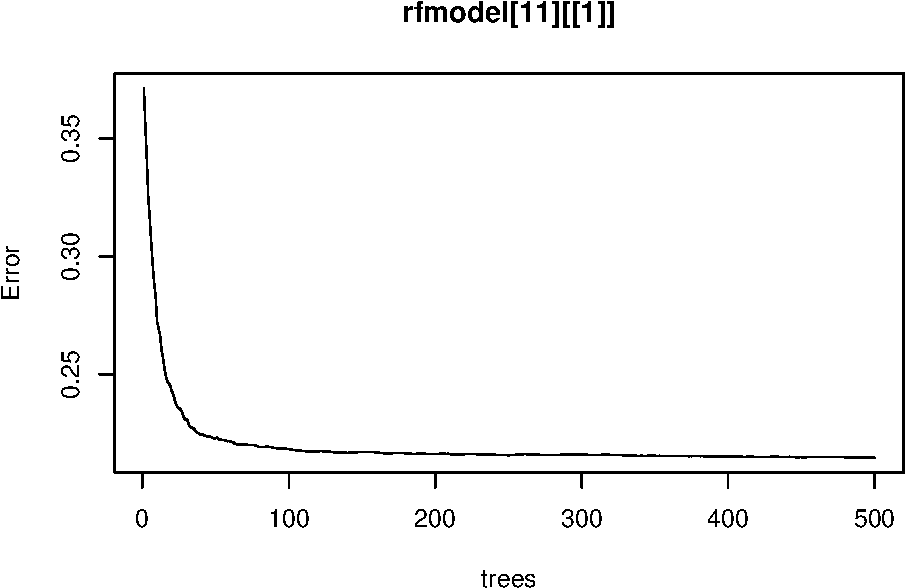
\includegraphics{SOCMapping_files/figure-latex/unnamed-chunk-60-1.pdf}
\caption{\label{fig:unnamed-chunk-60}Model Decreasing Error and Node Purity}
\end{figure}

\begin{Shaded}
\begin{Highlighting}[]
\CommentTok{# Check if the error stabilizes }
\KeywordTok{plot}\NormalTok{(rfmodel[}\DecValTok{11}\NormalTok{][[}\DecValTok{1}\NormalTok{]])}
\end{Highlighting}
\end{Shaded}

\begin{figure}
\centering
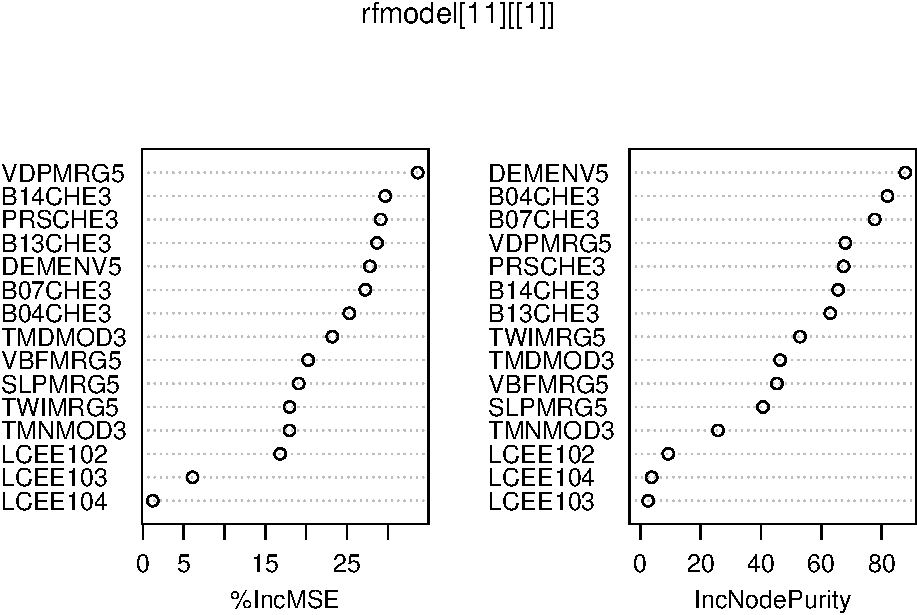
\includegraphics{SOCMapping_files/figure-latex/unnamed-chunk-61-1.pdf}
\caption{\label{fig:unnamed-chunk-61}select ntree}
\end{figure}

Random forest users are encouraged to compare and test the prediction
capacity of different combinations of prediction factors in order to
reduce the complexity of the model and the statistical redundancy of
environmental information on further applications of predicted OCSKGM
maps (e.g., quantifying the carbon dynamics). The resulting map of our
Random forest model needs to be validated using the independent dataset
to complement the results of the cross-validation (e.g., rmse and
explained variance) derived using the train function and to have a more
comprehensive interpretation of accuracy and bias. Note how the rmse and
the explained variance derived from the independent validations are
slightly lower than the values obtained using cross-validation.

\begin{Shaded}
\begin{Highlighting}[]
\CommentTok{#Make a prediction across all Macedonia}
\CommentTok{#Note that the units are still in log}
\NormalTok{pred <-}\StringTok{ }\KeywordTok{predict}\NormalTok{(covs, rfmodel)}
\end{Highlighting}
\end{Shaded}

\begin{verbatim}
## Warning in .local(object, ...): not sure if the correct factor
## levels are used here
\end{verbatim}

\begin{Shaded}
\begin{Highlighting}[]
\CommentTok{# Back transform predictions log transformed}
\NormalTok{pred <-}\StringTok{ }\KeywordTok{exp}\NormalTok{(pred)}

\CommentTok{# Save the result as a tiff file}
\KeywordTok{writeRaster}\NormalTok{(pred, }\DataTypeTok{filename =} \StringTok{"results/MKD_OCSKGM_rf.tif"}\NormalTok{,}
            \DataTypeTok{overwrite=}\OtherTok{TRUE}\NormalTok{)}


\KeywordTok{plot}\NormalTok{(pred)}
\end{Highlighting}
\end{Shaded}

\begin{figure}
\centering
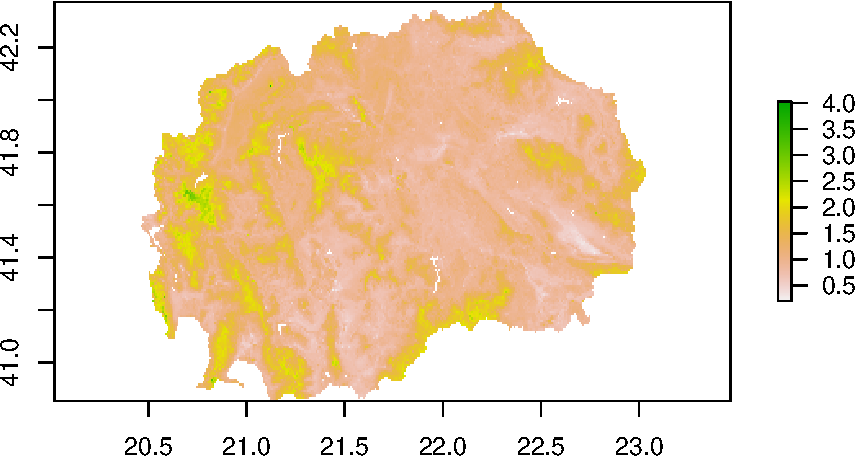
\includegraphics{SOCMapping_files/figure-latex/rf-pred-1.pdf}
\caption{\label{fig:rf-pred}SOC prediction using a randomForest model}
\end{figure}

\hypertarget{modelling-uncertainty-using-random-forest}{%
\subsection{Modelling Uncertainty Using Random
Forest}\label{modelling-uncertainty-using-random-forest}}

Ideally, a digital soil map should include a spatial explicit metric of
uncertainty. The uncertainty can be roughly divided into four main
components, uncertainty in soil data, uncertainty in soil covariates,
uncertainty in the model and uncertainty in variations of available
data. Here, we show an approach to estimate the sensitivity of the model
to available data and the uncertainty of the model. The first two are
beyond of the aim of this chapter. For the third and fourth we will
generate a reproducible example.

\hypertarget{technical-steps---using-quantile-regression-forest-to-estimate-uncertainty}{%
\subsubsection{Technical steps - Using Quantile Regression Forest to
estimate
uncertainty}\label{technical-steps---using-quantile-regression-forest-to-estimate-uncertainty}}

To analyze the sensitivity of the model to available data we need to
randomly split the data several times (e.g., 10 or more, is possible
until the variance stabilizes) in training and testing subsets. A model
generation and prediction are made on each split, in a way that the
dispersion of the predicted values at the pixel level will represent the
uncertainty and the sensitivity of the model to variations in available
data. This process increases computational demand and memory since it
will repeat n times (10 in this example) the model and the prediction
using each time a different random combination of data for training and
testing the models. As larger the sample and the number of realizations
the more robust our validation strategy. For this example, we will use
only 10 realizations and random splits of 25\% of available data. The
validation plot shows the regression line between observed and predicted
of a model that uses 75\% (black line) and the regression lines of 10
model realizations, each with a different random combination of data for
training and validating the models. The rmse and the explained variance
of the models is stored in the object validation (type
\texttt{summary(validation)}). The standard deviation of all the ten
predictions allows generating a map of model sensitivity to available
data.

\begin{Shaded}
\begin{Highlighting}[]
\CommentTok{#Generate an empty dataframe}
\NormalTok{validation <-}\StringTok{ }\KeywordTok{data.frame}\NormalTok{(}\DataTypeTok{rmse=}\KeywordTok{numeric}\NormalTok{(), }\DataTypeTok{r2=}\KeywordTok{numeric}\NormalTok{())}
\CommentTok{#Sensitivity to the dataset}
\CommentTok{#Start a loop with 10 model realizations}
\ControlFlowTok{for}\NormalTok{ (i }\ControlFlowTok{in} \DecValTok{1}\OperatorTok{:}\DecValTok{10}\NormalTok{)\{}
  \CommentTok{# We will build 10 models using random samples of 25%  }
\NormalTok{  smp_size <-}\StringTok{ }\KeywordTok{floor}\NormalTok{(}\FloatTok{0.25} \OperatorTok{*}\StringTok{ }\KeywordTok{nrow}\NormalTok{(dat))}
\NormalTok{  train_ind <-}\StringTok{ }\KeywordTok{sample}\NormalTok{(}\KeywordTok{seq_len}\NormalTok{(}\KeywordTok{nrow}\NormalTok{(dat)), }\DataTypeTok{size =}\NormalTok{ smp_size)}
\NormalTok{  train <-}\StringTok{ }\NormalTok{dat[train_ind, ]}
\NormalTok{  test <-}\StringTok{ }\NormalTok{dat[}\OperatorTok{-}\NormalTok{train_ind, ]}
\NormalTok{  modn <-}\StringTok{ }\KeywordTok{train}\NormalTok{(fm, }\DataTypeTok{data=}\NormalTok{train, }\DataTypeTok{method =} \StringTok{"rf"}\NormalTok{, }\DataTypeTok{trControl =}\NormalTok{ ctrl)}
\NormalTok{  pred <-}\StringTok{ }\KeywordTok{stack}\NormalTok{(pred, }\KeywordTok{predict}\NormalTok{(covariates, modn))}
\NormalTok{  test}\OperatorTok{$}\NormalTok{pred <-}\StringTok{ }\KeywordTok{predict}\NormalTok{(modn[}\DecValTok{11}\NormalTok{][[}\DecValTok{1}\NormalTok{]], test)}
  \CommentTok{# Store the results in a dataframe}
\NormalTok{  validation[i, }\DecValTok{1}\NormalTok{] <-}\StringTok{ }\KeywordTok{rmse}\NormalTok{(test}\OperatorTok{$}\NormalTok{OCSKGMlog, test}\OperatorTok{$}\NormalTok{pred)}
\NormalTok{  validation[i, }\DecValTok{2}\NormalTok{] <-}\StringTok{ }\KeywordTok{cor}\NormalTok{(test}\OperatorTok{$}\NormalTok{OCSKGMlog, test}\OperatorTok{$}\NormalTok{pred)}\OperatorTok{^}\DecValTok{2}
\NormalTok{\}}
\end{Highlighting}
\end{Shaded}

\begin{Shaded}
\begin{Highlighting}[]
\CommentTok{#The sensitivity map is the dispersion of all individual models}
\NormalTok{sensitivity <-}\StringTok{ }\KeywordTok{calc}\NormalTok{(pred[[}\OperatorTok{-}\DecValTok{1}\NormalTok{]], sd)}

\KeywordTok{plot}\NormalTok{(sensitivity, }\DataTypeTok{col=}\KeywordTok{rev}\NormalTok{(}\KeywordTok{topo.colors}\NormalTok{(}\DecValTok{10}\NormalTok{)), }
     \DataTypeTok{main=}\StringTok{'Sensitivity based on 10 realizations using 25% samples'}\NormalTok{)}
\end{Highlighting}
\end{Shaded}

\begin{Shaded}
\begin{Highlighting}[]
\CommentTok{#Sensitivity of validation metrics}
\KeywordTok{summary}\NormalTok{(validation)}
\end{Highlighting}
\end{Shaded}

\begin{Shaded}
\begin{Highlighting}[]
\CommentTok{# Plot of the map based on 75% of data and the sensitivity to data }
\CommentTok{# variations}
\NormalTok{prediction75 <-}\StringTok{ }\KeywordTok{exp}\NormalTok{(pred[[}\DecValTok{1}\NormalTok{]])}

\KeywordTok{plot}\NormalTok{(prediction75, }\DataTypeTok{main=}\StringTok{'OCSKGM prediction based on 75% of data'}\NormalTok{, }
     \DataTypeTok{col=}\KeywordTok{rev}\NormalTok{(}\KeywordTok{topo.colors}\NormalTok{(}\DecValTok{10}\NormalTok{)))}
\end{Highlighting}
\end{Shaded}

Finally, we will estimate the model uncertainty, represented by the full
conditional distribution of the response variable (OCSKGMlog) as a
function of the selected prediction factors using the quantile
regression forest package of R. This approach has proven to be efficient
for digital soil mapping across large areas \citep{vaysse2017using}.

\begin{Shaded}
\begin{Highlighting}[]
\CommentTok{# Use quantile regression forest to estimate the full conditional }
\CommentTok{# distribution of OCSKGMlog, note that we are using the mtry }
\CommentTok{# parameter that was selected by the train function of the caret }
\CommentTok{# package, assuming that the 75% of data previously used well }
\CommentTok{# resembles the statistical distribution of the entire data }
\CommentTok{# population. Otherwise, repeat the train function with all available }
\CommentTok{# data (using the object dat that instead of train) to select mtry.}


\NormalTok{model <-}\StringTok{ }\KeywordTok{quantregForest}\NormalTok{(}\DataTypeTok{y=}\NormalTok{dat}\OperatorTok{$}\NormalTok{OCSKGMlog, }\DataTypeTok{x=}\NormalTok{dat[,}\DecValTok{1}\OperatorTok{:}\DecValTok{13}\NormalTok{], }\DataTypeTok{ntree=}\DecValTok{500}\NormalTok{, }
                   \DataTypeTok{keep.inbag=}\OtherTok{TRUE}\NormalTok{, }\DataTypeTok{mtry =} \KeywordTok{as.numeric}\NormalTok{(mod}\OperatorTok{$}\NormalTok{bestTune))                        }
\end{Highlighting}
\end{Shaded}

This method will calculate a probability distribution function for each
pixel and therefore can be time-consuming. Therefore we will run it
using parallel computing. Note that the code to run in parallel this
analysis can also be passed to the previous predictions (predict
function). The result will be a map of the standard deviation of the
distribution calculated for each pixel, which represents the extreme
values that a prediction can take for a specific site (e.g., pixel)
given available data and predictors. Note that this analysis is
performed using all available data and a second map of OCSKGM is
created. Our final prediction uses all available data, while the total
uncertainty (in percent) is represented by the sum of the quantile
regression forest standard deviation and the sensitivity map from the
previous section. The total uncertainty is then divided by the
prediction to obtain a percent map, which is easier to interpret.

\begin{Shaded}
\begin{Highlighting}[]
\KeywordTok{library}\NormalTok{(snow)}
\CommentTok{# Estimate model uncertainty at the pixel level using parallel }
\CommentTok{# computing}
\KeywordTok{beginCluster}\NormalTok{() }\CommentTok{#define number of cores to use}
\CommentTok{# Estimate model uncertainty}
\NormalTok{unc <-}\StringTok{ }\KeywordTok{clusterR}\NormalTok{(covariates, predict, }\DataTypeTok{args=}\KeywordTok{list}\NormalTok{(}\DataTypeTok{model=}\NormalTok{model,}\DataTypeTok{what=}\NormalTok{sd))}
\CommentTok{# OCSKGMlog prediction based in all available data}
\NormalTok{mean <-}\StringTok{ }\KeywordTok{clusterR}\NormalTok{(covariates, predict, }
                 \DataTypeTok{args=}\KeywordTok{list}\NormalTok{(}\DataTypeTok{model=}\NormalTok{model, }\DataTypeTok{what=}\NormalTok{mean))}
\CommentTok{# The total uncertainty is the sum of sensitivity and model }
\CommentTok{# uncertainty}
\NormalTok{unc <-}\StringTok{ }\NormalTok{unc }\OperatorTok{+}\StringTok{ }\NormalTok{sensitivity}
\CommentTok{# Express the uncertainty in percent (divide by the mean)}
\NormalTok{Total_unc_Percent <-}\StringTok{ }\KeywordTok{exp}\NormalTok{(unc)}\OperatorTok{/}\KeywordTok{exp}\NormalTok{(mean)}
\KeywordTok{endCluster}\NormalTok{()}
\end{Highlighting}
\end{Shaded}

\begin{Shaded}
\begin{Highlighting}[]
\CommentTok{# Plot both maps (the predicted OCSKGM + its associated uncertainty)}
\KeywordTok{plot}\NormalTok{(}\KeywordTok{exp}\NormalTok{(mean), }\DataTypeTok{main=}\StringTok{'OCSKGM based in all data'}\NormalTok{, }
     \DataTypeTok{col=}\KeywordTok{rev}\NormalTok{(}\KeywordTok{topo.colors}\NormalTok{(}\DecValTok{10}\NormalTok{)))}
\end{Highlighting}
\end{Shaded}

\begin{Shaded}
\begin{Highlighting}[]
\KeywordTok{plot}\NormalTok{(Total_unc_Percent, }\DataTypeTok{col=}\KeywordTok{rev}\NormalTok{(}\KeywordTok{heat.colors}\NormalTok{(}\DecValTok{100}\NormalTok{)), }\DataTypeTok{zlim=}\KeywordTok{c}\NormalTok{(}\DecValTok{0}\NormalTok{, }\DecValTok{5}\NormalTok{), }
     \DataTypeTok{main=}\StringTok{'Total uncertainty'}\NormalTok{)}
\end{Highlighting}
\end{Shaded}

Finally, the predicted OCSKGM and the total uncertainty can be saved in
the working directory in a generic (*.tif) raster format.

\begin{Shaded}
\begin{Highlighting}[]
\CommentTok{#Save the resulting maps in separated *.tif files}
\KeywordTok{writeRaster}\NormalTok{(}\KeywordTok{exp}\NormalTok{(mean), }\DataTypeTok{file=}\StringTok{'rfOCSKGMprediction.tif'}\NormalTok{, }
            \DataTypeTok{overwrite=}\OtherTok{TRUE}\NormalTok{)}
\KeywordTok{writeRaster}\NormalTok{(Total_unc_Percent, }\DataTypeTok{file=}\StringTok{'rfOCSKGMtotalUncertPercent.tif'}\NormalTok{,}
            \DataTypeTok{overwrite=}\OtherTok{TRUE}\NormalTok{)}
\end{Highlighting}
\end{Shaded}

We have created two maps in the working directory, one represents the
predicted OCSKGM and the second one its uncertainty, which is the sum of
the model sensitivity to data variations and the full conditional
distribution of the response variable as a function of available
prediction factors. The following chapters of this book will show you
how to prepare a stock report based on this soil carbon digital soil
maps.

\clearpage

\hypertarget{svm}{%
\section{Data mining: Support Vector Machines}\label{svm}}

\emph{GF Olmedo \& M Guevara}

\hypertarget{overview-3}{%
\subsection{Overview}\label{overview-3}}

Support vector machines (svm) is a kernel-based machine learning
technique suitable for mapping SOC. svm use decision surfaces (defined
by a kernel function) to map non-linear relationships across a
high-dimension induced feature space (Cortes and Vapnik 1995, Machine
Learning,20, 273-297). svm is widely used to perform classification and
regression analysis on digital soil mapping. According to \citet{scikit}
the advantages of svm are:

\begin{itemize}
\tightlist
\item
  Effective in high dimensional spaces.
\item
  Still effective in cases where the number of dimensions is greater
  than the number of samples.
\item
  Uses a subset of training points in the decision function (called
  support vectors), so it is also memory efficient.
\item
  Versatile: different Kernel functions can be specified for the
  decision function. Common kernels are provided, but it is also
  possible to specify custom kernels.
\end{itemize}

And the disadvantages of svm include:

\begin{itemize}
\tightlist
\item
  If the number of features is much greater than the number of samples,
  avoid over-fitting in choosing Kernel functions and regularization
  term is crucial.
\item
  svm do not directly provide probability estimates, these are
  calculated using an expensive five-fold cross-validation.
\end{itemize}

In digital soil mapping, the problems usually involve working in high
dimensional spaces (were the dimensions are the covariates) with a
limited number of samples. svm is a technique mostly used in
classification problems, but it can be used to solve regression
problems, such as modeling the continuous variability of SOC using
environmental covariates. When svm is used to solve regression problem
is called support vector regression.

Support vector regression applies a simple linear method to the data but
in a high-dimensional feature space non-linearly related to the input
space. It creates n hyperplanes through the n-dimensional spectral-space
and each hyperplanes separates numerical data based on a kernel function
(e.g., Gaussian). svm uses parameters such as gamma, cost and epsilon.
These parameters are used to define the shape of the hyperplane,
including the margin from the closest point to the hyperplane that
divides data with the largest possible margin and defines the tolerance
to errors on each single training. Linear models are fitted to the
support vectors and used for prediction purposes. The support vectors
are the points which fall within each hyperplane \citep{soil-2017-40}.

In the example below, we will use the implementation of svm in the R
package \texttt{e1071} \citep{e1071}. The package e1071 offers an
interface to the award-winning C++ implementation by Chih-Chung Chang
and Chih-Jen Lin, libsvm (current version: 2.6). For further
implementation details on libsvm, see \citet{chang2001libsvm}.

svm is a broad research area and for a better understanding of the
mathematical background we can recommend the following books:
\citet{vapnik2013nature}, \citet{friedman2001elements}, and
\citet{james2013introduction}.

\hypertarget{technical-steps---fitting-an-svm-model-to-predict-the-soc}{%
\subsection{Technical Steps - Fitting an SVM Model to Predict the
SOC}\label{technical-steps---fitting-an-svm-model-to-predict-the-soc}}

\hypertarget{setting-working-space-and-initial-steps-1}{%
\subsubsection{Setting Working Space and Initial
Steps}\label{setting-working-space-and-initial-steps-1}}

One of the first steps should be setting our working directory. If you
read/write files from/ to disk, this takes place in the working
directory. If we don't set the working directory we could easily write
files to an undesirable file location. The following example shows how
to set the working directory in R to our folder which contains data for
the study area (point data, covariates).

Note that we must use the forward slash / or double backslash
\textbackslash{}\textbackslash{} in R! Single backslash \textbackslash{}
will not work. Now we can check if the working directory has been
correctly set by using the function:

\begin{Shaded}
\begin{Highlighting}[]
\KeywordTok{getwd}\NormalTok{()}
\end{Highlighting}
\end{Shaded}

\hypertarget{data-preparation-3}{%
\subsubsection{Data Preparation}\label{data-preparation-3}}

\textbf{Point Dataset}

We previously applied spline function to produce continuous soil
information to a given soil depth (0-30 cm) in the section
\ref{EqualAreaSplines}. Spline function basically imports soil profile
data (including instances where layers are not contiguous), fits it to a
mass-preserving spline and outputs attribute means for a given depth.
The output file should contain profile id, upper (surface) and lower
depth (30cm), estimated value for the selected soil attribute (Value)
and tmse (estimated mean squared error of the spline). If you used the
Spline Tool V2, the coordinates were not kept in the output file. The
coordinates should be added back in the data table. You can use Profile
IDs to add the X, Y columns back. Once your point dataset is ready, copy
this table into your working directory as a .csv file.

\textbf{Environmental Predictors (Covariates)}

In the Chapter \ref{covariates}, we presented and prepared several
global and continental datasets. In addition to these datasets, numerous
covariate layers have been prepared by ISRIC for the GSOC Map project.
These are GIS raster layers of various biophysical earth surface
properties for each country in the world. Some of these layers will be
used as predictors in this section. Please download the covariates for
your own study area from GSOCMap Data Repository as explained in Section
\ref{GSOCDataRepo}.

In section \ref{overlay-soil-covariates}, a table with the points values
after data preparation and the values of our spatial predictors was
prepared. This step involves loading this table.

Now we will import our point dataset using \texttt{read.csv()} function.
The easiest way to create a data frame is to read in data from a
file---this is done using the function read.csv, which works with comma
delimited files. Data can be read in from other file formats as well,
using different functions, but read.csv is the most commonly used
approach. R is very flexible in how it reads in data from text files
(\texttt{read.table}, \texttt{read.csv}, \texttt{read.csv2},
\texttt{read.delim}, \texttt{read.delim2}). Please type
\texttt{?read.table()} for help.

\begin{Shaded}
\begin{Highlighting}[]
\CommentTok{# load data}
\NormalTok{dat <-}\StringTok{ }\KeywordTok{read.csv}\NormalTok{(}\StringTok{"data/MKD_RegMatrix.csv"}\NormalTok{)}

\NormalTok{dat}\OperatorTok{$}\NormalTok{LCEE10 <-}\StringTok{ }\KeywordTok{as.factor}\NormalTok{(dat}\OperatorTok{$}\NormalTok{LCEE10)}
\NormalTok{dat}\OperatorTok{$}\NormalTok{soilmap <-}\StringTok{ }\KeywordTok{as.factor}\NormalTok{(dat}\OperatorTok{$}\NormalTok{soilmap)}

\CommentTok{# explore the data structure}
\KeywordTok{str}\NormalTok{(dat)}
\end{Highlighting}
\end{Shaded}

\begin{verbatim}
## 'data.frame':    2897 obs. of  23 variables:
##  $ id       : Factor w/ 2897 levels "P0003","P0007",..: 1 2 3 4..
##  $ Y        : num  42 42 42.1 42 42 ...
##  $ X        : num  20.8 20.8 20.8 20.9 20.9 ...
##  $ SOC      : num  26.38 6.15 3.94 3.26 2.29 ...
##  $ BLD      : num  0.73 1.17 1.3 1.34 1.41 ...
##  $ CRFVOL   : num  8 18.6 31.9 21.7 14.5 ...
##  $ OCSKGM   : num  5.32 1.75 1.04 1.03 0.83 ...
##  $ meaERROR : num  2.16 2.85 2.65 3.16 3.63 2.83 2.94 2.49 2.77..
##  $ OCSKGMlog: num  1.6712 0.5591 0.0429 0.0286 -0.1862 ...
##  $ B04CHE3  : num  574 553 693 743 744 ...
##  $ B07CHE3  : num  38.5 37.8 42.1 43.7 43.7 ...
##  $ B13CHE3  : num  111.6 125 99.8 118.1 121 ...
##  $ B14CHE3  : num  59.2 60.3 42.4 39.9 38.7 ...
##  $ DEMENV5  : int  2327 2207 1243 1120 1098 1492 1413 1809 1731..
##  $ LCEE10   : Factor w/ 4 levels "1","2","3","4": 1 3 2 1 2 2 2..
##  $ PRSCHE3  : num  998 1053 780 839 844 ...
##  $ SLPMRG5  : int  13 36 6 25 30 24 15 17 20 43 ...
##  $ TMDMOD3  : int  282 280 285 288 289 287 286 286 287 286 ...
##  $ TMNMOD3  : int  272 270 277 279 279 277 277 273 274 273 ...
##  $ TWIMRG5  : int  61 62 81 66 65 72 68 67 65 59 ...
##  $ VBFMRG5  : int  0 0 14 0 0 0 0 0 0 0 ...
##  $ VDPMRG5  : int  311 823 10048 1963 -173 -400 -9 -692 -1139 2..
##  $ soilmap  : Factor w/ 20 levels "1","2","3","4",..: 6 14 14 3..
\end{verbatim}

Since we will be working with spatial data we need to define the
coordinates for the imported data. Using the coordinates() function from
the sp package we can define the columns in the data frame to refer to
spatial coordinates---here the coordinates are listed in columns X and
Y.

\begin{Shaded}
\begin{Highlighting}[]
\KeywordTok{library}\NormalTok{(sp)}

\CommentTok{# Promote to spatialPointsDataFrame}
\KeywordTok{coordinates}\NormalTok{(dat) <-}\StringTok{ }\ErrorTok{~}\StringTok{ }\NormalTok{X }\OperatorTok{+}\StringTok{ }\NormalTok{Y}

\KeywordTok{class}\NormalTok{(dat)}
\end{Highlighting}
\end{Shaded}

\begin{verbatim}
## [1] "SpatialPointsDataFrame"
## attr(,"package")
## [1] "sp"
\end{verbatim}

SpatialPointsDataFrame structure is essentially the same data frame,
except that additional ``spatial'' elements have been added or
partitioned into slots. Some important ones being the bounding box (sort
of like the spatial extent of the data), and the coordinate reference
system proj4string(), which we need to define for the sample dataset. To
define the CRS, we must know where our data are from, and what was the
corresponding CRS used when recording the spatial information in the
field. For this data set, the CRS used was: WGS84 (EPSG:4326).

To clearly tell R this information we define the CRS which describes a
reference system in a way understood by the
\href{http://trac.osgeo.org/proj/}{PROJ.4 projection library}. An
interface to the PROJ.4 library is available in the rgdal package. As an
alternative to using Proj4 character strings, we can use the
corresponding yet simpler EPSG code (European Petroleum Survey Group).
rgdal also recognizes these codes. If you are unsure of the Proj4 or
EPSG code for the spatial data that you have but know the CRS, you
should consult \url{http://spatialreference.org/} for assistance.

Please also note that, when working with spatial data, it's very
important that the CRS (coordinate reference system) of the point data
and covariates are the same.

Now, we will define our CRS:

\begin{Shaded}
\begin{Highlighting}[]
\NormalTok{dat}\OperatorTok{@}\NormalTok{proj4string <-}\StringTok{ }\KeywordTok{CRS}\NormalTok{(}\DataTypeTok{projargs =} \StringTok{"+init=epsg:4326"}\NormalTok{)}

\NormalTok{dat}\OperatorTok{@}\NormalTok{proj4string}
\end{Highlighting}
\end{Shaded}

\begin{verbatim}
## CRS arguments:
##  +init=epsg:4326 +proj=longlat +datum=WGS84 +no_defs
## +ellps=WGS84 +towgs84=0,0,0
\end{verbatim}

Now we will import the covariates. When the covariate layers are in
common resolution and extent, rather than working with individual
rasters it is better to stack them all into a single R object. In this
example, we use 13 covariates from the GSOCMap Data Repository and a
rasterized version of the soil type map. The rasterization of vectorial
data was covered in
\protect\hyperlink{technical-steps---rasterizing-a-vector-layer-in-r}{Technical
Steps - Rasterizing a vector layer in R}. The file containing all the
covariates was prepared at the end of chapter \ref{covariates}.

\begin{Shaded}
\begin{Highlighting}[]
\KeywordTok{load}\NormalTok{(}\DataTypeTok{file =} \StringTok{"covariates.RData"}\NormalTok{)}

\KeywordTok{names}\NormalTok{(covs)}
\end{Highlighting}
\end{Shaded}

\begin{verbatim}
##  [1] "B04CHE3" "B07CHE3" "B13CHE3" "B14CHE3" "DEMENV5" "LCEE10" 
##  [7] "PRSCHE3" "SLPMRG5" "TMDMOD3" "TMNMOD3" "TWIMRG5" "VBFMRG5"
## [13] "VDPMRG5" "soilmap"
\end{verbatim}

\hypertarget{variable-selection-using-correlation-analysis}{%
\subsubsection{Variable selection using correlation
analysis}\label{variable-selection-using-correlation-analysis}}

\begin{Shaded}
\begin{Highlighting}[]
\CommentTok{# plot the names of the covariates}
\KeywordTok{names}\NormalTok{(dat}\OperatorTok{@}\NormalTok{data)}
\end{Highlighting}
\end{Shaded}

\begin{verbatim}
##  [1] "id"        "SOC"       "BLD"       "CRFVOL"    "OCSKGM"   
##  [6] "meaERROR"  "OCSKGMlog" "B04CHE3"   "B07CHE3"   "B13CHE3"  
## [11] "B14CHE3"   "DEMENV5"   "LCEE10"    "PRSCHE3"   "SLPMRG5"  
## [16] "TMDMOD3"   "TMNMOD3"   "TWIMRG5"   "VBFMRG5"   "VDPMRG5"  
## [21] "soilmap"
\end{verbatim}

For the variable selection we will use \texttt{cor()} function.
\texttt{x} must be a table including only the column with the response
variable, and \texttt{y} must be a table including ONLY the covariates.
Besides, remember \texttt{dat@data} in the \texttt{data.frame} included
in the \texttt{spatialPointsDataFrame}. For \texttt{y}, columns 1 to 7
are out, because they are not covariates. At the same time, correlation
analysis cannot be applied to categorical covariates, this means that
columns 13 and 21 have to be removed too.

\begin{Shaded}
\begin{Highlighting}[]
\NormalTok{selectedCovs <-}\StringTok{ }\KeywordTok{cor}\NormalTok{(}\DataTypeTok{x =} \KeywordTok{as.matrix}\NormalTok{(dat}\OperatorTok{@}\NormalTok{data[,}\DecValTok{5}\NormalTok{]),}
           \DataTypeTok{y =} \KeywordTok{as.matrix}\NormalTok{(dat}\OperatorTok{@}\NormalTok{data[,}\OperatorTok{-}\KeywordTok{c}\NormalTok{(}\DecValTok{1}\OperatorTok{:}\DecValTok{7}\NormalTok{,}\DecValTok{13}\NormalTok{,}\DecValTok{21}\NormalTok{)]))}

\CommentTok{# print correlation results}
\NormalTok{selectedCovs}
\end{Highlighting}
\end{Shaded}

\begin{verbatim}
##         B04CHE3    B07CHE3  B13CHE3   B14CHE3   DEMENV5
## [1,] -0.4199537 -0.3926615 0.330696 0.3481847 0.3926275
##        PRSCHE3   SLPMRG5    TMDMOD3    TMNMOD3    TWIMRG5
## [1,] 0.3948779 0.2593964 -0.4077552 -0.2963631 -0.2525764
##         VBFMRG5    VDPMRG5
## [1,] -0.1156285 -0.3001934
\end{verbatim}

Now we used the correlation results to select the top five covariates.

\begin{Shaded}
\begin{Highlighting}[]
\KeywordTok{library}\NormalTok{(reshape)}
\NormalTok{x <-}\StringTok{ }\KeywordTok{subset}\NormalTok{(}\KeywordTok{melt}\NormalTok{(selectedCovs), value }\OperatorTok{!=}\StringTok{ }\DecValTok{1} \OperatorTok{|}\StringTok{ }\NormalTok{value }\OperatorTok{!=}\StringTok{ }\OtherTok{NA}\NormalTok{)}
\NormalTok{x <-}\StringTok{ }\NormalTok{x[}\KeywordTok{with}\NormalTok{(x, }\KeywordTok{order}\NormalTok{(}\OperatorTok{-}\KeywordTok{abs}\NormalTok{(x}\OperatorTok{$}\NormalTok{value))),]}

\NormalTok{idx <-}\StringTok{ }\KeywordTok{as.character}\NormalTok{(x}\OperatorTok{$}\NormalTok{X2[}\DecValTok{1}\OperatorTok{:}\DecValTok{5}\NormalTok{])}

\NormalTok{dat2 <-}\StringTok{ }\NormalTok{dat[}\KeywordTok{c}\NormalTok{(}\StringTok{'OCSKGM'}\NormalTok{, idx)]}
\KeywordTok{names}\NormalTok{(dat2)}
\end{Highlighting}
\end{Shaded}

\begin{verbatim}
## [1] "OCSKGM"  "B04CHE3" "TMDMOD3" "PRSCHE3" "B07CHE3" "DEMENV5"
\end{verbatim}

\begin{Shaded}
\begin{Highlighting}[]
\NormalTok{COV <-}\StringTok{ }\NormalTok{covs[[idx]]}

\CommentTok{# Selected covariates}
\KeywordTok{names}\NormalTok{(COV)}
\end{Highlighting}
\end{Shaded}

\begin{verbatim}
## [1] "B04CHE3" "TMDMOD3" "PRSCHE3" "B07CHE3" "DEMENV5"
\end{verbatim}

\hypertarget{categorical-variables-in-svm-models}{%
\subsubsection{Categorical variables in svm
models}\label{categorical-variables-in-svm-models}}

According to \citet{hsu2003practical}, svm requires each variable to be
represented by a vector of real numbers. This means that factor
variables, like \texttt{covs\$LCEE10} and \texttt{covs\$soilmap}has to
be converted into numeric data. In statistics, this kind of variables
are called boolean indicators or dummy variables. Dummy variables take a
value of 0 or 1 indicating the presence or absence of a specific
value/category in our factor covariate, i.e.~if we have 5 categories
like in \texttt{covs\$LCEE10}, we will have 5 dummy variables indicating
the presence/absence of every category. For converting our covariates to
dummies we will have to create a new function that returns the dummy
rasterStack from the factor version of the rasterLayer.

\begin{Shaded}
\begin{Highlighting}[]
\NormalTok{dummyRaster <-}\StringTok{ }\ControlFlowTok{function}\NormalTok{(rast)\{}
\NormalTok{  rast <-}\StringTok{ }\KeywordTok{as.factor}\NormalTok{(rast)}
\NormalTok{  result <-}\StringTok{ }\KeywordTok{list}\NormalTok{()}
  \ControlFlowTok{for}\NormalTok{(i }\ControlFlowTok{in} \DecValTok{1}\OperatorTok{:}\KeywordTok{length}\NormalTok{(}\KeywordTok{levels}\NormalTok{(rast)[[}\DecValTok{1}\NormalTok{]][[}\DecValTok{1}\NormalTok{]]))\{}
\NormalTok{    result[[i]] <-}\StringTok{ }\NormalTok{rast }\OperatorTok{==}\StringTok{ }\KeywordTok{levels}\NormalTok{(rast)[[}\DecValTok{1}\NormalTok{]][[}\DecValTok{1}\NormalTok{]][i]}
    \KeywordTok{names}\NormalTok{(result[[i]]) <-}\StringTok{ }\KeywordTok{paste0}\NormalTok{(}\KeywordTok{names}\NormalTok{(rast), }
                                 \KeywordTok{levels}\NormalTok{(rast)[[}\DecValTok{1}\NormalTok{]][[}\DecValTok{1}\NormalTok{]][i])}
\NormalTok{  \}}
  \KeywordTok{return}\NormalTok{(}\KeywordTok{stack}\NormalTok{(result))}
\NormalTok{\}}
\end{Highlighting}
\end{Shaded}

We can use the function we just created to convert our categorical
covariates to dummies and then stack all the layers together.

\begin{Shaded}
\begin{Highlighting}[]
\CommentTok{# convert soilmap from factor to dummy}
\NormalTok{soilmap_dummy <-}\StringTok{ }\KeywordTok{dummyRaster}\NormalTok{(covs}\OperatorTok{$}\NormalTok{soilmap)}

\CommentTok{# convert LCEE10 from factor to dummy}
\NormalTok{LCEE10_dummy <-}\StringTok{ }\KeywordTok{dummyRaster}\NormalTok{(covs}\OperatorTok{$}\NormalTok{LCEE10)}

\CommentTok{# Stack the 5 COV layers with the 2 dummies}
\NormalTok{COV <-}\StringTok{ }\KeywordTok{stack}\NormalTok{(COV, soilmap_dummy, LCEE10_dummy)}

\CommentTok{# print the final layer names}
\KeywordTok{names}\NormalTok{(COV)}
\end{Highlighting}
\end{Shaded}

\begin{verbatim}
##  [1] "B04CHE3"   "TMDMOD3"   "PRSCHE3"   "B07CHE3"   "DEMENV5"  
##  [6] "soilmap1"  "soilmap2"  "soilmap3"  "soilmap4"  "soilmap5" 
## [11] "soilmap6"  "soilmap7"  "soilmap8"  "soilmap9"  "soilmap10"
## [16] "soilmap11" "soilmap12" "soilmap13" "soilmap14" "soilmap15"
## [21] "soilmap16" "soilmap17" "soilmap18" "soilmap19" "soilmap20"
## [26] "LCEE101"   "LCEE102"   "LCEE103"   "LCEE104"
\end{verbatim}

We have to convert the columns with categorical variables in the soil
samples \texttt{data.frame} to dummies as well. For doing this we can
use function \texttt{model.matrix()}. After this, we use
\texttt{cbind()} to merge the resulting \texttt{data.frame}.

\begin{Shaded}
\begin{Highlighting}[]
\CommentTok{# convert soilmap column to dummy, the result is a matrix}
\CommentTok{# to have one column per category we had to add -1 to the formula}
\NormalTok{dat_soilmap_dummy <-}\StringTok{ }\KeywordTok{model.matrix}\NormalTok{(}\OperatorTok{~}\NormalTok{soilmap }\DecValTok{-1}\NormalTok{, }\DataTypeTok{data =}\NormalTok{ dat}\OperatorTok{@}\NormalTok{data)}
\CommentTok{# convert the matrix to a data.frame}
\NormalTok{dat_soilmap_dummy <-}\StringTok{ }\KeywordTok{as.data.frame}\NormalTok{(dat_soilmap_dummy)}


\CommentTok{# convert LCEE10 column to dummy, the result is a matrix}
\CommentTok{# to have one column per category we had to add -1 to the formula}
\NormalTok{dat_LCEE10_dummy <-}\StringTok{ }\KeywordTok{model.matrix}\NormalTok{(}\OperatorTok{~}\NormalTok{LCEE10 }\DecValTok{-1}\NormalTok{, }\DataTypeTok{data =}\NormalTok{ dat}\OperatorTok{@}\NormalTok{data)}
\CommentTok{# convert the matrix to a data.frame}
\NormalTok{dat_LCEE10_dummy <-}\StringTok{ }\KeywordTok{as.data.frame}\NormalTok{(dat_LCEE10_dummy)}

\NormalTok{dat}\OperatorTok{@}\NormalTok{data <-}\StringTok{ }\KeywordTok{cbind}\NormalTok{(dat}\OperatorTok{@}\NormalTok{data, dat_LCEE10_dummy, dat_soilmap_dummy)}

\KeywordTok{names}\NormalTok{(dat}\OperatorTok{@}\NormalTok{data)}
\end{Highlighting}
\end{Shaded}

\begin{verbatim}
##  [1] "id"        "SOC"       "BLD"       "CRFVOL"    "OCSKGM"   
##  [6] "meaERROR"  "OCSKGMlog" "B04CHE3"   "B07CHE3"   "B13CHE3"  
## [11] "B14CHE3"   "DEMENV5"   "LCEE10"    "PRSCHE3"   "SLPMRG5"  
## [16] "TMDMOD3"   "TMNMOD3"   "TWIMRG5"   "VBFMRG5"   "VDPMRG5"  
## [21] "soilmap"   "LCEE101"   "LCEE102"   "LCEE103"   "LCEE104"  
## [26] "soilmap1"  "soilmap2"  "soilmap3"  "soilmap4"  "soilmap5" 
## [31] "soilmap6"  "soilmap7"  "soilmap8"  "soilmap9"  "soilmap10"
## [36] "soilmap11" "soilmap12" "soilmap13" "soilmap14" "soilmap15"
## [41] "soilmap16" "soilmap17" "soilmap18" "soilmap19" "soilmap20"
\end{verbatim}

\hypertarget{fitting-a-svm-model}{%
\subsubsection{Fitting a svm model}\label{fitting-a-svm-model}}

To improve the model performance the parameters of the svm can be tuned.
In this example, we will show how to tune 2 parameters using a grid
search for hyperparameter optimization using the function
\texttt{tune()}. The first parameter is epsilon which is the
insensitive-loss function (The larger epsilon is, the larger errors in
the solution are not penalized). The default value for epsilon is 0.1,
and we will try 11 different value from 0.05 to 0.12 in 0.1 increments.
the second parameter is the cost which is the cost of constraints
violation -- it is the `C'-constant of the regularization term in the
Lagrange formulation. The default value for this parameter is 1, and we
will try values from 1 to 20 in 5 increments. The value of cost helps us
to avoid overfitting. This is a heavy and time consuming computational
step since we will try a extensive number of different models in order
to find the best parameters for our svm model.

\begin{Shaded}
\begin{Highlighting}[]
\KeywordTok{library}\NormalTok{(e1071)}
\KeywordTok{library}\NormalTok{(caret)}

\CommentTok{#  Test different values of epsilon and cost}
\NormalTok{  tuneResult <-}\StringTok{ }\KeywordTok{tune}\NormalTok{(svm, OCSKGM }\OperatorTok{~}\NormalTok{.,  }\DataTypeTok{data =}\NormalTok{ dat}\OperatorTok{@}\NormalTok{data[,}\KeywordTok{c}\NormalTok{(}\StringTok{"OCSKGM"}\NormalTok{,}
                                                         \KeywordTok{names}\NormalTok{(COV))],}
                     \DataTypeTok{ranges =} \KeywordTok{list}\NormalTok{(}\DataTypeTok{epsilon =} \KeywordTok{seq}\NormalTok{(}\FloatTok{0.1}\NormalTok{,}\FloatTok{0.2}\NormalTok{,}\FloatTok{0.02}\NormalTok{),}
                                   \DataTypeTok{cost =} \KeywordTok{c}\NormalTok{(}\DecValTok{5}\NormalTok{,}\DecValTok{7}\NormalTok{,}\DecValTok{15}\NormalTok{,}\DecValTok{20}\NormalTok{)))}
\end{Highlighting}
\end{Shaded}

We can plot the performance of the different models. When the region is
darker, the RMSE is closer to zero.

\begin{Shaded}
\begin{Highlighting}[]
\KeywordTok{plot}\NormalTok{(tuneResult)}
\end{Highlighting}
\end{Shaded}

\begin{figure}
\centering
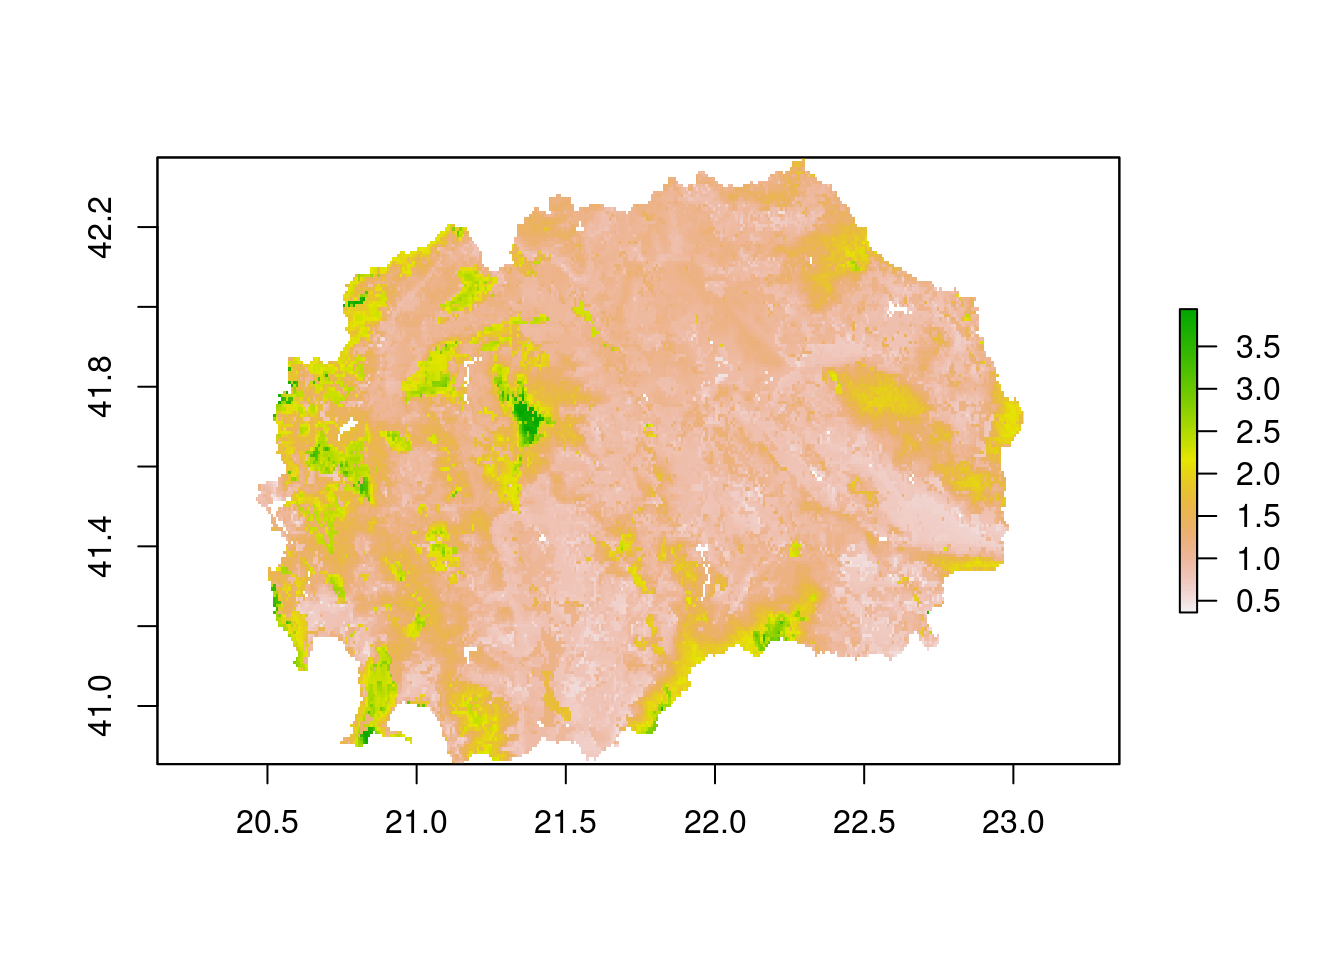
\includegraphics{SOCMapping_files/figure-latex/unnamed-chunk-80-1.pdf}
\caption{\label{fig:unnamed-chunk-80}Performance of the different svm models
in the parameter tuning procedure}
\end{figure}

\hypertarget{select-the-model-with-the-best-combination-of-epsilon-and-cost}{%
\subsubsection{Select the model with the best combination of epsilon and
cost}\label{select-the-model-with-the-best-combination-of-epsilon-and-cost}}

The best model is the one with the lowest mean squared error derived by
cross-validation. The parameters for the cross-validation can be defined
in the \texttt{tune.control()} function. By default, it uses
cross-validation using 10 folds.

\begin{Shaded}
\begin{Highlighting}[]
\CommentTok{# Choose the model with the best combination of epsilon and cost}
\NormalTok{tunedModel <-}\StringTok{ }\NormalTok{tuneResult}\OperatorTok{$}\NormalTok{best.model}

\KeywordTok{print}\NormalTok{(tunedModel)}
\end{Highlighting}
\end{Shaded}

\begin{verbatim}
## 
## Call:
## best.tune(method = svm, train.x = OCSKGM ~ ., data = dat@data[, 
##     c("OCSKGM", names(COV))], ranges = list(epsilon = seq(0.1, 
##     0.2, 0.02), cost = c(5, 7, 15, 20)))
## 
## 
## Parameters:
##    SVM-Type:  eps-regression 
##  SVM-Kernel:  radial 
##        cost:  5 
##       gamma:  0.03448276 
##     epsilon:  0.2 
## 
## 
## Number of Support Vectors:  2193
\end{verbatim}

\hypertarget{predict-the-ocs-using-the-model}{%
\subsubsection{Predict the OCS using the
model}\label{predict-the-ocs-using-the-model}}

\begin{Shaded}
\begin{Highlighting}[]
\CommentTok{# Use the model to predict the SOC in the covariates space}
\NormalTok{OCSsvm <-}\StringTok{ }\KeywordTok{predict}\NormalTok{(COV, tunedModel)}

\CommentTok{# Save the result}
\KeywordTok{writeRaster}\NormalTok{(OCSsvm, }\DataTypeTok{filename =} \StringTok{"results/MKD_OCSKGM_svm.tif"}\NormalTok{,}
            \DataTypeTok{overwrite=}\OtherTok{TRUE}\NormalTok{)}

\KeywordTok{plot}\NormalTok{(OCSsvm)}
\end{Highlighting}
\end{Shaded}

\begin{figure}
\centering
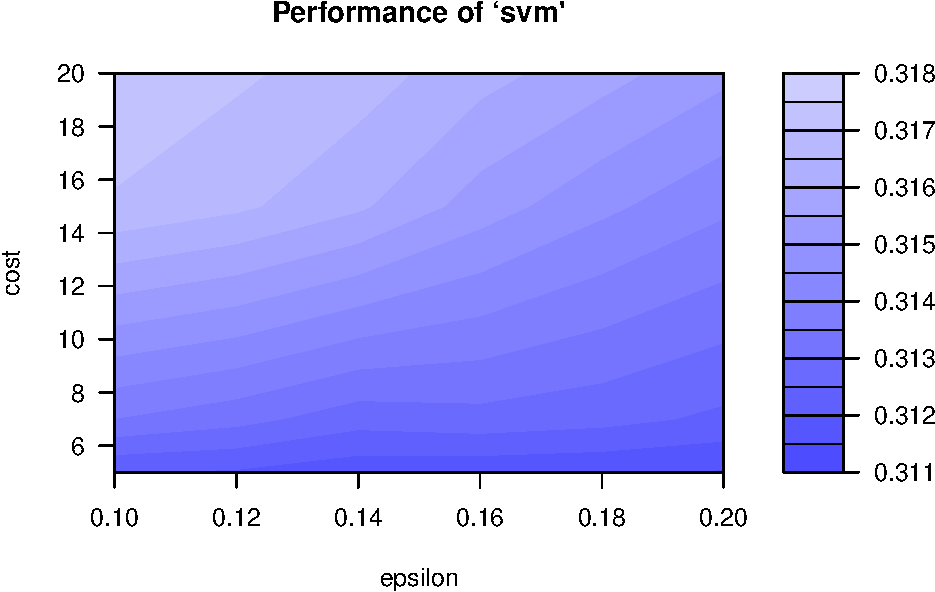
\includegraphics{SOCMapping_files/figure-latex/unnamed-chunk-82-1.pdf}
\caption{\label{fig:unnamed-chunk-82}SOC prediction using a support vector
machines model}
\end{figure}

Finally, we can evaluate the contribution of each covariate to the model
\citep{guyon2003introduction}:

\begin{Shaded}
\begin{Highlighting}[]
\CommentTok{# Variable importance in svm. Code by:}
\CommentTok{# stackoverflow.com/questions/34781495}

\NormalTok{w <-}\StringTok{ }\KeywordTok{t}\NormalTok{(tunedModel}\OperatorTok{$}\NormalTok{coefs) }\OperatorTok\StringTok{ }\NormalTok{tunedModel}\OperatorTok{$}\NormalTok{SV     }\CommentTok{# weight vectors}
\NormalTok{w <-}\StringTok{ }\KeywordTok{apply}\NormalTok{(w, }\DecValTok{2}\NormalTok{, }\ControlFlowTok{function}\NormalTok{(v)\{}\KeywordTok{sqrt}\NormalTok{(}\KeywordTok{sum}\NormalTok{(v}\OperatorTok{^}\DecValTok{2}\NormalTok{))\})  }\CommentTok{# weight}

\NormalTok{w <-}\StringTok{ }\KeywordTok{sort}\NormalTok{(w, }\DataTypeTok{decreasing =}\NormalTok{ T)}
\KeywordTok{print}\NormalTok{(w)}
\end{Highlighting}
\end{Shaded}

\begin{verbatim}
##      B04CHE3     soilmap6      TMDMOD3     soilmap7     soilmap1 
## 6.712914e+01 4.443748e+01 4.010740e+01 3.928593e+01 3.882377e+01 
##      DEMENV5      PRSCHE3      B07CHE3      LCEE103     soilmap2 
## 3.824383e+01 3.350877e+01 3.107515e+01 2.646657e+01 2.478332e+01 
##    soilmap19      LCEE104    soilmap16      LCEE101     soilmap5 
## 2.441025e+01 1.529174e+01 1.448675e+01 1.324205e+01 1.309922e+01 
##    soilmap15      LCEE102     soilmap4    soilmap20     soilmap9 
## 1.295171e+01 1.175225e+01 8.849019e+00 8.166970e+00 6.701250e+00 
##    soilmap10     soilmap3    soilmap17    soilmap12     soilmap8 
## 6.046196e+00 5.059617e+00 4.705567e+00 3.552720e+00 2.691221e+00 
##    soilmap18    soilmap14    soilmap11    soilmap13 
## 5.275093e-01 1.498048e-01 7.365523e-02 1.110223e-15
\end{verbatim}

svm is a powerful technique which represent another welcome possibility
to generate reliable and interpretable SOC predictions across different
scales of data availability, including country-specific SOC maps.

\hypertarget{chvalidation}{%
\chapter{Validation}\label{chvalidation}}

\emph{B Kempen, DJ Brus \& GBM Heuvelink}

\hypertarget{what-is-validation}{%
\section{What is Validation?}\label{what-is-validation}}

No map is perfect. All maps, including soil maps, are representations of
reality that are often based on an underlying model. This means that
there will always be a deviation between the phenomenon depicted on the
map and the phenomenon observed in the real world, i.e.~each map will
contain errors. The magnitude of the errors determines the quality of
the map. If a map matches reality well (the error is small), the quality
or accuracy of the map is high. On the other hand, if a map does not
match reality well, map accuracy is low.

Soil maps are used for many purposes. For example to report on (changes
in) soil organic carbon stocks, as input in agro-environmental models,
to determine land use suitability or for decision- and policy-making. It
is therefore, important that the quality of a map is determined and
quantified. This is achieved through (statistical) validation.

Validation is defined here as an activity in which the soil map
predictions are compared with observed values. From this comparison, the
map quality can be quantified and summarized using map quality measures.
These measures indicate how accurate the map is on average for the
mapping area, i.e.~what is the expected error at a randomly selected
location in the mapping area. This means that map quality measures
obtained through validation are global measures: each quality measure
gives one value for the entire map. Note that this is different from
results obtained through uncertainty assessment. Such assessment
provides local, location-specific (i.e.~for each individual grid cell)
estimates of map quality as we saw in the previous sections. Another
important difference between validation and uncertainty assessment is
that validation can be done using a model-free approach. Uncertainty
assessment takes a model-based approach by defining a geostatistical
model of the soil property of interest and deriving an interpolated map
and the associated uncertainty from that, or by constructing a
geostatistical model of the error in an existing map. The approach
yields a complete probabilistic characterization of the map uncertainty,
but such characterization is only valid under the assumptions made; for
instance, the stationarity assumptions required for kriging. Validation,
when done properly as explained hereafter, does not assume a
geostatistical model of the error, and hence is model- or
assumption-free. This is an important property of validation since we do
not want to question the objectivity and validity of the validation
results.

We distinguish internal and external map accuracy. Statistical methods
typically produce direct estimates of map quality, for instance, the
kriging variance or the coefficient of determination (\({R^2}\)) of a
linear regression model. These we refer to as internal accuracy measures
since these rely on model assumptions and are computed from data that
are used for model calibration. Preferably, validation is done with an
independent dataset not used in map making. Using such dataset gives the
external map accuracy. One will often see that the external accuracy is
poorer than the internal accuracy.

In section 8.3.2 we will present the most common accuracy measures used
to quantify map quality of quantitative (continuous) soil maps and
qualitative (categorical) soil maps. In section 8.3.3 we will introduce
three commonly used validation methods and show how to estimate the map
quality measures from a sample. This chapter is largely based on
\citet{brus2011sampling}. For details, please refer to this paper.

\hypertarget{map-quality-measures}{%
\section{Map Quality Measures}\label{map-quality-measures}}

\hypertarget{quality-measures-for-quantitative-soil-maps}{%
\subsection{Quality Measures for Quantitative Soil
Maps}\label{quality-measures-for-quantitative-soil-maps}}

All map quality measures considered here are computed from the
prediction error. For quantitative soil maps of continuous soil
properties (e.g.~organic carbon content, pH, clay content) the
prediction error is defined as the difference between the predicted
value at a location and the true value at that location (which is the
value that would be observed or measured by a preferably errorless
measurement instrument) \citep{brus2011sampling}:

\begin{equation}
e(s) = \hat{Z}(s) - Z(s)
\end{equation}

where \({\hat{Z}(s)}\) is the predicted soil property at validation
location s, and \({Z(s)}\) is the true value of the soil property at
that location. We consider six map quality measures that are computed
from the prediction error here: the mean error, the mean absolute error,
the mean squared error and root mean squared error, the model
efficiency, and the mean squared deviation ratio.

Before we introduce the map quality measures and show how to estimate
these, it is important to understand the difference between the
population and a sample taken from the population. The population is the
set of all locations in a mapping area. For digital soil maps, this is
the set of all pixels or grid cells of a map. A sample is a subset of
locations, selected in some way from the set of all locations in the
mapping area. With validation we want to assess the map accuracy for the
entire population, i.e.~for the map as a whole; we are not interested in
the accuracy at the sample of locations only. For instance, we would
like to know the prediction error averaged over all locations of a map
and not merely the average prediction error at a sample of locations.
Map quality measures are, therefore, defined as population means.
Because we cannot afford to determine the prediction error at each
location (grid cell) of the mapping area to calculate the population
means, we have to take a sample of a limited number of locations in the
mapping area. This sample is then used to estimate the population means.
It is important to realize that we are uncertain about the population
means because we estimate it from a sample. Ideally, this uncertainty is
quantified and reported together with the estimated map quality
measures.

In this section, we will introduce the definitions of the map quality
measures. In the next section, we show how we can estimate these
measures from a sample.

\textbf{Mean error}

The mean error (\({ME}\)) measures bias in the predictions. The \({ME}\)
is defined as the population mean (spatial mean) of the prediction
errors:

\begin{equation}
M E = e = \frac{1}{N} \sum_{i=1}^{N} e (s_i)
\end{equation}

where \(i\) indicates the location, \({i = 1, 2,\dots N}\), and \(N\) is
the total number of locations or grid cells/pixels in the mapping area.
The mean error should be (close to) zero, which means that predictions
are unbiased meaning that there is no systematic over- or
under-prediction of the soil property of interest.

\textbf{Mean absolute error and (root) mean squared error}

The mean absolute error (\({MAE}\)) and mean squared error (\({MSE}\))
are measures of map accuracy and indicate the magnitude of error we make
on average. The \({MAE}\) is defined by the population mean of the
absolute errors:

\begin{equation}
M A E = |\underline{e}| = \frac{1}{N} \sum_{i=1}^{N} \underline{e} (s_i)
\end{equation}

and the \({MSE}\) by the population mean of the squared errors:

\begin{equation}
M S E = \underline{e}^2 = \frac{1}{N} \sum_{i=1}^{N} \underline{e}^2 (s_i)
\end{equation}

Many authors report the root mean squared error (\({RMSE}\)) instead of
the \({MSE}\), which is computed by taking the square root of the
\({MSE}\). The \({RMSE}\) can be a more appealing quality measure since
it has the same unit of measurement as the mapped property and can,
therefore, more easily be compared to it. If the squared error
distribution is strongly skewed, for instance when several very large
errors are present, then this can severely inflate the (R)MSE. In such
case, the (root) median squared error is a more robust statistic for the
`average' error \citep{kempen2012efficiency}.

\citet{brus2011sampling} argue that instead of using a single summary
statistic (the mean) to quantify map quality measures, one should
preferably express quality measures for quantitative soil maps through
cumulative distribution functions (CDFs). Such functions provide a full
description of the quality measures from which various parameters can be
reported, such as the mean, median or percentiles. Furthermore, they
argue that it can be of interest to define CDFs or its parameters for
sub-areas, for instance, geomorphic units, soil or land cover classes.
\citet{brus2011sampling} give examples of estimating CDFs for validation
of digital soil maps.

\textbf{Amount of variance explained}

The model efficiency, or Amount of Variance Explained (\({AVE}\))
\citep[\citet{samuel2015more}]{angelini2016mapping}, quantifies the
fraction of the variation in the data that is explained by the
prediction model. It measures the improvement of the model prediction
over using the mean of the data set as predictor and is defined as
follows \citep{krause2005comparison}:

\begin{equation}
A V E = 1 -  \frac{\sum_{i=1}^{N} (\hat{Z}(s_i) - Z(s_i))^2}{\sum_{i=1}^{N}  (Z(s_i) - \underline{Z})^2}
\end{equation}

where \({\underline{Z}}\) is the population mean of soil property \(Z\).
The quantity in the numerator is the sum of the squared prediction
errors (for each location the prediction error is computed and squared;
the squared prediction errors are summed over all locations in the
area). In linear regression, this quantity is known as the residual sum
of squares (\({RSS}\)). The quantity in the denominator is also a sum of
squared prediction errors, but here the mean of the area is used as a
predictor. In linear regression, this quantity is known as the total sum
of squares (\({TSS}\)). Note that if we would divide the quantity in the
denominator by the number of locations in the mapping area \(N\) we
would obtain the population variance (spatial variance) of the soil
property \(Z\).

If the numerator and denominator are equal, meaning the \({AVE}\) is
zero, then the model predictions are no improvement over using the mean
of the data set as a predictor for any location in the mapping area. An
\({AVE}\) value larger than zero (\({RSS}\) smaller than \({TSS}\))
means that the model predictions are an improvement over using the mean
as a predictor (this is what we hope for). In case the \({AVE}\) is
negative, then the mean of the data set is a better predictor than the
prediction model.

\textbf{Mean squared deviation ratio}

Finally, we introduce the mean squared deviation ratio (\({MSDR}\)) as a
map quality measure \citep[\citet{lark2000comparison},
\citet{voltz1990comparison},
\citet{webster_2007}]{kempen2010pedometric}. Contrary to the quality
measures discussed so far, the \({MSDR}\) assesses how well the
prediction model estimates the prediction uncertainty (expressed as the
prediction error variance). The \({MSDR}\) is defined as:

\begin{equation}
M S D R = \frac{1}{N} \sum_{i=1}^{N} \frac{(\hat{Z}(s_i) - Z(s_i))^2}{\sigma^2(s_i)}
\end{equation}

where \({\sigma^2(s_i)}\) is the prediction error variance at location
\({s_i, i = 1, 2, \dots N}\). The numerator is the squared error at
location \({s_i}\). The fraction represents the squared \({Z_{score}}\).
In case of kriging, the prediction error variance is the kriging
variance. In case of linear regression, the prediction error variance is
the prediction variance of the linear regression predictions that can be
obtained by the statistical software R by running the predict function
with argument \({se.fit = TRUE}\). This function returns for each
prediction location the standard error of the predicted value as well as
the residual standard deviation (the residual.scale value). By squaring
both values and then summing these, the prediction error variance is
obtained. If the prediction model estimates the error variance well,
then the \({MSDR}\) should be close to one. A value smaller than one
suggests that the prediction error variance overestimates the variance;
a value larger than one suggests that the prediction error variance
underestimates the variance.

\citet{lark2000comparison} notes that outliers in the prediction data
will influence the squared \({Z_{score}}\) and suggests to use the
median squared \({Z_{score}}\) instead of the mean since it is a more
robust estimator. A median squared \({Z_{score}}\) equal to 0.455
suggests that the prediction model estimates the prediction uncertainty
well.

\hypertarget{quality-measures-for-qualitative-soil-maps}{%
\subsection{Quality Measures for Qualitative Soil
Maps}\label{quality-measures-for-qualitative-soil-maps}}

Like the quality measures for quantitative soil maps, the quality
measures for qualitative or categorical soil maps (e.g.~soil classes)
are defined for the population, i.e.~all locations in the mapping area.
The basis for map quality assessment of qualitative maps is the error
matrix \citep[\citet{lark1995components}]{brus2011sampling}. This matrix
is constructed by tabulating the observed and predicted class for all
locations in the mapping area in a two-way contingency table. The
population error matrix is a square matrix of order \(U\), with \(U\)
being the number of soil classes observed and mapped. The columns of the
matrix correspond to observed soil classes and the rows of predicted
soil classes (the map units).\(N\) is the total number of locations of
the mapping area. Elements \(N_{ij}\) are the number of locations mapped
as class \(i\) with observed class \(j\). The row margins \(N_{i+}\) are
the locations mapped as class \(i\), and column margins \(N_{+j}\) the
locations for which the observed soil class is \(j\). Note that the
elements of the population error matrix can also be interpreted as
surface areas. In that case element \(N_{ij}\) is the surface area
mapped as class \(i\) with observed class \(j\).

From the population error matrix, several quality measures can be
summarized, though it is strongly recommended that the error matrix is
included in a validation assessment. \citet{brus2011sampling} follow the
suggestion by \citet{stehman1997selecting} that quality measures for
categorical maps should be directly interpretable in terms of the
probability of a misclassification and therefore recommend the use of
three map quality measures: the overall purity, the map unit purity, and
class representation. We follow this recommendation here. Note that the
map unit purity often is referred to as user's accuracy, and class
representation as producer's accuracy
\citep[\citet{adhikari2014constructing}]{stehman1997selecting}.
\citet{lark1995components} however, questions the appropriateness of
these terms since both quality measures can be important for users as
well as producers. He proposes to use map unit purity and class
representation instead, which is adopted by \citet{brus2011sampling} and
followed here.

A fourth frequently used group of quality measures are Kappa indices,
which adjust the overall purity measure for hypothetical chance
agreement \citep{stehman1997selecting}. How this chance agreement is
defined differs between the various indices. Some authors, however,
conclude that Kappa indices are difficult to interpret, not informative,
misleading and/or flawed and suggest to abandon their use
\citep{pontius2011death}. These authors argue that Kappa indices attempt
to compare accuracy to a baseline of randomness, but randomness is not a
reasonable alternative for map construction. We, therefore, do not
consider kappa here.

The overall purity is the fraction of locations for which the mapped
soil class equals the observed soil class and is defined as
\citep{brus2011sampling}:

\begin{equation}
\rho = \sum_{i=1}^{U} N_{uu} / N
\end{equation}

which is the sum of the principal diagonal of the error matrix divided
by the total number of locations in the mapping area. The overall purity
can be interpreted as the areal proportion of the mapping area that is
correctly classified.

Alternatively, an indicator approach can be used to compute the overall
purity. A validation site gets a `1' if the observed soil class is
correctly predicted and a `0' otherwise. The overall purity is then
computed by taking the average of the indicators.

\textbf{Map unit purity}

The map unit purity is calculated from the row marginals of the error
matrix. It is the fraction of validation locations with mapped class
\(u\) for which the observed class is also \(u\). The map unit purity
for class \(u\) is defined as \citep{brus2011sampling}:

\begin{equation}
\rho_u = \frac{ N_{uu}}{N_{u+}}
\end{equation}

The map unit purity can be interpreted as the proportion of the area of
the map unit that is correctly classified. The complement of \(\rho_u\),
\(1 - \rho_u\), is referred to as the error of commission for mapped
class \(u\).

\textbf{Class representation}

The class representation is calculated from the column marginals of the
error matrix. It is the fraction of validation locations with observed
class \(u\) for which the mapped class is \(u\). The class
representation for class \(u\) is defined as \citep{brus2011sampling}:

\begin{equation}
r_u = \frac{ N_{uu}}{N_{+u}}
\end{equation}

The class representation can be interpreted as the proportion of the
area where in reality class \(u\) occurs that is also mapped as class
\(u\). The complement of \(r_u\), \(1 - r_u\), is referred to as the
error of omission for mapped class \(u\).

\hypertarget{estimating-the-map-quality-measures-and-associated-uncertainty}{%
\subsection{Estimating the Map Quality Measures and Associated
Uncertainty}\label{estimating-the-map-quality-measures-and-associated-uncertainty}}

In validation, we estimate the population means of the map quality
measures from a sample taken from a limited number of locations in the
mapping area. After all, we cannot afford to sample all locations,
i.e.~each grid cell of our soil map. Because the map quality measures
are estimates, we are uncertain about these: we infer the quality
measures from only a limited number of observations taken from the
population. We do not know the true population means. The estimation
uncertainty can be quantified with the sampling variance. From the
variance, the lower and upper boundary of a confidence interval,
typically the \(95\%\), can be computed using basic statistical theory:

\begin{equation}
CI = (\underline{\hat{x}} - 1.96x \frac{\sigma}{\sqrt{n} } ; \underline{\hat{x}} + 1.96x \frac{\sigma}{\sqrt{n} })
\end{equation}

where \(x\) is the estimated map quality measure, for instance, the
\(ME\), \(MSE\) or overall purity, \(\sigma\) is the estimated standard
deviation of the map quality measure and \(n\) is the validation sample
size.

Quantified information about the uncertainty associated to map quality
measures is useful and required for statistical testing. For instance,
if one wants to test if one mapping method performs better than the
other method one needs quantified information about uncertainty. Because
we are uncertain about the estimated quality measures, an observed
difference in map quality between two methods does not necessarily mean
that one method is better than the others, even when there is a
substantial difference. The difference might be attributed to chance
because we infer the quality measures from a limited sample from the
population. With statistical hypothesis testing, we can calculate how
large the probability is that observed difference is caused by chance.
Based on the outcome we can accept or reject the hypothesis that there
is no difference between the performance of two mapping methods (this
would be the null hypothesis for statistical testing) for a given
significance level, usually 0.05.

\hypertarget{graphical-map-quality-measures}{%
\section{Graphical Map Quality
Measures}\label{graphical-map-quality-measures}}

In addition to quantifying map accuracy statistically, one can also
present validation results obtained from a sample graphically. This can
be done by creating scatter plots of predicted against observed values
and spatial bubble plots of validation errors. Figure
\ref{fig:rwandaval} shows an example of a scatterplot and bubble plot.
Both plots can be easily made with R \citep{rcore}. Use the function
plot(x,y)to generate a scatter plot. The 1:1 line (black line in Figure
\ref{fig:rwandaval}) can be added to the plot with the command
\texttt{abline(0,1)}. The spatial bubble plot can be generated with the
bubble function of the sp package \citep{pebesma2005classes}.

\begin{figure}
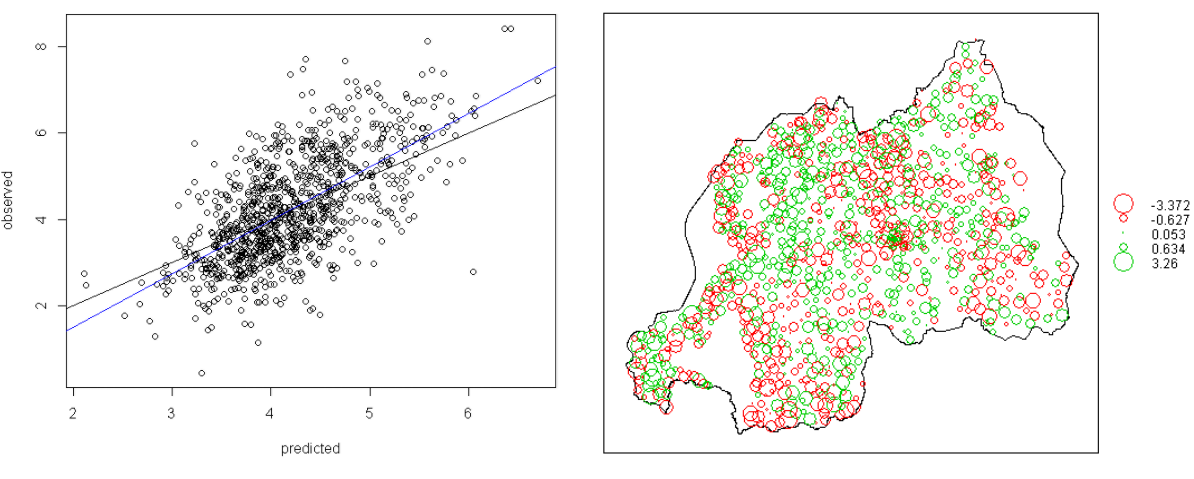
\includegraphics[width=0.8\linewidth]{images/Validation_Rwanda} \caption{Scatterplot of predicted versus observed soil organic matter content for Rwanda (left) and spatial bubble plot of cross-validation error for soil organic matter (right) (Kempen et al., 2015). The black line in the scatter plot represents the 1:1 line of prediction versus observed, the blue line represents the regression between observed and predicted values}\label{fig:rwandaval}
\end{figure}

\hypertarget{validation-methods-and-statistical-inference}{%
\section{Validation Methods and Statistical
Inference}\label{validation-methods-and-statistical-inference}}

Following \citet{brus2011sampling}, we introduce and discuss three
common validation methods: additional probability sampling,
data-splitting and cross-validation, and show how to estimate the map
quality measures introduced in the previous section from a sample.

With additional probability sampling, an independent dataset is
collected from the sampling population (all grid cells of a digital soil
map) for the purpose of validation. This dataset is used in addition to
a dataset that is used to calibrate a prediction model. Such dataset is
often a legacy dataset collected with a purposive sampling design.

Data-splitting and cross-validation are applied in situations where one
has only one data set available for prediction model calibration and
validation. This can be a dataset collected with probability sampling,
but in practice this typically is a legacy dataset collected with some
purposive sampling design.

We warn here that if one uses data-splitting or cross-validation with a
dataset collected with purposive sampling, then this has severe
implications on the validity and interpretation of the estimated map
quality measures as we will explain below

\hypertarget{additional-probability-sampling}{%
\subsection{Additional Probability
Sampling}\label{additional-probability-sampling}}

The most appropriate approach for validation is by additional
probability sampling. This means that an independent validation dataset
is collected in the field on basis of a probability sampling design.
Validation based on probability sampling ensures one obtains unbiased
and valid estimates of the map quality measures
\citep[\citet{stehman1999basic}]{brus2011sampling}. Additional
probability sampling has several advantages compared to data-splitting
and cross-validation using non-probability sample data. These are:

\begin{itemize}
\item
  no model is needed for estimating map quality estimates. We can apply
  design-based estimation, meaning that model-free unbiased and valid
  estimates of the map quality measures can be obtained;
\item
  discussions on the validity of the estimated map quality are avoided;
\item
  model-free, valid estimates of the variance of the map quality
  measures can be obtained that allows for hypothesis testing, e.g.~for
  comparison of model performance.
\end{itemize}

Disadvantages can be extra costs involved in collecting an additional
sample or terrain conditions that make it difficult to access all
locations in the mapping area. Probability sampling is random sampling
such that:

\begin{itemize}
\item
  all locations in the mapping area have a probability larger than 0 of
  being selected
\item
  the inclusion probabilities are known but need not be equal.
\end{itemize}

It should be noted that random sampling is often used for arbitrary or
haphazard sampling. Such sampling is not probability sampling because
the inclusion probabilities are not known. Design-based, model-free
estimation of map quality measures is not possible in this case. All
probability samples are random samples but not all random samples are
probability samples. The term probability sampling should therefore only
be used for random sampling with known inclusion probabilities.

There are many different probability sampling designs: simple,
stratified, systematic, two-stage, clustered random sampling. We will
not give an exhaustive overview here of all these designs. A good
resource is \cite{de2006sampling}. For reasons of simplicity, we focus
here on simple random sampling.

In simple random sampling, no restrictions are imposed on the random
selection of sampling sites except that the sample size is fixed and
chosen prior to sampling \citep{de2006sampling}. All sampling locations
are selected with equal probability and independently from each other.
This can, for instance, be done as follows \citep{de2006sampling}:

\begin{enumerate}
\def\labelenumi{\arabic{enumi}.}
\item
  Determine the minimum and maximum \(X\) and \(Y\) coordinates of the
  mapping area (the bounding box).
\item
  Generate two independent random coordinates \(X\) and \(Y\) from a
  uniform probability distribution on the interval (\(x_{min}\),
  \(x_{max}\)) and (\(y_{min}\), \(y_{max}\))
\item
  Check if the selected sampling site falls within the mapping area.
  Accept the sampling site if it does; discard the sampling site if it
  does not.
\item
  Repeat steps 2 and 3 until the \(n\) locations have been selected.
\end{enumerate}

If a sampling location cannot be visited because of inaccessibility for
instance, then this location should be discarded and be replaced by a
location chosen from a reserve list. Always the location at the top of
the list should be selected for this purpose; not an arbitrarily chosen
location from the list such as the closest one. It is not allowed to
shift an inaccessible sampling location to a location nearby that can be
accessed. Irregularity, clustering and open spaces characterize the
simple random sampling design \citep{de2006sampling}.

\textbf{Estimation of quantitative map quality measures:} For each
validation location we compute the error, \(e(s_i)\), the absolute
error, \(|e|(s_i)\), or squared error, \(e^2(s_i)\). The spatial mean of
the mapping area for map quality measure \(x\) is then estimated by:

\begin{equation}
e(s_i) = \hat{Z}(s_i) - Z(s_i)
\end{equation}

\begin{equation}
|e|(s_i) = |\hat{Z}(s_i) - Z(s_i)|
\end{equation}

\begin{equation}
e^2(s_i) =( \hat{Z}(s_i) - Z(s_i))^2
\end{equation}

\begin{equation}
\underline{\hat{x}} = \frac{1}{N} \sum_{i=1}^{N} x(s_i)
\end{equation}

where \(i\) indicates the validation location, \(i = 1, 2, \dots, n\),
\(n\) the validation sample size, and \(x_{si}\) the estimated
population mean of map quality measure \(x\) at location \(s_i\). \(x\)
is the prediction error in case of the \(ME\), absolute error in case of
the \(MAE\), squared prediction error in case of the \(MSE\). Note that
the estimator is the unweighted sample mean. This unweighted mean is an
unbiased estimator because all sampling locations were selected with
equal probability.

The \(MSDR\) is estimated by:

\begin{equation}
\widehat{M S D R} = \frac{1}{N} \sum_{i=1}^{n} \frac{(\hat{Z}(s_i) - Z(s_i))^2}{\sigma^2(s_i)}
\end{equation}

and the \(AVE\) by:

\begin{equation}
\widehat{A V E} = 1 - \frac{\sum_{i=1}^{n} (\hat{Z}(s_i) - Z(s_i))^2}{ \sum_{i=1}^{n} (Z(s_i) -  \underline{\hat{Z}})^2}
\end{equation}

where \(\underline{\hat{Z}}\) is the mean of the target soil property
estimated from the validation sample.

One should be careful when assessing the proportion of variance
explained by computing the \(R^2\) from a linear regression of the
predicted value on the observed value \citep{krause2005comparison}, as
is often done in practice. The \(R^2\) quantifies the dispersion around
the regression line; not around the 1:1 line in which we are interested
in validation. So it does not directly compare the predicted with
observed value as does the \(AVE\); i.e.~it is not based on the
prediction error. A high \(R^2\)-value, therefore, does not
automatically mean a high \(AVE\). For instance, in case of strongly
biased predictions the \(R^2\) can be high but the \(AVE\) will be low.
The blue line in Figure \ref{fig:rwandaval} is the regression line that
one obtains when regression the observed value of the predicted value.
This line slightly differs from the 1:1 line. In this example, the
\(R^2\) of the regression is 0.42 while the \(AVE\) is 0.40. The
uncertainty associated to the estimated map quality measures is
quantified with the sampling variance, which for the \(ME\), \(MAE\) and
\(MSE\) is estimated by:

\begin{equation}
Var(\underline{\hat{x}}) = \frac{1}{n(n-1)} \sum_{i=1}^{n} (x(s_i) -  \underline{\hat{x}})
\end{equation}

and the \(95\%\) confidence interval (\(CI\)) of \(x\) is given by:

\begin{equation}
CI_{95} = \underline{\hat{x}} \pm 1.96x\sqrt{Var(\underline{\hat{x}})}
\end{equation}

We should warn here that the calculation of the \(CI\) is based on the
assumption that the estimated map quality measure means have a normal
distribution (the central limit theorem). For the squared errors this
assumption can be unrealistic, especially for small sample sizes.

\textbf{Estimation of qualitative map quality measures:} For validation
of qualitative soil maps, a sample error matrix is constructed from the
validation data (Figure \ref{fig:errormatrix}). \(n\) is the total
number of validation locations in the sample. Element \(n_{ij}\) of the
matrix corresponds to the number of validation locations that have been
predicted as class \(i\), \(i = 1, 2, \dots U\) and belong to class
\(j\), \(j = 1, 2, \dots U\) \citep{lark1995components}. The matrix
summarizes correct predictions and incorrect predictions within the
validation data.

\begin{figure}

{\centering 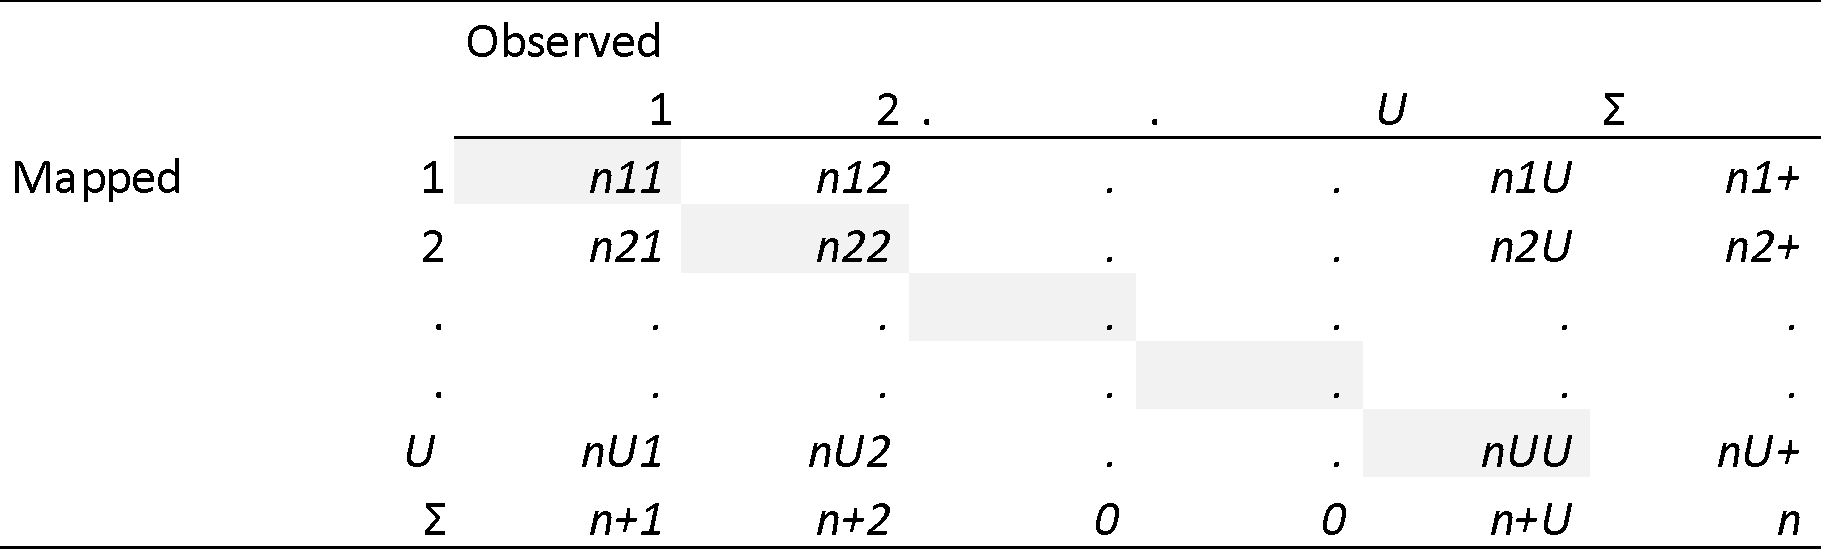
\includegraphics[width=0.8\linewidth]{images/Validation_error_matrix} 

}

\caption{Sample error matrix}\label{fig:errormatrix}
\end{figure}

From the sample error matrix the overall purity, map unit purity and
class representation are estimated by:

\begin{equation}
\hat{\rho} = \sum_{i=1}^{U} n_{uu} / n
\end{equation}

\begin{equation}
\hat{\rho}_u = \frac{ n_{uu}}{n_{u+}}
\end{equation}

\begin{equation}
\hat{r_u} = \frac{ n_{uu}}{n_{+u}}
\end{equation}

Alternatively, the overall purity can be estimated by defining a purity
indicator variable for each validation location that takes value 1 if
the mapped soil class equals the observed soil class at that location,
and 0 else. The overall purity is then estimated by:

\begin{equation}
\hat{\rho} = \frac{1}{n} \sum_{i=1}^{n} \partial(s_i)
\end{equation}

where \({\delta(s_i)}\) is the indicator variable at validation location
\(s_i\). The variance of the estimated overall purity is estimated by:

\begin{equation}
Var(\hat{\rho}) = \frac{1}{n(n-1)} \sum_{i=1}^{n} (\partial(s_i) - \hat{\rho})^2
\end{equation}

Alternatively, the variance is estimated by:

\begin{equation}
Var(\hat{\rho}) = \frac{\hat{\rho}(1 - \hat{\rho})}{n - 1)}
\end{equation}

which is the variance of a binomial probability distribution. The
\(95\%\) confidence interval of \(\hat{\rho}\) is given by:

\begin{equation}
CI_{95} = \hat{\rho} \pm 1.96x \sqrt{Var(\hat{\rho})}
\end{equation}

We warn that the \(CI\) as calculated here is a rough approximation
which only holds when \(n \times \hat{\rho}\) and
\(n \times (1 - \hat{\rho})\) are large (5 as a rule of thumb).
Otherwise, the binomial distribution should be used to compute the
\(CI\). Figure \ref{fig:errormatrix2} shows a hypothetical example of a
sample error matrix for soil class map. For this example, the overall
purity is estimated by:

\begin{equation}
\hat{\rho} = \frac{(19 + 33 + 25 + 42 + 19)}{240} = 0.575
\end{equation}

meaning that for an estimated \(57.5\%\) of the mapping area the mapped
soil class is equal to the true soil class.

\begin{figure}

{\centering 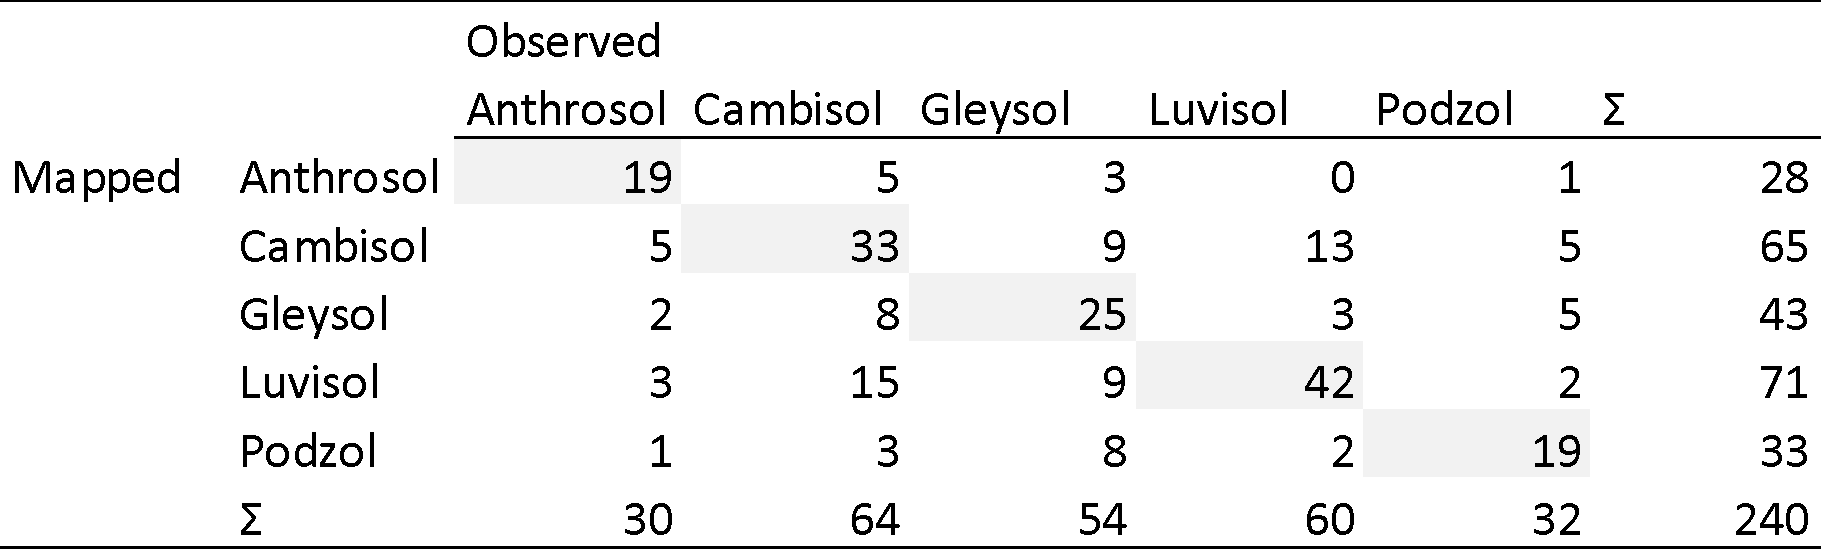
\includegraphics[width=0.8\linewidth]{images/Validation_error_matrix2} 

}

\caption{Sample error matrix for a hypothetical soil class map}\label{fig:errormatrix2}
\end{figure}

Table \ref{tab:purity} gives the map unit purities and class
representations for this example. The map unit purity of the Gleysol is
0.581, meaning that at \(58.1\%\) of the validation locations for which
a Gleysol is predicted, a Gleysol is observed. Assuming the validation
data were collected by simple random sampling, we could conclude that
for \(58.1\%\) of the area mapped as Gleysol we would find a Gleysol in
the field. The class representation of the Gleysol is 0.463, meaning
that for \(46.3\%\) of the validation locations classified as Gleysol,
we map a Gleysol. The majority of the Gleysol locations is thus mapped
as a different soil class. Again, assuming the validation data were
collected by probability sampling, we would estimate that \(22.5\%\)
(\(\frac{54}{240}\) \(\times\) \(100\%\)) of our mapping area is covered
by Gleysols. We map Gleysols for \(17.9\%\) of the area
(\(\frac{43}{240}\) \(\times\) \(100\%\)). It can happen that a soil
class has a high map unit purity and a low-class representation. This
means that if we map a Gleysol we will likely find a Gleysol there, but
that a large extent of the true Gleysol area is not mapped as such.

\begin{table}

\caption{\label{tab:purity}Map unit purity and class representation statistics for an hypothetical example.}
\centering
\begin{tabular}[t]{lrr}
\toprule
unit & map.unit.purity & class.representation\\
\midrule
Anthrosol & 0.679 & 0.633\\
Cambisol & 0.508 & 0.516\\
Gleysol & 0.508 & 0.463\\
Luvisol & 0.592 & 0.700\\
Podzol & 0.576 & 0.594\\
\bottomrule
\end{tabular}
\end{table}

\hypertarget{data-splitting}{%
\subsection{Data-Splitting}\label{data-splitting}}

In data-splitting, the sample data set is split into two subsets. One
subset is used to calibrate the prediction model. The other subset is
used for validation. A frequently used splitting criterion is 70-30,
where \(70\%\) of the sample data are used for calibration and \(30\%\)
for validation. The choice of a splitting criterion, however, is
arbitrary and it is not evident how to split a data set in such a way
that unbiased and valid estimates of the map accuracy can be obtained.
For sparse data sets, data-splitting can be inefficient since the
information in the data set is not fully exploited for both calibration
and validation.

It is important to note here that a random subsample of (legacy) data
that are collected with a purposive (non-probability) design, is not a
probability sample of the study area. This means that design-based
estimation of map quality measures is not possible.

Thus, we will not obtain model-free, unbiased and valid estimates of the
quality measures from non-probability sample validation data. In a case
study, \citet{knotters2013purposive} showed that model-based predictions
of producer's accuracies from two models differed strongly, indicating
that with the model-based approach the validation results strongly
depend on model assumptions.

In most studies, however, spatial correlation is not accounted for when
estimating map quality measures using the estimators presented above
under `Simple random sampling' from non-probability sample data. In such
case, the quality measures cannot be considered unbiased and valid
estimates of the population means of the map quality measures. In
addition, the estimated variance of the map quality measures is not
valid and statistical testing of mapping methods to assess which method
gives the most accurate predictions cannot be done.

In other words, if the simple random sampling estimators are used to
estimate map quality measures then these are only valid for the
validation data points. The map quality measures do not give a valid
estimate of the quality of the map as a whole (the population). For
instance, the overall purity cannot be interpreted as an areal
proportion of correctly mapped soil classes, only as the proportion of
the validation data points for which the soil class is correctly
predicted. 70-30, where \(70\%\) of the sample data are used for
calibration and \(30\%\) for validation. The choice of a splitting
criterion, however, is arbitrary and it is not evident how to split a
data set in such a way that unbiased and valid estimates of the map
accuracy can be obtained. For sparse data sets, data-splitting can be
inefficient since the information in the data set is not fully exploited
for both calibration and validation.

It is important to note here that a random subsample of (legacy) data
that are collected with a purposive (non-probability) design, is not a
probability sample of the study area. This means that design-based
estimation of map quality measures is not possible.

If a validation (sub)sample is a non-probability sample of the mapping
area, then we must account for possible spatial autocorrelation of the
prediction errors when estimating the map quality measures. One can
imagine that when two validation locations are close together and the
prediction errors are correlated that there is less information in these
two locations (there is information redundancy because of
autocorrelation) than in two isolated locations. This information
redundancy has to be accounted for when estimating map quality measures
and implies that we have to rely on model-based estimation: a model for
the spatially autocorrelated prediction error has to be assumed. Thus,
we will not obtain model-free, unbiased and valid estimates of the
quality measures from non-probability sample validation data. In a case
study, Knotters and Brus (2013) showed that model-based predictions of
producer's accuracies from two models differed strongly, indicating that
with the model-based approach the validation results strongly depend on
model assumptions.

In most studies, however, spatial correlation is not accounted for when
estimating map quality measures using the estimators presented above
under `Simple random sampling' from non-probability sample data. In such
case, the quality measures cannot be considered unbiased and valid
estimates of the population means of the map quality measures. In
addition, the estimated variance of the map quality measures is not
valid and statistical testing of mapping methods to assess which method
gives the most accurate predictions cannot be done.

In other words, if the simple random sampling estimators are used to
estimate map quality measures then these are only valid for the
validation data points. The map quality measures do not give a valid
estimate of the quality of the map as a whole (the population). For
instance, the overall purity cannot be interpreted as an areal
proportion of correctly mapped soil classes, only as the proportion of
the validation data points for which the soil class is correctly
predicted.

\hypertarget{xval}{%
\subsection{Cross-Validation}\label{xval}}

In \(K\)-fold cross-validation (CV), the dataset is split into \(K\)
roughly equal sets. One of these sets is set aside for validation. The
model is then calibrated using the data from the \(K\)-1 sets and used
to predict the target variable for the data points set aside. From this
prediction, the prediction error is calculated. This procedure is
repeated \(K\) times, each time setting a different set aside for
validation. In this way, we obtain \(K\) estimates of the prediction
error: one for each validation sample site. In this way, all data are
used for validation and model calibration. It is thus much more
efficient than data-splitting.

\(K\) is typically chosen as 5 or 10 or as \(N\) the number of data
points. The latter is referred to as leave-one-out cross-validation
(LOOCV) in which only one validation site is set aside in each
iteration. The model is then calibrated with \(N\)-1 observations. Some
repeat \(K\)-fold cross-validation a number of times and average the
results to obtain a more robust estimate of the map quality measures.

Note that the problem of spatially correlated errors remains when data
are non-probability sample data. Cross-validation using a
non-probability sampling dataset suffers from the same drawbacks with
respect to unbiasedness and validity of the estimates of the map quality
measures as data-splitting. The estimates cannot be interpreted as being
valid for the mapping area, but only for the validation locations.

In R, the caret package \citep{kuhn2016short} offers functionality for
data-splitting and cross-validation.

\hypertarget{TS:validation}{%
\section{Technical steps - Validation}\label{TS:validation}}

\emph{GF Olmedo}

\hypertarget{prediction-error}{%
\subsection{Prediction error}\label{prediction-error}}

First, we will load the validation dataset. This dataset was measured at
the same time as the modeling dataset. After data preparation in chapter
\ref{preparation}, we used the code in section \ref{dataSplit} to split
the database: 75\% of the points were used in the models from chapter
\ref{mappingMethods} and now we will use the remaining 25\% of the
points to test those results.

\begin{Shaded}
\begin{Highlighting}[]
\NormalTok{dat <-}\StringTok{ }\KeywordTok{read.csv}\NormalTok{(}\StringTok{"data/dat_test.csv"}\NormalTok{)}

\CommentTok{# Promote to spatialPointsDataFrame }
\KeywordTok{library}\NormalTok{(sp)}
\KeywordTok{coordinates}\NormalTok{(dat) <-}\StringTok{ }\ErrorTok{~}\StringTok{ }\NormalTok{X }\OperatorTok{+}\StringTok{ }\NormalTok{Y}

\NormalTok{dat}\OperatorTok{@}\NormalTok{proj4string <-}\StringTok{ }\KeywordTok{CRS}\NormalTok{(}\DataTypeTok{projargs =} \StringTok{"+init=epsg:4326"}\NormalTok{)}
\end{Highlighting}
\end{Shaded}

Now, we will load the predicted layers from chapter
\ref{mappingMethods}, extract the predicted value for every point and
then, estimate the prediction error.

\begin{Shaded}
\begin{Highlighting}[]
\KeywordTok{library}\NormalTok{(raster)}

\NormalTok{OCSKGM_RK <-}\StringTok{ }\KeywordTok{raster}\NormalTok{(}\StringTok{"results/MKD_OCSKGM_RK.tif"}\NormalTok{)}
\NormalTok{OCSKGM_rf <-}\StringTok{ }\KeywordTok{raster}\NormalTok{(}\StringTok{"results/MKD_OCSKGM_rf.tif"}\NormalTok{)}
\NormalTok{OCSKGM_svm <-}\StringTok{ }\KeywordTok{raster}\NormalTok{(}\StringTok{"results/MKD_OCSKGM_svm.tif"}\NormalTok{)}

\NormalTok{dat <-}\StringTok{ }\KeywordTok{extract}\NormalTok{(}\DataTypeTok{x =}\NormalTok{ OCSKGM_RK, }\DataTypeTok{y =}\NormalTok{ dat, }\DataTypeTok{sp =} \OtherTok{TRUE}\NormalTok{)}
\NormalTok{dat <-}\StringTok{ }\KeywordTok{extract}\NormalTok{(}\DataTypeTok{x =}\NormalTok{ OCSKGM_rf, }\DataTypeTok{y =}\NormalTok{ dat, }\DataTypeTok{sp =} \OtherTok{TRUE}\NormalTok{)}
\NormalTok{dat <-}\StringTok{ }\KeywordTok{extract}\NormalTok{(}\DataTypeTok{x =}\NormalTok{ OCSKGM_svm, }\DataTypeTok{y =}\NormalTok{ dat, }\DataTypeTok{sp =} \OtherTok{TRUE}\NormalTok{)}

\NormalTok{dat}\OperatorTok{$}\NormalTok{PE_RK <-}\StringTok{ }\NormalTok{dat}\OperatorTok{$}\NormalTok{MKD_OCSKGM_RK }\OperatorTok{-}\StringTok{ }\NormalTok{dat}\OperatorTok{$}\NormalTok{OCSKGM}
\NormalTok{dat}\OperatorTok{$}\NormalTok{PE_rf <-}\StringTok{ }\NormalTok{dat}\OperatorTok{$}\NormalTok{MKD_OCSKGM_rf }\OperatorTok{-}\StringTok{ }\NormalTok{dat}\OperatorTok{$}\NormalTok{OCSKGM}
\NormalTok{dat}\OperatorTok{$}\NormalTok{PE_svm <-}\StringTok{ }\NormalTok{dat}\OperatorTok{$}\NormalTok{MKD_OCSKGM_svm }\OperatorTok{-}\StringTok{ }\NormalTok{dat}\OperatorTok{$}\NormalTok{OCSKGM}

\CommentTok{# Save the validation results}
\KeywordTok{write.csv}\NormalTok{(dat, }\StringTok{"results/validation.csv"}\NormalTok{, }\DataTypeTok{row.names =}\NormalTok{ F)}
\end{Highlighting}
\end{Shaded}

\begin{table}

\caption{\label{tab:prederrors}Summary of prediction errors for 3 different mapping methods}
\centering
\begin{tabular}[t]{lrrrrrrrrr}
\toprule
  & RK & randomForest & svm\\
\midrule
Min. & -4.09 & -4.25 & -4.78\\
1st Qu. & -0.31 & -0.30 & -0.25\\
Median & 0.00 & 0.01 & 0.04\\
Mean & -0.08 & -0.08 & -0.03\\
3rd Qu. & 0.23 & 0.24 & 0.32\\
\addlinespace
Max. & 2.01 & 2.24 & 1.78\\
NA's & 10.00 & 12.00 & 12.00\\
\bottomrule
\end{tabular}
\end{table}

\hypertarget{estimating-the-map-quality-measures}{%
\subsection{Estimating the Map Quality
Measures}\label{estimating-the-map-quality-measures}}

In this section, we present the code needed to estimate the map quality
measures for quantitative soil maps.

\begin{Shaded}
\begin{Highlighting}[]
\CommentTok{# Mean Error}
\NormalTok{ME_RK <-}\StringTok{ }\KeywordTok{mean}\NormalTok{(dat}\OperatorTok{$}\NormalTok{PE_RK, }\DataTypeTok{na.rm=}\OtherTok{TRUE}\NormalTok{)}
\NormalTok{ME_rf <-}\StringTok{ }\KeywordTok{mean}\NormalTok{(dat}\OperatorTok{$}\NormalTok{PE_rf, }\DataTypeTok{na.rm=}\OtherTok{TRUE}\NormalTok{)}
\NormalTok{ME_svm <-}\StringTok{ }\KeywordTok{mean}\NormalTok{(dat}\OperatorTok{$}\NormalTok{PE_svm, }\DataTypeTok{na.rm=}\OtherTok{TRUE}\NormalTok{)}

\CommentTok{# Mean Absolute Error (MAE)}
\NormalTok{MAE_RK <-}\StringTok{ }\KeywordTok{mean}\NormalTok{(}\KeywordTok{abs}\NormalTok{(dat}\OperatorTok{$}\NormalTok{PE_RK), }\DataTypeTok{na.rm=}\OtherTok{TRUE}\NormalTok{)}
\NormalTok{MAE_rf <-}\StringTok{ }\KeywordTok{mean}\NormalTok{(}\KeywordTok{abs}\NormalTok{(dat}\OperatorTok{$}\NormalTok{PE_rf), }\DataTypeTok{na.rm=}\OtherTok{TRUE}\NormalTok{)}
\NormalTok{MAE_svm <-}\StringTok{ }\KeywordTok{mean}\NormalTok{(}\KeywordTok{abs}\NormalTok{(dat}\OperatorTok{$}\NormalTok{PE_svm), }\DataTypeTok{na.rm=}\OtherTok{TRUE}\NormalTok{)}

\CommentTok{# Mean Squared Error (MSE)}
\NormalTok{MSE_RK <-}\StringTok{ }\KeywordTok{mean}\NormalTok{(dat}\OperatorTok{$}\NormalTok{PE_RK}\OperatorTok{^}\DecValTok{2}\NormalTok{, }\DataTypeTok{na.rm=}\OtherTok{TRUE}\NormalTok{)}
\NormalTok{MSE_rf <-}\StringTok{ }\KeywordTok{mean}\NormalTok{(dat}\OperatorTok{$}\NormalTok{PE_rf}\OperatorTok{^}\DecValTok{2}\NormalTok{, }\DataTypeTok{na.rm=}\OtherTok{TRUE}\NormalTok{)}
\NormalTok{MSE_svm <-}\StringTok{ }\KeywordTok{mean}\NormalTok{(dat}\OperatorTok{$}\NormalTok{PE_svm}\OperatorTok{^}\DecValTok{2}\NormalTok{, }\DataTypeTok{na.rm=}\OtherTok{TRUE}\NormalTok{)}

\CommentTok{# Root Mean Squared Error (RMSE)}
\NormalTok{RMSE_RK <-}\StringTok{ }\KeywordTok{sqrt}\NormalTok{(}\KeywordTok{sum}\NormalTok{(dat}\OperatorTok{$}\NormalTok{PE_RK}\OperatorTok{^}\DecValTok{2}\NormalTok{, }\DataTypeTok{na.rm=}\OtherTok{TRUE}\NormalTok{) }\OperatorTok{/}\StringTok{ }\KeywordTok{length}\NormalTok{(dat}\OperatorTok{$}\NormalTok{PE_RK))}
\NormalTok{RMSE_rf <-}\StringTok{ }\KeywordTok{sqrt}\NormalTok{(}\KeywordTok{sum}\NormalTok{(dat}\OperatorTok{$}\NormalTok{PE_rf}\OperatorTok{^}\DecValTok{2}\NormalTok{, }\DataTypeTok{na.rm=}\OtherTok{TRUE}\NormalTok{) }\OperatorTok{/}\StringTok{ }\KeywordTok{length}\NormalTok{(dat}\OperatorTok{$}\NormalTok{PE_rf))}
\NormalTok{RMSE_svm <-}\StringTok{ }\KeywordTok{sqrt}\NormalTok{(}\KeywordTok{sum}\NormalTok{(dat}\OperatorTok{$}\NormalTok{PE_svm}\OperatorTok{^}\DecValTok{2}\NormalTok{, }\DataTypeTok{na.rm=}\OtherTok{TRUE}\NormalTok{) }\OperatorTok{/}\StringTok{ }\KeywordTok{length}\NormalTok{(dat}\OperatorTok{$}\NormalTok{PE_svm))}

\CommentTok{# Amount of Variance Explained (AVE)}
\NormalTok{AVE_RK <-}\StringTok{ }\DecValTok{1} \OperatorTok{-}\StringTok{ }\KeywordTok{sum}\NormalTok{(dat}\OperatorTok{$}\NormalTok{PE_RK}\OperatorTok{^}\DecValTok{2}\NormalTok{, }\DataTypeTok{na.rm=}\OtherTok{TRUE}\NormalTok{) }\OperatorTok{/}\StringTok{ }
\StringTok{  }\KeywordTok{sum}\NormalTok{( (dat}\OperatorTok{$}\NormalTok{MKD_OCSKGM_RK }\OperatorTok{-}\StringTok{ }\KeywordTok{mean}\NormalTok{(dat}\OperatorTok{$}\NormalTok{OCSKGM, }\DataTypeTok{na.rm =} \OtherTok{TRUE}\NormalTok{))}\OperatorTok{^}\DecValTok{2}\NormalTok{, }
       \DataTypeTok{na.rm =} \OtherTok{TRUE}\NormalTok{)}

\NormalTok{AVE_rf <-}\StringTok{ }\DecValTok{1} \OperatorTok{-}\StringTok{ }\KeywordTok{sum}\NormalTok{(dat}\OperatorTok{$}\NormalTok{PE_rf}\OperatorTok{^}\DecValTok{2}\NormalTok{, }\DataTypeTok{na.rm=}\OtherTok{TRUE}\NormalTok{) }\OperatorTok{/}\StringTok{ }
\StringTok{  }\KeywordTok{sum}\NormalTok{( (dat}\OperatorTok{$}\NormalTok{MKD_OCSKGM_rf }\OperatorTok{-}\StringTok{ }\KeywordTok{mean}\NormalTok{(dat}\OperatorTok{$}\NormalTok{OCSKGM, }\DataTypeTok{na.rm =} \OtherTok{TRUE}\NormalTok{))}\OperatorTok{^}\DecValTok{2}\NormalTok{, }
       \DataTypeTok{na.rm =} \OtherTok{TRUE}\NormalTok{)}

\NormalTok{AVE_svm <-}\StringTok{ }\DecValTok{1} \OperatorTok{-}\StringTok{ }\KeywordTok{sum}\NormalTok{(dat}\OperatorTok{$}\NormalTok{PE_svm}\OperatorTok{^}\DecValTok{2}\NormalTok{, }\DataTypeTok{na.rm=}\OtherTok{TRUE}\NormalTok{) }\OperatorTok{/}\StringTok{ }
\StringTok{  }\KeywordTok{sum}\NormalTok{( (dat}\OperatorTok{$}\NormalTok{MKD_OCSKGM_svm }\OperatorTok{-}\StringTok{ }\KeywordTok{mean}\NormalTok{(dat}\OperatorTok{$}\NormalTok{OCSKGM, }\DataTypeTok{na.rm =} \OtherTok{TRUE}\NormalTok{))}\OperatorTok{^}\DecValTok{2}\NormalTok{, }
       \DataTypeTok{na.rm =} \OtherTok{TRUE}\NormalTok{)}

\CommentTok{# Mean Squared Deviation Ratio (MSDR)}
\NormalTok{MSDR_RK <-}\StringTok{ }\DecValTok{1}  \CommentTok{# filler}
\NormalTok{MSDR_rf <-}\StringTok{ }\DecValTok{1}
\NormalTok{MSDR_svm <-}\StringTok{ }\DecValTok{1}
\end{Highlighting}
\end{Shaded}

\begin{table}

\caption{\label{tab:unnamed-chunk-87}Summary of map quality measures for 3 different mapping methods}
\centering
\begin{tabular}[t]{lrrrrrrrrr}
\toprule
  & RK & randomForest & svm\\
\midrule
ME & -0.077 & -0.081 & -0.026\\
MAE & 0.359 & 0.369 & 0.392\\
MSE & 0.293 & 0.314 & 0.333\\
RMSE & 0.538 & 0.557 & 0.574\\
AVE & -1.054 & -1.627 & -1.426\\
MSDR & 1.000 & 1.000 & 1.000\\
\bottomrule
\end{tabular}
\end{table}

\hypertarget{graphical-map-quality-measures-1}{%
\subsection{Graphical Map Quality
Measures}\label{graphical-map-quality-measures-1}}

In this section, we will apply the proposed graphical quality measures
to the results of chapter \ref{mappingMethods}.

\begin{Shaded}
\begin{Highlighting}[]
\KeywordTok{par}\NormalTok{(}\DataTypeTok{mfrow=}\KeywordTok{c}\NormalTok{(}\DecValTok{3}\NormalTok{,}\DecValTok{1}\NormalTok{)) }\CommentTok{# Two plots in one plot}

\CommentTok{# scatter plot}
\KeywordTok{plot}\NormalTok{(dat}\OperatorTok{$}\NormalTok{MKD_OCSKGM_RK, dat}\OperatorTok{$}\NormalTok{OCSKGM, }\DataTypeTok{main=}\StringTok{"RK"}\NormalTok{, }\DataTypeTok{xlab=}\StringTok{"predicted"}\NormalTok{, }
     \DataTypeTok{ylab=}\StringTok{'observed'}\NormalTok{)}
\CommentTok{# 1:1 line in black}
\KeywordTok{abline}\NormalTok{(}\DecValTok{0}\NormalTok{,}\DecValTok{1}\NormalTok{, }\DataTypeTok{lty=}\DecValTok{2}\NormalTok{, }\DataTypeTok{col=}\StringTok{'black'}\NormalTok{)}
\CommentTok{# regression line between predicted and observed in blue}
\KeywordTok{abline}\NormalTok{(}\KeywordTok{lm}\NormalTok{(dat}\OperatorTok{$}\NormalTok{OCSKGM }\OperatorTok{~}\StringTok{ }\NormalTok{dat}\OperatorTok{$}\NormalTok{MKD_OCSKGM_RK), }\DataTypeTok{col =} \StringTok{'blue'}\NormalTok{, }\DataTypeTok{lty=}\DecValTok{2}\NormalTok{)}

\CommentTok{# scatter plot}
\KeywordTok{plot}\NormalTok{(dat}\OperatorTok{$}\NormalTok{MKD_OCSKGM_rf, dat}\OperatorTok{$}\NormalTok{OCSKGM, }\DataTypeTok{main=}\StringTok{"rf"}\NormalTok{, }\DataTypeTok{xlab=}\StringTok{"predicted"}\NormalTok{, }
     \DataTypeTok{ylab=}\StringTok{'observed'}\NormalTok{)}
\CommentTok{# 1:1 line in black}
\KeywordTok{abline}\NormalTok{(}\DecValTok{0}\NormalTok{,}\DecValTok{1}\NormalTok{, }\DataTypeTok{lty=}\DecValTok{2}\NormalTok{, }\DataTypeTok{col=}\StringTok{'black'}\NormalTok{)}
\CommentTok{# regression line between predicted and observed in blue}
\KeywordTok{abline}\NormalTok{(}\KeywordTok{lm}\NormalTok{(dat}\OperatorTok{$}\NormalTok{OCSKGM }\OperatorTok{~}\StringTok{ }\NormalTok{dat}\OperatorTok{$}\NormalTok{MKD_OCSKGM_rf), }\DataTypeTok{col =} \StringTok{'blue'}\NormalTok{, }\DataTypeTok{lty=}\DecValTok{2}\NormalTok{)}

\CommentTok{# scatter plot}
\KeywordTok{plot}\NormalTok{(dat}\OperatorTok{$}\NormalTok{MKD_OCSKGM_svm, dat}\OperatorTok{$}\NormalTok{OCSKGM, }\DataTypeTok{main=}\StringTok{"svm"}\NormalTok{, }\DataTypeTok{xlab=}\StringTok{"predicted"}\NormalTok{, }
     \DataTypeTok{ylab=}\StringTok{'observed'}\NormalTok{)}
\CommentTok{# 1:1 line in black}
\KeywordTok{abline}\NormalTok{(}\DecValTok{0}\NormalTok{,}\DecValTok{1}\NormalTok{, }\DataTypeTok{lty=}\DecValTok{2}\NormalTok{, }\DataTypeTok{col=}\StringTok{'black'}\NormalTok{)}
\CommentTok{# regression line between predicted and observed in blue}
\KeywordTok{abline}\NormalTok{(}\KeywordTok{lm}\NormalTok{(dat}\OperatorTok{$}\NormalTok{OCSKGM }\OperatorTok{~}\StringTok{ }\NormalTok{dat}\OperatorTok{$}\NormalTok{MKD_OCSKGM_svm), }\DataTypeTok{col =} \StringTok{'blue'}\NormalTok{, }\DataTypeTok{lty=}\DecValTok{2}\NormalTok{)}
\end{Highlighting}
\end{Shaded}

\begin{figure}
\centering
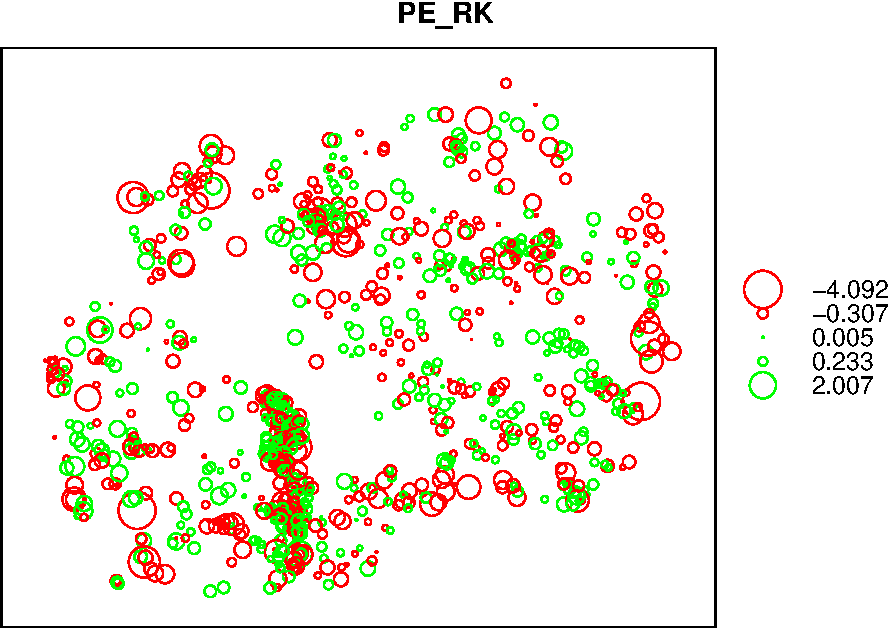
\includegraphics{SOCMapping_files/figure-latex/unnamed-chunk-88-1.pdf}
\caption{\label{fig:unnamed-chunk-88}Scatter plots of predicted against
observed values}
\end{figure}

\begin{Shaded}
\begin{Highlighting}[]
\KeywordTok{par}\NormalTok{(}\DataTypeTok{mfrow=}\KeywordTok{c}\NormalTok{(}\DecValTok{1}\NormalTok{,}\DecValTok{1}\NormalTok{))}
\end{Highlighting}
\end{Shaded}

\begin{Shaded}
\begin{Highlighting}[]
\CommentTok{# spatial bubbles for prediction errors}
\KeywordTok{bubble}\NormalTok{(dat[}\OperatorTok{!}\KeywordTok{is.na}\NormalTok{(dat}\OperatorTok{$}\NormalTok{PE_RK),], }\StringTok{"PE_RK"}\NormalTok{, }\DataTypeTok{pch =} \DecValTok{21}\NormalTok{, }
       \DataTypeTok{col=}\KeywordTok{c}\NormalTok{(}\StringTok{'red'}\NormalTok{, }\StringTok{'green'}\NormalTok{))}
\end{Highlighting}
\end{Shaded}

\begin{figure}
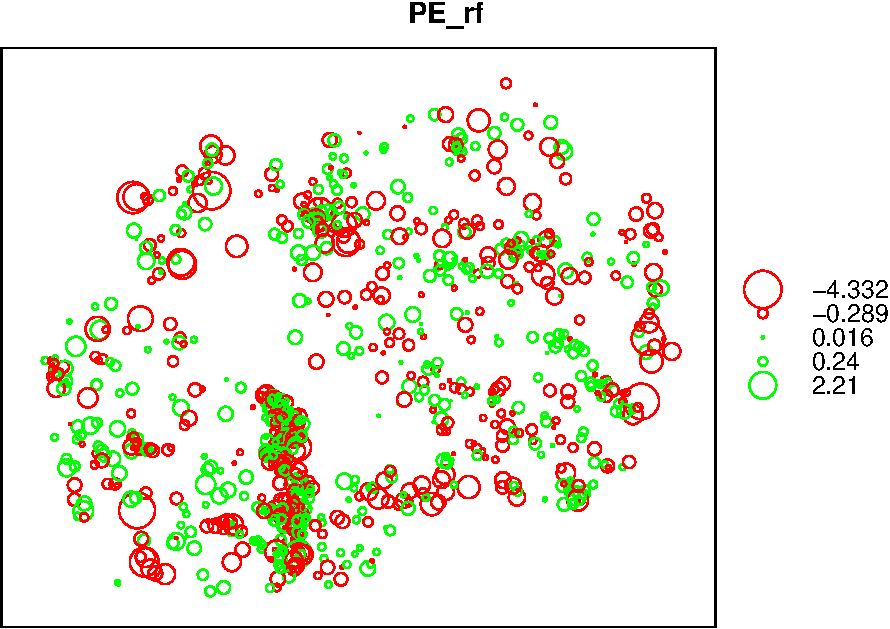
\includegraphics[width=0.6\linewidth]{SOCMapping_files/figure-latex/unnamed-chunk-89-1} \caption{Spatial bubble of the prediction errors for RK}\label{fig:unnamed-chunk-89}
\end{figure}

\begin{Shaded}
\begin{Highlighting}[]
\CommentTok{# spatial bubbles for prediction errors}
\KeywordTok{bubble}\NormalTok{(dat[}\OperatorTok{!}\KeywordTok{is.na}\NormalTok{(dat}\OperatorTok{$}\NormalTok{PE_rf),], }\StringTok{"PE_rf"}\NormalTok{, }\DataTypeTok{pch =} \DecValTok{21}\NormalTok{, }
       \DataTypeTok{col=}\KeywordTok{c}\NormalTok{(}\StringTok{'red'}\NormalTok{, }\StringTok{'green'}\NormalTok{))}
\end{Highlighting}
\end{Shaded}

\begin{figure}
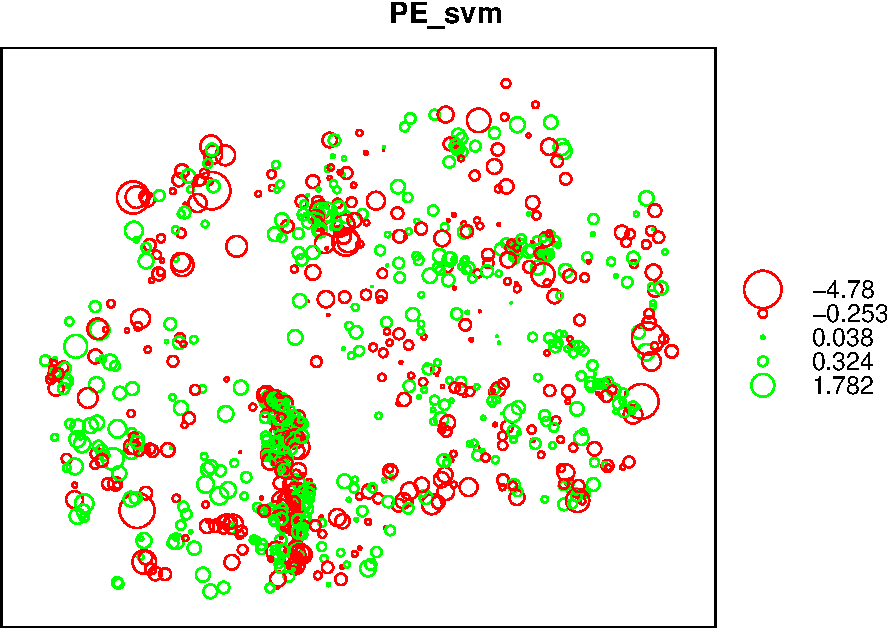
\includegraphics[width=0.6\linewidth]{SOCMapping_files/figure-latex/unnamed-chunk-90-1} \caption{Spatial bubble of the prediction errors for rf}\label{fig:unnamed-chunk-90}
\end{figure}

\begin{Shaded}
\begin{Highlighting}[]
\CommentTok{# spatial bubbles for prediction errors}
\KeywordTok{bubble}\NormalTok{(dat[}\OperatorTok{!}\KeywordTok{is.na}\NormalTok{(dat}\OperatorTok{$}\NormalTok{PE_svm),], }\StringTok{"PE_svm"}\NormalTok{, }\DataTypeTok{pch =} \DecValTok{21}\NormalTok{, }
       \DataTypeTok{col=}\KeywordTok{c}\NormalTok{(}\StringTok{'red'}\NormalTok{, }\StringTok{'green'}\NormalTok{))}
\end{Highlighting}
\end{Shaded}

\begin{figure}
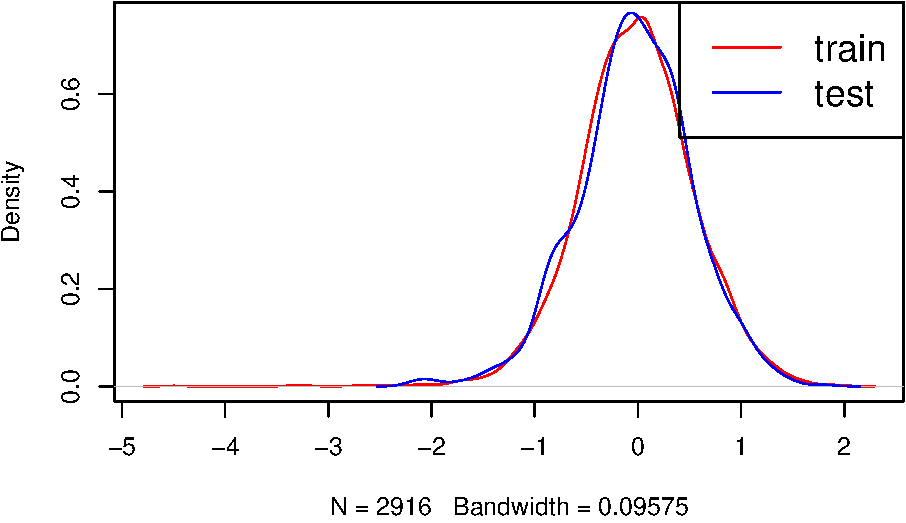
\includegraphics[width=0.6\linewidth]{SOCMapping_files/figure-latex/unnamed-chunk-91-1} \caption{Spatial bubble of the prediction errors for svm}\label{fig:unnamed-chunk-91}
\end{figure}

\hypertarget{dataSplit}{%
\subsection{Data-Splitting}\label{dataSplit}}

As explained before, many times for running validation analysis, we
split the data before fitting the models. In this section, we present
the code needed to achieve this using \textbf{caret} package.

\begin{Shaded}
\begin{Highlighting}[]
\KeywordTok{library}\NormalTok{(caret)}

\NormalTok{dat <-}\StringTok{ }\KeywordTok{read.csv}\NormalTok{(}\StringTok{"data/dataproc.csv"}\NormalTok{)}

\NormalTok{train.ind <-}\StringTok{ }\KeywordTok{createDataPartition}\NormalTok{(}\DecValTok{1}\OperatorTok{:}\KeywordTok{nrow}\NormalTok{(dat), }\DataTypeTok{p =} \FloatTok{.75}\NormalTok{, }\DataTypeTok{list =} \OtherTok{FALSE}\NormalTok{)}
\NormalTok{train <-}\StringTok{ }\NormalTok{dat[ train.ind,]}
\NormalTok{test  <-}\StringTok{ }\NormalTok{dat[}\OperatorTok{-}\NormalTok{train.ind,]}

\KeywordTok{plot}\NormalTok{(}\KeywordTok{density}\NormalTok{ (}\KeywordTok{log}\NormalTok{(train}\OperatorTok{$}\NormalTok{OCSKGM)), }\DataTypeTok{col=}\StringTok{'red'}\NormalTok{, }\DataTypeTok{main=}\StringTok{""}\NormalTok{)}
\KeywordTok{lines}\NormalTok{(}\KeywordTok{density}\NormalTok{(}\KeywordTok{log}\NormalTok{(test}\OperatorTok{$}\NormalTok{OCSKGM)), }\DataTypeTok{col=}\StringTok{'blue'}\NormalTok{)}
\KeywordTok{legend}\NormalTok{(}\StringTok{'topright'}\NormalTok{, }\DataTypeTok{legend=}\KeywordTok{c}\NormalTok{(}\StringTok{"train"}\NormalTok{, }\StringTok{"test"}\NormalTok{),}
      \DataTypeTok{col=}\KeywordTok{c}\NormalTok{(}\StringTok{"red"}\NormalTok{, }\StringTok{"blue"}\NormalTok{), }\DataTypeTok{lty=}\DecValTok{1}\NormalTok{, }\DataTypeTok{cex=}\FloatTok{1.5}\NormalTok{)}
\end{Highlighting}
\end{Shaded}

\begin{figure}
\centering
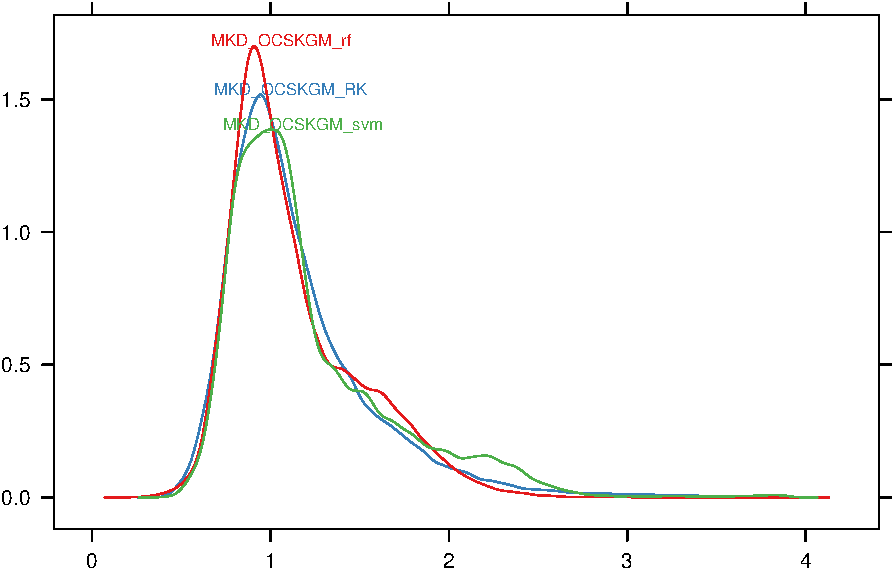
\includegraphics{SOCMapping_files/figure-latex/unnamed-chunk-93-1.pdf}
\caption{\label{fig:unnamed-chunk-93}Statistical distribution of train and
test datasets}
\end{figure}

\begin{Shaded}
\begin{Highlighting}[]
\KeywordTok{write.csv}\NormalTok{(train, }\DataTypeTok{file=}\StringTok{"data/dat_train.csv"}\NormalTok{, }\DataTypeTok{row.names =} \OtherTok{FALSE}\NormalTok{)}
\KeywordTok{write.csv}\NormalTok{(test, }\DataTypeTok{file=}\StringTok{"data/dat_test.csv"}\NormalTok{, }\DataTypeTok{row.names =} \OtherTok{FALSE}\NormalTok{)}
\end{Highlighting}
\end{Shaded}

\hypertarget{evaluation}{%
\chapter{Model Evaluation in Digital Soil Mapping}\label{evaluation}}

\emph{M Guevara \& GF Olmedo}

There are no best methods for statistical modeling and different
evaluation strategies should be considered in order to identify,
realistically, the overall modeling accuracy (\citet{ho2002simple};
\citet{qiao2015no}; \citet{soil-2017-40};
\citet{nussbaum2018evaluation}). This section is devoted to describe
quantitative methods for model evaluation applied to SOC mapping across
FYROM. Our objective is to provide a model evaluation example based on a
vector of observed SOC and a vector of modeled SOC estimates derived
from three different statistical methods (multiple linear
regression-kriging RK (Sect.\ref{RK}) random forests RF (Sect.\ref{rf}),
and support vector machines SVM (Sect.\ref{svm})). The model evaluation
methods presented here were adapted from the original work of Carslaw \&
Ropkins for air quality assessments and its R package openair
\citep{openair}.

We found in this package a very useful set of functions for model
evaluation metrics that are suitable (and we highly recommend) for
comparing digital soil maps derived from different prediction
algorithms. We will first analyze the simple correlation and major
differences of generated SOC maps by the three different methods. Then
for further analysis we will prepare a data frame containing the
observed and modeled vectors as well as the method column. Ideally the
observed vector should be derived from a completely independent SOC
dataset, as explained in the previous chapter. The cross validation
strategy and the repeated random split for training and testing the
models are other two alrernatives when no independent dataset is
available for validation purposes. However, we do not recommend to use
the same training dataset for performing the following analysis, since
the resulting `best method' could be the one that overfits the most.

\hypertarget{technical-steps---model-correlations-and-spatial-differences}{%
\section{Technical steps - Model correlations and spatial
differences}\label{technical-steps---model-correlations-and-spatial-differences}}

We will import the predicted maps and harmonize them in to the same
regular grid (\textasciitilde{}1x1km of spatial resolution). Then we
will plot the statistical distribution and the correlation between the
three different methods (RK, RF, SVM).

\begin{Shaded}
\begin{Highlighting}[]
\KeywordTok{library}\NormalTok{(raster)}
\NormalTok{RF<-}\KeywordTok{raster}\NormalTok{(}\StringTok{'results/MKD_OCSKGM_rf.tif'}\NormalTok{)}
\NormalTok{RK<-}\KeywordTok{raster}\NormalTok{(}\StringTok{'results/MKD_OCSKGM_RK.tif'}\NormalTok{)}
\NormalTok{SVM<-}\KeywordTok{raster}\NormalTok{(}\StringTok{'results/MKD_OCSKGM_svm.tif'}\NormalTok{)}
\CommentTok{#Note that RK has a different reference system }
\NormalTok{RK <-}\StringTok{ }\KeywordTok{projectRaster}\NormalTok{(RK, SVM)}
\NormalTok{models <-}\StringTok{ }\KeywordTok{stack}\NormalTok{(RK, RF, SVM)}

\KeywordTok{library}\NormalTok{(psych)}
\KeywordTok{pairs.panels}\NormalTok{(}\KeywordTok{na.omit}\NormalTok{(}\KeywordTok{as.data.frame}\NormalTok{(models)), }
             \DataTypeTok{method =} \StringTok{"pearson"}\NormalTok{, }\CommentTok{# correlation method}
             \DataTypeTok{hist.col =} \StringTok{"#00AFBB"}\NormalTok{,}
             \DataTypeTok{density =} \OtherTok{TRUE}\NormalTok{,  }\CommentTok{# show density plots}
             \DataTypeTok{ellipses =} \OtherTok{TRUE} \CommentTok{# show correlation ellipses}
\NormalTok{             )                     }
\end{Highlighting}
\end{Shaded}

\includegraphics[width=0.7\linewidth]{SOCMapping_files/figure-latex/unnamed-chunk-95-1}
Here we found that the higher correlation between predicted values was
between RK and SVM (0.86). We also found that the statistical
distribution of predicted values is quite similar between the three
methods and that the lowest correlation of predictions was found between
the two machine learning approaches (0.79, RF and SVM). We can in
addition overlap the probability distribution functions for the three
different methods to verify that their predictions are similar across
the full data distribution of values.

\begin{Shaded}
\begin{Highlighting}[]
\KeywordTok{library}\NormalTok{(rasterVis)}
\KeywordTok{densityplot}\NormalTok{(models)}
\end{Highlighting}
\end{Shaded}

\includegraphics{SOCMapping_files/figure-latex/unnamed-chunk-96-1.pdf}
Lets now take a look at the spatial differences. This step will allow to
identify the geographical areas within the prediction domain where model
predictions more agreee and disagree. To spatially compare model
predictions we will estimate the standard deviation and the differences
between the three SOC maps.

\begin{Shaded}
\begin{Highlighting}[]
\NormalTok{SD <-}\StringTok{ }\KeywordTok{calc}\NormalTok{(models , sd)}
\KeywordTok{library}\NormalTok{(mapview)}
\KeywordTok{mapview}\NormalTok{(SD)}
\end{Highlighting}
\end{Shaded}

The mapview command will plot the standard deviation map in a
\emph{.html} file. Note roughly how the hotspots (yellow to red colors)
of higher variance of predictions tend to be higher towards the west of
the country, whereas models tend to agree in their predictions across
the east side of the country. Note also that the variability although
noisy, it shows a general pattern, (e.g., from east to west), suggesting
that model agreement could be associated with specific land surface
characteristics. Now we will analyze specific differences between the
three models (RK vs RF, RK vs SVM, RF vs SVM).

\begin{Shaded}
\begin{Highlighting}[]
\NormalTok{RKRF  <-}\StringTok{ }\KeywordTok{calc}\NormalTok{(models[[}\KeywordTok{c}\NormalTok{(}\DecValTok{1}\NormalTok{,}\DecValTok{2}\NormalTok{)]], diff)}
\NormalTok{RKSVM <-}\StringTok{ }\KeywordTok{calc}\NormalTok{(models[[}\KeywordTok{c}\NormalTok{(}\DecValTok{1}\NormalTok{,}\DecValTok{3}\NormalTok{)]], diff)}
\NormalTok{RFSVM <-}\StringTok{ }\KeywordTok{calc}\NormalTok{(models[[}\KeywordTok{c}\NormalTok{(}\DecValTok{2}\NormalTok{,}\DecValTok{3}\NormalTok{)]], diff)}
\NormalTok{preds <-}\StringTok{ }\KeywordTok{stack}\NormalTok{(RKRF, RKSVM, RFSVM)}
\KeywordTok{names}\NormalTok{(preds) <-}\StringTok{ }\KeywordTok{c}\NormalTok{(}\StringTok{'RKvsRF'}\NormalTok{,}\StringTok{'RKvsSVM'}\NormalTok{,}\StringTok{'RFvsSVM'}\NormalTok{)}
\NormalTok{X <-}\StringTok{ }\KeywordTok{cellStats}\NormalTok{(preds, mean)}
\KeywordTok{levelplot}\NormalTok{(preds }\OperatorTok{-}\StringTok{ }\NormalTok{X, }\DataTypeTok{at=}\KeywordTok{seq}\NormalTok{(}\OperatorTok{-}\FloatTok{0.5}\NormalTok{,}\FloatTok{0.5}\NormalTok{, }\DataTypeTok{length.out=}\DecValTok{10}\NormalTok{), }\DataTypeTok{par.settings =}\NormalTok{ RdBuTheme)}
\end{Highlighting}
\end{Shaded}

\includegraphics{SOCMapping_files/figure-latex/unnamed-chunk-98-1.pdf}
Note how the spatial differences of the predicted SOC values have
similar patterns, but the difference between RK and RF semms to be less
sharp than the differences of SVM with the other two methods. Note that
we use the levelplot function to generate a better visualization (from
red-to-white-to-blue) of the main effects of differences (e.g., if they
are positive or negative), but we could also use the mapview function to
analyze these maps in a more interactive fashion. The variance of
predictions derived from different models can be used as a proxy of
model uncertainty and provides valuable information to consider in
further applications of SOC maps (e.g., modeling crop production or
quantifying SOC stocks).

\hypertarget{technical-steps---model-evaluation}{%
\section{Technical steps - Model
evaluation}\label{technical-steps---model-evaluation}}

To compare the performance of the three models, we will compare the
observed values used and the predicted values for the the validation
points. We have to load the validation dataset and the prediction result
of the 3 models. The table containing these values was prepared in
Section \ref{TS:validation}.

\begin{Shaded}
\begin{Highlighting}[]
\NormalTok{dat <-}\StringTok{ }\KeywordTok{read.csv}\NormalTok{(}\StringTok{"results/validation.csv"}\NormalTok{)}
\end{Highlighting}
\end{Shaded}

We will prepare a new table from this data that we are going to use for
model evaluation purposes. The new table should have the observed value,
the predicted value and the model.

\begin{Shaded}
\begin{Highlighting}[]
\CommentTok{# prepare 3 new data.frame with the observed, predicted and the model}
\NormalTok{modRK <-}\StringTok{ }\KeywordTok{data.frame}\NormalTok{(}\DataTypeTok{obs =}\NormalTok{ dat}\OperatorTok{$}\NormalTok{OCSKGM, }\DataTypeTok{mod =}\NormalTok{ dat}\OperatorTok{$}\NormalTok{MKD_OCSKGM_RK, }
                    \DataTypeTok{model =} \StringTok{"RK"}\NormalTok{)}

\NormalTok{modRF <-}\StringTok{ }\KeywordTok{data.frame}\NormalTok{(}\DataTypeTok{obs =}\NormalTok{ dat}\OperatorTok{$}\NormalTok{OCSKGM, }\DataTypeTok{mod =}\NormalTok{ dat}\OperatorTok{$}\NormalTok{MKD_OCSKGM_rf, }
                    \DataTypeTok{model =} \StringTok{"RF"}\NormalTok{)}

\NormalTok{modSVM <-}\StringTok{ }\KeywordTok{data.frame}\NormalTok{(}\DataTypeTok{obs =}\NormalTok{ dat}\OperatorTok{$}\NormalTok{OCSKGM, }\DataTypeTok{mod =}\NormalTok{ dat}\OperatorTok{$}\NormalTok{MKD_OCSKGM_svm, }
                     \DataTypeTok{model =} \StringTok{"SVM"}\NormalTok{)}

\CommentTok{# merge the 3 data.frames into one}
\NormalTok{modData <-}\StringTok{ }\KeywordTok{rbind}\NormalTok{(modRK, modRF, modSVM)}

\KeywordTok{summary}\NormalTok{(modData)}
\end{Highlighting}
\end{Shaded}

\begin{verbatim}
##       obs              mod         model    
##  Min.   :0.0111   Min.   :0.2980   RK :970  
##  1st Qu.:0.6681   1st Qu.:0.8196   RF :970  
##  Median :0.9518   Median :0.9589   SVM:970  
##  Mean   :1.1076   Mean   :1.0422            
##  3rd Qu.:1.3744   3rd Qu.:1.1507            
##  Max.   :6.1827   Max.   :3.3768            
##                   NA's   :34
\end{verbatim}

Now we will use the modStats function to calculate common numerical
model evaluation statistics which are described and mathematically
defined in the openair manual (\citet{carslaw2015openair}, Ch. 27, pp
231-233). These include:

\begin{itemize}
\tightlist
\item
  \(n\), the number of complete pairs of data.
\item
  \(FAC2\), fraction of predictions within a factor of two.
\item
  \(MB\), the mean bias.
\item
  \(MGE\), the mean gross error.
\item
  \(NMB\), the normalized mean bias.
\item
  \(NMGE\), the normalized mean gross error.
\item
  \(RMSE\), the root mean squared error.
\item
  \(r\), the Pearson correlation coefficient.
\item
  \(COE\), the Coefficient of Efficiency based on
  \citet{legates1999evaluating}, \citet{legates2013refined}. A perfect
  model has a \(COE\) = 1. A value of \(COE\) = 0.0 or negative implies
  no prediction capacity.
\item
  \(IOA\), the Index of Agreement based on \citet{willmott2012refined},
  which spans between -1 and 1 with values approaching +1 representing
  better model performance.
\end{itemize}

A perfect model would have a \(FAC24\), \(r\), \(COE\) and \(IOA\)
\textasciitilde{} 1.0, while all the others \textasciitilde{} 0.
However, digital soil mappers should have in mind that there is no such
thing as a perfect model on digital SOC mapping for large areas,
especially if we deal with sparse data from legacy soil profile or pit
observations usually collected over long periods of time. Depending on
the situation, some performance measures might be more appropriate than
others. Hence, there is not a single best measure, and it is necessary
to use a combination of the performance measures \citep{chang2004air}.

\begin{Shaded}
\begin{Highlighting}[]
\CommentTok{#Load the openair library}
\KeywordTok{library}\NormalTok{(openair)}

\NormalTok{modsts <-}\StringTok{ }\KeywordTok{modStats}\NormalTok{(modData,}\DataTypeTok{obs =} \StringTok{"obs"}\NormalTok{, }\DataTypeTok{mod =} \StringTok{"mod"}\NormalTok{, }\DataTypeTok{type =} \StringTok{"model"}\NormalTok{)}
\end{Highlighting}
\end{Shaded}

\begin{table}

\caption{\label{tab:modsts}Summary of Different Model Evaluation Statistics for the 3 Models Compared}
\centering
\begin{tabular}[t]{lrrrrrrrrr}
\toprule
model & FAC2 & MB & MGE & NMB & NMGE & RMSE & r & COE & IOA\\
\midrule
RK & 0.89 & -0.08 & 0.36 & -0.07 & 0.32 & 0.54 & 0.63 & 0.25 & 0.63\\
RF & 0.88 & -0.08 & 0.37 & -0.07 & 0.33 & 0.56 & 0.59 & 0.23 & 0.62\\
SVM & 0.86 & -0.03 & 0.39 & -0.02 & 0.36 & 0.58 & 0.53 & 0.18 & 0.59\\
\bottomrule
\end{tabular}
\end{table}

From our SOC mapping example across FYROM, the three models generate
similar results. The FAC2 is over to 0.8 in all cases, being RK the one
closer to 1. MB and NMB suggest that all the model's tent to
underestimate SOC because they are negative. SVM tend to underestimate
less than RK and RF. The MGE, NMGE, and RMSE suggest however that SVM is
generating the larger error rate and by the values of r COE and IOA, we
could say that given available SOC data across FYROM, the RK method
improves the predictive capacity of RF and SVM.

The aforementioned conclusion can be verified by plotting a Taylor
Diagram (Fig. \ref{fig:taylor}), which summarizes multiple aspects of
model performance, such as the agreement and variance between observed
and predicted values \citep{taylor2001summarizing}. Recent reports show
that the integration of simple validation metrics (e.g., the rmse
correlation ratio) allows to extract information about modeling
performance that could not be obtained by analyzing the validation
metrics independently, such as the agreement between explained variance
and bias (\citet{soil-2017-40}; \citet{nussbaum2018evaluation}). Taylor
Diagrams interpteration rely on the relationships between explained
variance and bias (from observed and modeled data). Note from our Taylor
Diagram that the RK method is closer to the observed value, followed by
RF. Although, no significant difference was evident between the three
implemented algorithms.

\begin{Shaded}
\begin{Highlighting}[]
\KeywordTok{TaylorDiagram}\NormalTok{(modData, }\DataTypeTok{obs =} \StringTok{"obs"}\NormalTok{, }\DataTypeTok{mod =} \StringTok{"mod"}\NormalTok{, }\DataTypeTok{group =} \StringTok{"model"}\NormalTok{,}
\DataTypeTok{cols =} \KeywordTok{c}\NormalTok{(}\StringTok{"orange"}\NormalTok{, }\StringTok{"red"}\NormalTok{,}\StringTok{"blue"}\NormalTok{), }\DataTypeTok{cor.col=}\StringTok{'brown'}\NormalTok{,}\DataTypeTok{rms.col=}\StringTok{'black'}\NormalTok{)}
\end{Highlighting}
\end{Shaded}

\begin{figure}
\centering
\includegraphics{SOCMapping_files/figure-latex/taylor-1.pdf}
\caption{\label{fig:taylor}Taylor diagram used in the evaluation of the 3
digital soil mapping models}
\end{figure}

However, we need also to check that the effectiveness of RK remains
across all the full distribution of SOC observed values. For doing this,
we can plot the conditional quantiles to verify the higher prediction
capacity of RK (Fig. \ref{fig:condquant}).

\begin{Shaded}
\begin{Highlighting}[]
\KeywordTok{conditionalQuantile}\NormalTok{(modData,}\DataTypeTok{obs =} \StringTok{"obs"}\NormalTok{, }\DataTypeTok{mod =} \StringTok{"mod"}\NormalTok{, }\DataTypeTok{type =} \StringTok{"model"}\NormalTok{)}
\end{Highlighting}
\end{Shaded}

\begin{figure}
\centering
\includegraphics{SOCMapping_files/figure-latex/condquant-1.pdf}
\caption{\label{fig:condquant}Effectiveness of the different digital soil
mapping models across the full distribution of SOC observed values}
\end{figure}

The blue line shows the results for a perfect model. In this case, the
observations cover a range from 0 to 6 kg.m-2. Interestingly, the
maximum predicted value is in all cases less than 3 kg.m-2, which is
consistent with the MB and NMB previous results. The red line shows the
median value of the predictions. Note that the median of predictions
across the larger SOC values seems to have more variability across SVM
and RK compared with RF, which tends to be conservative across the third
quantile of data distribution. The shading shows the predicted quantile
intervals (i.e.~the 25/75th and the10/90th). A perfect model (blue line)
would have a very narrow spread \citep{openair}. The histograms show the
counts of observed (gray) and predicted values (blue). While RF shows
more conservative results across the higher SOC values (e.g., over the
4th), SVM had the lowest model performance based these metrics. SVM was
also the method showing higher spatail differences compared with RF and
RK.

We conclude, for this specific example, that RK showed the best
performance based on the implemented evaluation metrics. Therefore RK is
a suitable method predicting SOC values across Macedonia, although other
methods generate similar results, we propose that, given available data,
RK could be also easier to interpret, because it provides the means to
identify the main effects and coefficients of the relationships across
the covariate space and the response variable. Beyond model evaluation,
the spatial combination of different modeling approaches (e.g., by the
means of the ensemble learning theory) should also be considered in
order to maximize the accuracy of results.

Finally, we want to highlight that Integrating different statistical
methods and visualization tools, such as those provided by the openair
package of R \citep{openair} will enhance our capacity to identify the
best modeling approaches and a combination of SOC prediction factors
given a specific dataset. Model evaluation benefits our understanding of
the circumstances why each modeling approach will generate different
results, which is a first step towards reducing uncertainty while
increasing the spatial resolution and accuracy of predictions, the
eternal digital soil mapping problem.

\hypertarget{uncertainty}{%
\chapter{Uncertainty}\label{uncertainty}}

\emph{GBM Heuvelink}

Soil mapping involves making predictions at locations where no soil
measurements were taken. This inevitably leads to prediction errors
because soil spatial variation is complex and cannot be modeled
perfectly. It also implies that we are uncertain about the true soil
class or true soil property at prediction locations. We only have the
predictions, which differ from the true values in an unpredictable way,
and hence we are uncertain about the true value. In fact, we may even be
uncertain about the soil at the measurement locations because no
measurement method is perfect and uncertainty also arises from
measurement errors.

This chapter describes how uncertainty may be characterized by
probability distributions. It also explains how the parameters of these
distributions may be derived, leading to quantification of uncertainty.
We will see that this can become quite complex, because soil properties
vary in space and are often cross-correlated, which the uncertainty
model must take into account. A further complication is that there are
many different sources of uncertainty. In some cases, it may be too
difficult to arrive at a spatially explicit characterization of
uncertainty, and in such case, statistical validation may be used to
derive summary measures of the accuracy of soil maps. We begin this
chapter with a description of uncertainty sources.

\hypertarget{sourcesuncert}{%
\section{Sources of Uncertainty}\label{sourcesuncert}}

Consider a case in which soil samples were taken from a large number of
measurement locations in a study area, taken to the laboratory and
analyzed for various soil properties. Let us further assume that the
measurement locations were indicated on a topographic map and that the
soil was also classified at each measurement location. Next, the soil
property and soil type observations were used to create maps of soil
properties and soil type using digital soil mapping techniques. These
techniques not only make use of the soil observations but also benefit
from maps of environmental variables that are correlated with the soil,
and hence help explain the soil spatial variation. Which sources of
uncertainty contribute to uncertainty about the final soil maps? We
distinguish four main categories.

\hypertarget{attribute-uncertainty-of-soil-measurements}{%
\subsection{Attribute Uncertainty of Soil
Measurements}\label{attribute-uncertainty-of-soil-measurements}}

Soil measurements suffer from measurement errors in the field and
laboratory. Perhaps the soil was not sampled at the right depth, perhaps
the organic layer was not removed completely before collecting soil
material, or perhaps by accident bags were interchanged or numbered
wrongly. Field estimates of soil type and soil properties are also not
error-free, especially when estimation is difficult, such as estimation
of SOC content or texture. Field estimates may also be subjective
because soil scientists may be trained differently and so there may be
systematic differences between their field estimates of soil properties.
Similarly, it is also not uncommon for soil scientists to disagree about
the soil type when classifying a soil in the field.

Laboratory analysis adds error too. Soil samples may not be perfectly
mixed prior to taking a much smaller subsample that is actually
measured; instruments have limited precision and may have systematic
errors, climate conditions in the lab vary, and there can be differences
between procedures used by laboratory personnel. Differences between
laboratories are even bigger and may be of the same order of magnitude
as the soil variation itself. It is strongly advised to always take
sufficient duplicates and randomize the order in which soil samples are
analyzed in the laboratory. This allows quantifying the combined field
and laboratory measurement errors.

\hypertarget{positional-uncertainty-of-soil-measurements}{%
\subsection{Positional Uncertainty of Soil
Measurements}\label{positional-uncertainty-of-soil-measurements}}

When collecting soil data in the field we would generally note the
geographic coordinates of the measurement locations. Nowadays this is
easy with GPS instruments and depending on the device, modest to high
positional accuracy can be achieved. But it may still be too large to be
negligible. For instance, consider the case where the soil data are used
to train a digital soil mapping model that predicts soil properties from
covariates. Let these covariates be available at high spatial resolution
and have substantial fine-scale spatial variation. Then it is clear that
positional uncertainty in the soil measurements may link these
measurements to the wrong covariates, which will weaken the strength of
the relationship between the soil variable and covariates and
deteriorate the quality of the final soil map.

Many soil legacy data suffer from large positional uncertainty.
Locations may only be traced from vague descriptions such as ``near
village A'' or ``east of the road from B to C''. In such case,
researchers should consider whether using such data for calibration of a
DSM model and for spatial prediction using the calibrated DSM model is
wise. It may do more harm than good. This depends on the specific DSM
model used and the degree of spatial variation of the covariates. It
also depends on the degree of spatial variation of the soil property
itself. If it has negligible fine-scale spatial variation and hence has
similar values at the registered and actual geographic location, then
little harm is done. For instance, in the Sahara desert many soil
properties will show little spatial variation over distances of hundreds
or perhaps thousands of meters, so in such case, poor geographic
positional accuracy will not seriously affect DSM predictions.

\hypertarget{uncertainty-in-covariates}{%
\subsection{Uncertainty in Covariates}\label{uncertainty-in-covariates}}

Maps of covariates that are used in DSM can also suffer from errors and
uncertainties. For instance, a Digital Elevation Model (DEM) is a major
source of geomorphological covariates but DEMs are only approximations
of the real elevation. DEM errors will propagate and cause uncertainty
in geomorphological properties such as slope, aspect and topographic
wetness index. As a result, the DSM model must be trained on covariate
data that are merely approximations of the intended covariates, which
will generally lead to weakened relationships and larger DSM prediction
errors. Land cover is another example; soil properties may be strongly
influenced by land cover, but such relationship may come out quite weak
if the DSM model is trained with a land cover map that represents land
cover wrongly for a large part of the study area.

Covariates also come in a specific spatial resolution which may be quite
coarse in specific cases. In order to use the covariate in a fine-scale
DSM model, the coarse-scale grid cell value will be copied to all
fine-scale grid cells contained in it, but clearly, fine-scale spatial
variation implies that uncertainties will be introduced. A possible
solution might be to smooth the coarse-scale covariate prior to entering
it to DSM calibration but clearly, this will not remedy all problems.

Uncertainty in covariates leads to weaker DSM models, but this weakening
is not hidden to the developer because the deterioration of predictive
power is implicitly included in the DSM model. For instance, the amount
of variance explained by a DSM model that uses the true land cover as
measured on sampling sites may be much higher than that of a model that
uses a land cover map. Users may then be tempted to calibrate the DSM
model with the true land cover data, but if they next apply that model
using the land cover map to predict the soil at non-measurement
locations they would systematically underestimate the uncertainty of the
resulting map.

\hypertarget{uncertainty-in-models-predicting-soil-properties-from-covariates-and-soil-point-data}{%
\subsection{Uncertainty in Models Predicting Soil Properties From
Covariates and Soil Point
Data}\label{uncertainty-in-models-predicting-soil-properties-from-covariates-and-soil-point-data}}

Even if the soil point data and covariate data were error-free, the
resulting DSM predictions would still deviate from the true soil
properties. This is because the DSM model itself also introduces
uncertainties. Models are merely simplified representations of the real
world. The real world is too complex and approximations are needed. For
instance, even though we know that physical, chemical and biological
processes determine the soil as given by the state equation of soil
formation \(soil\) = \(f\)(\(cl\), \(o\), \(r\), \(p\), \(t\)), the
function \(f\) is too complex to be fully understood and implemented in
a computer model. Instead, we use crude approximations such as multiple
linear regression and machine-learning algorithms. These empirical
models have the additional burden that extrapolation beyond conditions
represented by the calibration data is difficult and risky. For
extrapolation purposes, it is advised to use DSM models that better
represent the mechanisms behind soil formation, but again it is
practically impossible to build mechanistic models that represent the
real world perfectly. This is not only because we may not understand all
processes and their interactions well, but also because dynamic
mechanistic models need much information, such as the initial state,
boundary conditions, and driving forces. Such detailed information is
generally lacking.

Model uncertainty is generally subdivided into model parameter
uncertainty and model structural uncertainty. The first can be reduced
by using models with fewer parameters or by using a larger calibration
data set. The latter can be reduced by using a more complex model, but
this will only work if there are enough data to calibrate such model.
Thus, in general, a compromise has to be sought by choosing a level of
model complexity that matches the amount of information available.

\hypertarget{uncertainty-and-spatial-data-quality}{%
\section{Uncertainty and Spatial Data
Quality}\label{uncertainty-and-spatial-data-quality}}

Research into spatial accuracy in Geographic Information Science has
listed five main elements of spatial data quality: * lineage *
positional accuracy * attribute accuracy * logical consistency *
completeness

We have already discussed positional and attribute accuracy. Lineage
refers to documenting the original sources for the data and the
processing steps. This is strongly related to the principle of
reproducible research. Logical consistency addresses whether there are
any contradictory relationships in the database. For instance, it checks
whether all data have the same geographic projection and that
measurement units are consistent. Completeness refers to whether there
are any missing data. For instance, covariate maps must cover the entire
study area if they are to be used as explanatory variables in a DSM
model. Soil profile data need not capture all relevant soil properties
and tend to have fewer soil measurements at greater depths.

In summary, there are many sources of uncertainty that affect the
quality of DSM products. This section has reviewed these sources but was
purposely descriptive. The next section selects a few major uncertainty
sources and works out quantitatively how these cause uncertainty in the
resulting soil map. Perhaps it is useful to mention that focussing
attention on errors and uncertainties may give the wrong impression that
soil maps are generally inaccurate and of poor quality. This is not the
message that we wish to convey here. But producers and users of soil
maps should be aware of the sources of uncertainty and should ideally
identify how these uncertainties affect the final product. Thus,
quantification of the uncertainty in DSM maps, be it through explicit
modeling or independent validation is important.

\hypertarget{quantifying-prediction-uncertainty}{%
\section{Quantifying Prediction
Uncertainty}\label{quantifying-prediction-uncertainty}}

Uncertainties in soil measurements, covariates and DSM models propagate
to resulting soil maps. The uncertainty propagation can fairly easily be
traced provided that the uncertainty sources are characterized
adequately. The most appropriate way of doing that is by making use of
statistics and probability distributions. This section also takes that
approach and starts by providing a brief overview of probability
distributions and how these may be used to represent uncertainty. Next,
it analyses how the four sources of uncertainty distinguished in Section
5.1 lead to uncertainty in soil maps produced using DSM.

\hypertarget{uncertainty-characterised-by-probability-distributions}{%
\subsection{Uncertainty Characterised by Probability
Distributions}\label{uncertainty-characterised-by-probability-distributions}}

If we are uncertain about the value of a soil property at some location
and depth this means that we cannot identify one single, true value for
that soil property
(\cite{goovaerts2001geostatistical, arrouays_uncertainty_2014}).
Instead, we may be able to provide a list of all possible values for it
and attach a probability to each. In other words, we represent the true
but unknown soil property by a probability distribution. For instance,
suppose that we estimate the sand content of a soil sample in the field
as \(35\%\), while recognizing that a field estimate is quite crude and
that the true sand content may very well be less or more than the
estimated \(35\%\). We might be confident that the estimation error is
unlikely to be greater than \(8\%\), and hence it would be reasonable to
represent the sand content by a normal distribution with a mean of
\(35\%\) and a standard deviation of \(4\%\). For the normal
distribution, \(95\%\) of the probability mass lies within two standard
deviations from the mean, so we would claim that there is a \(5\%\)
probability that the sand content is smaller than \(27\%\) or greater
than \(43\%\).

In the example above we had chosen the normal distribution because it is
the most common probability distribution but we might as well have used
a different distribution, such as the uniform or lognormal distribution.
Indeed many soil properties, such as soil nutrient concentrations are
better described by lognormal distributions, because values below zero
cannot occur and because very high positive values (i.e.~outliers) are
not unlikely. For instance, we may estimate the organic carbon
concentration (OC) of a soil sample as \(1.2\%\) and identify with it an
asymmetric \(95\%\) credibility interval ranging from \(0.8\%\) to
\(2.5\%\). In general, statistical modeling is easier if the variables
under study can be described by normal distributions. This explains why
we usually apply a transformation to skewed variables prior to
statistical modeling. For instance, when building a DSM model of OC, it
may be wise to develop such model for the logarithm of OC and do a
back-transform on the DSM predictions.

There are many different soil properties that in addition vary in space
and possibly time. Thus, the characterization of uncertainty about soil
properties needs to be extended and include cross- and space-time
correlations. It is beyond the scope of this chapter to explain this in
detail, for this we refer to standard textbooks such as
\cite{goovaerts1997geostatistics} and \cite{webster_2007}. If we assume
a joint normal distribution, then a vector of soil properties (be it
different soil properties or the same soil property at multiple
locations, depths or times) \(Z\) is fully characterized by the vector
of means \(m\) and variance-covariance matrix \(C\). Figure
\ref{fig:pairedsoils} shows three examples of 500 paired soil property
values that were simulated from different bivariate normal
distributions. The left panel shows an uncorrelated case with equal
standard deviations for both properties. The centre and right panels
show a case where soil property 2 has a greater standard deviation than
soil property 1. The difference between these two cases is that the
centre panel has a zero correlation between the two soil properties
while it is positive in the right panel.

\begin{figure}

{\centering \includegraphics[width=0.8\linewidth]{images/pairedsoilpropierties} 

}

\caption{Scatter plots of 500 paired soil property values drawn from a two-dimensional normal distribution}\label{fig:pairedsoils}
\end{figure}

\hypertarget{propagation-of-model-uncertainty}{%
\subsection{Propagation of Model
Uncertainty}\label{propagation-of-model-uncertainty}}

Now that we have clarified how uncertainty in soil properties may be
characterized by probability distributions, let us consider what these
distributions look like in DSM and how these are influenced by the
uncertainty sources described in Section \ref{sourcesuncert}. We begin
with uncertainty source 4, uncertainty in DSM models. We noted before
that uncertainty in DSM models may be separated in model parameter and
model structural uncertainty. A typical example of this is a multiple
linear regression model:

\begin{equation}
\label{eq:DSM model}
Z(s) = \beta_0 + \beta_1  \cdot X_1 (s) + \beta_2 \cdot X_2 (s) + \varepsilon(s)
\end{equation}

Note that here for simplicity we assumed two environmental covariates
\({X1}\) and \({X_2}\) while in practice we are likely to use many more.
Parameter uncertainty of this model occurs because the parameters
\({\beta_0}\) , \({\beta_1}\) and \({\beta_2}\) are merely estimated
using calibration data. Under the assumptions made by the linear
regression model, these estimation errors are normally distributed and
have zero mean, while their standard deviations and cross-correlations
can also be computed (e.g.~Snedecor and Cochran 1989, Section 17.5). The
standard deviations become smaller as the size of the calibration
dataset increases. Both the standard deviations and cross-correlations
are standard output of statistical software packages. Thus, we could
sample from the joint distribution of the parameter estimation errors in
a similar way as displayed in Figure \ref{fig:pairedsoils}.

The model structural uncertainty associated with the multiple linear
regression model Eq. \ref{eq:DSM model} is represented by the stochastic
residual \({\varepsilon}\). It too is normally distributed and has zero
mean, while its standard deviation depends on the (spatial) variation of
the soil property \(Z\) and the strength of the relationship between
\(Z\) and the covariates \({X_1}\) and \({X_2}\). If the covariates
explain a great deal of the variation of the soil property then the
standard deviation of the residual will be much smaller than that of the
soil property, as expressed by the goodness-of-fit characteristic
\({R^2}\), also termed `amount of variance explained'. It will be close
to 1 in case of a strong linear relationship between soil property and
covariates. In that case, the standard deviation of the stochastic
residual will be much smaller than that of the soil property, because a
large part of the variation is explained by the model. If the covariates
bear no linear relationship with the soil property (i.e., \({R^2}\) =
0), the stochastic residual will have the same standard deviation as the
soil property.

Since the joint probability distributions of the parameter estimation
errors and the stochastic residual can analytically be computed and are
routinely provided by statistical software, it is not difficult to
analyse how these uncertainties propagate through the DSM model Eq.
\ref{eq:DSM model}. This can be done analytically, because Eq.
\ref{eq:DSM model} is linear in the stochastic arguments (note that the
covariates are treated known and deterministic). If we predict the soil
property \(Z\) at a prediction location \({s_0}\) using the calibrated
regression model as:

\begin{equation}
\label{eq:cal regmodel}
\hat{Z}(s_0) = \hat{\beta}_0 + \hat{\beta}_1  \cdot X_1 (s_0) +  \hat{\beta}_2 \cdot X_2 (s_0)
\end{equation}

then the prediction error will be normally distributed with zero mean
and variance (i.e., the square of the standard deviation) given by:

\begin{equation}
\begin{aligned}
\label{eq:pred err}
Var(\hat{Z}(s_0)) - Z(s_0)) = & \ Var(\hat{\beta}_0) + Var(\hat{\beta}_1)  \cdot X_1 (s_0)^2 +  Var(\hat{\beta}_2) \cdot X_2 (s_0)^2 + \\
                      & \ 2 Cov(\hat{\beta}_0,\hat{\beta}_1) \cdot  X_1 (s_0) + 2 Cov(\hat{\beta}_0,\hat{\beta}_2) \cdot X_2 (s_0) + \\
                      & \ 2 Cov(\hat{\beta}_1,\hat{\beta}_2) \cdot  X_1 (s_0) \cdot  X_2 (s_0) + Var(\varepsilon(s_0))
\end{aligned}
\end{equation}

This is a complicated expression but all entries are known and hence it
can be easily calculated.

In many DSM applications, an additional step will be included that makes
use of the fact that the stochastic residual \({\varepsilon}\) in Eq.
\ref{eq:DSM model} is spatially autocorrelated, as characterized by a
semivariogram. If this is the case the residual spatial correlation can
be exploited by incorporating a kriging step \citep{hengl2004generic}.
Kriging has been explained in Chapter 6, where it was also explained
that the uncertainty in the predictions is quantified by the kriging
variance. We will not repeat the theory here, but simply note that the
kriging variance computes the prediction error variance just as was done
in Eq. \ref{eq:pred err}, but that in case of kriging the
\({Var(\varepsilon(s_0)))}\) term in Eq. \ref{eq:pred err} is replaced
by a smaller term, because kriging benefits from residual spatial
correlation. In fact, in case of a pure nugget variogram, the kriging
variance would be identical to Eq. \ref{eq:pred err}, because in such
case there is no spatial autocorrelation that one can benefit from. Note
also that here we refer to Kriging with External Drift because we
included a non-constant mean (i.e., covariates \({X1}\) and \({X_2}\)).
If no covariates were included Eq. \ref{eq:pred err} would simplify
dramatically leaving only uncertainty in the estimated (constant) mean
and the stochastic residual. This might then be compared with the
ordinary kriging variance.

So far we considered uncertainty in DSM models that are linear in the
covariates and that represent the model structural uncertainty by an
additive stochastic term. This was relatively easy because tracing how
uncertainty in model parameters and model structure propagate to the
model output could be done analytically. However, using linear models
also poses serious restrictions. The relationship between soil
properties and covariates are typically not linear but much more
complex. This has led to the development and use of complex non-linear
DSM models, such as regression trees, artificial neural networks,
support vector machines and random forests approaches, all summarised
under the term `machine learning' (e.g. \cite{hengl2015mapping}). These
more complex models typically yield more accurate soil predictions but
quantification of the associated uncertainty is more difficult. In most
cases, one resorts to validation and cross-validation statistics that
summarise the prediction accuracy over the entire study area. How this
is done will be explained in detail in 7.3. Such summary validation
measures are very valuable but are no substitute for spatially explicit
uncertainties such as the kriging variance and the prediction error
variance presented in Eq. \ref{eq:pred err}. Research into
quantification of location-specific uncertainties when using machine
learning algorithms is therefore important. However, it is beyond the
scope of this chapter to review this area of ongoing research. One
particular approach makes use of quantile regression forests. We refer
to \cite{meinshausen2006quantile} for a general text and to
\cite{vaysse2017using} for a DSM application of this promising, albeit
computationally challenging approach.

\hypertarget{propagation-of-attribute-positional-and-covariate-uncertainty}{%
\subsection{Propagation of Attribute, Positional and Covariate
Uncertainty}\label{propagation-of-attribute-positional-and-covariate-uncertainty}}

In Section 7.1 we noted that next to uncertainties in model parameters
and model structure there may also be uncertainties in the attribute
values and positions of the soil point data and in the covariates. These
sources of uncertainty will also affect the outcome of DSM model
predictions.

Uncertainties in soil attribute values effectively mean that the DSM
model is calibrated with error-contaminated observations of the
dependent variable. Let us consider the multiple linear regression model
Eq. \ref{eq:DSM model} again. True values of the dependent variable Z
(i.e., the target soil property, such as pH, clay content or total
nitrogen concentration) are no longer for calibration of this model.
Instead, we must make do with measurements \(Y\) of \(Z\):

\begin{equation}
Y(s_i) = Z(s_i) + \delta(s_i), \quad i = 1 \dots n
\end{equation}

where \(n\) is the number of measurement locations and \({\delta(s_i)}\)
is a random variable representing measurement error. It is custom to
assume that all \({\delta(s_i)}\) are normally distributed, have zero
mean and are mutually independent, although these assumptions are not
strictly necessary. Their standard deviations may vary between cases and
depend on the accuracy and precision of the measurement method. For
instance, field estimates tend to be more uncertain than laboratory
measurements and so the corresponding measurement errors will have a
larger standard deviation. The consequence of the presence of
measurement errors is that the estimates of the model parameters will be
more uncertain. This is no surprise because the calibration data are of
poorer quality. The prediction error variance will be greater too, for
the same reason. If spatial correlation of the model residual
\({\varepsilon}\) is included and an extension to Kriging with External
Drift is made, uncertainty due to measurement errors is further
increased because the conditioning of predictions to observations cannot
benefit as much as when the observations were error-free. For
mathematical details we refer to \cite{cressie1993statistics}. Finally,
we should also note that if different observations have different
degrees of measurement error, then this will influence the weights that
each measurement gets in calibration and prediction. Measurements with
larger measurement errors get smaller weights. This is automatically
incorporated in multiple linear regression and Kriging with External
Drift, but how this can be incorporated in machine-learning approaches
is less clear.

Positional uncertainty of soil point observations will also deteriorate
the quality of the predictions of calibrated DSM models. However, it is
difficult to predict how much the prediction accuracy is affected. It
largely depends on the degree of fine-scale spatial variation of the
soil property and covariates. For instance, if both the soil property of
interest and the covariates are spatially smooth and hardly change over
distances within the range of spatial displacement due to positional
uncertainty, then little damage is afflicted by positional uncertainty.
But otherwise much harm can be done because the soil observations will
be paired with covariate values from displaced locations that can be
very different. So far, this interesting and important topic has
received only little attention in the DSM literature.
\cite{grimm2010uncertainty} and \cite{nelson2011error} are two examples
of studies that assessed the effect of positional error on the accuracy
of digital soil maps.

Finally, there are also uncertainties in covariates that affect the
accuracy of DSM predictions. In fact, these uncertainties are already
incorporated in the model structural uncertainty discussed before,
because offering covariates that are poor approximations of the true
soil forming factors will explain little of the spatial variation and
lead to low goodness-of-fit statistics. From a statistical point of
view, the covariates used in Eq. \ref{eq:DSM model} need not be the
`true' soil forming factors but could as well be proxies of those. This
does not harm the theory and quantification of the prediction error
variance such as through Eq. \ref{eq:pred err} in the multiple linear
regression case or using the kriging variance in a KED approach remain
perfectly valid. This does not mean that digital soil mappers should not
look for the most accurate and informative covariates because clearly
weak covariates lead to poor predictions of the soil (e.g.~Samuel Rosa
et al.~2015).

\hypertarget{data-sharing}{%
\chapter{Data Sharing}\label{data-sharing}}

\emph{T Hengl, L Poggio, E Ribeiro \& B Kempen}

This chapter reviews possibilities and ``good practices'' of exchanging
produced soil data. Once the analysis, spatial prediction and quality
control have been all completed, it is useful to follow some minimum
steps and export and prepare the data for distribution so that its
potential users can easily access it, use it, and make a correct
interpretation of data. We consider geo-publishing options for soil data
either based on using third-party web services or by using one's own
installation of the software. We put a clear focus on using the Open
Source software solutions: GDAL, R, GeoServer, OpenLayers and Leaflet,
and public domain data and metadata standards.

The authors have 15+ years of experience in producing, publishing and
sharing soil maps and have been involved in large soil mapping projects
where data volumes often exceed standard desktop GIS capacities. For
information on specific software please refer to the provided links.
Even more information on using GDAL and similar GIS tools through a
command line can be found via the Global Soil Information Facilities
tutorials of ISRIC at \url{http://gsif.isric.org}. The text is
illustrated with example scripts of the statistical software R in
combination with GDAL.

\hypertarget{export-formats}{%
\section{Export Formats}\label{export-formats}}

\hypertarget{type-of-soil-data-and-their-formatting}{%
\subsection{Type of Soil Data and Their
Formatting}\label{type-of-soil-data-and-their-formatting}}

Before we start reviewing soil data formats, it is useful to understand
which types of soil variables, soil maps, and soil DBs are most commonly
generated and used, and what are their specific advantages and
limitations. Soil science works with many variables common to ecology
and/or physical geography (e.g.~soil temperature), but it also works
with several variables specific to soil science only. Some soil
factor-type variables specific to soil science only are for example:

\begin{itemize}
\tightlist
\item
  Soil taxa or soil classes (this includes taxonomic systems and
  connected diagnostic soil properties and horizons).
\item
  Soil texture-class systems.
\item
  Soil color classification systems e.g.~Munsell color codes.
\item
  Soil drainage classes (hydrological classifications).
\item
  Soil diagnostic horizons.
\end{itemize}

Consider for example the following soil texture data:

\begin{Shaded}
\begin{Highlighting}[]
\KeywordTok{library}\NormalTok{(soiltexture)}
\NormalTok{tex <-}\StringTok{ }\KeywordTok{data.frame}\NormalTok{(}
  \DataTypeTok{CLAY =} \KeywordTok{c}\NormalTok{(}\DecValTok{05}\NormalTok{,}\DecValTok{60}\NormalTok{,}\DecValTok{15}\NormalTok{,}\DecValTok{05}\NormalTok{,}\DecValTok{25}\NormalTok{,}\DecValTok{05}\NormalTok{,}\DecValTok{25}\NormalTok{,}\DecValTok{45}\NormalTok{,}\DecValTok{65}\NormalTok{,}\DecValTok{75}\NormalTok{,}\DecValTok{13}\NormalTok{,}\DecValTok{47}\NormalTok{),}
  \DataTypeTok{SILT =} \KeywordTok{c}\NormalTok{(}\DecValTok{05}\NormalTok{,}\DecValTok{08}\NormalTok{,}\DecValTok{15}\NormalTok{,}\DecValTok{25}\NormalTok{,}\DecValTok{55}\NormalTok{,}\DecValTok{85}\NormalTok{,}\DecValTok{65}\NormalTok{,}\DecValTok{45}\NormalTok{,}\DecValTok{15}\NormalTok{,}\DecValTok{15}\NormalTok{,}\DecValTok{17}\NormalTok{,}\DecValTok{43}\NormalTok{),}
  \DataTypeTok{SAND =} \KeywordTok{c}\NormalTok{(}\DecValTok{90}\NormalTok{,}\DecValTok{32}\NormalTok{,}\DecValTok{70}\NormalTok{,}\DecValTok{70}\NormalTok{,}\DecValTok{20}\NormalTok{,}\DecValTok{10}\NormalTok{,}\DecValTok{10}\NormalTok{,}\DecValTok{10}\NormalTok{,}\DecValTok{20}\NormalTok{,}\DecValTok{10}\NormalTok{,}\DecValTok{70}\NormalTok{,}\DecValTok{10}\NormalTok{)}
\NormalTok{ )}
 
\KeywordTok{TT.plot}\NormalTok{(}\DataTypeTok{class.sys =} \StringTok{"USDA.TT"}\NormalTok{, }\DataTypeTok{tri.data =}\NormalTok{ tex, }\DataTypeTok{main =} \StringTok{""}\NormalTok{, }
        \DataTypeTok{cex.axis=}\NormalTok{.}\DecValTok{7}\NormalTok{, }\DataTypeTok{cex.lab=}\NormalTok{.}\DecValTok{7}\NormalTok{)}
\end{Highlighting}
\end{Shaded}

\begin{figure}
\centering
\includegraphics{images/Data_sharing_triangle.png}
\caption{Soil texture triangle plot. An example of soil science specific
data.}
\end{figure}

The way soil texture data is displayed and texture classes (SaLo, Lo, Sa
etc.) used in a texture triangle is specific to soil science. The way
this data is formatted and presented can be, likewise, specific to soil
science only.

Most of the soil data is in fact spatial. \textbf{``Spatial''} implies
that spatial (and temporal) reference is attached to each
measured/estimated value, i.e.~it is location specific. Spatio-temporal
references typically include for example:

\begin{itemize}
\tightlist
\item
  Geographic location in local or geographic coordinates (ideally
  longitude and latitude in the WGS84 coordinate system);
\item
  Depth interval expressed in cm from land surface (upper and lower
  depth);
\item
  Support size or referent soil volume (or voxel) i.e.~the horizontal
  sampling area multiplied by the thickness of the sampling block;
\item
  Temporal reference i.e.~begin and end date/time of the period of
  measurements/estimations.
\end{itemize}

Spatial data formats are used to represent spatial objects. This can be
\citep[neteler2013open]{bivand2013classes}:

\begin{itemize}
\tightlist
\item
  Points (2D or 3D): used to represent sampling locations, soil
  horizons, soil profiles etc.
\item
  Lines (2D): used to represent soil transects, streams, administrative
  boundaries etc.
\item
  Polygons (2D): used to represent soil mapping units and/or
  geomorphological units, landforms, administrative areas, farms, plot
  trials etc.
\item
  Grids or rasters (2D or 2.5D): used to represent soil spatial
  predictions (spatially complete) of soil properties and classes etc.
\item
  3D grids or Voxels: used to represent soil spatial predictions
  (spatially complete) of soil properties in 3D.
\end{itemize}

It is also important to be able to distinguish between sampled or
predicted soil data:

\begin{enumerate}
\def\labelenumi{\arabic{enumi}.}
\tightlist
\item
  Soil samples (usually points or transects) are spatially incomplete.
  They are used to generate spatial predictions.
\item
  Spatial predictions of soil variables (soil maps) are spatially
  complete. They are used for decision making and further modeling
  i.e.~they are used to construct a Soil Information System.
\end{enumerate}

\begin{figure}
\centering
\includegraphics{images/Data_sharing_soil_variables.png}
\caption{Some frequently required soil variables (sorted by number of
studies) based on the study by Keller et al. (2014). This list is
probably country/project specific but illustrates the differences
considering the interest in soil data.}
\end{figure}

A collection of spatially exhaustive soil grids of various soil
properties (physical and chemical soil properties, soil water, soil
classification etc) make a \textbf{Soil Information System} (SIS). SIS
are often complemented with soil sample data and serve both data
formats. A Soil Information System should preferably be a
\textbf{Database} (DB), so that users can access and query data using
some standard DB languages (for example SQL). Steps to export soil data
into a DB format are explained in later sections.

\hypertarget{general-gis-data-formats-vector-raster-table}{%
\subsection{General GIS Data Formats: Vector, Raster,
Table}\label{general-gis-data-formats-vector-raster-table}}

All soil data we produce through soil mapping can be in principle
distributed using one of the two basic GIS formats of data:

\begin{itemize}
\tightlist
\item
  Vector format: this format is often more suitable for exporting point,
  line, and polygon (areal) data,
\item
  Raster or gridded format: this format is often more suitable for
  exporting spatial predictions of soil variables.
\end{itemize}

Data in vector format can be converted to raster (see e.g.~rasterize
function in the raster R package ) and vice versa --- raster data can be
converted to vector formats. For example, rasters can be converted to
polygons (see e.g.~rast2vect function in the plotKML package ). If the
conversion is done carefully and if all the relations between scale and
pixel size have been considered (see \citet{hengl2006finding} for more
details), then information loss due to conversion from raster to vector
and vice versa should be minimal.

Both vector and raster GIS data can also be converted to tabular data
format. By converting a GIS layer to a table, spatial geometry and
spatial relations will be `stripped off', so that only limited spatial
analysis operations can be applied. To convert raster layers to tabular
data, consider using the \textbf{SpatialPixelsDataFrame-class} in the sp
package and/or the \textbf{RasterLayer-class} from the raster package in
combination with the rgdal package \citep{bivand2013classes}:

\begin{Shaded}
\begin{Highlighting}[]
\KeywordTok{library}\NormalTok{(rgdal)}
\KeywordTok{library}\NormalTok{(plotKML)}
\NormalTok{?readGDAL}
\NormalTok{spnad83 <-}\StringTok{ }\KeywordTok{readGDAL}\NormalTok{(}\KeywordTok{system.file}\NormalTok{(}\StringTok{"pictures/erdas_spnad83.tif"}\NormalTok{, }
                                \DataTypeTok{package =} \StringTok{"rgdal"}\NormalTok{)[}\DecValTok{1}\NormalTok{])}
\NormalTok{spnad83.tbl <-}\StringTok{ }\KeywordTok{as.data.frame}\NormalTok{(spnad83)}
\KeywordTok{str}\NormalTok{(spnad83.tbl)}
\end{Highlighting}
\end{Shaded}

where as.data.frame is a function converting a raster object to a table.
Note that the output table now contains coordinates for each cell
(center of the grid node), which is in fact memory inefficient as
coordinates are provided for each row in the table.

Likewise, to convert a vector layer to tabular formats one can use the
Simple Features functionality of the sf package . The SF standard is
widely implemented in spatial databases (PostGIS, ESRI ArcGIS) and forms
the vector data basis for libraries such as GDAL and web standards such
as GeoJSON (\url{http://geojson.org/}). To convert for example spatial
polygons layer to a tabular format we would use:

\begin{Shaded}
\begin{Highlighting}[]
\KeywordTok{library}\NormalTok{(sf); }\KeywordTok{library}\NormalTok{(plotKML)}
\KeywordTok{data}\NormalTok{(eberg_zones)}
\KeywordTok{class}\NormalTok{(eberg_zones)}
\NormalTok{eberg_zones.tbl <-}\StringTok{ }\KeywordTok{as}\NormalTok{(eberg_zones, }\StringTok{"sf"}\NormalTok{)}
\KeywordTok{str}\NormalTok{(eberg_zones.tbl)}
\end{Highlighting}
\end{Shaded}

Note that using spatial layers in simple tabular formats can be
cumbersome because many spatial relationships and properties are likely
lost (although these can be assigned reversibly). In addition, the size
of tabular objects is much bigger than if we use data in the original
GIS data formats, especially if those formats support compression. On
the other hand, having data in tabular format can be often the only way
to exchange the data from spatial to non-spatial databases or from
software without any data communication bridge. Also, tabular data is
human-readable which means that it can be opened in text editors,
spreadsheet programs or similar.

\hypertarget{recommended-gis-data-exchange-formats}{%
\subsection{Recommended GIS Data Exchange
Formats}\label{recommended-gis-data-exchange-formats}}

As a general recommendation producers of soil data should primarily look
at using the following data formats for exchanging soil data (points,
polygons, and rasters):

\begin{itemize}
\tightlist
\item
  GPKG (an Open Format for Geospatial Information):
  platform-independent, portable, self-describing, compact format for
  transferring geospatial information.
\item
  GeoTIFF (for rasters): a TIFF (image) file that allows embedding
  spatial reference information, metadata and color legends. It also
  supports internal compression algorithms and hierarchical indexing.
\end{itemize}

Both formats can be read easily in R or similar data processing
software. Vectors are also commonly exported and shared in ESRI
Shapefile (SHP) format. The advantage of GPKG format versus somewhat
more common ESRI SHP format is that GPKG files are basically a portable
database (SQLite container) so that the user does not have to import the
whole data into a program but also fetch parts of data by using SQL
queries and it can handle vector and raster data in it. The following
example demonstrates how to create a GPKG file and how to query it:

\begin{Shaded}
\begin{Highlighting}[]
\KeywordTok{library}\NormalTok{(RSQLite)}
\KeywordTok{data}\NormalTok{(eberg)}
\KeywordTok{coordinates}\NormalTok{(eberg) <-}\StringTok{ }\ErrorTok{~}\NormalTok{X}\OperatorTok{+}\NormalTok{Y}
\KeywordTok{proj4string}\NormalTok{(eberg) <-}\StringTok{ }\KeywordTok{CRS}\NormalTok{(}\StringTok{"+init=epsg:31467"}\NormalTok{)}
\KeywordTok{writeOGR}\NormalTok{(eberg, }\StringTok{"eberg.gpkg"}\NormalTok{, }\StringTok{"eberg"}\NormalTok{, }\StringTok{"GPKG"}\NormalTok{)}
\NormalTok{con <-}\StringTok{ }\KeywordTok{dbConnect}\NormalTok{(RSQLite}\OperatorTok{::}\KeywordTok{SQLite}\NormalTok{(), }\DataTypeTok{dbname =} \StringTok{"eberg.gpkg"}\NormalTok{)}
\NormalTok{df <-}\StringTok{ }\KeywordTok{dbGetQuery}\NormalTok{(con, }\StringTok{'select "soiltype" from eberg'}\NormalTok{)}
\KeywordTok{summary}\NormalTok{(}\KeywordTok{as.factor}\NormalTok{(df}\OperatorTok{$}\NormalTok{soiltype))}
\KeywordTok{dbGetQuery}\NormalTok{(con, }
           \StringTok{'select * from gpkg_spatial_ref_sys'}\NormalTok{)[}\DecValTok{3}\NormalTok{,}\StringTok{"description"}\NormalTok{]}
\end{Highlighting}
\end{Shaded}

Note that the RSQLite package is a generic package for connecting to
SQLite DBs. This means that GPKG files can be accessed and updated in
its native storage format without intermediate format translations. Just
putting a GPKG file on a server with read and execute access allows
users to connect and fetch data.

Alternatively, it is also a good idea to store point data in a
non-spatial format such as simple tables. For example, in
comma-separated file format (.csv). A fast way to publish and share
tabular data is to use Google Fusion Tables™. Google Fusion Tables have
an API that allows accessing and using tabular data through various
programming platforms. The limitation of using Google Fusion tables is,
however, data size (currently about 1GB per user) and similar data
volume limits, so this platform should be only used as an intermediate
solution for smaller data sets.

\begin{figure}
\centering
\includegraphics{images/Data_sharing_eberg.png}
\caption{Displaying point dataset eberg (used in the previous example)
in Google Fusion Tables.}
\end{figure}

GeoTIFF format is highly recommended for sharing raster data for the
following reasons:

\begin{enumerate}
\def\labelenumi{\arabic{enumi}.}
\tightlist
\item
  It is GDAL's default data format and much functionality for
  subsetting, reprojecting, reading and writing GeoTIFFs already exists
  (see GDAL utils).
\item
  It supports internal compression via creation options (e.g.
  ``COMPRESS=DEFLATE'').
\item
  Extensive overlay, subset, index, translate functionality is available
  via GDAL and other Open Source software. Basically, GeoTiff functions
  as a raster DB.
\end{enumerate}

Consider for, example the \textbf{gdallocationinfo} function which
allows spatial queries following some indexing system such as row and
column number:

\begin{Shaded}
\begin{Highlighting}[]
\NormalTok{spnad83.file =}\StringTok{ }\KeywordTok{system.file}\NormalTok{(}\StringTok{"pictures/erdas_spnad83.tif"}\NormalTok{, }
                           \DataTypeTok{package =} \StringTok{"rgdal"}\NormalTok{)[}\DecValTok{1}\NormalTok{]}
\KeywordTok{system}\NormalTok{(}\KeywordTok{paste0}\NormalTok{(}\StringTok{'gdallocationinfo '}\NormalTok{, spnad83.file, }\StringTok{' 100 100'}\NormalTok{))}
\end{Highlighting}
\end{Shaded}

Such type of overlay operations, thanks to GDAL
\citep{warmerdam_geospatial_2008}, are extremely fast and efficient.
Likewise, \textbf{gdalwarp} function can be used subset rasters based on
spatial extent or grid index. Rasters imported to GeoServer and shared
through Web Coverage Service (see next section) or similar likewise
function as a spatial raster DB.

As a general recommendation, and to avoid large file sizes, we
recommend, however, that you always use integers inside GeoTiffs because
floating point formats can lead to up to 4+ times larger sizes (without
any gains in accuracy). This might mean you have to multiply the values
of the soil property of interest by 10 or 100, in order not to lose
accuracy (e.g.~multiply pH values by 10 before exporting your raster as
a GeoTiff).

\hypertarget{web-services---serving-soil-data-using-web-technology}{%
\section{Web Services - Serving Soil Data Using Web
Technology}\label{web-services---serving-soil-data-using-web-technology}}

\hypertarget{third-party-services}{%
\subsection{Third-Party Services}\label{third-party-services}}

If you are a data producer but with limited technical capacity and/or
financial resources, then publishing geo-data through a third-party
service could be very well that the easiest and most professional
solution for you. Some commonly used commercial web-services to share
geo-data are:

\begin{itemize}
\tightlist
\item
  Google MyMaps (\url{https://www.google.com/mymaps})
\item
  ArcGIS Online (\url{https://www.arcgis.com/home/})
\item
  MapBox (\url{https://www.mapbox.com/})
\item
  CARTO (\url{https://carto.com/})
\end{itemize}

All these have limitations and primarily suitable for sharing vector
type data only. Their free functionality is very limited so before you
start uploading any larger data sets, please check the size limits based
on your account. Upgrading your license will allow you to increase
storage and functionality so that even with few hundred dollars per year
you could have a robust solution for sharing your data with thousands of
users.

Soil data producers can also contact ISRIC, as World Data Centre for
Soils, to request support for hosting and/or distributing their soil
data in case they lack the technical capacity to do so themselves while
adhering to the data sharing agreement and license set by the data
producer.

\hypertarget{geoserver-web-serving-and-web-processing}{%
\subsection{GeoServer (Web Serving and Web
Processing)}\label{geoserver-web-serving-and-web-processing}}

GeoServer (\url{http://geoserver.org/}) is Open Source software solution
for serving raster or vector data. It includes the majority of the Open
Geospatial Consortium Service standards: the Web Map Service, Web
Coverage Service and Web Processing Service
\citep{youngblood2013geoserver}. Installation and maintenance of
GeoServer is however not trivial and requires specialized technical
staff. Web services can also entail significant costs depending on the
amount of web-processing and web-traffic. For every medium to large size
organization, it is probably a better idea to use the out-of-box
solution for GeoServer which is the GeoNode (\url{http://geonode.org/}).
GeoNode also includes a web-interface and user-management system so that
new layers can be uploaded to GeoServer through a web-form type
interface.

The very important functionality of GeoServer are the OGC standard
services such as the \textbf{Web Coverage Service} (WCS) and the
\textbf{Web Feature Service} (WFS). WCS means that not only data views
are available to users, but WCS can also do data translation,
aggregation or resampling, overlay etc. Consider for example the
SoilGrids WCS (which can also be opened in QGIS or similar software
supporting WCS). Users can direct this WCS and request only a subset of
data for some area, aggregated to some preferred resolution/pixel size
by using gdal\_translate or similar. This means that, in few steps,
users can download a subset of data on GeoServer in a preferred format
without a need to download the whole dataset.

\begin{figure}
\centering
\includegraphics{images/Data_sharing_SoilGrids.png}
\caption{SoilGrids (Hengl et al.~2017) WCS opened in QGIS.}
\end{figure}

\hypertarget{visualizing-data-using-leaflet-andor-google-earth}{%
\subsection{Visualizing Data Using Leaflet and/or Google
Earth}\label{visualizing-data-using-leaflet-andor-google-earth}}

A quick way to visualize produced soil maps and then share them to users
without GIS capacities is to use Leaflet package . Leaflet is basically
a stand-alone web-page that contains all information (including some
popular Web Mapping Services) so that users can visually explore
patterns without having to install and use any desktop GIS. Consider the
following example:

\begin{Shaded}
\begin{Highlighting}[]
\KeywordTok{library}\NormalTok{(leaflet)}
\KeywordTok{library}\NormalTok{(htmlwidgets)}
\KeywordTok{library}\NormalTok{(GSIF)}
\KeywordTok{library}\NormalTok{(raster)}
\KeywordTok{demo}\NormalTok{(meuse, }\DataTypeTok{echo=}\OtherTok{FALSE}\NormalTok{)}
\NormalTok{omm <-}\StringTok{ }\KeywordTok{autopredict}\NormalTok{(meuse[}\StringTok{"om"}\NormalTok{], meuse.grid[}\KeywordTok{c}\NormalTok{(}\StringTok{"dist"}\NormalTok{,}\StringTok{"soil"}\NormalTok{,}\StringTok{"ffreq"}\NormalTok{)],}
                   \DataTypeTok{method=}\StringTok{"ranger"}\NormalTok{, }\DataTypeTok{auto.plot=}\OtherTok{FALSE}\NormalTok{, }\DataTypeTok{rvgm=}\OtherTok{NULL}\NormalTok{)}
\NormalTok{meuse.ll <-}\StringTok{ }\KeywordTok{reproject}\NormalTok{(meuse[}\StringTok{"om"}\NormalTok{])}
\CommentTok{#Reprojecting to +proj=longlat +datum=WGS84 ...}
\NormalTok{m =}\StringTok{ }\KeywordTok{leaflet}\NormalTok{() }\OperatorTok\StringTok{ }\KeywordTok{addTiles}\NormalTok{() }\OperatorTok\StringTok{ }\KeywordTok{addRasterImage}\NormalTok{(}\KeywordTok{raster}\NormalTok{(omm}\OperatorTok{$}\NormalTok{predicted[}\StringTok{"om"}\NormalTok{]), }
  \DataTypeTok{colors =}\NormalTok{ SAGA_pal[[}\DecValTok{1}\NormalTok{]][}\DecValTok{4}\OperatorTok{:}\DecValTok{20}\NormalTok{]) }\OperatorTok\StringTok{ }\KeywordTok{addCircles}\NormalTok{(}\DataTypeTok{lng =}\NormalTok{ meuse.ll}\OperatorTok{@}\NormalTok{coords[,}\DecValTok{1}\NormalTok{], }
    \DataTypeTok{lat =}\NormalTok{ meuse.ll}\OperatorTok{@}\NormalTok{coords[,}\DecValTok{2}\NormalTok{], }\DataTypeTok{color =} \KeywordTok{c}\NormalTok{(}\StringTok{'black'}\NormalTok{), }\DataTypeTok{radius=}\NormalTok{meuse.ll}\OperatorTok{$}\NormalTok{om)  }
\KeywordTok{saveWidget}\NormalTok{(m, }\DataTypeTok{file=}\StringTok{"organicmater_predicted.html"}\NormalTok{)}
\end{Highlighting}
\end{Shaded}

\begin{figure}
\centering
\includegraphics{images/Data_sharing_Leaflet.png}
\caption{Sampled locations and produced predictions visualized using
Leaflet package.}
\end{figure}

Note that the whole data set including styling and legends is basically
available through a single HTML file (organicmater\_predicted.html).
Anyone opening that HTML in their browsers will get an interactive
web-map that contains both samples and spatial predictions.

An alternative to using Leaflet is to put all data, including documents
and multimedia, about your project in a KML (Keyhole Markup Language)
file, so the data is available for viewing in Google Earth
\citep{hengl2015plotkml}. KML is very rich in what it can incorporate:
textual data, photographs, documents, animations, videos etc. In fact,
probably whole projects can be put into a single KML file so that the
users only need to open it in Google Earth and then explore
interactively. Note that KML files with ground overlays will be
generated by GeoServer by default, although further customization is up
to the data producer.

\hypertarget{preparing-soil-data-for-distribution}{%
\section{Preparing Soil Data for
Distribution}\label{preparing-soil-data-for-distribution}}

\hypertarget{metadata}{%
\subsection{Metadata}\label{metadata}}

One important thing to consider prior to data distribution is
construction of metadata (explanation of data, how was it produced and
what are the exact technical specifications). There are several metadata
standards that can be used to prepare metadata. More recently, complete
and consistent metadata is a requirement by many government agencies and
organizations. There are now several public metadata validators that run
all possible consistency and completeness checks before the metadata
(and data) can be accepted.

Typical metadata should (at least) contain:

\begin{itemize}
\tightlist
\item
  Detailed description of the variables available in the data.
\item
  Data license and terms of use (URL).
\item
  Explanation of measurement methods and units used.
\item
  Mention of the reference support size including referent depth
  intervals to which the soil data refers to (e.g.~0--30 cm depth
  interval).
\item
  Mention of the referent time period in which the calibration data was
  collected.
\item
  Link to literature (report, book or scientific article) where the data
  production is explained in detail. Using a published and peer-reviewed
  scientific article as the main reference for data is a good practice
  since it also shows that the data production process has been
  evaluated by independent researchers.
\item
  Project homepage i.e.~URL containing more information and especially
  up-to-date contacts where users can find original data producers and
  request support.
\end{itemize}

Metadata (including color legends) can be also directly embedded into
the GeoTiff file by using the gdal\_edit command available in GDAL. The
following example shows how to add a simple explanation of the data and
a URL to find more info about the GeoTiff:

\begin{Shaded}
\begin{Highlighting}[]
\KeywordTok{data}\NormalTok{(}\StringTok{"eberg_grid"}\NormalTok{)}
\KeywordTok{gridded}\NormalTok{(eberg_grid) =}\StringTok{ }\ErrorTok{~}\StringTok{ }\NormalTok{x}\OperatorTok{+}\NormalTok{y}
\KeywordTok{proj4string}\NormalTok{(eberg_grid) <-}\StringTok{ }\KeywordTok{CRS}\NormalTok{(}\StringTok{"+init=epsg:31467"}\NormalTok{)}
\KeywordTok{writeGDAL}\NormalTok{(eberg_grid[}\StringTok{"DEMSRT6"}\NormalTok{], }\StringTok{"eberg_DEM.tif"}\NormalTok{, }
            \DataTypeTok{options=}\StringTok{"COMPRESS=DEFLATE"}\NormalTok{)}
\NormalTok{?eberg}
\KeywordTok{system}\NormalTok{(}\KeywordTok{paste0}\NormalTok{(}\StringTok{'gdal_edit.py }
\StringTok{-mo }\CharTok{\textbackslash{}"}\StringTok{DESCRIPTION=elevation values from the SRTM DEM}\CharTok{\textbackslash{}"}\StringTok{ }
\StringTok{-mo }\CharTok{\textbackslash{}"}\StringTok{DOWNLOAD_URL=http://geomorphometry.org/content/ebergotzen}\CharTok{\textbackslash{}"}
\StringTok{eberg_DEM.tif'}\NormalTok{))}
\KeywordTok{system}\NormalTok{(}\StringTok{'gdalinfo eberg_DEM.tif'}\NormalTok{)}
\end{Highlighting}
\end{Shaded}

Similarly, all necessary metadata can be added into GeoTiff so that
future users have all information at one place i.e.~inside the data
file.

\hypertarget{exporting-data-final-tips}{%
\subsection{Exporting Data --- Final
Tips}\label{exporting-data-final-tips}}

As we have shown previously, if you export soil data into either GPKG
and/or GeoTiff, these data can be accessed using DB operations. In fact,
by exporting the data to GPKG and GeoTiffs, you have created a soil
spatial DB or a soil information system. This does not necessarily mean
that its targeted users will be able to find all information without
problems and/or questions. How usable and how popular a data set is, is
a function of many aspects, not only data quality. You could create maps
of perfect quality but have no users at all. Some things you should
definitively consider, as a way to boost the usability of your data are:

\begin{enumerate}
\def\labelenumi{\arabic{enumi}.}
\tightlist
\item
  Make a landing page for your data that includes: (1) simple
  access/download instructions, (2) screenshots of your data in action
  (people prefer visual explanations with examples), (3) links to key
  documents explaining how the data was produced, and (4) workflows
  explaining how to request support (who to contact and how).
\item
  Make data accessible from multiple systems e.g.~both via WCS, FTP and
  through a mirror site. This might be inefficient considering there
  will be multiple copies of the same data, but sometimes it quadruples
  data usage.
\item
  Explain the data formats used to share data, and point to tutorials
  that explain how to access and use data to both beginners and advanced
  users.
\item
  Consider installing and using a version control system (or simply use
  GitHub or similar repository) so that the users can track back
  versions of data.
\item
  Consider closely following principles of reproducible research (all
  processing steps, inputs, and outputs accessible). This tutorial comes
  with R code that is available via GitHub so that everyone should be
  able to reproduce the examples shown in the text.
\end{enumerate}

\hypertarget{export-formats-1}{%
\section{Export Formats}\label{export-formats-1}}

The produced results need to be exported in formats that can be easily
read by a variety of GIS software. Two widely used formats for raster
data are GeoTIFF and KML.

GeoTIFF is a public domain metadata standard which allows georeferencing
information to be embedded within a TIFF file. The potential additional
information includes map projection, coordinate systems, ellipsoids,
datums, and everything else necessary to establish the exact spatial
reference for the file. Keyhole Markup Language (KML) is an XML notation
for expressing geographic annotation and visualization within
Internet-based, two-dimensional maps and three-dimensional Earth
browsers. KML became an international standard of the Open Geospatial
Consortium in 2008.

Raster data in GeoTIFF format need a defined geographic projection. Each
country has its own national system (or systems). In order to construct
a mosaic of national datasets, a common projection has to be defined and
national data need to be re-projected in the common projection. Data
projections can be managed using open source tools such as GIS software,
GDAL tools suite (\url{http://www.gdal.org/}) and various packages of
the R software (\url{https://www.r-project.org/}). Projections can be
defined according to different standards. A common way is the EPSG
database. EPSG Geodetic Parameter Dataset is a collection of definitions
of coordinate reference systems and coordinate transformations which may
be global, regional, national or local application. A numeric code is
assigned to each of the most common projections, making easier to refer
to them and to switch between them. One of the most common global
projections is WGS84 (EPSG 4336), used for maps and by the GPS satellite
navigation system.

Each file should be accompanied by a set list of metadata. Geospatial
metadata is a type of metadata that is applicable to objects that have
an explicit or implicit geographic extent. While using GeoTIFF files it
is possible to define a metadata field in which information can be
recorded. Metadata can be edited with most GIS software and directly
with GDAL tools (\url{http://www.gdal.org/gdal_edit.html}).

GDAL: gdalwarp -t\_srs `xxx' input.tif output.tif where t\_srs is the
target spatial reference set, i.e.~the coordinate systems that can be
passed are anything supported by the
GRSpatialReference.SetFromUserInput() call, which includes EPSG PCS and
GCSes (i.e.~EPSG:4326), PROJ.4 declarations or the name of a .prj file
containing well known text. For further information see
\url{http://www.gdal.org/gdalwarp.html}

\hypertarget{technical-overview-and-the-checklist}{%
\chapter{Technical Overview and the
Checklist}\label{technical-overview-and-the-checklist}}

\emph{VL Mulder}

\hypertarget{point-dataset}{%
\section{Point Dataset}\label{point-dataset}}

\begin{itemize}
\tightlist
\item
  Did you remove non-georeferenced observations from your dataset?
\item
  Did you check for outliers or any unusual values for the measured SOC,
  pH, BD, stoniness/gravel content, and min/max definitions of your soil
  horizons?
\item
  Is there spatial correlation in your SOC values, as observed from the
  variogram?
\item
  Did you check the probability distribution and applied a
  transformation in case the samples were not normally distributed?
\item
  Be aware whether you are going to predict SOC or SOM values!
\end{itemize}

\hypertarget{covariates-1}{%
\section{Covariates}\label{covariates-1}}

\begin{itemize}
\tightlist
\item
  Did you choose and apply the proper projection, one that is suitable
  for your country and is suitable for spatial statistics?
\item
  Do all the covariates have a resolution of 1 km and did you use either
  nearest neighbor resampling for the categorical variables and
  IDW/cubic spline for continuous data?
\item
  Did you correctly set the NoData values as NoData, i.e.~not a standard
  assigned values such as -9999, 256 etc.
\item
  Did you check for outliers or any unusual values, especially in your
  DEM Layer(s)?
\item
  Did you set any categorical dataset as `factor' instead of being
  `numeric' or `integer'?
\end{itemize}

\hypertarget{statistical-inference}{%
\section{Statistical Inference}\label{statistical-inference}}

\begin{itemize}
\tightlist
\item
  Did you choose a proper model which is capable to model the
  variability in your SOC point data best? (multiple regression or data
  mining with or without interpolation of the residuals using kriging)?
\item
  Did you make sure that the Random Forest did not over fit your data?
\item
  Did you apply a validation scheme, e.g.~k-fold cross-validation or an
  independent validation if so report the R2 and RMSE as accuracy
  measures
\item
  Do the model summaries make sense? i.e.~most important predictor
  variables and model fit?
\item
  Is there spatial structure left in your residuals, if so make sure you
  interpolate the model residuals using kriging?
\end{itemize}

\hypertarget{spatial-interpolation}{%
\section{Spatial Interpolation}\label{spatial-interpolation}}

\begin{itemize}
\tightlist
\item
  Did you obtain an exhaustive map or are there still gaps? If so, check
  if your raster has the correct `factor' values, if the model was
  calibrated on fewer classes than the extrapolation may not work for
  those pixels?
\item
  Do the patterns make sense or is there a covariate that causes an
  unrealistic pattern, based on expert judgment. If so, consider
  removing this covariate?
\item
  In case you did kriging, don't forget to look at the kriging variance.
  This is a very important indicator of the accuracy. Otherwise,
  consider modeling the 90\% confidence intervals of the predictions!
\item
  Don't forget to back-transform your predicted values!
\end{itemize}

\hypertarget{calculation-of-stocks}{%
\section{Calculation of Stocks}\label{calculation-of-stocks}}

You might want to calculate stocks per LU type, management type or by
municipality. If you do that make sure you give an informed number,
i.e.~an estimate plus an estimate of the uncertainty

\hypertarget{evaluation-of-output-and-quality-assessment}{%
\section{Evaluation of Output and Quality
Assessment}\label{evaluation-of-output-and-quality-assessment}}

\begin{itemize}
\tightlist
\item
  Report the model calibration and validation statistics!
\item
  Report some map quality measures!
\item
  Evaluate to which extent the model and map is either underestimating
  or overestimating SOC/SOM!
\item
  Describe the spatial patterns and relate them to the landscape
  characteristics!
\end{itemize}

\hypertarget{deliverables}{%
\chapter{Deliverables}\label{deliverables}}

\emph{Y Yigini}

Data shared by countries will be collected by the GSP Secretariat. The
GSP data policy (see GSP GSOC Guidelines, Chapter 8.5) will ensure that
the national terms of condition are fully respected. Data will be shared
using common GIS formats, and metadata should be compiled into an excel
file. The Soil Organic Carbon Map will be delivered as grid using the 30
arc-seconds grid.

The following data will be delivered:

\begin{itemize}
\tightlist
\item
  The Soil Organic Carbon Map: will be digitally delivered in grid with
  30 arc-second resolution. An empty grid is provided by the GSP
  Secretariat (\url{ftp://gsp.isric2.org/}/mask/mask.tif). The SOC
  values should be transferred to this empty grid from the produced SOC
  data. To transfer values to the empty grid, QGis (Raster Calculator),
  ArcGIS (Mosaicing tool, Raster Calculator) can be used.
\item
  Uncertainty Layers and prediction quality figures: a) Qualitative
  assessment (Conventional Upscaling) b) Quantitative assessment for DSM
  Methods. The uncertainty associated with the estimated map quality
  measures will be provided (Mean Error (ME), Mean Absolute Error (MAE),
  and MSE (Mean Squared Error).
\item
  Metadata: Metadata is data describing data sets. It provides
  standardized information about a data set, for example, the
  maintaining institution through which the data can be accessed. It
  thus helps a user to find spatial data sets and services and to
  indicate for which purpose it can be used. In the case of the GSOC
  maps, a project-specific metadata template has been prepared. It
  deviates from the metadata elements listed in common standards such as
  ISO 19115. Following the guideline for SOC mapping, the importance of
  soil-specific methodical elements is given. This includes metadata
  describing the data sources used for SOC mapping and the upscaling
  method.
\end{itemize}

\hypertarget{compendium-of-the-code-examples-included-in-the-cookbook}{%
\chapter{Compendium of the code examples included in the
cookbook}\label{compendium-of-the-code-examples-included-in-the-cookbook}}

\emph{GF Olmedo}

In this chapter, we present a compendium of the technical steps
presented in the previous chapters of the cookbook. With the help of
these examples, the user should be able to produce a soil property
prediction map starting from the soil samples, covariates preparation,
modeling and ending with the validation. However, we present different
alternatives for the different steps. This proposed framework to prepare
a soil property prediction map includes soil data preparation,
covariates preparation, overlaying soil data and covariates, fitting a
model for the spatial interpolation and validation:

\begin{enumerate}
\def\labelenumi{\arabic{enumi}.}
\tightlist
\item
  Soil data preparation
\end{enumerate}

\begin{itemize}
\tightlist
\item
  \textbf{Option A}: Data Preparation - Soil Profiles (Code
  \ref{cd:PreparationProfiles})
\item
  \textbf{Option B}: Data Preparation - Top Soil or Auger Samples (Code
  \ref{cd:PreparationAuger})
\item
  \emph{{[}optional{]}}: Data Preparation - Merging Top Soil/Auger
  Samples and Soil Profiles (Code \ref{cd:merging})
\item
  \emph{{[}optional{]}}: Split the soil data in test and validations
  datasets (Code \ref{cd:data-splitting})
\end{itemize}

\begin{enumerate}
\def\labelenumi{\arabic{enumi}.}
\setcounter{enumi}{1}
\tightlist
\item
  Covariates preparation
\end{enumerate}

\begin{itemize}
\tightlist
\item
  \emph{{[}optional{]}} Rasterizing a Vector Layer in R (Code
  \ref{cd:Rasterizing})
\item
  Overlay Covariates and Soil Points Data (Code \ref{cd:Overlay})
\end{itemize}

\begin{enumerate}
\def\labelenumi{\arabic{enumi}.}
\setcounter{enumi}{2}
\tightlist
\item
  Spatial interpolation model
\end{enumerate}

\begin{itemize}
\tightlist
\item
  \textbf{Option A}: Fitting a Regression-Kriging model to predict the
  OCS (Code \ref{cd:RK})
\item
  \textbf{Option B}: Fitting a Random Forest model to predict the SOC
  (Code \ref{cd:rf})
\item
  \textbf{Option C}: Fitting a Support Vector Machines model to predict
  the SOC (Code \ref{cd:svm})
\end{itemize}

\begin{enumerate}
\def\labelenumi{\arabic{enumi}.}
\setcounter{enumi}{3}
\tightlist
\item
  Validation
\end{enumerate}

\begin{itemize}
\tightlist
\item
  Quality measures for quantitative data (Code \ref{cd:Validation})
\item
  \emph{{[}optional{]}} Graphical quality measures for quantitative data
  (Code \ref{cd:Graphs})
\item
  \emph{{[}optional{]}} Cross-validation for Regression-Kriging Models
  (Code \ref{cd:xvalRK})
\item
  \emph{{[}optional{]}} Validation of Random Forest using Quantile
  Regression Trees (Code \ref{cd:quantreg})
\end{itemize}

\begin{enumerate}
\def\labelenumi{\arabic{enumi}.}
\setcounter{enumi}{4}
\tightlist
\item
  Model Evaluation
\end{enumerate}

\begin{itemize}
\tightlist
\item
  Model Evaluation (Code \ref{cd:Evaluation})
\end{itemize}

\clearpage

\hypertarget{cd:PreparationProfiles}{%
\section{Data Preparation for Soil
Profiles}\label{cd:PreparationProfiles}}

The extended and discussed version of the following code is presented in
Chapter \ref{preparation}, by GF Olmedo \& R Baritz.

\begin{Shaded}
\begin{Highlighting}[]
\NormalTok{dat <-}\StringTok{ }\KeywordTok{read.csv}\NormalTok{(}\DataTypeTok{file =} \StringTok{"data/horizons.csv"}\NormalTok{)}

\CommentTok{# Explore the data}
\KeywordTok{str}\NormalTok{(dat)}
\KeywordTok{summary}\NormalTok{(dat)}

\NormalTok{dat_sites <-}\StringTok{ }\KeywordTok{read.csv}\NormalTok{(}\DataTypeTok{file =} \StringTok{"data/site-level.csv"}\NormalTok{)}

\CommentTok{# Explore the data}
\KeywordTok{str}\NormalTok{(dat_sites)}

\CommentTok{# summary of column CRF (Coarse Fragments) in the example data base}
\KeywordTok{summary}\NormalTok{(dat}\OperatorTok{$}\NormalTok{CRF)}

\CommentTok{# Convert NA's to 0}
\NormalTok{dat}\OperatorTok{$}\NormalTok{CRF[}\KeywordTok{is.na}\NormalTok{(dat}\OperatorTok{$}\NormalTok{CRF)] <-}\StringTok{ }\DecValTok{0}

\KeywordTok{hist}\NormalTok{(dat}\OperatorTok{$}\NormalTok{CRF)}

\CommentTok{# Creating a function in R to estimate BLD using the SOC}
\CommentTok{# SOC is the soil organic carbon content in \textbackslash{}%}
\NormalTok{estimateBD <-}\StringTok{ }\ControlFlowTok{function}\NormalTok{(SOC, }\DataTypeTok{method=}\StringTok{"Saini1996"}\NormalTok{)\{}
\NormalTok{  OM <-}\StringTok{ }\NormalTok{SOC }\OperatorTok{*}\StringTok{ }\FloatTok{1.724}
  \ControlFlowTok{if}\NormalTok{(method}\OperatorTok{==}\StringTok{"Saini1996"}\NormalTok{)\{BD <-}\StringTok{ }\FloatTok{1.62} \OperatorTok{-}\StringTok{ }\FloatTok{0.06} \OperatorTok{*}\StringTok{ }\NormalTok{OM\}}
  \ControlFlowTok{if}\NormalTok{(method}\OperatorTok{==}\StringTok{"Drew1973"}\NormalTok{)\{BD <-}\StringTok{ }\DecValTok{1} \OperatorTok{/}\StringTok{ }\NormalTok{(}\FloatTok{0.6268} \OperatorTok{+}\StringTok{ }\FloatTok{0.0361} \OperatorTok{*}\StringTok{ }\NormalTok{OM)\}}
  \ControlFlowTok{if}\NormalTok{(method}\OperatorTok{==}\StringTok{"Jeffrey1979"}\NormalTok{)\{BD <-}\StringTok{ }\FloatTok{1.482} \OperatorTok{-}\StringTok{ }\FloatTok{0.6786} \OperatorTok{*}\StringTok{ }\NormalTok{(}\KeywordTok{log}\NormalTok{(OM))\}}
  \ControlFlowTok{if}\NormalTok{(method}\OperatorTok{==}\StringTok{"Grigal1989"}\NormalTok{)\{BD <-}\StringTok{ }\FloatTok{0.669} \OperatorTok{+}\StringTok{ }\FloatTok{0.941} \OperatorTok{*}\StringTok{ }\KeywordTok{exp}\NormalTok{(}\DecValTok{1}\NormalTok{)}\OperatorTok{^}\NormalTok{(}\OperatorTok{-}\FloatTok{0.06} \OperatorTok{*}\StringTok{ }\NormalTok{OM)\}}
  \ControlFlowTok{if}\NormalTok{(method}\OperatorTok{==}\StringTok{"Adams1973"}\NormalTok{)\{BD <-}\StringTok{ }\DecValTok{100} \OperatorTok{/}\StringTok{ }\NormalTok{(OM }\OperatorTok{/}\FloatTok{0.244} \OperatorTok{+}\StringTok{ }\NormalTok{(}\DecValTok{100} \OperatorTok{-}\StringTok{ }\NormalTok{OM)}\OperatorTok{/}\FloatTok{2.65}\NormalTok{)\}}
  \ControlFlowTok{if}\NormalTok{(method}\OperatorTok{==}\StringTok{"Honeyset_Ratkowsky1989"}\NormalTok{)\{BD <-}\StringTok{ }\DecValTok{1}\OperatorTok{/}\NormalTok{(}\FloatTok{0.564} \OperatorTok{+}\StringTok{ }\FloatTok{0.0556} \OperatorTok{*}\StringTok{ }\NormalTok{OM)\}}
  \KeywordTok{return}\NormalTok{(BD)}
\NormalTok{\}}

\CommentTok{# summary of BLD (bulk density) in the example data base}
\KeywordTok{summary}\NormalTok{(dat}\OperatorTok{$}\NormalTok{BLD)}

\CommentTok{# See the summary of values produced using the pedo-transfer }
\CommentTok{# function with one of the proposed methods.}
\KeywordTok{summary}\NormalTok{(}\KeywordTok{estimateBD}\NormalTok{(dat}\OperatorTok{$}\NormalTok{SOC[}\KeywordTok{is.na}\NormalTok{(dat}\OperatorTok{$}\NormalTok{BLD)], m}
                   \DataTypeTok{ethod=}\StringTok{"Honeyset_Ratkowsky1989"}\NormalTok{))}

\CommentTok{# Fill NA's using the pedotransfer function:}
\NormalTok{dat}\OperatorTok{$}\NormalTok{BLD[}\KeywordTok{is.na}\NormalTok{(dat}\OperatorTok{$}\NormalTok{BLD)] <-}\StringTok{ }\KeywordTok{estimateBD}\NormalTok{(dat}\OperatorTok{$}\NormalTok{SOC[}\KeywordTok{is.na}\NormalTok{(dat}\OperatorTok{$}\NormalTok{BLD)], }
                                      \DataTypeTok{method=}\StringTok{"Grigal1989"}\NormalTok{)}

\CommentTok{# explore the results}
\KeywordTok{boxplot}\NormalTok{(dat}\OperatorTok{$}\NormalTok{BLD)}

\CommentTok{# Load aqp package}
\KeywordTok{library}\NormalTok{(aqp)}

\CommentTok{# Promote to SoilProfileCollection }
\CommentTok{# The SoilProfileCollection is a object class in R designed to }
\CommentTok{# handle soil profiles}
\KeywordTok{depths}\NormalTok{(dat) <-}\StringTok{ }\NormalTok{ProfID }\OperatorTok{~}\StringTok{ }\NormalTok{top }\OperatorTok{+}\StringTok{ }\NormalTok{bottom}

\CommentTok{# Merge the soil horizons information with the site-level }
\CommentTok{# information from dat_sites}
\KeywordTok{site}\NormalTok{(dat) <-}\StringTok{ }\NormalTok{dat_sites}

\CommentTok{# Set spatial coordinates}
\KeywordTok{coordinates}\NormalTok{(dat) <-}\StringTok{ }\ErrorTok{~}\StringTok{ }\NormalTok{X }\OperatorTok{+}\StringTok{ }\NormalTok{Y}

\CommentTok{# A summary of our SoilProfileCollection}
\NormalTok{dat}

\KeywordTok{library}\NormalTok{(GSIF)}

\NormalTok{## Estimate 0-30 standard horizon usin mass preserving splines}
\KeywordTok{try}\NormalTok{(SOC <-}\StringTok{ }\KeywordTok{mpspline}\NormalTok{(dat, }\StringTok{'SOC'}\NormalTok{, }\DataTypeTok{d =} \KeywordTok{t}\NormalTok{(}\KeywordTok{c}\NormalTok{(}\DecValTok{0}\NormalTok{,}\DecValTok{30}\NormalTok{))))}
\KeywordTok{try}\NormalTok{(BLD <-}\StringTok{ }\KeywordTok{mpspline}\NormalTok{(dat, }\StringTok{'BLD'}\NormalTok{, }\DataTypeTok{d =} \KeywordTok{t}\NormalTok{(}\KeywordTok{c}\NormalTok{(}\DecValTok{0}\NormalTok{,}\DecValTok{30}\NormalTok{))))}
\KeywordTok{try}\NormalTok{(CRFVOL <-}\StringTok{ }\KeywordTok{mpspline}\NormalTok{(dat, }\StringTok{'CRF'}\NormalTok{, }\DataTypeTok{d =} \KeywordTok{t}\NormalTok{(}\KeywordTok{c}\NormalTok{(}\DecValTok{0}\NormalTok{,}\DecValTok{30}\NormalTok{))))}

\NormalTok{## Prepare final data frame}
\NormalTok{dat <-}\StringTok{ }\KeywordTok{data.frame}\NormalTok{(}\DataTypeTok{id =}\NormalTok{ dat}\OperatorTok{@}\NormalTok{site}\OperatorTok{$}\NormalTok{ProfID,}
                  \DataTypeTok{Y =}\NormalTok{ dat}\OperatorTok{@}\NormalTok{sp}\OperatorTok{@}\NormalTok{coords[,}\DecValTok{2}\NormalTok{],}
                  \DataTypeTok{X =}\NormalTok{ dat}\OperatorTok{@}\NormalTok{sp}\OperatorTok{@}\NormalTok{coords[,}\DecValTok{1}\NormalTok{],}
                  \DataTypeTok{SOC =}\NormalTok{ SOC}\OperatorTok{$}\NormalTok{var.std[,}\DecValTok{1}\NormalTok{],}
                  \DataTypeTok{BLD =}\NormalTok{ BLD}\OperatorTok{$}\NormalTok{var.std[,}\DecValTok{1}\NormalTok{],}
                  \DataTypeTok{CRFVOL =}\NormalTok{ CRFVOL}\OperatorTok{$}\NormalTok{var.std[,}\DecValTok{1}\NormalTok{])}

\NormalTok{dat <-}\StringTok{ }\NormalTok{dat[}\KeywordTok{complete.cases}\NormalTok{(dat),]}

\NormalTok{## Take a look to the results}
\KeywordTok{head}\NormalTok{(dat)}

\CommentTok{# Estimate Organic Carbon Stock}
\CommentTok{# SOC must be in g/kg}
\CommentTok{# BLD in kg/m3}
\CommentTok{# CRF in percentage}
\NormalTok{OCSKGM <-}\StringTok{ }\KeywordTok{OCSKGM}\NormalTok{(}\DataTypeTok{ORCDRC =}\NormalTok{ dat}\OperatorTok{$}\NormalTok{SOC, }\DataTypeTok{BLD =}\NormalTok{ dat}\OperatorTok{$}\NormalTok{BLD}\OperatorTok{*}\DecValTok{1000}\NormalTok{, }
                 \DataTypeTok{CRFVOL =}\NormalTok{ dat}\OperatorTok{$}\NormalTok{CRFVOL, }\DataTypeTok{HSIZE =} \DecValTok{30}\NormalTok{)}

\NormalTok{dat}\OperatorTok{$}\NormalTok{OCSKGM <-}\StringTok{ }\NormalTok{OCSKGM}
\NormalTok{dat}\OperatorTok{$}\NormalTok{meaERROR <-}\StringTok{ }\KeywordTok{attr}\NormalTok{(OCSKGM,}\StringTok{"measurementError"}\NormalTok{)}
\NormalTok{dat <-}\StringTok{ }\NormalTok{dat[dat}\OperatorTok{$}\NormalTok{OCSKGM}\OperatorTok{>}\DecValTok{0}\NormalTok{,]}
\KeywordTok{summary}\NormalTok{(dat)}

\NormalTok{## We can save our processed data as a table}
\KeywordTok{write.csv}\NormalTok{(dat, }\StringTok{"data/dataproc.csv"}\NormalTok{)}
\end{Highlighting}
\end{Shaded}

\clearpage

\hypertarget{cd:PreparationAuger}{%
\section{Data Preparation for Top Soil or Auger
Samples}\label{cd:PreparationAuger}}

The extended and discussed version of the following code is presented in
Chapter \ref{preparation}, by GF Olmedo \& R Baritz.

\begin{Shaded}
\begin{Highlighting}[]
\NormalTok{dat <-}\StringTok{ }\KeywordTok{read.csv}\NormalTok{(}\DataTypeTok{file =} \StringTok{"data/auger.csv"}\NormalTok{)}

\CommentTok{# Explore the data}
\KeywordTok{str}\NormalTok{(dat)}
\KeywordTok{summary}\NormalTok{(dat)}

\CommentTok{# Creating a function in R to estimate BLD using the SOC}
\CommentTok{# SOC is the soil organic carbon content in \textbackslash{}%}
\NormalTok{estimateBD <-}\StringTok{ }\ControlFlowTok{function}\NormalTok{(SOC, }\DataTypeTok{method=}\StringTok{"Saini1996"}\NormalTok{)\{}
\NormalTok{  OM <-}\StringTok{ }\NormalTok{SOC }\OperatorTok{*}\StringTok{ }\FloatTok{1.724}
  \ControlFlowTok{if}\NormalTok{(method}\OperatorTok{==}\StringTok{"Saini1996"}\NormalTok{)\{BD <-}\StringTok{ }\FloatTok{1.62} \OperatorTok{-}\StringTok{ }\FloatTok{0.06} \OperatorTok{*}\StringTok{ }\NormalTok{OM\}}
  \ControlFlowTok{if}\NormalTok{(method}\OperatorTok{==}\StringTok{"Drew1973"}\NormalTok{)\{BD <-}\StringTok{ }\DecValTok{1} \OperatorTok{/}\StringTok{ }\NormalTok{(}\FloatTok{0.6268} \OperatorTok{+}\StringTok{ }\FloatTok{0.0361} \OperatorTok{*}\StringTok{ }\NormalTok{OM)\}}
  \ControlFlowTok{if}\NormalTok{(method}\OperatorTok{==}\StringTok{"Jeffrey1979"}\NormalTok{)\{BD <-}\StringTok{ }\FloatTok{1.482} \OperatorTok{-}\StringTok{ }\FloatTok{0.6786} \OperatorTok{*}\StringTok{ }\NormalTok{(}\KeywordTok{log}\NormalTok{(OM))\}}
  \ControlFlowTok{if}\NormalTok{(method}\OperatorTok{==}\StringTok{"Grigal1989"}\NormalTok{)\{BD <-}\StringTok{ }\FloatTok{0.669} \OperatorTok{+}\StringTok{ }\FloatTok{0.941} \OperatorTok{*}\StringTok{ }\KeywordTok{exp}\NormalTok{(}\DecValTok{1}\NormalTok{)}\OperatorTok{^}\NormalTok{(}\OperatorTok{-}\FloatTok{0.06} \OperatorTok{*}\StringTok{ }\NormalTok{OM)\}}
  \ControlFlowTok{if}\NormalTok{(method}\OperatorTok{==}\StringTok{"Adams1973"}\NormalTok{)\{BD <-}\StringTok{ }\DecValTok{100} \OperatorTok{/}\StringTok{ }\NormalTok{(OM }\OperatorTok{/}\FloatTok{0.244} \OperatorTok{+}\StringTok{ }\NormalTok{(}\DecValTok{100} \OperatorTok{-}\StringTok{ }\NormalTok{OM)}\OperatorTok{/}\FloatTok{2.65}\NormalTok{)\}}
  \ControlFlowTok{if}\NormalTok{(method}\OperatorTok{==}\StringTok{"Honeyset_Ratkowsky1989"}\NormalTok{)\{BD <-}\StringTok{ }\DecValTok{1}\OperatorTok{/}\NormalTok{(}\FloatTok{0.564} \OperatorTok{+}\StringTok{ }\FloatTok{0.0556} \OperatorTok{*}\StringTok{ }\NormalTok{OM)\}}
  \KeywordTok{return}\NormalTok{(BD)}
\NormalTok{\}}

\CommentTok{# See the summary of values produced using the pedo-transfer }
\CommentTok{# function with one of the proposed methods.}
\KeywordTok{summary}\NormalTok{(}\KeywordTok{estimateBD}\NormalTok{(dat}\OperatorTok{$}\NormalTok{SOC, }\DataTypeTok{method=}\StringTok{"Honeyset_Ratkowsky1989"}\NormalTok{))}

\CommentTok{# Estimate BLD using the pedotransfer function:}
\NormalTok{dat}\OperatorTok{$}\NormalTok{BLD <-}\StringTok{ }\KeywordTok{estimateBD}\NormalTok{(dat}\OperatorTok{$}\NormalTok{SOC, }\DataTypeTok{method=}\StringTok{"Grigal1989"}\NormalTok{)}

\CommentTok{# explore the results}
\KeywordTok{boxplot}\NormalTok{(dat}\OperatorTok{$}\NormalTok{BLD)}

\CommentTok{# Remove points with NA's values}
\NormalTok{dat <-}\StringTok{ }\NormalTok{dat[}\KeywordTok{complete.cases}\NormalTok{(dat),]}

\NormalTok{## Take a look to the results}
\KeywordTok{head}\NormalTok{(dat)}

\CommentTok{# Estimate Organic Carbon Stock}
\CommentTok{# SOC must be in g/kg}
\CommentTok{# BLD in kg/m3}
\CommentTok{# CRF in percentage}
\NormalTok{OCSKGM <-}\StringTok{ }\KeywordTok{OCSKGM}\NormalTok{(}\DataTypeTok{ORCDRC =}\NormalTok{ dat}\OperatorTok{$}\NormalTok{SOC, }\DataTypeTok{BLD =}\NormalTok{ dat}\OperatorTok{$}\NormalTok{BLD}\OperatorTok{*}\DecValTok{1000}\NormalTok{, }\DataTypeTok{CRFVOL =} \DecValTok{0}\NormalTok{, }
                 \DataTypeTok{HSIZE =} \DecValTok{30}\NormalTok{)}

\NormalTok{dat}\OperatorTok{$}\NormalTok{OCSKGM <-}\StringTok{ }\NormalTok{OCSKGM}
\NormalTok{dat}\OperatorTok{$}\NormalTok{meaERROR <-}\StringTok{ }\KeywordTok{attr}\NormalTok{(OCSKGM,}\StringTok{"measurementError"}\NormalTok{)}
\NormalTok{dat <-}\StringTok{ }\NormalTok{dat[dat}\OperatorTok{$}\NormalTok{OCSKGM}\OperatorTok{>}\DecValTok{0}\NormalTok{,]}
\KeywordTok{summary}\NormalTok{(dat)}

\NormalTok{## We can save our processed data as a table}
\KeywordTok{write.csv}\NormalTok{(dat, }\StringTok{"data/dataproc.csv"}\NormalTok{)}
\end{Highlighting}
\end{Shaded}

\clearpage

\hypertarget{cd:merging}{%
\section{Merging Top Soil and Soil Profiles
Databases}\label{cd:merging}}

\clearpage

\hypertarget{cd:data-splitting}{%
\section{Data-Splitting}\label{cd:data-splitting}}

The extended and discussed version of the following code is presented in
Chapter \ref{chvalidation}, by B Kempen, DJ Brus \& GBM Heuvelink, with
code contributions from GF Olmedo.

\begin{Shaded}
\begin{Highlighting}[]
\KeywordTok{library}\NormalTok{(caret)}

\NormalTok{dat <-}\StringTok{ }\KeywordTok{read.csv}\NormalTok{(}\StringTok{"data/dataproc.csv"}\NormalTok{)}

\NormalTok{train.ind <-}\StringTok{ }\KeywordTok{createDataPartition}\NormalTok{(}\DecValTok{1}\OperatorTok{:}\KeywordTok{nrow}\NormalTok{(dat), }\DataTypeTok{p =} \FloatTok{.75}\NormalTok{, }\DataTypeTok{list =} \OtherTok{FALSE}\NormalTok{)}
\NormalTok{train <-}\StringTok{ }\NormalTok{dat[ train.ind,]}
\NormalTok{test  <-}\StringTok{ }\NormalTok{dat[}\OperatorTok{-}\NormalTok{train.ind,]}

\KeywordTok{plot}\NormalTok{(}\KeywordTok{density}\NormalTok{ (}\KeywordTok{log}\NormalTok{(train}\OperatorTok{$}\NormalTok{OCSKGM)), }\DataTypeTok{col=}\StringTok{'red'}\NormalTok{,}
    \DataTypeTok{main=}\StringTok{'Statistical distribution of train and test datasets'}\NormalTok{)}
\KeywordTok{lines}\NormalTok{(}\KeywordTok{density}\NormalTok{(}\KeywordTok{log}\NormalTok{(test}\OperatorTok{$}\NormalTok{OCSKGM)), }\DataTypeTok{col=}\StringTok{'blue'}\NormalTok{)}
\KeywordTok{legend}\NormalTok{(}\StringTok{'topright'}\NormalTok{, }\DataTypeTok{legend=}\KeywordTok{c}\NormalTok{(}\StringTok{"train"}\NormalTok{, }\StringTok{"test"}\NormalTok{),}
      \DataTypeTok{col=}\KeywordTok{c}\NormalTok{(}\StringTok{"red"}\NormalTok{, }\StringTok{"blue"}\NormalTok{), }\DataTypeTok{lty=}\DecValTok{1}\NormalTok{, }\DataTypeTok{cex=}\FloatTok{1.5}\NormalTok{)}

\KeywordTok{write.csv}\NormalTok{(train, }\DataTypeTok{file=}\StringTok{"data/dat_train.csv"}\NormalTok{, }\DataTypeTok{row.names =} \OtherTok{FALSE}\NormalTok{)}
\KeywordTok{write.csv}\NormalTok{(test, }\DataTypeTok{file=}\StringTok{"data/dat_test.csv"}\NormalTok{, }\DataTypeTok{row.names =} \OtherTok{FALSE}\NormalTok{)}
\end{Highlighting}
\end{Shaded}

\clearpage

\hypertarget{cd:Rasterizing}{%
\section{Rasterizing a Vector Layer in R}\label{cd:Rasterizing}}

The extended and discussed version of the following code is presented in
Chapter \ref{covariates}, by R Baritz \& Y Yigini.

\begin{Shaded}
\begin{Highlighting}[]
\CommentTok{# the "Symbol" attribute from the vector layer will be used for the}
\CommentTok{# rasterization process. It has to be a factor}
\NormalTok{soilmap}\OperatorTok{@}\NormalTok{data}\OperatorTok{$}\NormalTok{Symbol <-}\StringTok{ }\KeywordTok{as.factor}\NormalTok{(soilmap}\OperatorTok{@}\NormalTok{data}\OperatorTok{$}\NormalTok{Symbol)}

\CommentTok{#save the levels names in a character vector}
\NormalTok{Symbol.levels <-}\StringTok{ }\KeywordTok{levels}\NormalTok{(soilmap}\OperatorTok{$}\NormalTok{Symbol)}

\CommentTok{# The rasterization process needs a layer with the target grd }
\CommentTok{# system: spatial extent and cell size.}
\NormalTok{soilmap.r <-}\StringTok{ }\KeywordTok{rasterize}\NormalTok{(}\DataTypeTok{x =}\NormalTok{ soilmap, }\DataTypeTok{y =}\NormalTok{ DEM, }\DataTypeTok{field =} \StringTok{"Symbol"}\NormalTok{)}
\CommentTok{# The DEM raster layer could be used for this.}

\KeywordTok{plot}\NormalTok{(soilmap.r, }\DataTypeTok{col=}\KeywordTok{rainbow}\NormalTok{(}\DecValTok{21}\NormalTok{))}
\KeywordTok{legend}\NormalTok{(}\StringTok{"bottomright"}\NormalTok{,}\DataTypeTok{legend =}\NormalTok{ Symbol.levels, }\DataTypeTok{fill=}\KeywordTok{rainbow}\NormalTok{(}\DecValTok{21}\NormalTok{), }
       \DataTypeTok{cex=}\FloatTok{0.5}\NormalTok{)}
\end{Highlighting}
\end{Shaded}

\clearpage

\hypertarget{cd:Overlay}{%
\section{Overlay Covariates and Soil Points Data}\label{cd:Overlay}}

The extended and discussed version of the following code is presented in
Chapter \ref{covariates}, by R Baritz \& Y Yigini.

\begin{Shaded}
\begin{Highlighting}[]
\CommentTok{# Load the processed data. This table was prepared in the previous }
\CommentTok{# chapter.}
\NormalTok{dat <-}\StringTok{ }\KeywordTok{read.csv}\NormalTok{(}\StringTok{"data/dataproc.csv"}\NormalTok{)}

\NormalTok{files <-}\StringTok{ }\KeywordTok{list.files}\NormalTok{(}\DataTypeTok{path =} \StringTok{"covs"}\NormalTok{, }\DataTypeTok{pattern =} \StringTok{"tif$"}\NormalTok{, }
                    \DataTypeTok{full.names =} \OtherTok{TRUE}\NormalTok{)}

\NormalTok{covs <-}\StringTok{ }\KeywordTok{stack}\NormalTok{(files)}

\NormalTok{covs <-}\StringTok{ }\KeywordTok{stack}\NormalTok{(covs, soilmap.r)}

\CommentTok{# correct the name for layer 14}
\KeywordTok{names}\NormalTok{(covs)[}\DecValTok{14}\NormalTok{] <-}\StringTok{ "soilmap"}

\CommentTok{#mask the covariates with the country mask from the data repository}
\NormalTok{mask <-}\StringTok{ }\KeywordTok{raster}\NormalTok{(}\StringTok{"data/mask.tif"}\NormalTok{)}

\NormalTok{covs <-}\StringTok{ }\KeywordTok{mask}\NormalTok{(}\DataTypeTok{x =}\NormalTok{ covs, }\DataTypeTok{mask =}\NormalTok{ mask)}

\CommentTok{# export all the covariates }
\KeywordTok{save}\NormalTok{(covs, }\DataTypeTok{file =} \StringTok{"covariates.RData"}\NormalTok{)}

\KeywordTok{plot}\NormalTok{(covs)}

\CommentTok{#upgrade points data frame to SpatialPointsDataFrame}
\KeywordTok{coordinates}\NormalTok{(dat) <-}\StringTok{ }\ErrorTok{~}\StringTok{ }\NormalTok{X }\OperatorTok{+}\StringTok{ }\NormalTok{Y}

\CommentTok{# extract values from covariates to the soil points}
\NormalTok{dat <-}\StringTok{ }\KeywordTok{extract}\NormalTok{(}\DataTypeTok{x =}\NormalTok{ covs, }\DataTypeTok{y =}\NormalTok{ dat, }\DataTypeTok{sp =} \OtherTok{TRUE}\NormalTok{)}

\CommentTok{# LCEE10 and soilmap are categorical variables}
\NormalTok{dat}\OperatorTok{@}\NormalTok{data}\OperatorTok{$}\NormalTok{LCEE10 <-}\StringTok{ }\KeywordTok{as.factor}\NormalTok{(dat}\OperatorTok{@}\NormalTok{data}\OperatorTok{$}\NormalTok{LCEE10)}

\NormalTok{dat}\OperatorTok{@}\NormalTok{data}\OperatorTok{$}\NormalTok{soilmap <-}\StringTok{ }\KeywordTok{as.factor}\NormalTok{(dat}\OperatorTok{@}\NormalTok{data}\OperatorTok{$}\NormalTok{soilmap)}

\CommentTok{#levels(soilmap) <- Symbol.levels}

\KeywordTok{summary}\NormalTok{(dat}\OperatorTok{@}\NormalTok{data)}

\NormalTok{dat <-}\StringTok{ }\KeywordTok{as.data.frame}\NormalTok{(dat)}

\CommentTok{# The points with NA values has to be removed }
\NormalTok{dat <-}\StringTok{ }\NormalTok{dat[}\KeywordTok{complete.cases}\NormalTok{(dat),]}

\CommentTok{# export as a csv table}
\KeywordTok{write.csv}\NormalTok{(dat, }\StringTok{"data/MKD_RegMatrix.csv"}\NormalTok{, }\DataTypeTok{row.names =} \OtherTok{FALSE}\NormalTok{)}
\end{Highlighting}
\end{Shaded}

\clearpage

\hypertarget{cd:RK}{%
\section{Fitting a Regression-Kriging model to predict the
OCS}\label{cd:RK}}

The extended and discussed version of the following code is presented in
Section \ref{RK}, by GF Olmedo \& Y Yigini.

\begin{Shaded}
\begin{Highlighting}[]
\CommentTok{# load data}
\NormalTok{dat <-}\StringTok{ }\KeywordTok{read.csv}\NormalTok{(}\StringTok{"data/MKD_RegMatrix.csv"}\NormalTok{)}

\NormalTok{dat}\OperatorTok{$}\NormalTok{LCEE10 <-}\StringTok{ }\KeywordTok{as.factor}\NormalTok{(dat}\OperatorTok{$}\NormalTok{LCEE10)}
\NormalTok{dat}\OperatorTok{$}\NormalTok{soilmap <-}\StringTok{ }\KeywordTok{as.factor}\NormalTok{(dat}\OperatorTok{$}\NormalTok{soilmap)}

\CommentTok{# explore the data structure}
\KeywordTok{str}\NormalTok{(dat)}

\KeywordTok{library}\NormalTok{(sp)}

\CommentTok{# Promote to spatialPointsDataFrame}
\KeywordTok{coordinates}\NormalTok{(dat) <-}\StringTok{ }\ErrorTok{~}\StringTok{ }\NormalTok{X }\OperatorTok{+}\StringTok{ }\NormalTok{Y}

\KeywordTok{class}\NormalTok{(dat)}

\NormalTok{dat}\OperatorTok{@}\NormalTok{proj4string <-}\StringTok{ }\KeywordTok{CRS}\NormalTok{(}\DataTypeTok{projargs =} \StringTok{"+init=epsg:4326"}\NormalTok{)}

\NormalTok{dat}\OperatorTok{@}\NormalTok{proj4string}

\KeywordTok{library}\NormalTok{(raster)}

\KeywordTok{load}\NormalTok{(}\DataTypeTok{file =} \StringTok{"covariates.RData"}\NormalTok{)}

\KeywordTok{names}\NormalTok{(covs)}

\CommentTok{# print the names of the 14 layers:}
\KeywordTok{names}\NormalTok{(covs)}

\NormalTok{datdf <-}\StringTok{ }\NormalTok{dat}\OperatorTok{@}\NormalTok{data}

\NormalTok{datdf <-}\StringTok{ }\NormalTok{datdf[, }\KeywordTok{c}\NormalTok{(}\StringTok{"OCSKGM"}\NormalTok{, }\KeywordTok{names}\NormalTok{(covs))]}

\CommentTok{# Fit a multiple linear regression model between the log transformed}
\CommentTok{# values of OCS and the top 20 covariates}
\NormalTok{model.MLR <-}\StringTok{ }\KeywordTok{lm}\NormalTok{(}\KeywordTok{log}\NormalTok{(OCSKGM) }\OperatorTok{~}\StringTok{ }\NormalTok{., }\DataTypeTok{data =}\NormalTok{ datdf) }

\CommentTok{# stepwise variable selection}
\NormalTok{model.MLR.step <-}\StringTok{ }\KeywordTok{step}\NormalTok{(model.MLR, }\DataTypeTok{direction=}\StringTok{"both"}\NormalTok{)}

\CommentTok{# summary and anova of the new model using stepwise covariates }
\CommentTok{# selection}
\KeywordTok{summary}\NormalTok{(model.MLR.step)}
\KeywordTok{anova}\NormalTok{(model.MLR.step)}

\CommentTok{# graphical diagnosis of the regression analysis}
\KeywordTok{par}\NormalTok{(}\DataTypeTok{mfrow=}\KeywordTok{c}\NormalTok{(}\DecValTok{2}\NormalTok{,}\DecValTok{2}\NormalTok{)) }
\KeywordTok{plot}\NormalTok{(model.MLR.step)}
\KeywordTok{par}\NormalTok{(}\DataTypeTok{mfrow=}\KeywordTok{c}\NormalTok{(}\DecValTok{1}\NormalTok{,}\DecValTok{1}\NormalTok{))}

\CommentTok{# collinearity test using variance inflation factors}
\KeywordTok{library}\NormalTok{(car)}
\KeywordTok{vif}\NormalTok{(model.MLR.step)}

\CommentTok{# problematic covariates should have sqrt(VIF) > 2}
\KeywordTok{sqrt}\NormalTok{(}\KeywordTok{vif}\NormalTok{(model.MLR.step))}

\CommentTok{# Removing B07CHE3 from the stepwise model:}
\NormalTok{model.MLR.step <-}\StringTok{ }\KeywordTok{update}\NormalTok{(model.MLR.step, . }\OperatorTok{~}\StringTok{ }\NormalTok{. }\OperatorTok{-}\StringTok{ }\NormalTok{B07CHE3)}

\CommentTok{# Test the vif again:}
\KeywordTok{sqrt}\NormalTok{(}\KeywordTok{vif}\NormalTok{(model.MLR.step))}

\NormalTok{## summary  of the new model using stepwise covariates selection}
\KeywordTok{summary}\NormalTok{(model.MLR.step)}

\CommentTok{# outlier test using the Bonferroni test}
\KeywordTok{outlierTest}\NormalTok{(model.MLR.step)}

\CommentTok{# Project point data. }
\NormalTok{dat <-}\StringTok{ }\KeywordTok{spTransform}\NormalTok{(dat, }\KeywordTok{CRS}\NormalTok{(}\StringTok{"+init=epsg:6204"}\NormalTok{))}

\CommentTok{# project covariates to VN-2000 UTM 48N}
\NormalTok{covs <-}\StringTok{ }\KeywordTok{projectRaster}\NormalTok{(covs, }\DataTypeTok{crs =} \KeywordTok{CRS}\NormalTok{(}\StringTok{"+init=epsg:6204"}\NormalTok{), }
                      \DataTypeTok{method=}\StringTok{'ngb'}\NormalTok{)}

\NormalTok{covs}\OperatorTok{$}\NormalTok{LCEE10 <-}\StringTok{ }\KeywordTok{as.factor}\NormalTok{(covs}\OperatorTok{$}\NormalTok{LCEE10)}
\NormalTok{covs}\OperatorTok{$}\NormalTok{soilmap <-}\StringTok{ }\KeywordTok{as.factor}\NormalTok{(covs}\OperatorTok{$}\NormalTok{soilmap)}

\CommentTok{# Promote covariates to spatial grid dataframe. Takes some time and }
\CommentTok{# a lot of memory!}
\NormalTok{covs.sp <-}\StringTok{ }\KeywordTok{as}\NormalTok{(covs, }\StringTok{"SpatialGridDataFrame"}\NormalTok{)}
\NormalTok{covs.sp}\OperatorTok{$}\NormalTok{LCEE10 <-}\StringTok{ }\KeywordTok{as.factor}\NormalTok{(covs.sp}\OperatorTok{$}\NormalTok{LCEE10)}
\NormalTok{covs.sp}\OperatorTok{$}\NormalTok{soilmap <-}\StringTok{ }\KeywordTok{as.factor}\NormalTok{(covs.sp}\OperatorTok{$}\NormalTok{soilmap)}

\CommentTok{# RK model }
\KeywordTok{library}\NormalTok{(automap)}


\CommentTok{# Run regression kriging prediction. This step can take hours...!}
\NormalTok{OCS.krige <-}\StringTok{ }\KeywordTok{autoKrige}\NormalTok{(}\DataTypeTok{formula =} 
                         \KeywordTok{as.formula}\NormalTok{(model.MLR.step}\OperatorTok{$}\NormalTok{call}\OperatorTok{$}\NormalTok{formula), }
                       \DataTypeTok{input_data =}\NormalTok{ dat, }
                       \DataTypeTok{new_data =}\NormalTok{ covs.sp,}
                       \DataTypeTok{verbose =} \OtherTok{TRUE}\NormalTok{,}
                       \DataTypeTok{block =} \KeywordTok{c}\NormalTok{(}\DecValTok{1000}\NormalTok{, }\DecValTok{1000}\NormalTok{))}

\NormalTok{OCS.krige}

\CommentTok{# Convert prediction and standard deviation to rasters}
\CommentTok{# And back-tansform the vlaues}
\NormalTok{RKprediction <-}\StringTok{ }\KeywordTok{exp}\NormalTok{(}\KeywordTok{raster}\NormalTok{(OCS.krige}\OperatorTok{$}\NormalTok{krige_output[}\DecValTok{1}\NormalTok{]))}
\NormalTok{RKpredsd <-}\StringTok{ }\KeywordTok{exp}\NormalTok{(}\KeywordTok{raster}\NormalTok{(OCS.krige}\OperatorTok{$}\NormalTok{krige_output[}\DecValTok{3}\NormalTok{]))}


\KeywordTok{plot}\NormalTok{(RKprediction)}

\NormalTok{## Save results as tif files}
\KeywordTok{writeRaster}\NormalTok{(RKprediction, }\DataTypeTok{filename =} \StringTok{"results/MKD_OCSKGM_RK.tif"}\NormalTok{, }
            \DataTypeTok{overwrite =} \OtherTok{TRUE}\NormalTok{)}

\KeywordTok{writeRaster}\NormalTok{(RKpredsd, }\DataTypeTok{filename =} \StringTok{"results/MKD_OCSKGM_RKpredsd.tif"}\NormalTok{, }
            \DataTypeTok{overwrite =} \OtherTok{TRUE}\NormalTok{)}

\CommentTok{# save the model}
\KeywordTok{saveRDS}\NormalTok{(model.MLR.step, }\DataTypeTok{file=}\StringTok{"results/RKmodel.Rds"}\NormalTok{)}
\end{Highlighting}
\end{Shaded}

\hypertarget{cd:xvalRK}{%
\subsection{Cross-validation of Regression Kriging
models}\label{cd:xvalRK}}

The extended and discussed version of the following code is presented in
Section \ref{RK}, by GF Olmedo \& Y Yigini.

\begin{Shaded}
\begin{Highlighting}[]
\CommentTok{# autoKrige.cv() does not removes the duplicated points}
\CommentTok{# we have to do it manually before running the cross-validation}
\NormalTok{dat =}\StringTok{ }\NormalTok{dat[}\KeywordTok{which}\NormalTok{(}\OperatorTok{!}\KeywordTok{duplicated}\NormalTok{(dat}\OperatorTok{@}\NormalTok{coords)), ]}

\NormalTok{OCS.krige.cv <-}\StringTok{ }\KeywordTok{autoKrige.cv}\NormalTok{(}\DataTypeTok{formula =} 
                            \KeywordTok{as.formula}\NormalTok{(model.MLR.step}\OperatorTok{$}\NormalTok{call}\OperatorTok{$}\NormalTok{formula), }
                            \DataTypeTok{input_data =}\NormalTok{ dat, }\DataTypeTok{nfold =} \DecValTok{10}\NormalTok{)}

\KeywordTok{summary}\NormalTok{(OCS.krige.cv)}
\end{Highlighting}
\end{Shaded}

\clearpage

\hypertarget{cd:rf}{%
\section{Fitting a random forest model to predict the SOC}\label{cd:rf}}

The extended and discussed version of the following code is presented in
Section \ref{rf}, by M Guevara, C Thine, GF Olmedo \& RR Vargas.

\begin{Shaded}
\begin{Highlighting}[]
\CommentTok{# load data}
\NormalTok{dat <-}\StringTok{ }\KeywordTok{read.csv}\NormalTok{(}\StringTok{"data/MKD_RegMatrix.csv"}\NormalTok{)}

\NormalTok{dat}\OperatorTok{$}\NormalTok{LCEE10 <-}\StringTok{ }\KeywordTok{as.factor}\NormalTok{(dat}\OperatorTok{$}\NormalTok{LCEE10)}
\NormalTok{dat}\OperatorTok{$}\NormalTok{soilmap <-}\StringTok{ }\KeywordTok{as.factor}\NormalTok{(dat}\OperatorTok{$}\NormalTok{soilmap)}

\CommentTok{# explore the data structure}
\KeywordTok{str}\NormalTok{(dat)}

\KeywordTok{library}\NormalTok{(sp)}

\CommentTok{# Promote to spatialPointsDataFrame}
\KeywordTok{coordinates}\NormalTok{(dat) <-}\StringTok{ }\ErrorTok{~}\StringTok{ }\NormalTok{X }\OperatorTok{+}\StringTok{ }\NormalTok{Y}

\KeywordTok{class}\NormalTok{(dat)}

\NormalTok{dat}\OperatorTok{@}\NormalTok{proj4string <-}\StringTok{ }\KeywordTok{CRS}\NormalTok{(}\DataTypeTok{projargs =} \StringTok{"+init=epsg:4326"}\NormalTok{)}

\NormalTok{dat}\OperatorTok{@}\NormalTok{proj4string}

\KeywordTok{load}\NormalTok{(}\DataTypeTok{file =} \StringTok{"covariates.RData"}\NormalTok{)}

\KeywordTok{names}\NormalTok{(covs)}

\CommentTok{# For its use on R we need to define a model formula}

\NormalTok{fm =}\StringTok{ }\KeywordTok{as.formula}\NormalTok{(}\KeywordTok{paste}\NormalTok{(}\StringTok{"log(OCSKGM) ~"}\NormalTok{, }\KeywordTok{paste0}\NormalTok{(}\KeywordTok{names}\NormalTok{(covs[[}\OperatorTok{-}\DecValTok{14}\NormalTok{]]),}
                                            \DataTypeTok{collapse =} \StringTok{"+"}\NormalTok{))) }

\KeywordTok{library}\NormalTok{(randomForest)}
\KeywordTok{library}\NormalTok{(caret)}

\CommentTok{# Default 10-fold cross-validation}
\NormalTok{ctrl <-}\StringTok{ }\KeywordTok{trainControl}\NormalTok{(}\DataTypeTok{method =} \StringTok{"cv"}\NormalTok{, }\DataTypeTok{savePred=}\NormalTok{T)}
\CommentTok{# Search for the best mtry parameter}
\NormalTok{rfmodel <-}\StringTok{ }\KeywordTok{train}\NormalTok{(fm, }\DataTypeTok{data=}\NormalTok{dat}\OperatorTok{@}\NormalTok{data, }\DataTypeTok{method =} \StringTok{"rf"}\NormalTok{, }\DataTypeTok{trControl =}\NormalTok{ ctrl, }
             \DataTypeTok{importance=}\OtherTok{TRUE}\NormalTok{)}
\CommentTok{# This is a very useful function to compare and test different }
\CommentTok{# prediction algorithms type names(getModelInfo()) to see all the }
\CommentTok{# possibilitites implemented on this function}


\CommentTok{# Variable importance plot, compare with the correlation matrix}
\CommentTok{# Select the best prediction factors and repeat  }
\KeywordTok{varImpPlot}\NormalTok{(rfmodel[}\DecValTok{11}\NormalTok{][[}\DecValTok{1}\NormalTok{]])}

\CommentTok{# Check if the error stabilizes }
\KeywordTok{plot}\NormalTok{(rfmodel[}\DecValTok{11}\NormalTok{][[}\DecValTok{1}\NormalTok{]])}

\CommentTok{#Make a prediction across all Macedonia}
\CommentTok{#Note that the units are still in log}
\NormalTok{pred <-}\StringTok{ }\KeywordTok{predict}\NormalTok{(covs, rfmodel)}

\CommentTok{# Back transform predictions log transformed}
\NormalTok{pred <-}\StringTok{ }\KeywordTok{exp}\NormalTok{(pred)}

\CommentTok{# Save the result as a tiff file}
\KeywordTok{writeRaster}\NormalTok{(pred, }\DataTypeTok{filename =} \StringTok{"results/MKD_OCSKGM_rf.tif"}\NormalTok{,}
            \DataTypeTok{overwrite=}\OtherTok{TRUE}\NormalTok{)}


\KeywordTok{plot}\NormalTok{(pred)}
\end{Highlighting}
\end{Shaded}

\clearpage

\hypertarget{cd:quantreg}{%
\section{Using Quantile Regression Forest to estimate
uncertainty}\label{cd:quantreg}}

The extended and discussed version of the following code is presented in
Section \ref{rf}, by M Guevara, C Thine, GF Olmedo \& RR Vargas.

\begin{Shaded}
\begin{Highlighting}[]
\CommentTok{#Generate an empty dataframe}
\NormalTok{validation <-}\StringTok{ }\KeywordTok{data.frame}\NormalTok{(}\DataTypeTok{rmse=}\KeywordTok{numeric}\NormalTok{(), }\DataTypeTok{r2=}\KeywordTok{numeric}\NormalTok{())}
\CommentTok{#Sensitivity to the dataset}
\CommentTok{#Start a loop with 10 model realizations}
\ControlFlowTok{for}\NormalTok{ (i }\ControlFlowTok{in} \DecValTok{1}\OperatorTok{:}\DecValTok{10}\NormalTok{)\{}
  \CommentTok{# We will build 10 models using random samples of 25%  }
\NormalTok{  smp_size <-}\StringTok{ }\KeywordTok{floor}\NormalTok{(}\FloatTok{0.25} \OperatorTok{*}\StringTok{ }\KeywordTok{nrow}\NormalTok{(dat))}
\NormalTok{  train_ind <-}\StringTok{ }\KeywordTok{sample}\NormalTok{(}\KeywordTok{seq_len}\NormalTok{(}\KeywordTok{nrow}\NormalTok{(dat)), }\DataTypeTok{size =}\NormalTok{ smp_size)}
\NormalTok{  train <-}\StringTok{ }\NormalTok{dat[train_ind, ]}
\NormalTok{  test <-}\StringTok{ }\NormalTok{dat[}\OperatorTok{-}\NormalTok{train_ind, ]}
\NormalTok{  modn <-}\StringTok{ }\KeywordTok{train}\NormalTok{(fm, }\DataTypeTok{data=}\NormalTok{train, }\DataTypeTok{method =} \StringTok{"rf"}\NormalTok{, }\DataTypeTok{trControl =}\NormalTok{ ctrl)}
\NormalTok{  pred <-}\StringTok{ }\KeywordTok{stack}\NormalTok{(pred, }\KeywordTok{predict}\NormalTok{(covariates, modn))}
\NormalTok{  test}\OperatorTok{$}\NormalTok{pred <-}\StringTok{ }\KeywordTok{predict}\NormalTok{(modn[}\DecValTok{11}\NormalTok{][[}\DecValTok{1}\NormalTok{]], test)}
  \CommentTok{# Store the results in a dataframe}
\NormalTok{  validation[i, }\DecValTok{1}\NormalTok{] <-}\StringTok{ }\KeywordTok{rmse}\NormalTok{(test}\OperatorTok{$}\NormalTok{OCSKGMlog, test}\OperatorTok{$}\NormalTok{pred)}
\NormalTok{  validation[i, }\DecValTok{2}\NormalTok{] <-}\StringTok{ }\KeywordTok{cor}\NormalTok{(test}\OperatorTok{$}\NormalTok{OCSKGMlog, test}\OperatorTok{$}\NormalTok{pred)}\OperatorTok{^}\DecValTok{2}
\NormalTok{\}}

\CommentTok{#The sensitivity map is the dispersion of all individual models}
\NormalTok{sensitivity <-}\StringTok{ }\KeywordTok{calc}\NormalTok{(pred[[}\OperatorTok{-}\DecValTok{1}\NormalTok{]], sd)}

\KeywordTok{plot}\NormalTok{(sensitivity, }\DataTypeTok{col=}\KeywordTok{rev}\NormalTok{(}\KeywordTok{topo.colors}\NormalTok{(}\DecValTok{10}\NormalTok{)), }
     \DataTypeTok{main=}\StringTok{'Sensitivity based on 10 realizations using 25% samples'}\NormalTok{)}

\CommentTok{#Sensitivity of validation metrics}
\KeywordTok{summary}\NormalTok{(validation)}

\CommentTok{# Plot of the map based on 75% of data and the sensitivity to data }
\CommentTok{# variations}
\NormalTok{prediction75 <-}\StringTok{ }\KeywordTok{exp}\NormalTok{(pred[[}\DecValTok{1}\NormalTok{]])}

\KeywordTok{plot}\NormalTok{(prediction75, }\DataTypeTok{main=}\StringTok{'OCSKGM prediction based on 75% of data'}\NormalTok{, }
     \DataTypeTok{col=}\KeywordTok{rev}\NormalTok{(}\KeywordTok{topo.colors}\NormalTok{(}\DecValTok{10}\NormalTok{)))}

\CommentTok{# Use quantile regression forest to estimate the full conditional }
\CommentTok{# distribution of OCSKGMlog, note that we are using the mtry }
\CommentTok{# parameter that was selected by the train funtion of the caret }
\CommentTok{# package, assuming that the 75% of data previously used well }
\CommentTok{# resembles the statistical distribution of the entire data }
\CommentTok{# population. Otherwise repeat the train function with all available }
\CommentTok{#data (using the object dat that instead of train) to select mtry.}


\NormalTok{model <-}\StringTok{ }\KeywordTok{quantregForest}\NormalTok{(}\DataTypeTok{y=}\NormalTok{dat}\OperatorTok{$}\NormalTok{OCSKGMlog, }\DataTypeTok{x=}\NormalTok{dat[,}\DecValTok{1}\OperatorTok{:}\DecValTok{13}\NormalTok{], }\DataTypeTok{ntree=}\DecValTok{500}\NormalTok{, }
                    \DataTypeTok{keep.inbag=}\OtherTok{TRUE}\NormalTok{, }\DataTypeTok{mtry =} \KeywordTok{as.numeric}\NormalTok{(mod}\OperatorTok{$}\NormalTok{bestTune))                        }

\KeywordTok{library}\NormalTok{(snow)}
\CommentTok{# Estimate model uncertainty at the pixel level using parallel }
\CommentTok{# computing}
\KeywordTok{beginCluster}\NormalTok{() }\CommentTok{#define number of cores to use}
\CommentTok{# Estimate model uncertainty}
\NormalTok{unc <-}\StringTok{ }\KeywordTok{clusterR}\NormalTok{(covariates, predict, }\DataTypeTok{args=}\KeywordTok{list}\NormalTok{(}\DataTypeTok{model=}\NormalTok{model,}\DataTypeTok{what=}\NormalTok{sd))}
\CommentTok{# OCSKGMlog prediction based in all available data}
\NormalTok{mean <-}\StringTok{ }\KeywordTok{clusterR}\NormalTok{(covariates, predict, }
                 \DataTypeTok{args=}\KeywordTok{list}\NormalTok{(}\DataTypeTok{model=}\NormalTok{model, }\DataTypeTok{what=}\NormalTok{mean))}
\CommentTok{# The total uncertainty is the sum of sensitivity and model }
\CommentTok{# uncertainty}
\NormalTok{unc <-}\StringTok{ }\NormalTok{unc }\OperatorTok{+}\StringTok{ }\NormalTok{sensitivity}
\CommentTok{# Express the uncertainty in percent (divide by the mean)}
\NormalTok{Total_unc_Percent <-}\StringTok{ }\KeywordTok{exp}\NormalTok{(unc)}\OperatorTok{/}\KeywordTok{exp}\NormalTok{(mean)}
\KeywordTok{endCluster}\NormalTok{()}

\CommentTok{# Plot both maps (the predicted OCSKGM + its associated uncertainty)}
\KeywordTok{plot}\NormalTok{(}\KeywordTok{exp}\NormalTok{(mean), }\DataTypeTok{main=}\StringTok{'OCSKGM based in all data'}\NormalTok{, }
     \DataTypeTok{col=}\KeywordTok{rev}\NormalTok{(}\KeywordTok{topo.colors}\NormalTok{(}\DecValTok{10}\NormalTok{)))}

\KeywordTok{plot}\NormalTok{(Total_unc_Percent, }\DataTypeTok{col=}\KeywordTok{rev}\NormalTok{(}\KeywordTok{heat.colors}\NormalTok{(}\DecValTok{100}\NormalTok{)), }\DataTypeTok{zlim=}\KeywordTok{c}\NormalTok{(}\DecValTok{0}\NormalTok{, }\DecValTok{5}\NormalTok{), }
     \DataTypeTok{main=}\StringTok{'Total uncertainty'}\NormalTok{)}

\CommentTok{#Save the resulting maps in separated *.tif files}
\KeywordTok{writeRaster}\NormalTok{(}\KeywordTok{exp}\NormalTok{(mean), }\DataTypeTok{file=}\StringTok{'rfOCSKGMprediction.tif'}\NormalTok{, }
            \DataTypeTok{overwrite=}\OtherTok{TRUE}\NormalTok{)}
\KeywordTok{writeRaster}\NormalTok{(Total_unc_Percent, }\DataTypeTok{file=}\StringTok{'rfOCSKGMtotalUncertPercent.tif'}\NormalTok{,}
            \DataTypeTok{overwrite=}\OtherTok{TRUE}\NormalTok{)}
\end{Highlighting}
\end{Shaded}

\clearpage

\hypertarget{cd:svm}{%
\section{Fitting a svm model to predict the SOC}\label{cd:svm}}

The extended and discussed version of the following code is presented in
Section \ref{svm}, by GF Olmedo \& M Guevara.

\begin{Shaded}
\begin{Highlighting}[]
\CommentTok{# load data}
\NormalTok{dat <-}\StringTok{ }\KeywordTok{read.csv}\NormalTok{(}\StringTok{"data/MKD_RegMatrix.csv"}\NormalTok{)}

\NormalTok{dat}\OperatorTok{$}\NormalTok{LCEE10 <-}\StringTok{ }\KeywordTok{as.factor}\NormalTok{(dat}\OperatorTok{$}\NormalTok{LCEE10)}
\NormalTok{dat}\OperatorTok{$}\NormalTok{soilmap <-}\StringTok{ }\KeywordTok{as.factor}\NormalTok{(dat}\OperatorTok{$}\NormalTok{soilmap)}

\CommentTok{# explore the data structure}
\KeywordTok{str}\NormalTok{(dat)}

\KeywordTok{library}\NormalTok{(sp)}

\CommentTok{# Promote to spatialPointsDataFrame}
\KeywordTok{coordinates}\NormalTok{(dat) <-}\StringTok{ }\ErrorTok{~}\StringTok{ }\NormalTok{X }\OperatorTok{+}\StringTok{ }\NormalTok{Y}

\KeywordTok{class}\NormalTok{(dat)}

\NormalTok{dat}\OperatorTok{@}\NormalTok{proj4string <-}\StringTok{ }\KeywordTok{CRS}\NormalTok{(}\DataTypeTok{projargs =} \StringTok{"+init=epsg:4326"}\NormalTok{)}

\NormalTok{dat}\OperatorTok{@}\NormalTok{proj4string}

\KeywordTok{load}\NormalTok{(}\DataTypeTok{file =} \StringTok{"covariates.RData"}\NormalTok{)}

\KeywordTok{names}\NormalTok{(covs)}

\CommentTok{# plot the names of the covariates}
\KeywordTok{names}\NormalTok{(dat}\OperatorTok{@}\NormalTok{data)}

\CommentTok{# variable selection using correlation analysis}
\NormalTok{selectedCovs <-}\StringTok{ }\KeywordTok{cor}\NormalTok{(}\DataTypeTok{x =} \KeywordTok{as.matrix}\NormalTok{(dat}\OperatorTok{@}\NormalTok{data[,}\DecValTok{5}\NormalTok{]),}
           \DataTypeTok{y =} \KeywordTok{as.matrix}\NormalTok{(dat}\OperatorTok{@}\NormalTok{data[,}\OperatorTok{-}\KeywordTok{c}\NormalTok{(}\DecValTok{1}\OperatorTok{:}\DecValTok{7}\NormalTok{,}\DecValTok{13}\NormalTok{,}\DecValTok{21}\NormalTok{)]))}

\CommentTok{# print correlation results}
\NormalTok{selectedCovs}

\KeywordTok{library}\NormalTok{(reshape)}
\NormalTok{x <-}\StringTok{ }\KeywordTok{subset}\NormalTok{(}\KeywordTok{melt}\NormalTok{(selectedCovs), value }\OperatorTok{!=}\StringTok{ }\DecValTok{1} \OperatorTok{|}\StringTok{ }\NormalTok{value }\OperatorTok{!=}\StringTok{ }\OtherTok{NA}\NormalTok{)}
\NormalTok{x <-}\StringTok{ }\NormalTok{x[}\KeywordTok{with}\NormalTok{(x, }\KeywordTok{order}\NormalTok{(}\OperatorTok{-}\KeywordTok{abs}\NormalTok{(x}\OperatorTok{$}\NormalTok{value))),]}

\NormalTok{idx <-}\StringTok{ }\KeywordTok{as.character}\NormalTok{(x}\OperatorTok{$}\NormalTok{X2[}\DecValTok{1}\OperatorTok{:}\DecValTok{5}\NormalTok{])}

\NormalTok{dat2 <-}\StringTok{ }\NormalTok{dat[}\KeywordTok{c}\NormalTok{(}\StringTok{'OCSKGM'}\NormalTok{, idx)]}
\KeywordTok{names}\NormalTok{(dat2)}

\NormalTok{COV <-}\StringTok{ }\NormalTok{covs[[idx]]}

\CommentTok{# Selected covariates}
\KeywordTok{names}\NormalTok{(COV)}


\CommentTok{# Categorical variables in svm models}
\NormalTok{dummyRaster <-}\StringTok{ }\ControlFlowTok{function}\NormalTok{(rast)\{}
\NormalTok{  rast <-}\StringTok{ }\KeywordTok{as.factor}\NormalTok{(rast)}
\NormalTok{  result <-}\StringTok{ }\KeywordTok{list}\NormalTok{()}
  \ControlFlowTok{for}\NormalTok{(i }\ControlFlowTok{in} \DecValTok{1}\OperatorTok{:}\KeywordTok{length}\NormalTok{(}\KeywordTok{levels}\NormalTok{(rast)[[}\DecValTok{1}\NormalTok{]][[}\DecValTok{1}\NormalTok{]]))\{}
\NormalTok{    result[[i]] <-}\StringTok{ }\NormalTok{rast }\OperatorTok{==}\StringTok{ }\KeywordTok{levels}\NormalTok{(rast)[[}\DecValTok{1}\NormalTok{]][[}\DecValTok{1}\NormalTok{]][i]}
    \KeywordTok{names}\NormalTok{(result[[i]]) <-}\StringTok{ }\KeywordTok{paste0}\NormalTok{(}\KeywordTok{names}\NormalTok{(rast), }
                                 \KeywordTok{levels}\NormalTok{(rast)[[}\DecValTok{1}\NormalTok{]][[}\DecValTok{1}\NormalTok{]][i])}
\NormalTok{  \}}
  \KeywordTok{return}\NormalTok{(}\KeywordTok{stack}\NormalTok{(result))}
\NormalTok{\}}

\CommentTok{# convert soilmap from factor to dummy}
\NormalTok{soilmap_dummy <-}\StringTok{ }\KeywordTok{dummyRaster}\NormalTok{(covs}\OperatorTok{$}\NormalTok{soilmap)}

\CommentTok{# convert LCEE10 from factor to dummy}
\NormalTok{LCEE10_dummy <-}\StringTok{ }\KeywordTok{dummyRaster}\NormalTok{(covs}\OperatorTok{$}\NormalTok{LCEE10)}

\CommentTok{# Stack the 5 COV layers with the 2 dummies}
\NormalTok{COV <-}\StringTok{ }\KeywordTok{stack}\NormalTok{(COV, soilmap_dummy, LCEE10_dummy)}

\CommentTok{# print the final layer names}
\KeywordTok{names}\NormalTok{(COV)}

\CommentTok{# convert soilmap column to dummy, the result is a matrix}
\CommentTok{# to have one column per category we had to add -1 to the formula}
\NormalTok{dat_soilmap_dummy <-}\StringTok{ }\KeywordTok{model.matrix}\NormalTok{(}\OperatorTok{~}\NormalTok{soilmap }\DecValTok{-1}\NormalTok{, }\DataTypeTok{data =}\NormalTok{ dat}\OperatorTok{@}\NormalTok{data)}
\CommentTok{# convert the matrix to a data.frame}
\NormalTok{dat_soilmap_dummy <-}\StringTok{ }\KeywordTok{as.data.frame}\NormalTok{(dat_soilmap_dummy)}


\CommentTok{# convert LCEE10 column to dummy, the result is a matrix}
\CommentTok{# to have one column per category we had to add -1 to the formula}
\NormalTok{dat_LCEE10_dummy <-}\StringTok{ }\KeywordTok{model.matrix}\NormalTok{(}\OperatorTok{~}\NormalTok{LCEE10 }\DecValTok{-1}\NormalTok{, }\DataTypeTok{data =}\NormalTok{ dat}\OperatorTok{@}\NormalTok{data)}
\CommentTok{# convert the matrix to a data.frame}
\NormalTok{dat_LCEE10_dummy <-}\StringTok{ }\KeywordTok{as.data.frame}\NormalTok{(dat_LCEE10_dummy)}

\NormalTok{dat}\OperatorTok{@}\NormalTok{data <-}\StringTok{ }\KeywordTok{cbind}\NormalTok{(dat}\OperatorTok{@}\NormalTok{data, dat_LCEE10_dummy, dat_soilmap_dummy)}

\KeywordTok{names}\NormalTok{(dat}\OperatorTok{@}\NormalTok{data)}

\CommentTok{# Fitting a svm model and parameter tuning}
\KeywordTok{library}\NormalTok{(e1071)}
\KeywordTok{library}\NormalTok{(caret)}

\CommentTok{#  Test different values of epsilon and cost}
\NormalTok{  tuneResult <-}\StringTok{ }\KeywordTok{tune}\NormalTok{(svm, OCSKGM }\OperatorTok{~}\NormalTok{.,  }\DataTypeTok{data =}\NormalTok{ dat}\OperatorTok{@}\NormalTok{data[,}\KeywordTok{c}\NormalTok{(}\StringTok{"OCSKGM"}\NormalTok{,}
                                                        \KeywordTok{names}\NormalTok{(COV))],}
                     \DataTypeTok{ranges =} \KeywordTok{list}\NormalTok{(}\DataTypeTok{epsilon =} \KeywordTok{seq}\NormalTok{(}\FloatTok{0.1}\NormalTok{,}\FloatTok{0.2}\NormalTok{,}\FloatTok{0.02}\NormalTok{),}
                                   \DataTypeTok{cost =} \KeywordTok{c}\NormalTok{(}\DecValTok{5}\NormalTok{,}\DecValTok{7}\NormalTok{,}\DecValTok{15}\NormalTok{,}\DecValTok{20}\NormalTok{)))}

  
\KeywordTok{plot}\NormalTok{(tuneResult)}

\CommentTok{# Choose the model with the best combination of epsilon and cost}
\NormalTok{tunedModel <-}\StringTok{ }\NormalTok{tuneResult}\OperatorTok{$}\NormalTok{best.model}

\KeywordTok{print}\NormalTok{(tunedModel)}


\CommentTok{# Use the model to predict the SOC in the covariates space}
\NormalTok{OCSsvm <-}\StringTok{ }\KeywordTok{predict}\NormalTok{(COV, tunedModel)}

\CommentTok{# Save the result}
\KeywordTok{writeRaster}\NormalTok{(OCSsvm, }\DataTypeTok{filename =} \StringTok{"results/MKD_OCSKGM_svm.tif"}\NormalTok{,}
            \DataTypeTok{overwrite=}\OtherTok{TRUE}\NormalTok{)}

\KeywordTok{plot}\NormalTok{(OCSsvm)}

\CommentTok{# Variable importance in svm. Code by:}
\CommentTok{# stackoverflow.com/questions/34781495}

\NormalTok{w <-}\StringTok{ }\KeywordTok{t}\NormalTok{(tunedModel}\OperatorTok{$}\NormalTok{coefs) }\OperatorTok\StringTok{ }\NormalTok{tunedModel}\OperatorTok{$}\NormalTok{SV     }\CommentTok{# weight vectors}
\NormalTok{w <-}\StringTok{ }\KeywordTok{apply}\NormalTok{(w, }\DecValTok{2}\NormalTok{, }\ControlFlowTok{function}\NormalTok{(v)\{}\KeywordTok{sqrt}\NormalTok{(}\KeywordTok{sum}\NormalTok{(v}\OperatorTok{^}\DecValTok{2}\NormalTok{))\})  }\CommentTok{# weight}

\NormalTok{w <-}\StringTok{ }\KeywordTok{sort}\NormalTok{(w, }\DataTypeTok{decreasing =}\NormalTok{ T)}
\KeywordTok{print}\NormalTok{(w)}
\end{Highlighting}
\end{Shaded}

\clearpage

\hypertarget{cd:Validation}{%
\section{Validation}\label{cd:Validation}}

The extended and discussed version of the following code is presented in
Chapter \ref{chvalidation}, by B Kempen, DJ Brus \& GBM Heuvelink, with
code contributions from GF Olmedo.

\begin{Shaded}
\begin{Highlighting}[]
\NormalTok{dat <-}\StringTok{ }\KeywordTok{read.csv}\NormalTok{(}\StringTok{"data/dat_test.csv"}\NormalTok{)}

\CommentTok{# Promote to spatialPointsDataFrame }
\KeywordTok{coordinates}\NormalTok{(dat) <-}\StringTok{ }\ErrorTok{~}\StringTok{ }\NormalTok{X }\OperatorTok{+}\StringTok{ }\NormalTok{Y}

\NormalTok{dat}\OperatorTok{@}\NormalTok{proj4string <-}\StringTok{ }\KeywordTok{CRS}\NormalTok{(}\DataTypeTok{projargs =} \StringTok{"+init=epsg:4326"}\NormalTok{)}

\KeywordTok{library}\NormalTok{(raster)}

\NormalTok{OCSKGM_rf <-}\StringTok{ }\KeywordTok{raster}\NormalTok{(}\StringTok{"results/MKD_OCSKGM_rf.tif"}\NormalTok{)}

\NormalTok{dat <-}\StringTok{ }\KeywordTok{extract}\NormalTok{(}\DataTypeTok{x =}\NormalTok{ OCSKGM_rf, }\DataTypeTok{y =}\NormalTok{ dat, }\DataTypeTok{sp =} \OtherTok{TRUE}\NormalTok{)}

\CommentTok{# prediction error}
\NormalTok{dat}\OperatorTok{$}\NormalTok{PE_rf <-}\StringTok{ }\NormalTok{dat}\OperatorTok{$}\NormalTok{MKD_OCSKGM_rf }\OperatorTok{-}\StringTok{ }\NormalTok{dat}\OperatorTok{$}\NormalTok{OCSKGM}

\CommentTok{# Mean Error}
\NormalTok{ME_rf <-}\StringTok{ }\KeywordTok{mean}\NormalTok{(dat}\OperatorTok{$}\NormalTok{PE_rf, }\DataTypeTok{na.rm=}\OtherTok{TRUE}\NormalTok{)}

\CommentTok{# Mean Absolute Error (MAE)}
\NormalTok{MAE_rf <-}\StringTok{ }\KeywordTok{mean}\NormalTok{(}\KeywordTok{abs}\NormalTok{(dat}\OperatorTok{$}\NormalTok{PE_rf), }\DataTypeTok{na.rm=}\OtherTok{TRUE}\NormalTok{)}

\CommentTok{# Mean Squared Error (MSE)}
\NormalTok{MSE_rf <-}\StringTok{ }\KeywordTok{mean}\NormalTok{(dat}\OperatorTok{$}\NormalTok{PE_rf}\OperatorTok{^}\DecValTok{2}\NormalTok{, }\DataTypeTok{na.rm=}\OtherTok{TRUE}\NormalTok{)}

\CommentTok{# Root Mean Squared Error (RMSE)}
\NormalTok{RMSE_rf <-}\StringTok{ }\KeywordTok{sqrt}\NormalTok{(}\KeywordTok{sum}\NormalTok{(dat}\OperatorTok{$}\NormalTok{PE_rf}\OperatorTok{^}\DecValTok{2}\NormalTok{, }\DataTypeTok{na.rm=}\OtherTok{TRUE}\NormalTok{) }\OperatorTok{/}\StringTok{ }\KeywordTok{length}\NormalTok{(dat}\OperatorTok{$}\NormalTok{PE_rf))}

\CommentTok{# Amount of Variance Explained (AVE)}
\NormalTok{AVE_rf <-}\StringTok{ }\DecValTok{1} \OperatorTok{-}\StringTok{ }\KeywordTok{sum}\NormalTok{(dat}\OperatorTok{$}\NormalTok{PE_rf}\OperatorTok{^}\DecValTok{2}\NormalTok{, }\DataTypeTok{na.rm=}\OtherTok{TRUE}\NormalTok{) }\OperatorTok{/}\StringTok{ }
\end{Highlighting}
\end{Shaded}

\begin{Shaded}
\begin{Highlighting}[]
\CommentTok{# Load the processed data. This table was prepared in the previous }
\CommentTok{# chapter.}
\NormalTok{dat <-}\StringTok{ }\KeywordTok{read.csv}\NormalTok{(}\StringTok{"data/dataproc.csv"}\NormalTok{)}

\NormalTok{files <-}\StringTok{ }\KeywordTok{list.files}\NormalTok{(}\DataTypeTok{path =} \StringTok{"covs"}\NormalTok{, }\DataTypeTok{pattern =} \StringTok{"tif$"}\NormalTok{, }
                    \DataTypeTok{full.names =} \OtherTok{TRUE}\NormalTok{)}

\NormalTok{covs <-}\StringTok{ }\KeywordTok{stack}\NormalTok{(files)}

\NormalTok{covs <-}\StringTok{ }\KeywordTok{stack}\NormalTok{(covs, soilmap.r)}

\CommentTok{# correct the name for layer 14}
\KeywordTok{names}\NormalTok{(covs)[}\DecValTok{14}\NormalTok{] <-}\StringTok{ "soilmap"}

\CommentTok{#mask the covariates with the country mask from the data repository}
\NormalTok{mask <-}\StringTok{ }\KeywordTok{raster}\NormalTok{(}\StringTok{"data/mask.tif"}\NormalTok{)}

\NormalTok{covs <-}\StringTok{ }\KeywordTok{mask}\NormalTok{(}\DataTypeTok{x =}\NormalTok{ covs, }\DataTypeTok{mask =}\NormalTok{ mask)}

\CommentTok{# export all the covariates }
\KeywordTok{save}\NormalTok{(covs, }\DataTypeTok{file =} \StringTok{"covariates.RData"}\NormalTok{)}

\KeywordTok{plot}\NormalTok{(covs)}

\CommentTok{#upgrade points data frame to SpatialPointsDataFrame}
\KeywordTok{coordinates}\NormalTok{(dat) <-}\StringTok{ }\ErrorTok{~}\StringTok{ }\NormalTok{X }\OperatorTok{+}\StringTok{ }\NormalTok{Y}

\CommentTok{# extract values from covariates to the soil points}
\NormalTok{dat <-}\StringTok{ }\KeywordTok{extract}\NormalTok{(}\DataTypeTok{x =}\NormalTok{ covs, }\DataTypeTok{y =}\NormalTok{ dat, }\DataTypeTok{sp =} \OtherTok{TRUE}\NormalTok{)}

\CommentTok{# LCEE10 and soilmap are categorical variables}
\NormalTok{dat}\OperatorTok{@}\NormalTok{data}\OperatorTok{$}\NormalTok{LCEE10 <-}\StringTok{ }\KeywordTok{as.factor}\NormalTok{(dat}\OperatorTok{@}\NormalTok{data}\OperatorTok{$}\NormalTok{LCEE10)}
\NormalTok{dat}\OperatorTok{@}\NormalTok{data}\OperatorTok{$}\NormalTok{soilmap <-}\StringTok{ }\KeywordTok{as.factor}\NormalTok{(dat}\OperatorTok{@}\NormalTok{data}\OperatorTok{$}\NormalTok{soilmap)}

\CommentTok{#levels(soilmap) <- Symbol.levels}

\KeywordTok{summary}\NormalTok{(dat}\OperatorTok{@}\NormalTok{data)}

\NormalTok{dat <-}\StringTok{ }\KeywordTok{as.data.frame}\NormalTok{(dat)}

\CommentTok{# The points with NA values has to be removed }
\NormalTok{dat <-}\StringTok{ }\NormalTok{dat[}\KeywordTok{complete.cases}\NormalTok{(dat),]}

\CommentTok{# export as a csv table}
\KeywordTok{write.csv}\NormalTok{(dat, }\StringTok{"data/MKD_RegMatrix.csv"}\NormalTok{, }\DataTypeTok{row.names =} \OtherTok{FALSE}\NormalTok{)}
\end{Highlighting}
\end{Shaded}

\clearpage

\hypertarget{cd:RK}{%
\section{Fitting a Regression-Kriging model to predict the
OCS}\label{cd:RK}}

The extended and discussed version of the following code is presented in
Section \ref{RK}, by GF Olmedo \& Y Yigini.

\begin{Shaded}
\begin{Highlighting}[]
\CommentTok{# load data}
\NormalTok{dat <-}\StringTok{ }\KeywordTok{read.csv}\NormalTok{(}\StringTok{"data/MKD_RegMatrix.csv"}\NormalTok{)}

\NormalTok{dat}\OperatorTok{$}\NormalTok{LCEE10 <-}\StringTok{ }\KeywordTok{as.factor}\NormalTok{(dat}\OperatorTok{$}\NormalTok{LCEE10)}
\NormalTok{dat}\OperatorTok{$}\NormalTok{soilmap <-}\StringTok{ }\KeywordTok{as.factor}\NormalTok{(dat}\OperatorTok{$}\NormalTok{soilmap)}

\CommentTok{# explore the data structure}
\KeywordTok{str}\NormalTok{(dat)}

\KeywordTok{library}\NormalTok{(sp)}

\CommentTok{# Promote to spatialPointsDataFrame}
\KeywordTok{coordinates}\NormalTok{(dat) <-}\StringTok{ }\ErrorTok{~}\StringTok{ }\NormalTok{X }\OperatorTok{+}\StringTok{ }\NormalTok{Y}

\KeywordTok{class}\NormalTok{(dat)}

\NormalTok{dat}\OperatorTok{@}\NormalTok{proj4string <-}\StringTok{ }\KeywordTok{CRS}\NormalTok{(}\DataTypeTok{projargs =} \StringTok{"+init=epsg:4326"}\NormalTok{)}

\NormalTok{dat}\OperatorTok{@}\NormalTok{proj4string}

\KeywordTok{library}\NormalTok{(raster)}

\CommentTok{# list all the itf files in the folder covs/}
\NormalTok{files <-}\StringTok{ }\KeywordTok{list.files}\NormalTok{(}\DataTypeTok{path =} \StringTok{"covs"}\NormalTok{, }\DataTypeTok{pattern =} \StringTok{"tif$"}\NormalTok{, }
                    \DataTypeTok{full.names =} \OtherTok{TRUE}\NormalTok{)}

\CommentTok{# load all the tif files in one rasterStack object}
\NormalTok{covs <-}\StringTok{ }\KeywordTok{stack}\NormalTok{(files)}

\CommentTok{# load the vectorial version of the soil map}
\NormalTok{soilmap <-}\StringTok{ }\KeywordTok{shapefile}\NormalTok{(}\StringTok{"MK_soilmap_simple.shp"}\NormalTok{)}

\CommentTok{# rasterize using the Symbol layer}
\NormalTok{soilmap}\OperatorTok{@}\NormalTok{data}\OperatorTok{$}\NormalTok{Symbol <-}\StringTok{ }\KeywordTok{as.factor}\NormalTok{(soilmap}\OperatorTok{@}\NormalTok{data}\OperatorTok{$}\NormalTok{Symbol)}
\NormalTok{soilmap.r <-}\StringTok{ }\KeywordTok{rasterize}\NormalTok{(}\DataTypeTok{x =}\NormalTok{ soilmap, }\DataTypeTok{y =}\NormalTok{ covs[[}\DecValTok{1}\NormalTok{]], }\DataTypeTok{field =} \StringTok{"Symbol"}\NormalTok{)}

\CommentTok{# stack the soil map and the other covariates}
\NormalTok{covs <-}\StringTok{ }\KeywordTok{stack}\NormalTok{(covs, soilmap.r)}

\CommentTok{# correct the name for layer 14}
\KeywordTok{names}\NormalTok{(covs)[}\DecValTok{14}\NormalTok{] <-}\StringTok{ "soilmap"}

\CommentTok{# print the names of the 14 layers:}
\KeywordTok{names}\NormalTok{(covs)}

\NormalTok{datdf <-}\StringTok{ }\NormalTok{dat}\OperatorTok{@}\NormalTok{data}

\NormalTok{datdf <-}\StringTok{ }\NormalTok{datdf[, }\KeywordTok{c}\NormalTok{(}\StringTok{"OCSKGM"}\NormalTok{, }\KeywordTok{names}\NormalTok{(covs))]}

\CommentTok{# Fit a multiple linear regression model between the log transformed}
\CommentTok{# values of OCS and the top 20 covariates}
\NormalTok{model.MLR <-}\StringTok{ }\KeywordTok{lm}\NormalTok{(}\KeywordTok{log}\NormalTok{(OCSKGM) }\OperatorTok{~}\StringTok{ }\NormalTok{., }\DataTypeTok{data =}\NormalTok{ datdf) }

\CommentTok{# stepwise variable selection}
\NormalTok{model.MLR.step <-}\StringTok{ }\KeywordTok{step}\NormalTok{(model.MLR, }\DataTypeTok{direction=}\StringTok{"both"}\NormalTok{)}

\CommentTok{# summary and anova of the new model using stepwise covariates }
\CommentTok{# selection}
\KeywordTok{summary}\NormalTok{(model.MLR.step)}
\KeywordTok{anova}\NormalTok{(model.MLR.step)}

\CommentTok{# graphical diagnosis of the regression analysis}
\KeywordTok{par}\NormalTok{(}\DataTypeTok{mfrow=}\KeywordTok{c}\NormalTok{(}\DecValTok{2}\NormalTok{,}\DecValTok{2}\NormalTok{)) }
\KeywordTok{plot}\NormalTok{(model.MLR.step)}
\KeywordTok{par}\NormalTok{(}\DataTypeTok{mfrow=}\KeywordTok{c}\NormalTok{(}\DecValTok{1}\NormalTok{,}\DecValTok{1}\NormalTok{))}

\CommentTok{# collinearity test using variance inflation factors}
\KeywordTok{library}\NormalTok{(car)}
\KeywordTok{vif}\NormalTok{(model.MLR.step)}

\CommentTok{# problematic covariates should have sqrt(VIF) > 2}
\KeywordTok{sqrt}\NormalTok{(}\KeywordTok{vif}\NormalTok{(model.MLR.step))}

\CommentTok{# Removing B07CHE3 from the stepwise model:}
\NormalTok{model.MLR.step <-}\StringTok{ }\KeywordTok{update}\NormalTok{(model.MLR.step, . }\OperatorTok{~}\StringTok{ }\NormalTok{. }\OperatorTok{-}\StringTok{ }\NormalTok{B07CHE3)}

\CommentTok{# Test the vif again:}
\KeywordTok{sqrt}\NormalTok{(}\KeywordTok{vif}\NormalTok{(model.MLR.step))}

\NormalTok{## summary  of the new model using stepwise covariates selection}
\KeywordTok{summary}\NormalTok{(model.MLR.step)}

\CommentTok{# outlier test using the Bonferroni test}
\KeywordTok{outlierTest}\NormalTok{(model.MLR.step)}

\CommentTok{# Project point data. }
\NormalTok{dat <-}\StringTok{ }\KeywordTok{spTransform}\NormalTok{(dat, }\KeywordTok{CRS}\NormalTok{(}\StringTok{"+init=epsg:6204"}\NormalTok{))}

\CommentTok{# project covariates to VN-2000 UTM 48N}
\NormalTok{covs <-}\StringTok{ }\KeywordTok{projectRaster}\NormalTok{(covs, }\DataTypeTok{crs =} \KeywordTok{CRS}\NormalTok{(}\StringTok{"+init=epsg:6204"}\NormalTok{), }
                      \DataTypeTok{method=}\StringTok{'ngb'}\NormalTok{)}

\NormalTok{covs}\OperatorTok{$}\NormalTok{LCEE10 <-}\StringTok{ }\KeywordTok{as.factor}\NormalTok{(covs}\OperatorTok{$}\NormalTok{LCEE10)}
\NormalTok{covs}\OperatorTok{$}\NormalTok{soilmap <-}\StringTok{ }\KeywordTok{as.factor}\NormalTok{(covs}\OperatorTok{$}\NormalTok{soilmap)}

\CommentTok{# Promote covariates to spatial grid dataframe. Takes some time and }
\CommentTok{# a lot of memory!}
\NormalTok{covs.sp <-}\StringTok{ }\KeywordTok{as}\NormalTok{(covs, }\StringTok{"SpatialGridDataFrame"}\NormalTok{)}
\NormalTok{covs.sp}\OperatorTok{$}\NormalTok{LCEE10 <-}\StringTok{ }\KeywordTok{as.factor}\NormalTok{(covs.sp}\OperatorTok{$}\NormalTok{LCEE10)}
\NormalTok{covs.sp}\OperatorTok{$}\NormalTok{soilmap <-}\StringTok{ }\KeywordTok{as.factor}\NormalTok{(covs.sp}\OperatorTok{$}\NormalTok{soilmap)}

\CommentTok{# RK model }
\KeywordTok{library}\NormalTok{(automap)}


\CommentTok{# Run regression kriging prediction. This step can take hours...!}
\NormalTok{OCS.krige <-}\StringTok{ }\KeywordTok{autoKrige}\NormalTok{(}\DataTypeTok{formula =} 
                         \KeywordTok{as.formula}\NormalTok{(model.MLR.step}\OperatorTok{$}\NormalTok{call}\OperatorTok{$}\NormalTok{formula), }
                       \DataTypeTok{input_data =}\NormalTok{ dat, }
                       \DataTypeTok{new_data =}\NormalTok{ covs.sp,}
                       \DataTypeTok{verbose =} \OtherTok{TRUE}\NormalTok{,}
                       \DataTypeTok{block =} \KeywordTok{c}\NormalTok{(}\DecValTok{1000}\NormalTok{, }\DecValTok{1000}\NormalTok{))}

\NormalTok{OCS.krige}

\CommentTok{# Convert prediction and standard deviation to rasters}
\CommentTok{# And back-tansform the vlaues}
\NormalTok{RKprediction <-}\StringTok{ }\KeywordTok{exp}\NormalTok{(}\KeywordTok{raster}\NormalTok{(OCS.krige}\OperatorTok{$}\NormalTok{krige_output[}\DecValTok{1}\NormalTok{]))}
\NormalTok{RKpredsd <-}\StringTok{ }\KeywordTok{exp}\NormalTok{(}\KeywordTok{raster}\NormalTok{(OCS.krige}\OperatorTok{$}\NormalTok{krige_output[}\DecValTok{3}\NormalTok{]))}


\KeywordTok{plot}\NormalTok{(RKprediction)}

\NormalTok{## Save results as tif files}
\KeywordTok{writeRaster}\NormalTok{(RKprediction, }\DataTypeTok{filename =} \StringTok{"results/MKD_OCSKGM_RK.tif"}\NormalTok{, }
            \DataTypeTok{overwrite =} \OtherTok{TRUE}\NormalTok{)}

\KeywordTok{writeRaster}\NormalTok{(RKpredsd, }\DataTypeTok{filename =} \StringTok{"results/MKD_OCSKGM_RKpredsd.tif"}\NormalTok{, }
            \DataTypeTok{overwrite =} \OtherTok{TRUE}\NormalTok{)}

\CommentTok{# save the model}
\KeywordTok{saveRDS}\NormalTok{(model.MLR.step, }\DataTypeTok{file=}\StringTok{"results/RKmodel.Rds"}\NormalTok{)}
\end{Highlighting}
\end{Shaded}

\hypertarget{cd:xvalRK}{%
\subsection{Cross-validation of Regression Kriging
models}\label{cd:xvalRK}}

The extended and discussed version of the following code is presented in
Section \ref{RK}, by GF Olmedo \& Y Yigini.

\begin{Shaded}
\begin{Highlighting}[]
\NormalTok{OCS.krige.cv <-}\StringTok{ }\KeywordTok{autoKrige.cv}\NormalTok{(}\DataTypeTok{formula =} 
                            \KeywordTok{as.formula}\NormalTok{(model.MLR.step}\OperatorTok{$}\NormalTok{call}\OperatorTok{$}\NormalTok{formula), }
                            \DataTypeTok{input_data =}\NormalTok{ dat, }\DataTypeTok{nfold =} \DecValTok{10}\NormalTok{)}

\KeywordTok{summary}\NormalTok{(OCS.krige.cv)}
\end{Highlighting}
\end{Shaded}

\clearpage

\hypertarget{cd:rf}{%
\section{Fitting a random forest model to predict the SOC}\label{cd:rf}}

The extended and discussed version of the following code is presented in
Section \ref{rf}, by M Guevara, C Thine, GF Olmedo \& RR Vargas.

\begin{Shaded}
\begin{Highlighting}[]
\CommentTok{# load data}
\NormalTok{dat <-}\StringTok{ }\KeywordTok{read.csv}\NormalTok{(}\StringTok{"data/MKD_RegMatrix.csv"}\NormalTok{)}

\NormalTok{dat}\OperatorTok{$}\NormalTok{LCEE10 <-}\StringTok{ }\KeywordTok{as.factor}\NormalTok{(dat}\OperatorTok{$}\NormalTok{LCEE10)}
\NormalTok{dat}\OperatorTok{$}\NormalTok{soilmap <-}\StringTok{ }\KeywordTok{as.factor}\NormalTok{(dat}\OperatorTok{$}\NormalTok{soilmap)}

\CommentTok{# explore the data structure}
\KeywordTok{str}\NormalTok{(dat)}

\KeywordTok{library}\NormalTok{(sp)}

\CommentTok{# Promote to spatialPointsDataFrame}
\KeywordTok{coordinates}\NormalTok{(dat) <-}\StringTok{ }\ErrorTok{~}\StringTok{ }\NormalTok{X }\OperatorTok{+}\StringTok{ }\NormalTok{Y}

\KeywordTok{class}\NormalTok{(dat)}

\NormalTok{dat}\OperatorTok{@}\NormalTok{proj4string <-}\StringTok{ }\KeywordTok{CRS}\NormalTok{(}\DataTypeTok{projargs =} \StringTok{"+init=epsg:4326"}\NormalTok{)}

\NormalTok{dat}\OperatorTok{@}\NormalTok{proj4string}

\KeywordTok{load}\NormalTok{(}\DataTypeTok{file =} \StringTok{"covariates.RData"}\NormalTok{)}

\KeywordTok{names}\NormalTok{(covs)}

\CommentTok{# For its use on R we need to define a model formula}

\NormalTok{fm =}\StringTok{ }\KeywordTok{as.formula}\NormalTok{(}\KeywordTok{paste}\NormalTok{(}\StringTok{"log(OCSKGM) ~"}\NormalTok{, }\KeywordTok{paste0}\NormalTok{(}\KeywordTok{names}\NormalTok{(covs[[}\OperatorTok{-}\DecValTok{14}\NormalTok{]]),}
                                            \DataTypeTok{collapse =} \StringTok{"+"}\NormalTok{))) }

\KeywordTok{library}\NormalTok{(randomForest)}
\KeywordTok{library}\NormalTok{(caret)}

\CommentTok{# Default 10-fold cross-validation}
\NormalTok{ctrl <-}\StringTok{ }\KeywordTok{trainControl}\NormalTok{(}\DataTypeTok{method =} \StringTok{"cv"}\NormalTok{, }\DataTypeTok{savePred=}\NormalTok{T)}
\CommentTok{# Search for the best mtry parameter}
\NormalTok{rfmodel <-}\StringTok{ }\KeywordTok{train}\NormalTok{(fm, }\DataTypeTok{data=}\NormalTok{dat}\OperatorTok{@}\NormalTok{data, }\DataTypeTok{method =} \StringTok{"rf"}\NormalTok{, }\DataTypeTok{trControl =}\NormalTok{ ctrl, }
             \DataTypeTok{importance=}\OtherTok{TRUE}\NormalTok{)}
\CommentTok{# This is a very useful function to compare and test different }
\CommentTok{# prediction algorithms type names(getModelInfo()) to see all the }
\CommentTok{# possibilitites implemented on this function}


\CommentTok{# Variable importance plot, compare with the correlation matrix}
\CommentTok{# Select the best prediction factors and repeat  }
\KeywordTok{varImpPlot}\NormalTok{(rfmodel[}\DecValTok{11}\NormalTok{][[}\DecValTok{1}\NormalTok{]])}

\CommentTok{# Check if the error stabilizes }
\KeywordTok{plot}\NormalTok{(rfmodel[}\DecValTok{11}\NormalTok{][[}\DecValTok{1}\NormalTok{]])}

\CommentTok{#Make a prediction across all Macedonia}
\CommentTok{#Note that the units are still in log}
\NormalTok{pred <-}\StringTok{ }\KeywordTok{predict}\NormalTok{(covs, rfmodel)}

\CommentTok{# Back transform predictions log transformed}
\NormalTok{pred <-}\StringTok{ }\KeywordTok{exp}\NormalTok{(pred)}

\CommentTok{# Save the result as a tiff file}
\KeywordTok{writeRaster}\NormalTok{(pred, }\DataTypeTok{filename =} \StringTok{"results/MKD_OCSKGM_rf.tif"}\NormalTok{,}
            \DataTypeTok{overwrite=}\OtherTok{TRUE}\NormalTok{)}


\KeywordTok{plot}\NormalTok{(pred)}
\end{Highlighting}
\end{Shaded}

\clearpage

\hypertarget{cd:quantreg}{%
\section{Using Quantile Regression Forest to estimate
uncertainty}\label{cd:quantreg}}

The extended and discussed version of the following code is presented in
Section \ref{rf}, by M Guevara, C Thine, GF Olmedo \& RR Vargas.

\begin{Shaded}
\begin{Highlighting}[]
\CommentTok{#Generate an empty dataframe}
\NormalTok{validation <-}\StringTok{ }\KeywordTok{data.frame}\NormalTok{(}\DataTypeTok{rmse=}\KeywordTok{numeric}\NormalTok{(), }\DataTypeTok{r2=}\KeywordTok{numeric}\NormalTok{())}
\CommentTok{#Sensitivity to the dataset}
\CommentTok{#Start a loop with 10 model realizations}
\ControlFlowTok{for}\NormalTok{ (i }\ControlFlowTok{in} \DecValTok{1}\OperatorTok{:}\DecValTok{10}\NormalTok{)\{}
  \CommentTok{# We will build 10 models using random samples of 25%  }
\NormalTok{  smp_size <-}\StringTok{ }\KeywordTok{floor}\NormalTok{(}\FloatTok{0.25} \OperatorTok{*}\StringTok{ }\KeywordTok{nrow}\NormalTok{(dat))}
\NormalTok{  train_ind <-}\StringTok{ }\KeywordTok{sample}\NormalTok{(}\KeywordTok{seq_len}\NormalTok{(}\KeywordTok{nrow}\NormalTok{(dat)), }\DataTypeTok{size =}\NormalTok{ smp_size)}
\NormalTok{  train <-}\StringTok{ }\NormalTok{dat[train_ind, ]}
\NormalTok{  test <-}\StringTok{ }\NormalTok{dat[}\OperatorTok{-}\NormalTok{train_ind, ]}
\NormalTok{  modn <-}\StringTok{ }\KeywordTok{train}\NormalTok{(fm, }\DataTypeTok{data=}\NormalTok{train, }\DataTypeTok{method =} \StringTok{"rf"}\NormalTok{, }\DataTypeTok{trControl =}\NormalTok{ ctrl)}
\NormalTok{  pred <-}\StringTok{ }\KeywordTok{stack}\NormalTok{(pred, }\KeywordTok{predict}\NormalTok{(covariates, modn))}
\NormalTok{  test}\OperatorTok{$}\NormalTok{pred <-}\StringTok{ }\KeywordTok{predict}\NormalTok{(modn[}\DecValTok{11}\NormalTok{][[}\DecValTok{1}\NormalTok{]], test)}
  \CommentTok{# Store the results in a dataframe}
\NormalTok{  validation[i, }\DecValTok{1}\NormalTok{] <-}\StringTok{ }\KeywordTok{rmse}\NormalTok{(test}\OperatorTok{$}\NormalTok{OCSKGMlog, test}\OperatorTok{$}\NormalTok{pred)}
\NormalTok{  validation[i, }\DecValTok{2}\NormalTok{] <-}\StringTok{ }\KeywordTok{cor}\NormalTok{(test}\OperatorTok{$}\NormalTok{OCSKGMlog, test}\OperatorTok{$}\NormalTok{pred)}\OperatorTok{^}\DecValTok{2}
\NormalTok{\}}

\CommentTok{#The sensitivity map is the dispersion of all individual models}
\NormalTok{sensitivity <-}\StringTok{ }\KeywordTok{calc}\NormalTok{(pred[[}\OperatorTok{-}\DecValTok{1}\NormalTok{]], sd)}

\KeywordTok{plot}\NormalTok{(sensitivity, }\DataTypeTok{col=}\KeywordTok{rev}\NormalTok{(}\KeywordTok{topo.colors}\NormalTok{(}\DecValTok{10}\NormalTok{)), }
     \DataTypeTok{main=}\StringTok{'Sensitivity based on 10 realizations using 25% samples'}\NormalTok{)}

\CommentTok{#Sensitivity of validation metrics}
\KeywordTok{summary}\NormalTok{(validation)}

\CommentTok{# Plot of the map based on 75% of data and the sensitivity to data }
\CommentTok{# variations}
\NormalTok{prediction75 <-}\StringTok{ }\KeywordTok{exp}\NormalTok{(pred[[}\DecValTok{1}\NormalTok{]])}

\KeywordTok{plot}\NormalTok{(prediction75, }\DataTypeTok{main=}\StringTok{'OCSKGM prediction based on 75% of data'}\NormalTok{, }
     \DataTypeTok{col=}\KeywordTok{rev}\NormalTok{(}\KeywordTok{topo.colors}\NormalTok{(}\DecValTok{10}\NormalTok{)))}

\CommentTok{# Use quantile regression forest to estimate the full conditional }
\CommentTok{# distribution of OCSKGMlog, note that we are using the mtry }
\CommentTok{# parameter that was selected by the train funtion of the caret }
\CommentTok{# package, assuming that the 75% of data previously used well }
\CommentTok{# resembles the statistical distribution of the entire data }
\CommentTok{# population. Otherwise repeat the train function with all available }
\CommentTok{#data (using the object dat that instead of train) to select mtry.}


\NormalTok{model <-}\StringTok{ }\KeywordTok{quantregForest}\NormalTok{(}\DataTypeTok{y=}\NormalTok{dat}\OperatorTok{$}\NormalTok{OCSKGMlog, }\DataTypeTok{x=}\NormalTok{dat[,}\DecValTok{1}\OperatorTok{:}\DecValTok{13}\NormalTok{], }\DataTypeTok{ntree=}\DecValTok{500}\NormalTok{, }
                    \DataTypeTok{keep.inbag=}\OtherTok{TRUE}\NormalTok{, }\DataTypeTok{mtry =} \KeywordTok{as.numeric}\NormalTok{(mod}\OperatorTok{$}\NormalTok{bestTune))                        }

\KeywordTok{library}\NormalTok{(snow)}
\CommentTok{# Estimate model uncertainty at the pixel level using parallel }
\CommentTok{# computing}
\KeywordTok{beginCluster}\NormalTok{() }\CommentTok{#define number of cores to use}
\CommentTok{# Estimate model uncertainty}
\NormalTok{unc <-}\StringTok{ }\KeywordTok{clusterR}\NormalTok{(covariates, predict, }\DataTypeTok{args=}\KeywordTok{list}\NormalTok{(}\DataTypeTok{model=}\NormalTok{model,}\DataTypeTok{what=}\NormalTok{sd))}
\CommentTok{# OCSKGMlog prediction based in all available data}
\NormalTok{mean <-}\StringTok{ }\KeywordTok{clusterR}\NormalTok{(covariates, predict, }
                 \DataTypeTok{args=}\KeywordTok{list}\NormalTok{(}\DataTypeTok{model=}\NormalTok{model, }\DataTypeTok{what=}\NormalTok{mean))}
\CommentTok{# The total uncertainty is the sum of sensitivity and model }
\CommentTok{# uncertainty}
\NormalTok{unc <-}\StringTok{ }\NormalTok{unc }\OperatorTok{+}\StringTok{ }\NormalTok{sensitivity}
\CommentTok{# Express the uncertainty in percent (divide by the mean)}
\NormalTok{Total_unc_Percent <-}\StringTok{ }\KeywordTok{exp}\NormalTok{(unc)}\OperatorTok{/}\KeywordTok{exp}\NormalTok{(mean)}
\KeywordTok{endCluster}\NormalTok{()}

\CommentTok{# Plot both maps (the predicted OCSKGM + its associated uncertainty)}
\KeywordTok{plot}\NormalTok{(}\KeywordTok{exp}\NormalTok{(mean), }\DataTypeTok{main=}\StringTok{'OCSKGM based in all data'}\NormalTok{, }
     \DataTypeTok{col=}\KeywordTok{rev}\NormalTok{(}\KeywordTok{topo.colors}\NormalTok{(}\DecValTok{10}\NormalTok{)))}

\KeywordTok{plot}\NormalTok{(Total_unc_Percent, }\DataTypeTok{col=}\KeywordTok{rev}\NormalTok{(}\KeywordTok{heat.colors}\NormalTok{(}\DecValTok{100}\NormalTok{)), }\DataTypeTok{zlim=}\KeywordTok{c}\NormalTok{(}\DecValTok{0}\NormalTok{, }\DecValTok{5}\NormalTok{), }
     \DataTypeTok{main=}\StringTok{'Total uncertainty'}\NormalTok{)}

\CommentTok{#Save the resulting maps in separated *.tif files}
\KeywordTok{writeRaster}\NormalTok{(}\KeywordTok{exp}\NormalTok{(mean), }\DataTypeTok{file=}\StringTok{'rfOCSKGMprediction.tif'}\NormalTok{, }
            \DataTypeTok{overwrite=}\OtherTok{TRUE}\NormalTok{)}
\KeywordTok{writeRaster}\NormalTok{(Total_unc_Percent, }\DataTypeTok{file=}\StringTok{'rfOCSKGMtotalUncertPercent.tif'}\NormalTok{,}
            \DataTypeTok{overwrite=}\OtherTok{TRUE}\NormalTok{)}
\end{Highlighting}
\end{Shaded}

\clearpage

\hypertarget{cd:svm}{%
\section{Fitting a svm model to predict the SOC}\label{cd:svm}}

The extended and discussed version of the following code is presented in
Section \ref{svm}, by GF Olmedo \& M Guevara.

\begin{Shaded}
\begin{Highlighting}[]
\CommentTok{# load data}
\NormalTok{dat <-}\StringTok{ }\KeywordTok{read.csv}\NormalTok{(}\StringTok{"data/MKD_RegMatrix.csv"}\NormalTok{)}

\NormalTok{dat}\OperatorTok{$}\NormalTok{LCEE10 <-}\StringTok{ }\KeywordTok{as.factor}\NormalTok{(dat}\OperatorTok{$}\NormalTok{LCEE10)}
\NormalTok{dat}\OperatorTok{$}\NormalTok{soilmap <-}\StringTok{ }\KeywordTok{as.factor}\NormalTok{(dat}\OperatorTok{$}\NormalTok{soilmap)}

\CommentTok{# explore the data structure}
\KeywordTok{str}\NormalTok{(dat)}

\KeywordTok{library}\NormalTok{(sp)}

\CommentTok{# Promote to spatialPointsDataFrame}
\KeywordTok{coordinates}\NormalTok{(dat) <-}\StringTok{ }\ErrorTok{~}\StringTok{ }\NormalTok{X }\OperatorTok{+}\StringTok{ }\NormalTok{Y}

\KeywordTok{class}\NormalTok{(dat)}

\NormalTok{dat}\OperatorTok{@}\NormalTok{proj4string <-}\StringTok{ }\KeywordTok{CRS}\NormalTok{(}\DataTypeTok{projargs =} \StringTok{"+init=epsg:4326"}\NormalTok{)}

\NormalTok{dat}\OperatorTok{@}\NormalTok{proj4string}

\KeywordTok{load}\NormalTok{(}\DataTypeTok{file =} \StringTok{"covariates.RData"}\NormalTok{)}

\KeywordTok{names}\NormalTok{(covs)}

\CommentTok{# plot the names of the covariates}
\KeywordTok{names}\NormalTok{(dat}\OperatorTok{@}\NormalTok{data)}

\CommentTok{# variable selection using correlation analysis}
\NormalTok{selectedCovs <-}\StringTok{ }\KeywordTok{cor}\NormalTok{(}\DataTypeTok{x =} \KeywordTok{as.matrix}\NormalTok{(dat}\OperatorTok{@}\NormalTok{data[,}\DecValTok{5}\NormalTok{]),}
           \DataTypeTok{y =} \KeywordTok{as.matrix}\NormalTok{(dat}\OperatorTok{@}\NormalTok{data[,}\OperatorTok{-}\KeywordTok{c}\NormalTok{(}\DecValTok{1}\OperatorTok{:}\DecValTok{7}\NormalTok{,}\DecValTok{13}\NormalTok{,}\DecValTok{21}\NormalTok{)]))}

\CommentTok{# print correlation results}
\NormalTok{selectedCovs}

\KeywordTok{library}\NormalTok{(reshape)}
\NormalTok{x <-}\StringTok{ }\KeywordTok{subset}\NormalTok{(}\KeywordTok{melt}\NormalTok{(selectedCovs), value }\OperatorTok{!=}\StringTok{ }\DecValTok{1} \OperatorTok{|}\StringTok{ }\NormalTok{value }\OperatorTok{!=}\StringTok{ }\OtherTok{NA}\NormalTok{)}
\NormalTok{x <-}\StringTok{ }\NormalTok{x[}\KeywordTok{with}\NormalTok{(x, }\KeywordTok{order}\NormalTok{(}\OperatorTok{-}\KeywordTok{abs}\NormalTok{(x}\OperatorTok{$}\NormalTok{value))),]}

\NormalTok{idx <-}\StringTok{ }\KeywordTok{as.character}\NormalTok{(x}\OperatorTok{$}\NormalTok{X2[}\DecValTok{1}\OperatorTok{:}\DecValTok{5}\NormalTok{])}

\NormalTok{dat2 <-}\StringTok{ }\NormalTok{dat[}\KeywordTok{c}\NormalTok{(}\StringTok{'OCSKGM'}\NormalTok{, idx)]}
\KeywordTok{names}\NormalTok{(dat2)}

\NormalTok{COV <-}\StringTok{ }\NormalTok{covs[[idx]]}

\CommentTok{# Selected covariates}
\KeywordTok{names}\NormalTok{(COV)}


\CommentTok{# Categorical variables in svm models}
\NormalTok{dummyRaster <-}\StringTok{ }\ControlFlowTok{function}\NormalTok{(rast)\{}
\NormalTok{  rast <-}\StringTok{ }\KeywordTok{as.factor}\NormalTok{(rast)}
\NormalTok{  result <-}\StringTok{ }\KeywordTok{list}\NormalTok{()}
  \ControlFlowTok{for}\NormalTok{(i }\ControlFlowTok{in} \DecValTok{1}\OperatorTok{:}\KeywordTok{length}\NormalTok{(}\KeywordTok{levels}\NormalTok{(rast)[[}\DecValTok{1}\NormalTok{]][[}\DecValTok{1}\NormalTok{]]))\{}
\NormalTok{    result[[i]] <-}\StringTok{ }\NormalTok{rast }\OperatorTok{==}\StringTok{ }\KeywordTok{levels}\NormalTok{(rast)[[}\DecValTok{1}\NormalTok{]][[}\DecValTok{1}\NormalTok{]][i]}
    \KeywordTok{names}\NormalTok{(result[[i]]) <-}\StringTok{ }\KeywordTok{paste0}\NormalTok{(}\KeywordTok{names}\NormalTok{(rast), }
                                 \KeywordTok{levels}\NormalTok{(rast)[[}\DecValTok{1}\NormalTok{]][[}\DecValTok{1}\NormalTok{]][i])}
\NormalTok{  \}}
  \KeywordTok{return}\NormalTok{(}\KeywordTok{stack}\NormalTok{(result))}
\NormalTok{\}}

\CommentTok{# convert soilmap from factor to dummy}
\NormalTok{soilmap_dummy <-}\StringTok{ }\KeywordTok{dummyRaster}\NormalTok{(covs}\OperatorTok{$}\NormalTok{soilmap)}

\CommentTok{# convert LCEE10 from factor to dummy}
\NormalTok{LCEE10_dummy <-}\StringTok{ }\KeywordTok{dummyRaster}\NormalTok{(covs}\OperatorTok{$}\NormalTok{LCEE10)}

\CommentTok{# Stack the 5 COV layers with the 2 dummies}
\NormalTok{COV <-}\StringTok{ }\KeywordTok{stack}\NormalTok{(COV, soilmap_dummy, LCEE10_dummy)}

\CommentTok{# print the final layer names}
\KeywordTok{names}\NormalTok{(COV)}

\CommentTok{# convert soilmap column to dummy, the result is a matrix}
\CommentTok{# to have one column per category we had to add -1 to the formula}
\NormalTok{dat_soilmap_dummy <-}\StringTok{ }\KeywordTok{model.matrix}\NormalTok{(}\OperatorTok{~}\NormalTok{soilmap }\DecValTok{-1}\NormalTok{, }\DataTypeTok{data =}\NormalTok{ dat}\OperatorTok{@}\NormalTok{data)}
\CommentTok{# convert the matrix to a data.frame}
\NormalTok{dat_soilmap_dummy <-}\StringTok{ }\KeywordTok{as.data.frame}\NormalTok{(dat_soilmap_dummy)}


\CommentTok{# convert LCEE10 column to dummy, the result is a matrix}
\CommentTok{# to have one column per category we had to add -1 to the formula}
\NormalTok{dat_LCEE10_dummy <-}\StringTok{ }\KeywordTok{model.matrix}\NormalTok{(}\OperatorTok{~}\NormalTok{LCEE10 }\DecValTok{-1}\NormalTok{, }\DataTypeTok{data =}\NormalTok{ dat}\OperatorTok{@}\NormalTok{data)}
\CommentTok{# convert the matrix to a data.frame}
\NormalTok{dat_LCEE10_dummy <-}\StringTok{ }\KeywordTok{as.data.frame}\NormalTok{(dat_LCEE10_dummy)}

\NormalTok{dat}\OperatorTok{@}\NormalTok{data <-}\StringTok{ }\KeywordTok{cbind}\NormalTok{(dat}\OperatorTok{@}\NormalTok{data, dat_LCEE10_dummy, dat_soilmap_dummy)}

\KeywordTok{names}\NormalTok{(dat}\OperatorTok{@}\NormalTok{data)}

\CommentTok{# Fitting a svm model and parameter tuning}
\KeywordTok{library}\NormalTok{(e1071)}
\KeywordTok{library}\NormalTok{(caret)}

\CommentTok{#  Test different values of epsilon and cost}
\NormalTok{  tuneResult <-}\StringTok{ }\KeywordTok{tune}\NormalTok{(svm, OCSKGM }\OperatorTok{~}\NormalTok{.,  }\DataTypeTok{data =}\NormalTok{ dat}\OperatorTok{@}\NormalTok{data[,}\KeywordTok{c}\NormalTok{(}\StringTok{"OCSKGM"}\NormalTok{,}
                                                        \KeywordTok{names}\NormalTok{(COV))],}
                     \DataTypeTok{ranges =} \KeywordTok{list}\NormalTok{(}\DataTypeTok{epsilon =} \KeywordTok{seq}\NormalTok{(}\FloatTok{0.1}\NormalTok{,}\FloatTok{0.2}\NormalTok{,}\FloatTok{0.02}\NormalTok{),}
                                   \DataTypeTok{cost =} \KeywordTok{c}\NormalTok{(}\DecValTok{5}\NormalTok{,}\DecValTok{7}\NormalTok{,}\DecValTok{15}\NormalTok{,}\DecValTok{20}\NormalTok{)))}

  
\KeywordTok{plot}\NormalTok{(tuneResult)}

\CommentTok{# Choose the model with the best combination of epsilon and cost}
\NormalTok{tunedModel <-}\StringTok{ }\NormalTok{tuneResult}\OperatorTok{$}\NormalTok{best.model}

\KeywordTok{print}\NormalTok{(tunedModel)}


\CommentTok{# Use the model to predict the SOC in the covariates space}
\NormalTok{OCSsvm <-}\StringTok{ }\KeywordTok{predict}\NormalTok{(COV, tunedModel)}

\CommentTok{# Save the result}
\KeywordTok{writeRaster}\NormalTok{(OCSsvm, }\DataTypeTok{filename =} \StringTok{"results/MKD_OCSKGM_svm.tif"}\NormalTok{,}
            \DataTypeTok{overwrite=}\OtherTok{TRUE}\NormalTok{)}

\KeywordTok{plot}\NormalTok{(OCSsvm)}

\CommentTok{# Variable importance in svm. Code by:}
\CommentTok{# stackoverflow.com/questions/34781495}

\NormalTok{w <-}\StringTok{ }\KeywordTok{t}\NormalTok{(tunedModel}\OperatorTok{$}\NormalTok{coefs) }\OperatorTok\StringTok{ }\NormalTok{tunedModel}\OperatorTok{$}\NormalTok{SV     }\CommentTok{# weight vectors}
\NormalTok{w <-}\StringTok{ }\KeywordTok{apply}\NormalTok{(w, }\DecValTok{2}\NormalTok{, }\ControlFlowTok{function}\NormalTok{(v)\{}\KeywordTok{sqrt}\NormalTok{(}\KeywordTok{sum}\NormalTok{(v}\OperatorTok{^}\DecValTok{2}\NormalTok{))\})  }\CommentTok{# weight}

\NormalTok{w <-}\StringTok{ }\KeywordTok{sort}\NormalTok{(w, }\DataTypeTok{decreasing =}\NormalTok{ T)}
\KeywordTok{print}\NormalTok{(w)}
\end{Highlighting}
\end{Shaded}

\clearpage

\hypertarget{cd:Validation}{%
\section{Validation}\label{cd:Validation}}

The extended and discussed version of the following code is presented in
Chapter \ref{chvalidation}, by B Kempen, DJ Brus \& GBM Heuvelink, with
code contributions from GF Olmedo.

\begin{Shaded}
\begin{Highlighting}[]
\NormalTok{dat <-}\StringTok{ }\KeywordTok{read.csv}\NormalTok{(}\StringTok{"data/dat_test.csv"}\NormalTok{)}

\CommentTok{# Promote to spatialPointsDataFrame }
\KeywordTok{coordinates}\NormalTok{(dat) <-}\StringTok{ }\ErrorTok{~}\StringTok{ }\NormalTok{X }\OperatorTok{+}\StringTok{ }\NormalTok{Y}

\NormalTok{dat}\OperatorTok{@}\NormalTok{proj4string <-}\StringTok{ }\KeywordTok{CRS}\NormalTok{(}\DataTypeTok{projargs =} \StringTok{"+init=epsg:4326"}\NormalTok{)}

\KeywordTok{library}\NormalTok{(raster)}

\NormalTok{OCSKGM_rf <-}\StringTok{ }\KeywordTok{raster}\NormalTok{(}\StringTok{"results/MKD_OCSKGM_rf.tif"}\NormalTok{)}

\NormalTok{dat <-}\StringTok{ }\KeywordTok{extract}\NormalTok{(}\DataTypeTok{x =}\NormalTok{ OCSKGM_rf, }\DataTypeTok{y =}\NormalTok{ dat, }\DataTypeTok{sp =} \OtherTok{TRUE}\NormalTok{)}

\CommentTok{# prediction error}
\NormalTok{dat}\OperatorTok{$}\NormalTok{PE_rf <-}\StringTok{ }\NormalTok{dat}\OperatorTok{$}\NormalTok{MKD_OCSKGM_rf }\OperatorTok{-}\StringTok{ }\NormalTok{dat}\OperatorTok{$}\NormalTok{OCSKGM}

\CommentTok{# Mean Error}
\NormalTok{ME_rf <-}\StringTok{ }\KeywordTok{mean}\NormalTok{(dat}\OperatorTok{$}\NormalTok{PE_rf, }\DataTypeTok{na.rm=}\OtherTok{TRUE}\NormalTok{)}

\CommentTok{# Mean Absolute Error (MAE)}
\NormalTok{MAE_rf <-}\StringTok{ }\KeywordTok{mean}\NormalTok{(}\KeywordTok{abs}\NormalTok{(dat}\OperatorTok{$}\NormalTok{PE_rf), }\DataTypeTok{na.rm=}\OtherTok{TRUE}\NormalTok{)}

\CommentTok{# Mean Squared Error (MSE)}
\NormalTok{MSE_rf <-}\StringTok{ }\KeywordTok{mean}\NormalTok{(dat}\OperatorTok{$}\NormalTok{PE_rf}\OperatorTok{^}\DecValTok{2}\NormalTok{, }\DataTypeTok{na.rm=}\OtherTok{TRUE}\NormalTok{)}

\CommentTok{# Root Mean Squared Error (RMSE)}
\NormalTok{RMSE_rf <-}\StringTok{ }\KeywordTok{sqrt}\NormalTok{(}\KeywordTok{sum}\NormalTok{(dat}\OperatorTok{$}\NormalTok{PE_rf}\OperatorTok{^}\DecValTok{2}\NormalTok{, }\DataTypeTok{na.rm=}\OtherTok{TRUE}\NormalTok{) }\OperatorTok{/}\StringTok{ }\KeywordTok{length}\NormalTok{(dat}\OperatorTok{$}\NormalTok{PE_rf))}

\CommentTok{# Amount of Variance Explained (AVE)}
\NormalTok{AVE_rf <-}\StringTok{ }\DecValTok{1} \OperatorTok{-}\StringTok{ }\KeywordTok{sum}\NormalTok{(dat}\OperatorTok{$}\NormalTok{PE_rf}\OperatorTok{^}\DecValTok{2}\NormalTok{, }\DataTypeTok{na.rm=}\OtherTok{TRUE}\NormalTok{) }\OperatorTok{/}\StringTok{ }
\StringTok{  }\KeywordTok{sum}\NormalTok{( (dat}\OperatorTok{$}\NormalTok{MKD_OCSKGM_rf }\OperatorTok{-}\StringTok{ }\KeywordTok{mean}\NormalTok{(dat}\OperatorTok{$}\NormalTok{OCSKGM, }\DataTypeTok{na.rm =} \OtherTok{TRUE}\NormalTok{))}\OperatorTok{^}\DecValTok{2}\NormalTok{, }
       \DataTypeTok{na.rm =} \OtherTok{TRUE}\NormalTok{)}
\end{Highlighting}
\end{Shaded}

\clearpage

\hypertarget{cd:Graphs}{%
\section{Graphical Map Quality Measures}\label{cd:Graphs}}

The extended and discussed version of the following code is presented in
Chapter \ref{chvalidation}, by B Kempen, DJ Brus \& GBM Heuvelink, with
code contributions from GF Olmedo.

\begin{Shaded}
\begin{Highlighting}[]
\CommentTok{# scatter plot}
\KeywordTok{plot}\NormalTok{(dat}\OperatorTok{$}\NormalTok{MKD_OCSKGM_rf, dat}\OperatorTok{$}\NormalTok{OCSKGM, }\DataTypeTok{main=}\StringTok{"rf"}\NormalTok{, }\DataTypeTok{xlab=}\StringTok{"predicted"}\NormalTok{, }
     \DataTypeTok{ylab=}\StringTok{'observed'}\NormalTok{)}
\CommentTok{# 1:1 line in black}
\KeywordTok{abline}\NormalTok{(}\DecValTok{0}\NormalTok{,}\DecValTok{1}\NormalTok{, }\DataTypeTok{lty=}\DecValTok{2}\NormalTok{, }\DataTypeTok{col=}\StringTok{'black'}\NormalTok{)}
\CommentTok{# regression line between predicted and observed in blue}
\KeywordTok{abline}\NormalTok{(}\KeywordTok{lm}\NormalTok{(dat}\OperatorTok{$}\NormalTok{OCSKGM }\OperatorTok{~}\StringTok{ }\NormalTok{dat}\OperatorTok{$}\NormalTok{MKD_OCSKGM_rf), }\DataTypeTok{col =} \StringTok{'blue'}\NormalTok{, }\DataTypeTok{lty=}\DecValTok{2}\NormalTok{)}

\CommentTok{# spatial bubbles for prediction errors}
\KeywordTok{bubble}\NormalTok{(dat[}\OperatorTok{!}\KeywordTok{is.na}\NormalTok{(dat}\OperatorTok{$}\NormalTok{PE_rf),], }\StringTok{"PE_rf"}\NormalTok{, }\DataTypeTok{pch =} \DecValTok{21}\NormalTok{, }
       \DataTypeTok{col=}\KeywordTok{c}\NormalTok{(}\StringTok{'red'}\NormalTok{, }\StringTok{'green'}\NormalTok{))}
\end{Highlighting}
\end{Shaded}

\clearpage

\hypertarget{cd:Evaluation}{%
\section{Model Evaluation}\label{cd:Evaluation}}

The extended and discussed version of the following code is presented in
Chapter \ref{evaluation}, by M Guevara and GF Olmedo.

\begin{Shaded}
\begin{Highlighting}[]
\KeywordTok{library}\NormalTok{(raster)}
\NormalTok{RF<-}\KeywordTok{raster}\NormalTok{(}\StringTok{'results/MKD_OCSKGM_rf.tif'}\NormalTok{)}
\NormalTok{RK<-}\KeywordTok{raster}\NormalTok{(}\StringTok{'results/MKD_OCSKGM_RK.tif'}\NormalTok{)}
\NormalTok{SVM<-}\KeywordTok{raster}\NormalTok{(}\StringTok{'results/MKD_OCSKGM_svm.tif'}\NormalTok{)}
\CommentTok{#Note that RK has a different reference system }
\NormalTok{RK <-}\StringTok{ }\KeywordTok{projectRaster}\NormalTok{(RK, SVM)}
\NormalTok{models <-}\StringTok{ }\KeywordTok{stack}\NormalTok{(RK, RF, SVM)}

\KeywordTok{library}\NormalTok{(psych)}
\KeywordTok{pairs.panels}\NormalTok{(}\KeywordTok{na.omit}\NormalTok{(}\KeywordTok{as.data.frame}\NormalTok{(models)), }
             \DataTypeTok{method =} \StringTok{"pearson"}\NormalTok{, }\CommentTok{# correlation method}
             \DataTypeTok{hist.col =} \StringTok{"#00AFBB"}\NormalTok{,}
             \DataTypeTok{density =} \OtherTok{TRUE}\NormalTok{,  }\CommentTok{# show density plots}
             \DataTypeTok{ellipses =} \OtherTok{TRUE} \CommentTok{# show correlation ellipses}
\NormalTok{             )                     }


\KeywordTok{library}\NormalTok{(rasterVis)}
\KeywordTok{densityplot}\NormalTok{(models)}

\NormalTok{SD <-}\StringTok{ }\KeywordTok{calc}\NormalTok{(models , sd)}
\KeywordTok{library}\NormalTok{(mapview)}
\KeywordTok{mapview}\NormalTok{(SD)}

\NormalTok{RKRF  <-}\StringTok{ }\KeywordTok{calc}\NormalTok{(models[[}\KeywordTok{c}\NormalTok{(}\DecValTok{1}\NormalTok{,}\DecValTok{2}\NormalTok{)]], diff)}
\NormalTok{RKSVM <-}\StringTok{ }\KeywordTok{calc}\NormalTok{(models[[}\KeywordTok{c}\NormalTok{(}\DecValTok{1}\NormalTok{,}\DecValTok{3}\NormalTok{)]], diff)}
\NormalTok{RFSVM <-}\StringTok{ }\KeywordTok{calc}\NormalTok{(models[[}\KeywordTok{c}\NormalTok{(}\DecValTok{2}\NormalTok{,}\DecValTok{3}\NormalTok{)]], diff)}
\NormalTok{preds <-}\StringTok{ }\KeywordTok{stack}\NormalTok{(RKRF, RKSVM, RFSVM)}
\KeywordTok{names}\NormalTok{(preds) <-}\StringTok{ }\KeywordTok{c}\NormalTok{(}\StringTok{'RKvsRF'}\NormalTok{,}\StringTok{'RKvsSVM'}\NormalTok{,}\StringTok{'RFvsSVM'}\NormalTok{)}
\NormalTok{X <-}\StringTok{ }\KeywordTok{cellStats}\NormalTok{(preds, mean)}
\KeywordTok{levelplot}\NormalTok{(preds }\OperatorTok{-}\StringTok{ }\NormalTok{X, }\DataTypeTok{at=}\KeywordTok{seq}\NormalTok{(}\OperatorTok{-}\FloatTok{0.5}\NormalTok{,}\FloatTok{0.5}\NormalTok{, }\DataTypeTok{length.out=}\DecValTok{10}\NormalTok{), }\DataTypeTok{par.settings =}\NormalTok{ RdBuTheme)}

\NormalTok{dat <-}\StringTok{ }\KeywordTok{read.csv}\NormalTok{(}\StringTok{"results/validation.csv"}\NormalTok{)}

\CommentTok{# prepare 3 new data.frame with the observed, predicted and the model}
\NormalTok{modRK <-}\StringTok{ }\KeywordTok{data.frame}\NormalTok{(}\DataTypeTok{obs =}\NormalTok{ dat}\OperatorTok{$}\NormalTok{OCSKGM, }\DataTypeTok{mod =}\NormalTok{ dat}\OperatorTok{$}\NormalTok{MKD_OCSKGM_RK, }
                    \DataTypeTok{model =} \StringTok{"RK"}\NormalTok{)}

\NormalTok{modRF <-}\StringTok{ }\KeywordTok{data.frame}\NormalTok{(}\DataTypeTok{obs =}\NormalTok{ dat}\OperatorTok{$}\NormalTok{OCSKGM, }\DataTypeTok{mod =}\NormalTok{ dat}\OperatorTok{$}\NormalTok{MKD_OCSKGM_rf, }
                    \DataTypeTok{model =} \StringTok{"RF"}\NormalTok{)}

\NormalTok{modSVM <-}\StringTok{ }\KeywordTok{data.frame}\NormalTok{(}\DataTypeTok{obs =}\NormalTok{ dat}\OperatorTok{$}\NormalTok{OCSKGM, }\DataTypeTok{mod =}\NormalTok{ dat}\OperatorTok{$}\NormalTok{MKD_OCSKGM_svm, }
                     \DataTypeTok{model =} \StringTok{"SVM"}\NormalTok{)}

\CommentTok{# merge the 3 data.frames into one}
\NormalTok{modData <-}\StringTok{ }\KeywordTok{rbind}\NormalTok{(modRK, modRF, modSVM)}

\KeywordTok{summary}\NormalTok{(modData)}

\CommentTok{#Load the openair library}
\KeywordTok{library}\NormalTok{(openair)}

\NormalTok{modsts <-}\StringTok{ }\KeywordTok{modStats}\NormalTok{(modData,}\DataTypeTok{obs =} \StringTok{"obs"}\NormalTok{, }\DataTypeTok{mod =} \StringTok{"mod"}\NormalTok{, }\DataTypeTok{type =} \StringTok{"model"}\NormalTok{)}

\CommentTok{#modsts <- cbind(modsts[1], round(modsts[-1], 2))}
\NormalTok{## print a table}
\NormalTok{knitr}\OperatorTok{::}\KeywordTok{kable}\NormalTok{(modsts[,}\KeywordTok{c}\NormalTok{(}\DecValTok{1}\NormalTok{,}\DecValTok{3}\OperatorTok{:}\DecValTok{11}\NormalTok{)], }\DataTypeTok{caption =} \StringTok{"Summary of Different Model Evaluation Statistics for the 3 Models Compared"}\NormalTok{, }\DataTypeTok{digits =} \DecValTok{2}\NormalTok{,}
             \DataTypeTok{row.names =}\NormalTok{ F, }\DataTypeTok{booktabs =} \OtherTok{TRUE}\NormalTok{)}

\KeywordTok{TaylorDiagram}\NormalTok{(modData, }\DataTypeTok{obs =} \StringTok{"obs"}\NormalTok{, }\DataTypeTok{mod =} \StringTok{"mod"}\NormalTok{, }\DataTypeTok{group =} \StringTok{"model"}\NormalTok{,}
\DataTypeTok{cols =} \KeywordTok{c}\NormalTok{(}\StringTok{"orange"}\NormalTok{, }\StringTok{"red"}\NormalTok{,}\StringTok{"blue"}\NormalTok{), }\DataTypeTok{cor.col=}\StringTok{'brown'}\NormalTok{,}\DataTypeTok{rms.col=}\StringTok{'black'}\NormalTok{)}

\KeywordTok{conditionalQuantile}\NormalTok{(modData,}\DataTypeTok{obs =} \StringTok{"obs"}\NormalTok{, }\DataTypeTok{mod =} \StringTok{"mod"}\NormalTok{, }\DataTypeTok{type =} \StringTok{"model"}\NormalTok{)}
\end{Highlighting}
\end{Shaded}

\bibliography{References.bib}
\addcontentsline{toc}{chapter}{\bibname}

\includepdf{backcover.pdf}


\end{document}
